\documentclass[a4paper]{book}
\usepackage[parts]{classicthesis}
\colorlet{CTtitle}{teal}
\usepackage[print]{thesis}
\usepackage{pdfpages}


\title{Integration of KGs and PSNs for biomedical application}
\author{Lucia Mellini}
\date{Academic Year 2023/2024}
% \university{Università degli Studi di Milano}
% \department{Dipartimento di Informatica ``Giovanni degli Antoni''}
% \logo{img/unimi_logo}
% \degree{Corso di Laurea Magistrale in Informatica}
% \supervisor{Prof.\ Elena Casiraghi}
% \cosupervisor{Prof.\ Mauricio Abel Soto Gomez}

\begin{document}

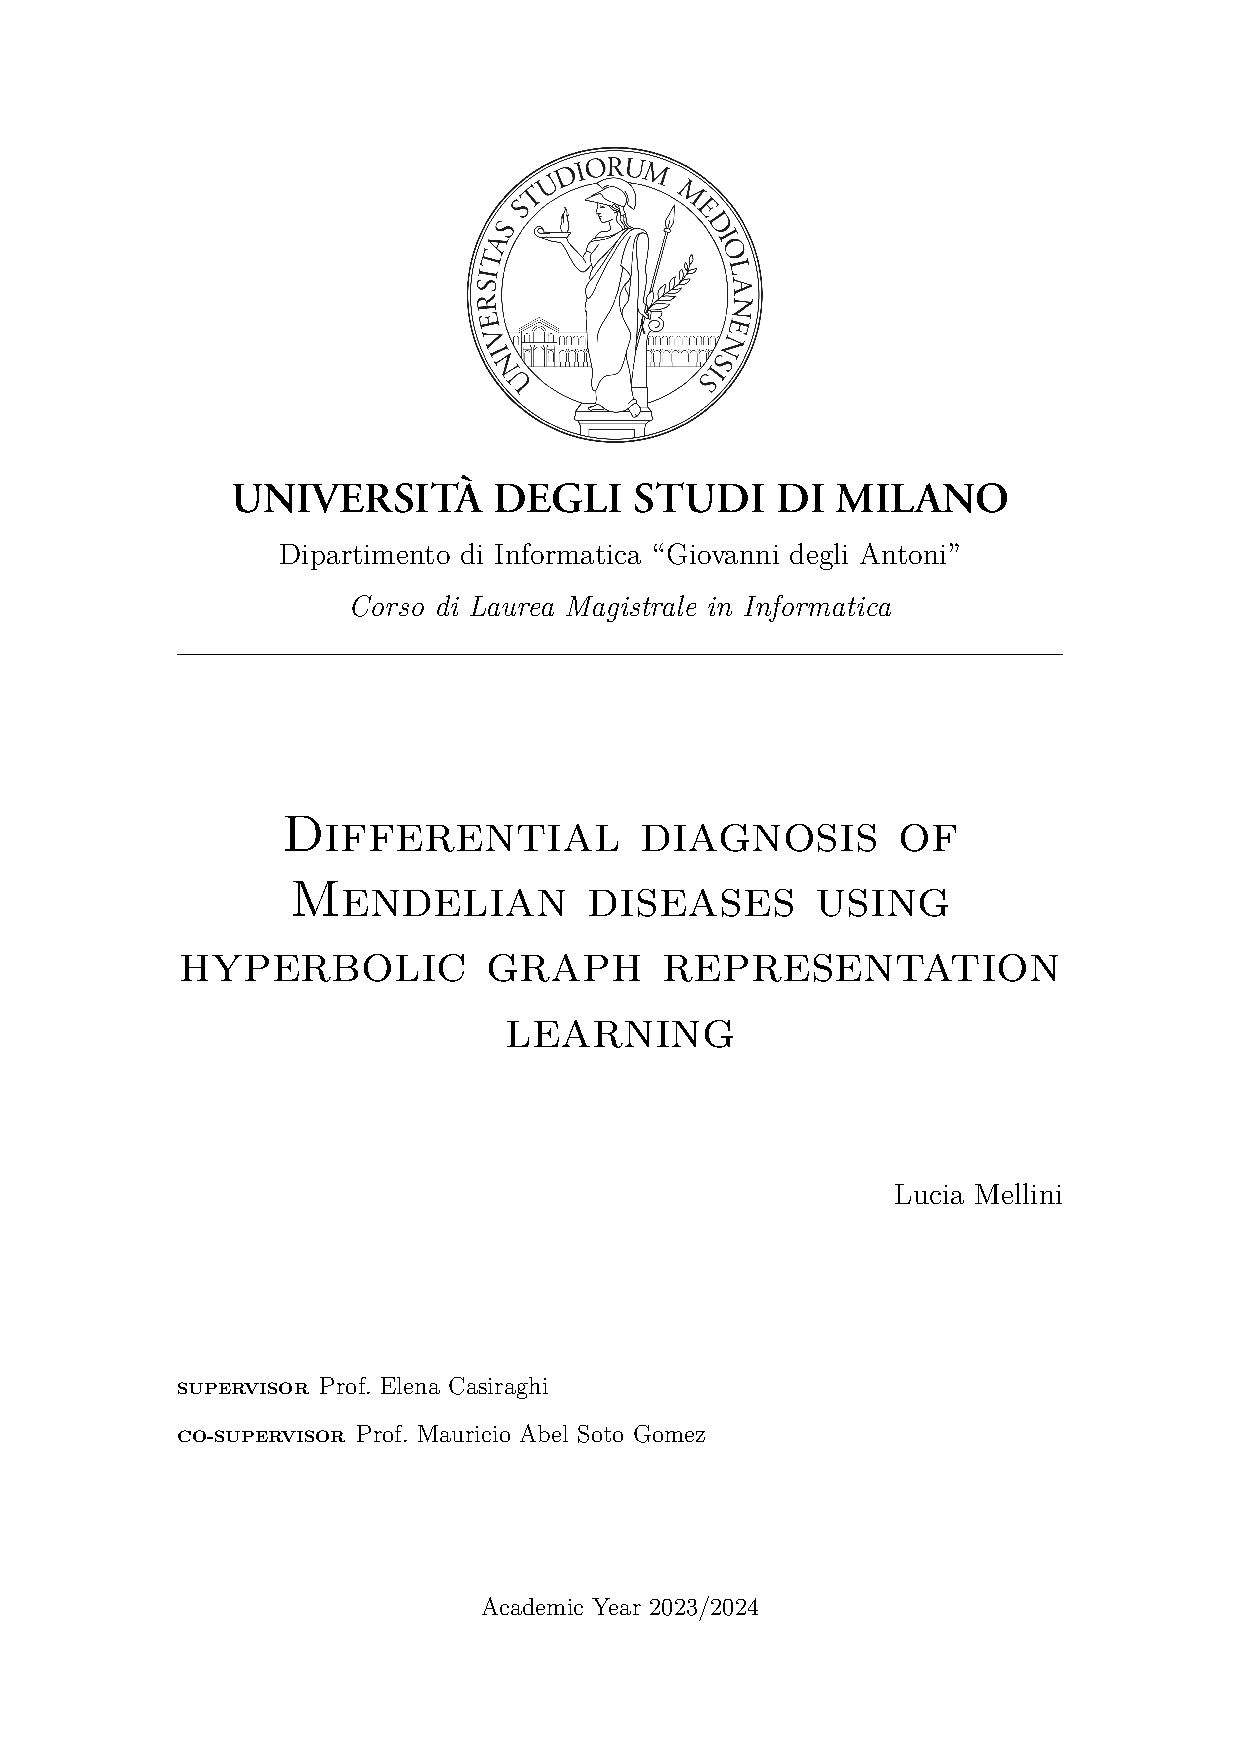
\includepdf{titlepage.pdf}
%\maketitlepage

\frontmatter


\maketitle

\tableofcontents
   
\mainmatter

\setcounter{chapter}{-1}
\chapter{Introduction}
% In the past year literature has seen significant efforts in the automated collection, integration, and analysis of the vast amount of heterogeneous biomedical information published online. This information can be semi-automatically mined from various knowledge bases, harmonized and standardized, and condensed into integrated biomedical information structures known as knowledge graphs (KGs). In these graphs, information is represented by entities or concepts (such as proteins, drugs, and chemical compounds), which are nodes linked by edges representing known relationships.

% Prominent examples of biomedical knowledge graphs in the past five years include those used for COVID-19 research~\cite{ReeseJustinT.2021KAFt}, the discovery of key exposure factors for female reproductive disorders~\cite{ChanLaurenE2024Pnae}, and investigations into RNA molecules to infer new RNA targets for personalized treatments\cite{CavalleriEmanuele2024Aokg}. To extract meaningful knowledge from these graphs, graph representation learning techniques have been proposed\cite{Hamilton2020GraphRL}, \cite{li2022graphrepresentationlearningbiomedicine}. These techniques compute representative embeddings for graph elements and use these embeddings to predict unknown categories of nodes or edges or the existence of edges between nodes.

% Despite the progress in data integration research, a clear divide remains between two predictive strategies, as pointed out in the vision of individualized knowledge graphs\cite{PingPeipei2017IKGA}. On one side are predictive methods that work on datasets representing specific cases, which often yield knowledge that is not generalizable enough to be applied to compute reliable predictions on novel cases. On the other side are methods that work on KGs to uncover broad, static knowledge that is often too general for practical application. What is missing is an approach that enables predictions on specific sample data using the broad knowledge from KGs, while also deriving new relationships within a KG based on information from specific sample data. To address this issue, the first challenge is to connect these two knowledge sources. This requires an investigation into how nodes representing specific patients or samples can be linked to nodes representing broader concepts, such as genes or specific RNA molecules. Secondly, given the vast number of nodes in a KG compared to the often limited number of cases in medical studies, new techniques should be developed to process a KG in a way that biases its representation to retain information from less represented nodes.

% In \Cref{kgs} and \Cref{grl} we present the theoretical background and applications of knowledge graphs and graph representation learning.

\newpage
\section*{Structure of the thesis}
The work is organized as follows:
\begin{description}
    \item[\Cref{kgs}] gives an overview of knowledge graphs: their structure, how to deduce and induce information from them. Seen our scope we then focus on knowledge graphs used in the biomedical domain.
    \item[\Cref{grl}] introduces graph representation learning, a technique to learn succinct descriptions of graphs. We go through the evolution of this approach to justify the methods currently used. In \Cref{sec:embeddingsKGs} we delve into how graph representation learning has been adapted for knowledge graphs.
    \item[\Cref{hyperbolic}] highlights some geometry concepts to understand the intuition behind hyperbolic geometry, its connection to tree metric spaces and the tools to build learning models that operate in hyperbolic spaces. 
    \item[\Cref{hrl}] explores hyperbolic representation learning methods for hierarchical graphs, with a focus on the HGCN technique.
\end{description}
\part*{Background}
\chapter{Knowledge Graphs}\label{kgs}
This chapter presents a comprehensive examination of knowledge graphs, elucidating their theoretical underpinnings and a range of applications. The discussion begins with a formal definition of knowledge graphs in Sections~\ref{definition}-~\ref{inductive-information}, followed by an exploration of their specific applications within the life sciences in Section~\ref{kgs:biomed}.

\section{Definition}\label{definition}
The concept of knowledge graphs has garnered significant attention since Google's introduction of its Knowledge Graph in 2012, particularly within the realm of Semantic Web research. However, despite their widespread utilization, a consensus on a singular definition remains elusive, as academic sources provide diverse interpretations. The following definitions exemplify this variation:

\begin{description}
    \item[Structural and compositional aspects] Knowledge graphs are characterized by graph-based representations of information. Paulheim~\cite{Paulheim2016KnowledgeGR} defines a knowledge graph as an entity-focused graph that (i) illustrates real-world entities alongside their interrelations, (ii) establishes classes and relations within a defined schema, (iii) facilitates the interrelation of arbitrary entities, and (iv) encompasses various topical domains. Echoing this, the Journal of Web Semantics~\cite{Kroetsch2016knowledge} characterizes knowledge graphs as comprised of entities, their types, and the relationships among those entities.
    
    \item[Domain-specific representations] According to the Semantic Web Company, knowledge graphs can adapt to represent structures specific to varied fields, encompassing concepts, documents, and datasets.    
    
        \item[Formal definition] Färber et al.~\cite{Farber2016linked} articulate knowledge graphs as RDF graphs (introduced in Section~\ref{models:directed_edge_labeled_graphs}), which consist of a collection of $(s, p, o)$ triples, where:
    \begin{itemize}
        \item $s\in U \cup B$ denotes a subject,
        \item $o\in U\cup B\cup L$ denotes an object,
        \item $p\in U$ denotes a predicate
    \end{itemize}
    Here, an RDF term can be represented as a URI ($u\in \mathcal{U}$), a blank node ($b\in \mathcal{B}$), or a literal ($l\in \mathcal{L}$).
    
    \item[Dynamic extraction] An emphasis on the automatic extraction of interconnected facts from the web has been presented by Pujara et al.~\cite{Pujara2013KGIdentification}.
\end{description}

The aforementioned diversity in definitions complicates discussions and comparative studies, emphasizing the need for a common definition. In response to this requirement, Ehrlinger et al.~\cite{Ehrlinger2016TowardsAD} propose the following definition for knowledge graphs:
\begin{center}
    \begin{quote}
        A knowledge graph acquires and integrates information into an ontology and applies a reasoner to derive new knowledge.
    \end{quote}
\end{center}
This definition contributes to a unified comprehension of knowledge graphs through three salient aspects:
\begin{description}
    \item[Data integration] Knowledge graphs gather and incorporate data from disparate sources, which renders them both dynamic and expandable.
    \item[Inference capabilities] The employment of reasoning engines facilitates the deduction of new information, thereby augmenting the functionality beyond that of static data repositories.
    \item[Ontological basis] The foundation of knowledge graphs rests on ontological structures, which provide a formal framework for the representation of knowledge and relationships.
\end{description}

Knowledge graphs exhibit a complexity that surpasses that of traditional databases or ontologies, combining the beneficial properties of both to enable automated reasoning and the dynamic incorporation of information. In this context, the functionality and capabilities of knowledge graphs are deemed to be of greater significance than their possible great size.

\section{Data Graphs}\label{data-graphs}
The foundational concept of knowledge graphs is based on the transformation of data into a graph structure, resulting in what is referred to as a \term{data graph}. This methodology confers enhanced flexibility in integrating new data sources, in contrast with relational models, which necessitate predefined schemas. Although tree structures offer analogous adaptability, graph structures do not impose hierarchical constraints and permit the existence of cycles. We explore  various graph-structured data models that can be employed to represent such graphs, as listed in~\cite{Hogan2021KGs}. We then describe various enhancements and extensions of the data graph – relating to schema, identity and context – that provide additional structures for accumulating knowledge.

Further formal details pertinent to the subsequent sections can be found in Appendix~\ref{app:data-graphs}.

\subsection{Models}\label{models}
The principal graph structures utilized to represent knowledge graphs are delineated in this section, progressively introducing increasingly complex models.

\subsubsection{Directed Edge-Labeled Graphs}\label{models:directed_edge_labeled_graphs}
A directed edge-labeled graph is composed of a set of nodes and a set of directed, labeled edges interconnecting these nodes. Within knowledge graphs, nodes correspond to entities, while edges represent the relationships between them. The Resource Description Framework (RDF)~\cite{Cyganiak2014rdf}, as endorsed by the World Wide Web Consortium (W3C)\footnote{More details about RDFs at \url{https://www.w3.org/TR/rdf12-concepts/}}, represents a standard data model. This model specifies node types including Internationalized Resource Identifiers (IRIs)\footnote{Section of the W3C working draft on RDFs regarding IRIs \url{https://www.w3.org/TR/rdf12-concepts/\#section-IRIs}} for global identification, literals for strings and datatype values, as well as blank nodes for anonymous nodes.

\subsubsection{Heterogeneous Graphs}
Heterogeneous graphs provide a generalization of directed edge-labeled graphs by permitting nodes and edges to possess varying \term{types}. Edges can be classified as \term{homogeneous} when connecting nodes within the same property or \term{heterogeneous} when linking nodes of different types. This classification enables the partitioning of the graph by node types, which is advantageous for machine learning applications.

\subsubsection{Property Graphs}
Property graphs augment the flexibility of graph structures by incorporating \term{property-value} pairs and assigning a \term{label} to both nodes and edges. Attribute graphs can be transformed to and from directed edge-labeled graphs without loss of information. Although both models are equivalent in terms of representational capacity, directed edge-labeled structures are characterized by a more minimalistic framework, whereas property graphs offer greater flexibility. The choice between these models is contingent upon practical considerations, such as the availability of implementations.

\subsubsection{Additional Graph Data Models}
Extensions of traditional graph models include \term{complex nodes} or \term{hypernodes} that encapsulate edges or nested graphs. In contrast, \term{hypergraphs} define \term{complex edges} that connect more than two nodes simultaneously.

\subsection{Querying}\label{querying}
Several languages exist for the analysis of graph structures. SPARQL is utilized for querying RDF graphs~\cite{Harris2013SPARQL}, while graph databases may employ query languages such as Cypher~\cite{Francis2018Cypher}, Gremlin~\cite{Rodriguez2015Gremlin}, and G-CORE~\cite{Angles2018G-CORE}~\cite{Angles2017FoundationmodernQueryLnguagesforGraphDatabases}. Common elements of these languages include graph patterns, relational operators, and path expressions.

\subsubsection{Graph Patterns}
At the core of graph query languages are \term{(basic) graph patterns}, which are intrinsically linked to the graph framework. In the context of directed edge-labeled graphs, the fundamental components consist of nodes and edge labels. In attribute graphs, these components include identifiers, tags, attributes, and values.

Terms are categorized into constants and variables. The evaluation of graph patterns involves generating mappings from variables to constants, ensuring that the graph pattern's image is contained within the graph.

The variables in the graph patterns could be mapped to the same constant terms; however, such instances may not always be desirable. The underlying semantics may include:
\begin{itemize}
    \item \term{Homomorphism-based semantics}, which permits multiple variables to map to identical components.
    \item \term{Isomorphic-based semantics}, which stipulates distinct mappings for nodes and edge variables.
\end{itemize}

\subsubsection{Complex Graph Patterns}
Graph patterns can convert an input graph into a result table, which may then be manipulated using relational algebra. The operations applicable include:
\begin{itemize}
    \item Unary operations:
    \begin{itemize}
        \item \term{Projection ($\pi$)} to extract a subset of columns,
        \item \term{Selection ($\sigma$)} to extract a subset of rows,
        \item \term{Column renaming ($\rho$)}.
    \end{itemize}
    \item Binary operations:
    \begin{itemize}
        \item \term{Union ($\cup$)} to merge rows from two tables,
        \item \term{Difference (-)} to exclude rows from one table that are present in another,
        \item \term{Joins ($\bowtie$)} to merge rows from two tables based on a related column.
    \end{itemize}
\end{itemize}
Graph patterns can thus be articulated within a subset of relational algebra comprising $\pi$, $\sigma$, $\rho$, and $\bowtie$.

\subsubsection{Navigational Graph Patterns}
A distinguishing feature of graph query languages is the incorporation of \term{path expressions} within queries. A path expression $r$ serves as a regular expression that encompasses paths of arbitrary lengths, which can be articulated as a \term{regular path query} $(x,r,y)$. The recursive nature of regular path queries is established as follows: a base path expression $r$ is a constant edge label. If $r$ is a path expression, its inverse $r^-$ along with the Kleene star $r^*$ also qualify as path expressions. Furthermore, if $r_1$ and $r_2$ denote path expressions, their disjunction $r_1 \mid r_2$ and concatenation $r_1 \cdot r_2$ remain path expressions.

Evaluation semantics for regular path queries must account for loops, which may yield infinite matching expressions. Options for management include the return of the shortest paths or those devoid of repeated nodes and edges. Alternatively, it is possible to return merely pairs of nodes linked by a matching path without detailing the entire path.

\subsection{Schema}\label{schema-identity-context}
Henceforth, we refer to a \term{data graph} as a collection of data represented as nodes and edges using one of the models discussed in~\ref{data-graphs}. We refer to a \term{knowledge graph} as a data graph potentially enhanced with representations of schema, identity, ontologies and/or rules. These additional representations may be embedded in the data graph, or layered above it.

Modeling data as graphs enables the deferral or circumvention of explicit schema definitions. Schemata can delineate high-level structures or semantic elements, leading to the categorization of \term{semantic}, \term{validating}, and \term{emergent} schemata.

\subsubsection{Semantic Schema}\label{schema_semantic}
A \term{semantic schema} delineates the meanings of high-level terms (\term{vocabulary}) utilized within the graph, thereby facilitating inferential reasoning. Natural groupings of nodes may be classified as \term{classes}, with hierarchical relationships established where child classes are designated as \term{subclasses} of their respective parents.

Edge labels, also referred to as \term{properties}, may be systematically organized into hierarchies, with specific attributes serving as \term{sub-properties} of broader properties. The \term{domain} of properties indicate the properties of objects to which nodes are connected. Conversely, \term{range} specifies the properties of objects to which nodes are connected through the property.

The \textit{RDF Schema} (RDFS) standard~\cite{Brickley2014RDFSchema1.1} establishes definitions for subclasses, subattributes, domains, and ranges applicable to RDF graphs. Semantic illustrations inherent to these features are presented in Table~\ref{tab:semanticSchemaFeatures}. The \textit{Web Ontology Language} (OWL) standard~\cite{Hitzler2014OWLPrimer} offers expanded definitions.

Typically, semantic schemas are constructed for graph data that may be incomplete. The absence of a specific edge does not necessarily imply the nonexistence of the relationship in actuality. Such systems operate under the \term{Open World Assumption} (\term{OWA}), as opposed to the \term{Closed World Assumption} (\term{CWA}). The CWA allows for definitive assertions regarding the existence of relationships. Consequently, the introduction of an edge may challenge previous assumptions, while the OWA maintains that a conclusively proved false statement remains false, despite the addition of further edges.

\newcommand{\conditiondiagram}[6]{%
    \begin{tikzpicture}[scale=0.8,baseline=(x.base), ->, thick]
        % First node and edge
        \node[draw, circle] (x) at (0, 0) {\(#1\)};
        \node[draw, circle] (y) at (2, 0) {\(#2\)};
        \draw (x) -- node[above] {\(#3\)} (y);

        % Optional implication arrow and second relationship
        \ifx#4\empty\else
            \node at (3, 0) {\(\implies\)};
            \node[draw, circle] (x2) at (4, 0) {\(#4\)};
            \node[draw, circle] (y2) at (6, 0) {\(#5\)};
            \draw (x2) -- node[above] {\(#6\)} (y2);
        \fi
    \end{tikzpicture}
}

\begin{table}
    \setlength{\textwidth}{0.8\textwidth}
    \centering
    \renewcommand{\arraystretch}{2}
    \begin{tabular}{lcc}

    \toprule
    \textbf{Feature} & \textbf{Definition} & \textbf{Condition} \\
    \midrule

    \textit{Subclass} 
        & \conditiondiagram{c}{d}{\text{\footnotesize subc.\ of}}{}{}{}
        & \conditiondiagram{x}{c}{\text{\footnotesize type}}{x}{d}{\text{\footnotesize type}} \\
        
    \textit{Subproperty} 
        & \conditiondiagram{p}{q}{\text{\footnotesize subp.\ of}}{}{}{}
        & \conditiondiagram{x}{y}{\footnotesize p}{x}{y}{\footnotesize q} \\
    
    \textit{Domain} 
        & \conditiondiagram{p}{c}{\text{\footnotesize domain}}{}{}{}
        & \conditiondiagram{x}{y}{\footnotesize p}{x}{c}{\text{\footnotesize type}} \\

    \textit{Range} 
        & \conditiondiagram{p}{c}{\text{\footnotesize range}}{}{}{}
        & \conditiondiagram{x}{y}{\footnotesize p}{y}{c}{\text{\footnotesize type}} \\
        \bottomrule
    \end{tabular}
    \caption{Definitions for subclass, subproperty, domain, and range features in semantic schemata}
    \label{tab:semanticSchemaFeatures}
\end{table}
    

\subsubsection{Validating Schema}
In scenarios where graphs represent a broad spectrum of diverse and incomplete data, the OWA is deemed more appropriate. Nevertheless, circumstances may arise where it is imperative to establish that the data graph is "complete." Thus, a \term{validating schema} can be defined to enforce constraints upon the data graph and identify any violations. While semantic schemata primarily infer new data, validating schemata assess the integrity of existing data.

A prevalent methodology for the definition of a validating schema involves the utilization of \term{shapes}~\cite{Knublauch2017SHACL, LabraGayo2017ValidatingRDF, Prudhommeaux2014ShapeExpressions}. A shape \term{targets} specific nodes and specifies necessary \term{constraints}. The identification of the target may manifest in various forms, such as instances of a specific property, the domain or range of an attribute, or outcomes derived from a query. Constraints may impose restrictions on the quantity or types of values that attributes can assume. An \term{open shape} permits the inclusion of additional attributes, whereas a \term{closed shape} imposes stricter limitations.

Validating and semantic schemata can function synergistically, with validation applicable to data graphs inclusive of inferred data. Open shapes may be favored when enumerating constraints across all potential attributes.

\subsubsection{Emergent Schema}
While semantic and validating schemata necessitate explicit definitions and constraints, it is acknowledged that a data graph may inherently exhibit latent structures, which can be extracted through an \term{emergent schema}~\cite{Pham2015EmergenSchemaFromRDF} or a \term{graph summary}~\cite{Cebiric2019SummarizingSemanticGraphs, Liu2018GraphuSummarizationMethodsAndApplications, Spahiu2016ABSTAT}. A prevalent design in this regard is represented by quotient graphs, which partition nodes based on an equivalence relation while preserving structural properties of the graph. Merging the nodes within each partition into a singular node generates a quotient graph.

Each node in the quotient graph corresponds to a partition of the original nodes, with an edge $(X,Y)$ is in the quotient graph if there exist $x\in X$ and $y\in Y$ such that $(x,y)$ constitutes an edge within the data graph.

Although a quotient graphs can be defined in various ways, it is imperative that they \term{simulate} its input graph. For all input nodes $x$ and quotient nodes $X$ such that $x\in X$, if $(x,y)$ is an edge in the data graph, then a corresponding edge $(X,Y)$ must exist in the quotient graph with $y\in Y$. A more stringent condition, \term{bisimilarity}, stipulates that if $(X,Y)$ is an edge in the quotient graph, then for every $x\in X$, there exists a $y\in Y$ such that $(x,y)$ exists within the data graph. Formal definitions for these concepts are provided in Appendix~\ref{app:emergent-schema}.
For each possible partition of the data graph nodes there exists a  corresponding quotient graph. Other forms of similar or bisimilar graphs may be articulated according to the (bi)simulation relations~\cite{Cebiric2019SummarizingSemanticGraphs}. Such methodologies condense the data graph into a more abstract topology. Nodes may be assigned labels that represent the cardinality of partitions or high-level labels, foregoing the necessity of retaining all node labels.

\subsection{Identity}\label{identity}
To mitigate ambiguity one can adopt globally unique identifiers, as well as the incorporation of external identity edges to disambiguate nodes.

Merging multiple knowledge graphs may introduce ambiguities, resulting in naming conflicts. \term{Persistent Identifiers} (PIDs) serve to uniquely identify entities (for instance, DOI for academic papers, ORCID for authors, ISBN for books). The RDF specification advocates for the use of Internationalized Resource Identifiers (IRIs) to differentiate between web pages and tangible objects~\cite{Hakala2010PIDs}.

While HTTP IRIs facilitate global identification, they do not inherently assure persistence. \term{Persistent URL} (PURL) services provide stable identifiers that redirect to current locations, thereby ensuring that references remain valid~\cite{BernersLee2006LinkedData}\cite{Heath2011LinkedData}.

Even with the utilization of IRIs, disparate knowledge graphs may employ different identifiers to refer to the same entity. To manage these cases the OWL standard for example encompasses the construct \texttt{owl:sameAs} to establish equivalence.
Identifiers may not convey semantic significance. For instance, Wikidata utilizes numerical IRIs to maintain language neutrality. RDF graphs typically include additional metadata such as labels, aliases, and comments. Multilingual lexicalized knowledge graphs further facilitate object recognition across different languages~\cite{DeMelo2015Lexvo.org, MartinezRodriguez2020InformationExtractionMeetsSemanticWeb}.  

In certain instances, graphs must represent unidentified objects using existential nodes (or blank nodes within RDF). Techniques such as skolemization may be employed to assign canonical labels, though some scholars advocate minimizing their application~\cite{Cyganiak2014rdf, Hogan2017CanonicalFormsIsomorphicEquivalentRDFGraphs, Longley2019RDFDatasetNormalization}.

\section{Deductive Information}\label{deductive-information}
The capacity for humans to infer additional information from a data graph transcends the explicit relationships denoted by edges. By utilizing data as foundational premises alongside some a priori general rules about the world, new data can be deduced. Such rules are classified as ``commonsense information''~\cite{McCarthy1990FomalizingCommonsense} or ``domain information''.

For machines to perform analogous deductions, formal instructions are required. Entailment regimes are employed to normalize conclusions that logically follow from initial premises. The ability to make these deductions enhances query response accuracy, classification, and inconsistency detection.

Although we have already discussed in Section~\ref{schema_semantic} how semantic schemata can capture subclass relations, we now discuss how more complex entailments can be captured and automated. Though one could leverage logical frameworks like First-Order Logic, we focus on ontologies which constitute a formal representation of knowledge that, importantly for us, can be represented as a graph.

\subsection{Ontologies}\label{ontologies}
For successful entailment, precision concerning the meanings of terms is imperative. Since there is no ``correct'' meaning for a given term we may, its definition is a matter of convention.

The term ``ontology'' originates from philosophical discourse regarding the nature of existence. In the computing context, an \term{ontology} indicates a concrete, formal representation of the meanings attributed to terms within a specified domain.

The practical utility of an ontology is contingent upon consensus, detail, and adoption. Widespread adoption fosters consistent terminology and modeling practices, while agreement promotes interoperability.

Widely recognized ontology languages encompass the \textit{Web Ontology Language} (\textit{OWL})~\cite{Hitzler2014OWLPrimer} and the \textit{Open Biomedical Ontologies Format} (\textit{OBOF})~\cite{Mungall2012OBOF}.

\subsubsection{Interpretation}
It is possible to interpret a node or edge as corresponding to a tangible object or relation. The data graph can be conceptualized as a \term{domain graph}. The interpretation process entails mapping nodes and edges from the data graph to entities and relations within the domain graph. An \term{interpretation} is characterized by a domain graph and a mapping function that aligns the data graph to the domain graph. The domain graph adheres to the same modeling principles as the data graph. Under the Open World Assumption (OWA) (recall from Section~\ref{schema_semantic}), if an edge does not exist between two nodes in the data graph, similarly it cannot exist in the domain graph, since what is not known is assumed to be false. Conversely, under the Open World Assumption (OWA), we cannot be certain that this relation does not exist as this could be part of some knowledge not (yet) described by the graph. 

These foundational assumptions delineate the validity of interpretations, and which interpretations \term{satisfy} a given data graph. Additional assumptions pertain to the uniqueness of terms. The \term{Unique Name Assumption} (\term{UNA}) forbids interpretations that map two distinct data terms to a singular domain term, while the \term{No Unique Name Assumption} (\term{NUNA}) permits such interpretations.
\term{Semantic conditions} define the criteria for valid interpretations of a graph. As an illustration, if $p$ is a subclass of $q$, one could enforce that if the tuple $(x,y,p)$ is present in the domain graph, then the edge $(x,y,q)$ must exist.

\subsubsection{Model-Theoretic Semantics}
Interpretations that fulfill a graph's requirements are designated as \term{models}. Under the OWA, a model may accommodate more edges than those delineated in the data graph. To refine the constraints on models, the inclusion of \term{axioms} can enforce conditions that interpretations must achieve. Such axioms are presented similarly to the definitions outlined in Table~\ref{tab:semanticSchemaFeatures}.

\subsubsection{Entailment}
A graph \term{entails} another graph if every model consistent with the former is also a model of the latter. The latter graph conveys no additional information beyond what is contained within the former.

The determination of whether one graph entails another remains undecidable\footnote{A decision problem is said to be undecidable when there does not exist an algorithm that halts on all inputs with the correct answer.}~\cite{Hitzler2010FoundationsSWTechnologies}. However, practical reasoning algorithms can be developed that:
\begin{enumerate*}[label=(\roman*),before=\unskip{ i.e., }, itemjoin={{, }}, itemjoin*={{, or }}]
    \item\label{opt_1} halt on any input but may overlook certain entailments,
    \item\label{opt_2} consistently halt with accurate results but only accommodate restricted input ontologies,
    \item\label{opt_3} exclusively yield correct results but may never halt on certain inputs.
\end{enumerate*}

Option \ref{opt_3} has been explored by using theorem provers~\cite{Schneider2011ReasoningOWL2Full}. Options \ref{opt_1} and \ref{opt_2} are more frequently pursued, employing rules or Description Logics. Option \ref{opt_1} is conducive to efficient reasoning, particularly in contexts where data may be incomplete. In contrast, option \ref{opt_2} may be more suitable in domains where the omission of entailments is deemed undesirable.

\section{Inductive Information}\label{inductive-information}
While deductive knowledge is characterised by precise logical consequences, inductive information concerns the process of generalizing patterns derived from observations to generate novel predictions. Then \term{inductive knowledge} includes both the models used to encode patterns, as well as the predictions made by those models.
A variety of inductive methodologies are applicable to knowledge graphs. Unsupervised techniques leverage graph analytics to identify communities or clusters, as well as to discern central nodes and edges. Knowledge graph embeddings utilize self-supervision to derive low-dimensional numerical representations. The graph structure itself can also be advantageous for supervised learning approaches. Symbolic learning techniques possess the ability to derive symbolic models – i.e., logical formulae in the form of rules or axioms – from graphs in a self-supervised fashion. A discussion of supervised learning techniques applicable to knowledge graphs is presented in the subsequent chapter.

\section{Biomedical Knowledge Graphs}\label{kgs:biomed}
In biomedical research, traditional databases fail to capture the intricate relationships within molecular interactions, pharmacological properties, and clinical records~\cite{Callahan2020KBDS}\cite{Su2020NetworkEmbeddingBiomedicalbDS}. \term{Biological knowledge graphs} (\term{BKG}) overcome these limitations by structuring heterogeneous data like molecular interactions, pharmacological datasets, and clinical records, and facilitating tasks like disease modeling and personalized medicine or drug discovery~\cite{Lu2025BiomedicalKG}. We shortly review BKGs, categorizing them into domains, discussing key tasks, and  highlighting real-world applications.

Despite their transformative potential, BKGs face challenges related to data integration, scalability, and interpretability. The heterogeneous nature of biomedical data, inconsistencies in terminology, and the exponential growth of biomedical knowledge make it difficult to maintain accurate and up-to-date BKGs. Scalability remains a concern, particularly in processing large-scale networks and executing complex queries efficiently. Moreover, interpretability issues persist, as users often struggle to navigate intricate network structures and understand the reasoning behind AI-driven predictions.

\subsection{Domains}
Biomedical knowledge graphs (BKGs) serve as structured frameworks that integrate and analyze complex biomedical data across multiple domains. These domains encapsulate diverse sources of knowledge, each contributing to the construction and application of BKGs in distinct yet interconnected ways. We list three primary domains, and for each we reference some BKG examples:
\begin{description}
    \item[Multi-omics] focusing on genomic~\cite{Jha2019genomicsKG}, transcriptomic~\cite{CavalleriEmanuele2024Aokg}, and proteomic~\cite{Zhang2022ontoprotein} data, supporting research in disease mechanisms and biological pathways.
    \item[Pharmacology] are instrumental in modeling interactions like drug-disease and drug-target~\cite{Gonzalez2023drugmechdb}, predicting adverse drug reactions, and facilitating drug repurposing efforts~\cite{Huang2024foundationModelDrugRepurposing}.
    \item[Medical knowledge] integrating electronic health records~\cite{Shang2021ehr} and clinical knowledge to improve diagnosis, treatment recommendations, and healthcare decision-making. Some disease specific BKGs stand out for conditions like hepatocellular carcinoma~\cite{Li2020kghc} or COVID-19~\cite{Zheng2021multiModalKGCOVID19}.
\end{description}
Some BKGs span multiple domains, creating comprehensive frameworks that enable cross-disciplinary insights.

\subsection{Tasks \& applications}
Beyond their structural aspects, BKGs enable four key tasks: 
\begin{description}
    \item[Knowledge management] involves structuring raw biomedical data~\cite{Percha2018globalNetworkBiomedicalRelationshipsDerivedText}\cite{Sang2018sematyp}, transforming disparate datasets into standardized formats, and integrating multiple sources into a unified framework~\cite{Himmelstein2017Hetionet}.
    \item[Knowledge retrieval] leverages BKGs to enhance data visualization, statistical analysis, and knowledge enhancement though query-based information retrieval~\cite{Pan2024unifyingLLMsKGs}\cite{Soman2024biomedicalKGOptimizedPromptGenerationForLLMs}, allowing researchers and clinicians to quickly access relevant biomedical insights.
    \item[Knowledge reasoning] encompasses inference and prediction, enabling the discovery of novel relationships, such as identifying potential drug candidates~\cite{Huang2024foundationModelDrugRepurposing} or predicting disease-drug links~\cite{li2022graphrepresentationlearningbiomedicine}.
    \item[Knowledge interpretation] ensures the reliability of these predictions by tracing the reasoning process through logical explanations (e.g ~\cite{Jimenez2024explainableDrugRepurposing} visualises reasoning paths for drug repurposing) or assisted interpretation using AI-driven systems~\cite{ONeil2024phenomicsAssistant}.
\end{description}

The applications of BKGs extend across multiple biomedical fields. In clinical decision support, BKGs assist in diagnosing diseases, predicting health risks~\cite{Tao2020miningHealthKnowledgeHealthRiskPrediction}, and recommending personalized treatments. In drug discovery, they play a crucial role in identifying potential drug candidates, repurposing existing medications (like for COVID-19 ~\cite{Zhang2021drugRepurposingForCovid19}), and predicting adverse drug reactions~\cite{Abdelaziz2017largeScaleMiningKGDrugDrugInteractions}. Additionally, BKGs support scientific research by facilitating hypothesis generation and uncovering new research opportunities. They also enhance intelligent question-answering systems, helping to improve the accuracy and reliability of AI-driven medical chatbots~\cite{Shu2024KG-LLM}\cite{Sung2021canLMBeKnowledgeBases} and literature retrieval tools.


\chapter{Graph representation learning}\label{grl}

\section{Graph learning problems}
Machine learning is inherently a problem-driven discipline. We seek to build models that can learn from data in order to solve particular tasks, and machine learning models are often categorized according to the type of task they seek to solve: supervised or unsupervised. Learning with graphs is no different, but the usual categories of supervised and unsupervised are not necessarily the most informative or useful when it comes to graphs. In this section we provide a brief overview of the most important and well-studied machine learning tasks on graph data. As we will see machine learning problems on graphs often blur the boundaries between the traditional machine learning categories.

\subsection{Node classification}
Given a graph $G=(V,E,L)$ in \term{node classification} the goal is to predict the label associated with each node $v\in V$, when we only given the true labels on a \term{training set} of nodes $V_\text{train}\subset V$. Often one assumes that we only have label information for a small subset of nodes, but there are instances that involve many labeled nodes, like classifying the function of proteins in the interactomes of different species~\cite{Hamilton2017inductive}.
Even though node classification appears to be a straightforward variation of standard supervised learning, there are important differences. The nodes in a graph, in fact, are not independent and identically distributed since we are modelling an interconnected set of nodes. The key insight behind many of the most successful node classification approaches is to explicitly leverage the connections between nodes. One particularly popular idea is to exploit \term{homophily}, which is the tendency for nodes to share attributes with their neighbors in the graph~\cite{Mcpherson2001homophilyInSocialNw}. For example, people tend to form friendships with others who share the same interests or demographics. Based on the notion of homophily we can build machine learning models that try to assign similar labels to neighboring nodes in a graph~\cite{Zhou2003LearningLocalGlobalConsistency}. Beyond homophily there are also concepts such as structural equivalence~\cite{Donnat2017GraphWaveletsStructuralRoleSimilarityComplexNws}, which is the idea that nodes with similar local neighborhood structures will have similar labels, as well as \term{heterophily}, which presumes that nodes will be preferentially connected to nodes with different labels. When we build node classification models we want to exploit these concepts and model the relationships between nodes, rather than simply treating nodes as independent datapoints.

\subsection{Link prediction}
The standard setup for \term{link prediction} is that we are given a set of nodes $V$ and an incomplete set of edges between these nodes $E_\text{train} \subset E$. Our goal is to use this partial information to infer the missing edges $E \setminus E_\text{train}$. This is one of the most popular machine learning tasks with graph data, and has countless applications, like predicting drug side-effects~\cite{Zitnik2018ModelingPolypharmacySideEffectsGCN}. In complex multi-relational graph datasets, such as BKGs that encode hundreds of different biological interactions, link prediction can require complex reasoning and inference strategies~\cite{Nickel2015ReviewRelationalMLKG}. Ofter link prediction requires inductive biases that are specific to the graph domain.

\subsection{Clustering and community detection}
Both node classification and link prediction require inferring missing information about graph data, and in many ways, those two tasks are the graph analogues of supervised learning. Community detection, on the other hand, is the graph analogue of unsupervised clustering. The general intuition underlying the task of clustering is that the graph exhibits a community structure, where nodes are much more likely to form edges with nodes that belong to the same community. The challenge of community detection is to infer latent community structures given only the input graph $G = (V, E)$. The many real-world applications of community detection include uncovering functional modules in genetic interaction networks~\cite{Agrawal2018LargeScaleAnalysisDiseasePathwaysHumanInteractome}.

\subsection{Why graph representation learning?}
To solve the problems above there exist various ``traditional'' methods~\cite{Hamilton2020GraphRL}, such as the following:
\begin{itemize}
    \item graph statistics and kernel methods to extract feature information for classification tasks,
    \item neighbourhood overlap detection to provide heuristics for link prediction,
    \item spectral clustering and graph Laplacians to cluster nodes into communities.
\end{itemize}

However, these approaches are limited due to the fact that they require careful, hand-engineered statistics and measures. These hand-engineered features cannot adapt through a learning process, and designing these features can be a time-consuming and expensive process. The following chapters in this book introduce alternative approach to learning over graphs: graph representation learning. Instead of extracting hand-engineered features, we will seek to learn representations that encode structural information about the graph.

\section{Node embeddings}\label{sec:shallowEmbeddings}
The goal of these methods is to encode nodes as low-dimensional vectors or \term{embeddings} that summarize their graph position and the structure of their local graph neighborhood. In other words, we want to project nodes into a latent space, where geometric relations in this latent space correspond to relationships in the original graph~\cite{Hoff2002latentSpaceApproachesSocialNetworkAnalysis}. In \Cref{fig:nodeEmbedding} we illustrate this problem; our goal is to learn an encoder that maps nodes to a low-dimensional embedding space. These embeddings are optimized so that distances in the embedding space reflect the relative positions of the nodes in the original graph. 
\begin{figure}
    \centering
    \begin{tikzpicture}[scale=1.2, every node/.style={font=\small}]
        % Define styles
        \tikzstyle{node}=[circle, draw, fill=white, minimum size=5pt, inner sep=1pt]
        \tikzstyle{main_node}=[circle, draw, fill=red!50, minimum size=7pt, inner sep=1pt]
        \tikzstyle{arrow}=[->, thick, dashed]

        \node[node] (A) at (0.7,1) {};
        \node[node] (B) at (0,0.5) {};
        \node[node] (C) at (0.2,-0.9) {};
        \node[node] (D) at (2,0.5) {};
        \node[main_node, label=above:$u$] (U) at (1.2,0) {};
        \node[main_node, label=below:$v$] (V) at (2,-0.5) {};
        
        % Edges in the network
        \draw (A) -- (B) -- (C) -- (A);
        \draw (A) -- (U);
        \draw (U) -- (D);
        \draw (U) -- (V);
        \draw (D) -- (V);

        % Embedding space
        \node[ellipse, fill=black!20, minimum width=3cm, minimum height=3cm] (embedding) at (6,0) {};
        \node[below=0.2cm of embedding] {\textbf{embedding space}};

        % Embedded points
        \node[node, fill=white, label=right:$z_u$] (zu) at (6.5,0.8) {};
        \node[node, fill=white, label=right:$z_v$] (zv) at (6.3,-0.6) {};

        % Encoding arrows
        \draw[arrow] (U) to[out=20, in=160] node[above] {} (zu);
        \draw[arrow] (V) to[out=-20, in=200] node[below] {} (zv);

        % Labels
        \node[below=1.6cm of U] {\textbf{original graph}};
        \node[right=1.7cm of U] {encode nodes};
    \end{tikzpicture}
    \caption{Graph node encoding into embedding space}
    \label{fig:nodeEmbedding}
\end{figure}


We introducing the encoder-decoder framework as a way of explaining the workings of node embeddings. We then illustrate some node embedding methods; we especially focus on random walk approaches seen the techniques used s baseline during our experiments.

\subsection{An Encoder-Decoder framework}
We organize our discussion of node embeddings based upon the framework of encoding and decoding graphs, closely following the perspective in~\cite{Hamilton2020GraphRL}. In the encoder-decoder framework, we view the graph representation learning problem as involving two key operations. 
\begin{description}
    \item[Encoder] maps each node in the graph into a low-dimensional vector or embedding,
    \item[Decoder] takes the low-dimensional node embeddings and uses them to reconstruct information about each node's neighborhood in the original graph.
\end{description}
This idea is summarized in \Cref{fig:encDecFramework}.
In this section we focus on \term{shallow} embedding methods. The encoder can be generalized beyond the shallow embedding approach, for instance using node features or local graph structure around each node as input to generate the embedding, These generalized encoder architectures, often called graph neural networks (GNNs), are the focus of the next section.

\begin{figure}
    \centering
    \begin{tikzpicture}[scale=1.2, every node/.style={font=\small}]
        % Define styles
            \tikzstyle{node}=[circle, draw, fill=white, minimum size=4pt, inner sep=0.5pt]
            \tikzstyle{main_node}=[circle, draw, fill=red!50, minimum size=6pt, inner sep=0.5pt]
            \tikzstyle{arrow}=[->, thick, dashed]

            % First graph with rectangle
            \begin{scope}[xshift=-3.5cm]
            
                \node[node] (A) at (0.7,1) {};
                \node[node] (B) at (0,0.5) {};
                \node[node] (C) at (0.2,-0.9) {};
                \node[node] (D) at (2,0.5) {};
                \node[main_node, label=above:$u$] (U) at (1.2,0) {};
                \node[node] (E) at (2,-0.5) {};
            
            % Edges in the network
                \draw (A) -- (B) -- (C) -- (A);
                \draw (A) -- (U);
                \draw (U) -- (D);
                \draw (U) -- (E);
                \draw (D) -- (E);
            \end{scope}

            % Embedding representation
            \node[rectangle, fill=black!10, minimum width=0.2cm, minimum height=2.85cm] (embedding) at (0.8,0) {};
                        \foreach \y in {-0.9,-0.6,-0.3,0,0.3,0.6,0.9} {
                            \draw[white] (0.65,\y) -- (0.95,\y);
                        }
            \node[below=0.1cm of embedding] {$z_u$};

            % Arrows
            \draw[arrow] (U) -- node[above, align=center] {encode\\ node} (embedding.west);
            \draw[arrow] (embedding.east) -- node[above, align=center] {decode\\ neighbourhood} (4,0);

            % Decoded neighborhood (smaller version) with rectangle
            \begin{scope}[xshift=4cm,scale=0.8]
                \node[draw, rounded corners, minimum width=2.3cm, minimum height=2cm] at (1.4,0.3) {};
                \node[node] (A2) at (0.7,1) {};
                \node[node] (D2) at (2,0.5) {};
                \node[node] (E2) at (2,-0.5) {};
                \node[main_node, label=above:$u$] (U2) at (1.2,0) {};
                
                \draw (A2) -- (U2);
                \draw (U2) -- (D2);
                \draw (U2) -- (E2);
            \end{scope}
    \end{tikzpicture}
    \caption{Overview of the encoder-decoder framework}
    \label{fig:encDecFramework}
\end{figure}

\subsubsection{Encoder}
Formally, an \term{encoder} is a function that maps nodes to vector embeddings, so in the simplest case the encoder has the following signature:
\begin{equation*}
    \text{ENC}: V \to \mathbb{R}^d.
\end{equation*}
When talking about \term{shallow} node embeddings, the encoder function is simply an embedding lookup base on the node id. So for a node $v\in V$ we have that
\begin{equation}\label{eq:encoderLookup}
    \text{ENC}(v) = \mathbf{z}[v]
\end{equation}
where $\mathbf{z}\in \mathbb{R}^{V\times d}$ is a matrix containing the embedding vectors for all the nodes and $\mathbb{Z}[v]$ denotes the row of the matrix corresponding to node $v$.\

\subsubsection{Decoder}\label{sec:decoder}
The role of the \term{decoder} is to reconstruct certain graph statistics from the node embeddings that are generated by the encoder. For example, given the node embedding $\mathbf{z}_v$ of a node $v$ the decoder might attempt to predict its neighbourhood $\mathcal{N}(v)$.
The most common definition is a \term{pairwise} decoder, with the following signature:
\begin{equation*}
    \text{DEC}: \mathbb{R}^d \times \mathbb{R}^d \to \mathbb{R}^+.
\end{equation*}
Pairwise decoders are used to estimate relationships or similarities between pairs of nodes. For instance, a pairwise decoder can be used to predict if two nodes are neighbours in a graph.

Applying the pairwise decoder to a pair of embeddings $(\mathbf{z}_u, \mathbf{z}_v)$ results in the \term{reconstruction} of the relationship between nodes $u$ and $v$. The goal is to optimize the encoder and decoder as to minimize the reconstruction loss so that
\begin{equation}\label{eq:reconstruction}
    \text{DEC}(\text{ENC}(u), \text{ENC}(v)) = \text{DEC}(\mathbf{z}_u, \mathbf{z}_v) \approx \textbf{S}(u,v)
\end{equation}
where $\textbf{S}$ is a graph similarity measure between nodes. In the case of predicting edges in a graph the similarity function of a pair of nodes could be equivalent to the respective entry in the graph's adjacency matrix.

\subsubsection{Optimizing the Encoder-Decoder model}
To achieve the reconstruction objective (\Cref{eq:reconstruction}), the standard practice is to minimize an empirical reconstruction loss $\mathcal{L}$ over a set of training node pairs $\mathcal{D}$:
\begin{equation}\label{eq:loss}
    \mathcal{L} = \sum_{(u,v)\in\mathcal{D}} \ell(\text{DEC}(\mathbf{z}_u, \mathbf{z}_v), \textbf{S}[u,v])
\end{equation}
where $\ell: \mathbb{R}\times\mathbb{R}\to\mathbb{R}$ is a loss function measuring the discrepancy between the decoded similarity values $\text{DEC}(\mathbf{z}_u, \mathbf{z}_v)$ and the true values $\textbf{S}[u,v]$. The choice of the loss function $\ell$ depends on the used decoder and the chosen similarity measure $\textbf{S}$. Simple loss functions are mean-squared error for regression tasks, or cross entropy for classification. Most approaches use stochastic gradient descent to minimize the loss in \Cref{eq:loss}~\cite{Robbins1951stochasticApproximation}, but one can used more specialized optimization methods, for example based on matrix factorization, that have a close theoretical connections to spectral clustering. 

In the following sections we describe a few representative node embedding methods. We will begin with a discussion of node embedding methods that are motivated by matrix factorization approaches based on random walks. Following this, we will discuss more recent methods based on random walks. These approaches were initially motivated by inspirations from natural language processing, but they also share close theoretical ties to spectral graph theory. We focus on these more recent methods seen that we have used them to have a baseline measure of performance in our experiments. 

\subsection{Factorization-based approaches}\label{sec:factorization}
One way of viewing the encoder-decoder idea is from the perspective of matrix factorization. Indeed, the challenge of decoding local neighborhood structure from a node's embedding is closely related to reconstructing entries in the graph adjacency matrix. More generally, we can view this task as using matrix factorization to learn a low-dimensional approximation of a node-node similarity matrix S, where $\mathbb{S}$ generalizes the adjacency matrix and captures some user-defined notion of node-node similarity (as discussed in \Cref{sec:decoder})~\cite{Belkin2001laplacianEigenmapsSpectralClusteringTechniquesEmbeddingClustering}\cite{Kruskal1964MultidimensionalScalingOptimizingGoodnessFitNonmetricHypothesis}.
\subsubsection{Laplacian eigenmaps}
One of the earliest factorization-based approaches is the \term{Laplacian eigenmaps} (\term{LE}) technique, which builds upon spectral clustering~\cite{Belkin2001laplacianEigenmapsSpectralClusteringTechniquesEmbeddingClustering}. In this approach, we define the decoder based on the $L_2$-distance between the node embeddings:
\begin{equation*}
    \text{DEC}(\mathbf{z}_u, \mathbf{z}_v) = \|\mathbf{z}_u - \mathbf{z}_v\|_2^2.
\end{equation*}
The loss function then weighs pairs of nodes according to their similarity in the graph:
\begin{equation}\label{eq:laplacianEigenmaploss}
    \mathcal{L} = \sum_{(u,v)\in\mathcal{D}} \text{DEC}(\mathbf{z}_u, \mathbf{z}_v) \cdot \textbf{S}[u,v].
\end{equation}

The intuition behind this approach is that \Cref{eq:laplacianEigenmaploss} penalizes the model when very similar nodes have embeddings that are far apart. If $\mathbb{S}$ is constructed so that it satisfies the properties of a Laplacian matrix and if the embeddings $z_u$ are $d$-dimensional, then the node embeddings that minimize the loss in \Cref{eq:laplacianEigenmaploss} are the $d $smallest eigenvectors of the Laplacian (excluding the eigenvector of all ones).

\subsubsection{Inner-product methods}
More recent work generally employs an inner-product based decoder defines as follows:
\begin{equation}\label{eq:innerProductDec}
    \text{DEC}(\mathbf{z}_u, \mathbf{z}_v) = \mathbf{z}_u^T\mathbf{z}_v.
\end{equation}
Here, we assume that the similarity between two nodes is proportional to the dot product of their embeddings. These embedding styles~\cite{Ahmed2013distributedLargeScaleNaturalGraphFactorization}\cite{Cao2015grarep}\cite{Ou2016asymmetricTransitivityPreservingGraphEmbedding} combine the inner-product decoder with the following mean-squared error:
\begin{equation*}
    \mathcal{L} = \sum_{(u,v)\in\mathcal{D}} \|\text{DEC}(\mathbf{z}_u, \mathbf{z}_v) - \textbf{S}[u,v]\|_2^2..
\end{equation*}
These methods are referred to as matrix-factorization approaches, since their loss functions can be minimized using factorization algorithms, such as the singular value decomposition (SVD). Indeed, by stacking the node embeddings $\mathbf{z}_u \in \mathbb{R}^d$ into a matrix $\mathbf{Z} \in \mathbb{R}^{|V|\times d}$ the reconstruction objective for these approaches can be written as
\begin{equation*}
    \mathcal{L} \approx \|\mathbf{Z}\mathbf{Z}^\top - \textbf{S}\|_2^2,
\end{equation*}
which corresponds to a low-dimensional factorization of the node-node similarity matrix $\textbf{S}$. Intuitively, the goal of these methods is to learn embeddings for each node such that the inner product between the learned embedding vectors approximates some deterministic measure of node similarity.


\subsection{Random walk embeddings}
These approaches adapt the inner-product approach to use \term{stochastic} measures of neighborhood overlap. The key intuition in these approaches is that node embeddings are optimized so that two nodes have similar embeddings if they tend to co-occur on short random walks over the graph.

\subsubsection{DeepWalk \& node2vec}
Similar to the matrix factorization approaches described above, \textit{DeepWalk} and \textit{node2vec} use a shallow embedding approach and an inner-product decoder.

The key distinction in these methods is in how they define the notions of node similarity and neighborhood reconstruction. Instead of directly reconstructing the adjacency matrix $\mathbf{A}$---or some deterministic function of $\mathbf{A}$---these approaches optimize embeddings to encode the statistics of random walks. Mathematically, the goal is to learn embeddings so that the following (roughly) holds:
\begin{equation}\label{eq:randomWalkdec}
    \text{DEC}(\mathbf{z}_u, \mathbf{z}_v) = \frac{e^{\mathbf{z}_u^\top\mathbf{z}_v}}{\sum_{v_k\in V} e^{\mathbf{z}_u^\top\mathbf{z}_k}} \approx p_{G,T}(v|u),
\end{equation}
where $p_{G,T}(v|u)$, approximated with a softmax function, is the probability of visiting $v$ on a length-$T$ random walk starting at $u$, with $T$ usually defined to be in the range $T\in\{2,...,10\}$. Again, a key difference between this equation and the factorization-based approaches is that the similarity measure is both stochastic and asymmetric.
To train random walk embeddings, the general strategy is to use the decoder from \Cref{eq:randomWalkdec} and minimize the following cross-entropy loss:
\begin{equation}\label{eq:randomWalkloss}
    \mathcal{L} = \sum_{(u,v)\in\mathcal{D}} -\log(\text{DEC}(\mathbf{z}_u, \mathbf{z}_v)).
\end{equation}

Here, we use $\mathcal{D}$ to denote the training set of random walks, which is generated by sampling random walks starting from each node. For example, we can assume that $N$ pairs of co-occurring nodes for each node $u$ are sampled from the distribution $(u,v) \sim p_{G,T}(v|u)$.

Unfortunately, however, naively evaluating the loss in \Cref{eq:randomWalkloss} can be computationally expensive. Indeed, evaluating the denominator in \Cref{eq:randomWalkdec} alone has time complexity $O(|V|)$, which makes the overall time complexity of evaluating the loss function $O(|\mathcal{D}||V|)$. There are different strategies to overcome this computational challenge, and this is one of the essential differences between the original \textit{DeepWalk} and \textit{node2vec} algorithms. \textit{DeepWalk} employs a \term{hierarchical softmax}\footnote{Hierarchical softmax approximates softmax efficiently by structuring output classes (graph nodes) into a binary tree, reducing complexity from $O(N)$ to $O(\log(N))$.Probabilities are computed along the root-to-leaf path using logistic sigmoid functions, and a Huffman tree optimizes efficiency by placing frequent classes closer to the root.} to approximate \Cref{eq:randomWalkdec}~\cite{Perozzi2014DeepWalk}. On the other hand, \textit{node2vec} employs a noise contrastive approach to approximate \Cref{eq:randomWalkloss}, where the normalizing factor is approximated using negative samples in the following way~\cite{Grover2016node2vec}:
\begin{equation}\label{eq:node2vecLoss}
    \mathcal{L} = \sum_{(u,v)\in\mathcal{D}} -\log(\sigma(\mathbf{z}_u^\top\mathbf{z}_v)) - \gamma\mathbb{E}_{v_n\sim P_n(V)}[\log(-\sigma(\mathbf{z}_u^\top\mathbf{z}_{v_n}))].
\end{equation}
Here, we use $\sigma$ to denote the logistic function, $P_n(V)$ to denote a distribution over the set of nodes $V$, and we assume that $\gamma > 0$ is a hyperparameter. In practice $P_n(V)$ is often defined to be a uniform distribution, and the expectation is approximated using Monte Carlo sampling.

The \textit{node2vec} approach also distinguishes itself from the earlier \textit{DeepWalk} algorithm by allowing for a more flexible definition of random walks. In particular, whereas \textit{DeepWalk} simply employs uniformly random walks to define $p_{G,T}(v|u)$, the \textit{node2vec} approach introduces hyperparameters that allow the random walk probabilities to smoothly interpolate between walks that are more akin to breadth-first search or depth-first search over the graph.

\subsubsection{Large-scale information network embeddings (LINE)}
The \textit{LINE} approach~\cite{Tang2015line} does not explicitly leverage random walk strategies, but shares conceptual motivations with \textit{DeepWalk} and \textit{node2vec}. The basic idea in LINE is to combine two encoder-decoder objectives. The first objective aims to encode first-order adjacency information and uses the following decoder:
\begin{equation*}
    \text{DEC}(\mathbf{z}_u, \mathbf{z}_v) = \frac{1}{1 + e^{-\mathbf{z}_u^\top\mathbf{z}_v}},
\end{equation*}
with an adjacency-based similarity measure (i.e., $\textbf{S}[u,v] = \mathbf{A}[u,v]$). The second objective is more similar to the random walk approaches. It is the same decoder as \Cref{eq:randomWalkdec}, but it is trained using the KL-divergence\footnote{Kullback–Leibler (KL) divergence is a type of statistical distance: a measure of how much a model probability distribution $Q$ is different from a true probability distribution $P$. Mathematically, it is defined as $D_{\text{KL}}(P\parallel Q)=\sum_{x\in {\mathcal{X}}}P(x)\ \log \left({\frac{\ P(x)\ }{Q(x)}}\right)$.} to encode two-hop adjacency information (i.e., the information in $\mathbf{A}^2$). Thus, LINE is conceptually related to \textit{node2vec} and \textit{DeepWalk}, however, instead of sampling random walks, it explicitly reconstructs first- and second-order neighborhood information.

%One benefit of the random walk approach is that it can be extended and modified by biasing or modifying the random walks.

\subsection{Limitations of shallow embeddings}
In shallow embedding approaches the encoder model that maps nodes to embeddings is simply an embedding lookup (\Cref{eq:encoderLookup}), which trains a unique embedding for each node in th graph. These approaches suffer from some important drawbacks:
\begin{itemize}
    \item They do not share any parameters between nodes in the encoder, since the encoder directly optimizes a unique embedding vector for each nodes. This lack of parameter sharing is both statistically and computationally inefficient. From a statistical perspective, parameter sharing can improve the efficient of learning and also act as a powerful form of regularization. From the computational point of view, the lack of parameter sharing results in the number of parameters growing as $O(V)$, which can be intractable in massive graphs.
    \item The do not leverage node features in the encoder. Many graph datasets have rich feature information, which could potentially be informative in the encoding process.
    \item These methods are inherently \term{transductive}, meaning they can only generate embeddings for nodes that wew present during the training phase. Generating embeddings for new nodes observed after the training phase is not possible unless additional optimizations are performed to learn the e,beddings for these nodes. This restriction prevents shallow embedding methods from being used on \term{inductive0} applications, which involve generalizing to unseen nodes after training.
\end{itemize}
To alleviate these limitations, shallow encoders can be replaced with more sophisticated ones that depend more generally on the structure and attributes of the graph. We discuss the most popular paradigm to define such encoders, graph neural networks (GNNs), in \Cref{sec:gnn}.

\section{Embeddings for KGs}
We continue our focus on shallow embedding methods, but now we shift our attention to knowledge graphs, in particular to directed edge-labelled graphs.

\paragraph{Knowledge graph completion}
Most of the methods presented in this section were originally designed for the task of knowledge graph completion. Given a directed edge-labelled graph $G=(V, E, L)$ (we refer to \Cref{def:directed-edge-labelled-graph}), a generic edge is defined as $(u,\ell,v)$ indicating the presence of a particular relation $\ell \in L$ holding between nodes $u$ and $v$. One can interpret an edge label as specifying a particular fact that holds between two nodes. Generally the goal of knowledge graph completion is to predict missing edges in the graph.

\subsection{Reconstructing labelled data}
As with simple graphs discussed in \Cref{sec:shallowEmbeddings} we can view embedding knowledge graphs as a reconstruction task. Given the embeddings $\mathbb{z}_u$ and $\mathbb{z}_v$ of two nodes, our goal is to reconstruct the relationship between these nodes, also dealing with the presence of multiple different types of edges.
To address this complication, we augment our decoder to make it multi-relational. Instead of only taking a pair of node embeddings as input, we now define the decoder as accepting a pair of node embeddings as well as a relation type, i.e., $\text{dec}: \mathbb{R}^d \times L \times \mathbb{R}^d \to \mathbb{R}^+$. We can interpret the output of this decoder, as the likelihood that the edge $(u,\ell,v)$ exists in the graph.

One of the simplest and earliest approaches to learning knowledge graph embeddings called \textit{RESCAL} defined the decoder as:
\begin{equation}\label{eq:RESCAL}
    \text{DEC}(\mathbf{z}_u, \ell, \mathbf{z}_v) = \mathbf{z}_u^\top \mathbf{R}_\ell \mathbf{z}_v.
\end{equation}
where $\mathbf{R}_\ell\in \mathbb{R}^{d\times d}$ is a learnable matrix specific to the relation type $\ell\in L$. The basic reconstruction loss function is then defined as:
\begin{equation}\label{eq:reconstructionLossMulti}
    \mathcal{L} = \sum_{u\in V}\sum_{v\in V}\sum_{\ell\in L} \|\mathbf{z}_u^\top \mathbf{R}_\ell \mathbf{z}_v - \mathbf{A}[u,\ell,v]\|_2^2
\end{equation}
where $\mathbf{A}\in\mathbb{R}^{|V|\times|L|\times|V|}$ is the adjacency tensor for the knowledge graph, thus generalizing the matrix factorization approaches discussed in \Cref{sec:factorization}.

\medskip
In \Cref{sec:shallowEmbeddings} we stated how the diversity of methods for node embeddings largely stem from the use of different decoders, similarity measures and loss functions. In the case of knowledge graphs nearly all multi-relational embedding methods simply define the similarity measure directly based on the adjacency tensor. This is due to the difficulty of defining higher-order neighbourhood relationships in knowledge graphs, as well as the fact that that most multi-relational embedding methods were specifically designed for relation prediction.

\subsection{Loss functions}
As a motivation of the loss functions we consider we look at the drawbacks of the simple reconstruction loss we introduced in \Cref{eq:reconstructionLossMulti}. There are two major problems with this loss. The first issue is that it is extremely expensive to compute. The nested sums in equation require $O(|V|^2|R|)$ operations, and this computation time will be prohibitive in many large graphs. Moreover, since many knowledge graphs are sparse,so $|E| \ll |V|^2|R|$, we would ideally want a loss function that is $O(|E|)$. The second problem is more subtle. Our goal is to decode the adjacency tensor from the low-dimensional node embeddings. We know that (in most cases) this tensor will contain only binary values, but the mean-squared error in \Cref{eq:reconstructionLossMulti} is not well suited to such a binary comparison. In fact the mean-squared error is a natural loss for regression whereas our target is something closer to classification on edges.

\subsubsection{Cross-entropy with negative sampling}
One popular loss functions that is efficient and suited for the task is the \term{cross-entropy loss with negative sampling}. We define this loss as:
\begin{equation*}
    \mathcal{L} = \sum_{(u,\ell,v)\in E} -\log(\sigma(\text{DEC}(\mathbf{z}_u, \ell, \mathbf{z}_v))) - \gamma\mathbb{E}_{v_n\sim P_{n,u}(V)}[\log(\sigma(-\text{DEC}(\mathbf{z}_u, \ell, \mathbf{z}_{v_n})))]
\end{equation*}

where $\sigma$ denotes the logistic function, $P_{n,u}(V)$ denotes a ``negative sampling'' distribution over the set of nodes $V$ (which might depend on $u$) and $\gamma > 0$ is a hyperparameter. This is essentially the same loss as we saw for node2vec (\Cref{eq:node2vecLoss}), but here we are considering general multi-relational decoders.
We call this a cross-entropy loss because it is derived from the standard binary cross-entropy loss. Since we are feeding the output of the decoder to a logistic function, we obtain normalized scores in $[0,1]$ that can be interpreted as probabilities. The term
\begin{equation}\label{eq:logLikelihood}
    \log(\sigma(\text{DEC}(\mathbf{z}_u, \ell, \mathbf{z}_v)))
\end{equation}
then equals the log-likelihood that we predict ``true'' for an edge that does actually exist in the graph. On the other hand, the term
\begin{equation}\label{eq:negativeLogLikelihood}
    \mathbb{E}_{v_n\sim P_{n,u}(V)}[\log(\sigma(-\text{DEC}(\mathbf{z}_u, \ell, \mathbf{z}_{v_n})))]
\end{equation}
then equals the expected log-likelihood that we correctly predict ``false'' for an edge that does not exist in the graph. In practice, the expectation is evaluated using a Monte Carlo approximation.

\subsubsection{Max-margin loss}
The other popular loss function used for multi-relational node embedding is the \term{margin loss}:
\begin{equation}\label{eq:marginLoss}
    \mathcal{L} = \sum_{(u,\ell,v)\in E} \sum_{v_n\in P_{n,u}} \max(0, -\text{DEC}(\mathbf{z}_u, \ell, \mathbf{z}_v) + \text{DEC}(\mathbf{z}_u, \ell, \mathbf{z}_{v_n}) + \Delta).
\end{equation}
In this loss we are again comparing the decoded score for a true pair compared to a negative sample---a strategy often termed \term{contrastive estimation}. However, rather than treating this as a binary classification task, in \Cref{eq:marginLoss} we are simply comparing the direct output of the decoders. If the score for the ``true'' pair is bigger than the ``negative'' pair then we have a small loss. The $\Delta$ term is called the \term{margin}, and the loss will equal 0 if the difference in scores is at least that large for all examples. This loss is also known as the \term{hinge loss}.

\subsection{Decoders}
The losses introduced in the previous sections can be combined with various different decoder functions. In the \textit{RESCAL} decoder presented in \Cref{eq:RESCAL} we associate the trainable matrix $\mathbf{R}_\ell\in\mathbb{R}^{d\times d}$ with each label in $L$. However, this approach is not often used seen its high computational and statistical cost for representing relations. There are $O(d^2)$ parameters for each relation type in \textit{RESCAL}, which means that relations require an order of magnitude more parameters to represent, compared to entities.

More popular modern decoders aim to use only $O(d)$ parameters to represent each relation. 

\subsubsection{Translational decoders}
One popular class of decoders represents relations as translations in the embedding space. This approach was initiated by Bordes et al.~\cite{Bordes2013TransE}'s \textit{TransE} model, which defined the decoder as
\begin{equation*}
    \text{DEC}(\mathbf{z}_u, \ell, \mathbf{z}_v) = -\|\mathbf{z}_u + \mathbf{r}_\ell - \mathbf{z}_v\|.
\end{equation*}
In these approaches, we represent each relation using a $d$-dimensional embedding. The likelihood of an edge is proportional to the distance between the embedding of the head node and the tail node, after translating the head node according to the relation embedding. \textit{TransE} is one of the earliest multi-relational decoders proposed and continues to be a strong baseline in many applications.

One limitation of \textit{TransE} is its simplicity, however, and many works have also proposed extensions of this translation idea. We collectively refer to these models as \textit{TransX} models and they have the form:
\begin{equation*}
    \text{DEC}(\mathbf{z}_u, \ell, \mathbf{z}_v) = -\|g_{1,\ell}(\mathbf{z}_u) + \mathbf{r}_\ell - g_{2,\ell}(\mathbf{z}_v)\|,
\end{equation*}
where $g_{i,\ell}$ are trainable transformations that depend on the relation $\ell$.

\subsubsection{Multi-linear dot product}
Rather than defining a decoder based upon translating embeddings, a second popular line of work develops multi-relational decoders by generalizing the inner product decoder from simple graphs (\Cref{eq:innerProductDec}). In this approach termed \textit{DistMult}~\cite{Yang2014DistMult} we define the decoder as
\begin{align*}
    \text{DEC}(\mathbf{z}_u, \ell, \mathbf{z}_v) &= \langle\mathbf{z}_u, \mathbf{r}_\ell, \mathbf{z}_v\rangle\\
    &= \sum_{i=1}^d \mathbf{z}_u[i] \times \mathbf{r}_\ell[i] \times \mathbf{z}_v[i].
\end{align*}
Thus, this approach takes a straightforward generalization of the dot product to be defined over three vectors.
\begin{align*}
\text{DEC}(\mathbf{z}_u, \ell, \mathbf{z}_v) &= \text{Re}(\langle \mathbf{z}_u, \mathbf{r}_\ell, \overline{\mathbf{z}}_v\rangle)\\
&= \text{Re}(\sum_{i=1}^d \mathbf{z}_u[i] \times \mathbf{r}_\ell[i] \times \overline{\mathbf{z}}_v[i]),
\end{align*}
where now $\mathbf{z}_u, \mathbf{z}_v, \mathbf{r}_\ell \in \mathbb{C}^d$ are complex-valued embeddings and $\text{Re}$ denotes the real component of a complex vector. Since we take the complex conjugate $\overline{\mathbf{z}}_v$ of the tail embedding, this approach to decoding can accommodate asymmetric relations.

\section{Graph Neural Networks}\label{sec:gnn}
The primary challenge in developing complex encoders for graph-structured data is that our usual deep learning toolbox does not apply. For example, \term{convolutional neural networks} (\term{CNNs}) are well-defined only over grid-structured inputs like images, while \term{recurrent neural networks} (\term{RNNs}) are well-defined only over sequences like text. To define a deep neural network over general graphs, we need to define a new kind of deep learning architecture.

\subsection{Neural Message Passing}
The defining feature of a GNN is that it uses a form of \term{neural message passing} in which vector messages are exchanged between nodes and updated using neural networks~\cite{Gilmer2017neuralMessagePassing}. In the next sections we detail the foundations of this neural message passing framework.

\subsubsection{A Message Passing Framework}
During each message-passing iteration in a GNN, a hidden embedding $h_u^{(k)}$ corresponding to each node $u\in V$ is updated according to information aggregated
from $u$’s graph neighborhood $\mathcal{N} (u)$. This message-passing update exemplified in \Cref{fig:MessageAggregation} shows how the messages sent to the target node are in turn the result of information aggregation of their respective neighbourhoods. Notice that the computation graph of the GNN forms a tree structure by unfolding the neighbourhood and hte target node. In \Cref{fig:MessageAggregation} we only show a two-layer version of the message-passing model.

\begin{figure}
    
    \begin{tikzpicture}[scale=1.2, every node/.style={font=\small}]
        % Define styles
        \tikzstyle{node}=[circle, draw]
        \tikzstyle{main_node}=[circle, draw, fill=red!50, minimum size=7pt, inner sep=1pt]
        \tikzstyle{arrow}=[->, thick, dashed]

        \begin{scope}[scale=0.8]
            \node[node, fill=yellow!30] (A) at (0.7,1) {$A$};
            \node[node, fill=olive!30] (B) at (0,0.5) {$B$};
            \node[node, fill=green!20] (C) at (0.2,-0.9) {$C$};
            \node[node, fill=blue!30] (D) at (2,0.5) {$D$};
            \node[main_node, label=above:$u$] (U) at (1.2,0) {};
            \node[node, fill=purple!30] (E) at (2,-0.5) {$E$};
            
            % Edges in the network
            \draw (A) -- (B) -- (C) -- (A);
            \draw (A) -- (U);
            \draw (U) -- (D);
            \draw (U) -- (E);
            \draw (D) -- (E);
        \end{scope}
        
        \begin{scope}[xshift=7cm]
            % Aggregation box
            \node[main_node, label=above:$u$, right=2cm of U] (U1) {};
            \node[rectangle, draw, fill=black!20, right=0.5cm of U1, minimum width=2cm, minimum height=1cm] (AGG) {AGGREGATE};
            \draw[arrow] (AGG) -- (U1);
            
            % % Nodes on the right side of aggregation
            
            \node[rectangle, draw, fill=gray!50, minimum width=1cm, minimum height=0.5cm] (M1) at ([shift={(3cm,2cm)}]AGG) {};
            \node[rectangle, draw, fill=gray!50, minimum width=1cm, minimum height=0.5cm] (M2) at ([shift={(3cm,0cm)}]AGG) {};
            \node[rectangle, draw, fill=gray!50, minimum width=1cm, minimum height=0.5cm] (M3) at ([shift={(3cm,-2cm)}]AGG) {};
            \node[node, fill=yellow!30, left=0.2cm of M1] (A2) {$A$};
            \node[node, fill=blue!30, left=0.2cm of M2] (D2) {$D$};
            \node[node, fill=purple!50, left=0.2cm of M3] (E2) {$E$};
            
            % Aggregated edges
            \draw[arrow] (A2) -- (AGG);
            \draw[arrow] (D2) -- (AGG);
            \draw[arrow] (E2) -- (AGG);
            \draw[arrow] (M1) -- (A2);
            \draw[arrow] (M2) -- (D2);
            \draw[arrow] (M3) -- (E2);
            
            % % Connections from merging nodes
            
            \node[node, fill=olive!30] (BA) at ([shift={(2cm,0.8cm)}]A2) {$B$};
            \node[node, fill=blue!30] (DA) at ([shift={(2cm,0cm)}]A2) {$D$};
            \node[node, fill=red!50] (UA) at ([shift={(2cm,-0.8cm)}]A2) {$u$};
            \draw[arrow] (BA) -- (M1);
            \draw[arrow] (DA) -- (M1);
            \draw[arrow] (UA) -- (M1);

            \node[node, fill=purple!30] (ED) at ([shift={(2cm,0.4cm)}]D2) {$E$};        
            \node[node, fill=red!40] (UD) at ([shift={(2cm,-0.4cm)}]D2) {$u$};
            \draw[arrow] (ED) -- (M2);
            \draw[arrow] (UD) -- (M2);

            \node[node, fill=blue!30] (DE) at ([shift={(2cm,0.4cm)}]E2) {$D$};
            \node[node, fill=red!50] (UE) at ([shift={(2cm,-0.4cm)}]E2){$u$};
            \draw[arrow] (DE) -- (M3);
            \draw[arrow] (UE) -- (M3);
            
        \end{scope}
        
        % Label for input graph
        \node[below=1.6cm of U] {\textbf{original network}};

    \end{tikzpicture}
    \caption{Message aggregation of node $u$'s neighbourhood ($\mathcal{N}(u)=\{A, D, E\}$).}
    \label{fig:MessageAggregation}
\end{figure}

The message-passing update can be expressed as follows:
\begin{align}\label{eq:GNNupdate}
    \mathbf{h}_u^{(k+1)} &= \text{UPDATE}^{(k)}\left(\mathbf{h}_u^{(k)}, \text{AGGREGATE}^{(k)}(\{\mathbf{h}_v^{(k)}, \forall v \in \mathcal{N}(u)\})\right) \\
    &= \text{UPDATE}^{(k)}\left(\mathbf{h}_u^{(k)}, \mathbf{m}_{\mathcal{N}(u)}^{(k)}\right)
\end{align}
where UPDATE and AGGREGATE are arbitrary differentiable functions, also complex models like neural networks. The message $\mathbf{m}_{\mathcal{N}(u)}^{(k)}$ is computed by aggregating the embeddings of the neighbours of $u$. The subscript indicates the current iteration, also known as a layer of the GNN.

The initial embeddings (when $k=0$) are set to the input features for all the nodes, i.e., $\mathbf{h}_u^{(0)} = \mathbf{x}_u$. After running $K$ iterations of the GNN message passing, we can use the output of the final layer to define the embeddings for each node. So we have that
\begin{equation*}
    \mathbf{z}_u=\mathbf{h}_u^{(K)} \text{   }\forall v \in V
\end{equation*}
Note that since the AGGREGATE function takes sets as input, GNNs defined as above are permutation equivariant by design.

The basic intuition behind the GNN message-passing framework is that at each iteration, every node aggregates information from its local neighborhood, and as these iterations progress each node embedding contains
more and more information from further reaches of the graph. To be precise after $k$ iterations every node embedding contains information about its $k$-hop neighborhood. 
The information coded in the resulting node embeddings is of double nature: both regarding the structure and the features in the nodes $K$-hop neighbourhoods.

\subsubsection{The Basic GNN}
So far we have discussed the GNN framework ina relatively abstract fashion as a series of message-passing iterations using the generic functions UPDATE and AGGREGATE (\Cref{eq:GNNupdate}). We begin by instantiating these two functions concretely to create a semplification of the ofiginal GNN models proposed by~\cite{Merkwirth2005automaticGenerationComplementaryDescriptorsMolecularGraphNetworks}\cite{scarselli2008graphNeuralNetworkModel}.

The basic GNN message passing is defined as
\begin{equation}\label{eq:basicGNNAGGUP}
    \mathbf{h}_u^{(k)} = \sigma\left(\mathbf{W}_\text{self}^{(k)}\mathbf{h}_u^{(k-1)} + \mathbf{W}_\text{neigh}^{(k)}\sum_{v\in\mathcal{N}(u)}\mathbf{h}_v^{(k-1)} + \mathbf{b}^{(k)}\right)
\end{equation}
where $\mathbf{W}_\text{self}^{(k)}, \mathbf{W}_\text{neigh}^{(k)} \in \mathbb{R}^{d^{(k)}\times d^{(k-1)}}$ are trainable parameter matrices and $\sigma$ denotes an element-wise non-linear function (e.g. a tanh or ReLU). In general the parameters $\mathbf{W}_\text{self}, \mathbf{W}_\text{neigh}$ and $b$ can be shared across the GNN message passing iterations or trained separately for each layer.

We can equivalently define the basic GNN through the $\text{UPDATE}$ and $\text{AGGREGATE}$ functions (we omit the iteration step number):
\begin{equation*}
    \text{AGGREGATE}(\{\mathbf{h}_v^{(k)}, \forall v \in \mathcal{N}(u)\}) =
    \mathbf{m}_{\mathcal{N}(u)} = \sum_{v\in\mathcal{N}(u)}\mathbf{h}_v,
\end{equation*}
\begin{equation*}
    \text{UPDATE}(\mathbf{h}_u, \mathbf{m}_{\mathcal{N}(u)}) = \sigma(\mathbf{W}_\text{self}\mathbf{h}_u + \mathbf{W}_\text{neigh}\mathbf{m}_{\mathcal{N}(u)}).
\end{equation*}

\paragraph{self-loops}
As a simplification of the neural message passing approach it is common to add \term{self-loops} to the input graph and omit the explicit update step. In this approach the message passing is simply defined as 
\begin{equation*}
    \mathbf{h}_u^{(k)} = \text{AGGREGATE}(\{\mathbf{h}_v^{(k-1)}, \forall v \in \mathcal{N}(u)\cup {u}\})
\end{equation*}
where the aggregation is taken over the node's neighbours as well as the node itself. Here the update function is implicitly defined though the aggergation method. Simplifying the message passing often alleviates overfitting, but it also severely limits the expressivity of the GNN, as the information comping from the node's neighbours cannot be differentiated from the information from the node itself.

The basic GNN can be improved upon an generalized in various ways. Specifically there exist variations on the AGGREGATE and UPDATE functions.

\subsection{AGGREGATE generalization}
\paragraph{Neighbourhood Aggregation}
The most basic aggregation operations (\Cref{eq:basicGNNAGGUP}) simply takes the sum of the neighbourhood embeddings. This approach can be unstable and highly sensitive to node degrees, since nodes with higher degrees will expectedly have a larger norm value for the sum of its neighbourhood's embeddings.

One solution to this problem is to simply normalize the aggregation operation based upon the degrees of the nodes involved. The simplest approach is to just take an average rather than sum:

\begin{equation*}
    \mathbf{m}_{\mathcal{N}(u)} = \frac{\sum_{v \in \mathcal{N}(u) \mathbf{h}_v}}{|\mathcal{N}(u)|}
\end{equation*}

but researchers have also found success with other normalization factors, such as the following symmetric normalization employed by~\cite{kipf2016semi}:

\begin{equation*}
    \mathbf{m}_{\mathcal{N}(u)} = \sum_{v \in \mathcal{N}(u)}\frac{ \mathbf{h}_v}{\sqrt{|\mathcal{N}(u)||\mathcal{N}(v)|}}
\end{equation*}

that reduces the importance of a message coming from a neighbour with high degree, since it features bring losely specific information.

\subsubsection{Graph Convolutional Networks (GCNs)}
The GCN model, proposed by ~\cite{kipf2016semi}, employs the symmetric-normalized aggregation as well as the self-loop update approach, resulting in a message passing function as such

\begin{equation*}
    \mathbf{h}_u^{(k)} = \sigma\left(\mathbf{W}^{(k)}\sum_{v \in \mathcal{N}(u)}\frac{ \mathbf{h}_v}{\sqrt{|\mathcal{N}(u)||\mathcal{N}(v)|}}\right)
\end{equation*}

\subsubsection{Set Aggregators}
In GNNs the neighborhood aggregation process must be permutation-invariant, as node neighborhoods have no inherent order. Traditional methods, such as simple summation, may limit the expressive power of GNNs. 

\paragraph{Set pooling}~\cite{zaheer2017deepSets}, applies a multi-layer perceptron (MLP) to each neighbor’s embedding before summing the results and passing them through another MLP. This method ensures universal function approximation while maintaining permutation invariance. 

\paragraph{Janossy pooling}~\cite{murphy2018janossyPooling}, takes a different approach. Instead of relying on permutation-invariant operations like summation, it applies a permutation-sensitive function, such as an LSTM~\cite{hochreiter1997LSTM}, to ordered sequences of neighbor embeddings. Since computing all possible permutations is infeasible, practical implementations either sample a subset of permutations or use a fixed canonical ordering, such as sorting nodes by degree.

\subsubsection{Neighbourhood Attention}
The basic idea behind applying \term{attention}~\cite{Vaswani2017attentionIsAllYouNeed} is to assign an attention weight or importance to each neighbour, which is used to weigh this neighbour's influence during the aggregation step. The first GNN model to apply this style of attention, called \term{Graph Attention Network} (\term{GAT})~\cite{Velivckovic2017graphAttentionNetworks} uses attention weights to define a weighted sum of the neighbours:
\begin{equation*}
    \mathbf{m}_{\mathcal{N}(u)} = \sum_{v\in\mathcal{N}(u)} \alpha_{u,v}\mathbf{h}_v
\end{equation*}
where $\alpha_{u,v}$ denotes the attention on neighbor $v \in \mathcal{N}(u)$ when we are aggregating information at node $u$. In the original GAT paper the attention weights are defined as 
\begin{equation*}
    \alpha_{u,v} = \frac{\exp(\mathbf{a}^\top[\mathbf{W}\mathbf{h}_u \oplus \mathbf{W}\mathbf{h}_v])}{\sum_{v'\in\mathcal{N}(u)} \exp(\mathbf{a}^\top[\mathbf{W}\mathbf{h}_u \oplus \mathbf{W}\mathbf{h}_{v'}])}
\end{equation*}
where $\mathbf{a}$ is a learnable attention vector, $\oplus$ denotes concatenation, and $\mathbf{W}$ is a trainable weight matrix.
There exist various attention models from the deep learning literature. In addition, it is possible to add multiple attention ``heads'' in the style of the popular \term{transformer} architecture~\cite{Vaswani2017attentionIsAllYouNeed}. In this approach one computes $R$ distinct attention weights $\alpha_{u,v,r}$ using independently parameterized attention layers. The message aggregated using the different attention weights are then transformed and combined in the aggregation step.

Adding attention is a useful strategy for increasing the representational capacity of a GNN model, especially in cases where you have prior knowledge to indicate that some neighbors might be more informative than others. 


\chapter{Hyperbolic geometry}\label{hyperbolic}
We introduce hyperbolic spaces by putting them in contrast with the Euclidean space we are more accustomed to. We then briefly discuss (Reimanninan) manifolds, which are the mathematical framework for hyperbolic spaces. In addition, using the lens of manifolds, we highlight some of characteristics of hyperbolic spaces. Lastly, leading up to \Cref{hrl}, we stress the connection between hyperbolic spaces and tree-like structures.

\section{Beyond Euclidean geometry}

\subsection{The parallel postulate}\label{sec:parallelPostulate}
In 300 BC Euclid wrote his \textit{Elements}, consisting of thirteen books (translated in~\cite{Fitzpatrick2008euclidElementsGeometry}). In the first book he spoke about five postulates which form the basis of Euclidean geometry. A literal translation of these the postulates (with the exception of the fifth) is:
\begin{enumerate}
    \item Let it have been postulated to draw a straight line from any point to any point.
    \item To produce a finite straight line continuously in a straight line.
    \item To describe a circle with any center and distance.
    \item That all right angles are equal to another.
    \item (Parallel Postulate) Through a point $P$ outside of an infinitely long line $\ell$ there is only one infinitely long line that does not cut the first line $\ell$.
\end{enumerate}

This Parallel Postulate is known as Playfair’s postulate, the most used alternative for Euclid’s real fifth postulate. The original fifth postulate states:
\begin{quote}
    That, if a straight line on two (other) straight lines makes the interior angles on the same side less than two right angles, the two straight lines, if produced indefinitely, meet on that side on which the angles are less than the two right angles.
\end{quote}


It is possible to obtain internally consistent models of geometries which obey to all postulates except for the parallel postulate. These geometries are denoted as \term{non-Euclidean geometries}. One way to do this might be to insist that any two lines intersect. This gives rise to so called \term{Elliptic Geometry}. Another way of obtaining a non-Euclidean geometry is to state that the line through point $P$ that does not meet $\ell$ is not unique. This determines \term{Hyperbolic Geometry}, in which the parallel postulate is replaced by the following.


\begin{postulate}(Hyperbolic parallel postulate)
    Given any line $\ell$ and a point $P$ not on $\ell$, there are at least two lines though $P$ that do not meet $\ell$. In other words there are at least two lines through $P$ that are parallel to $\ell$.
\end{postulate}


\begin{figure}
    \centering
    \begin{subfigure}{0.2\textwidth}
        \centering
        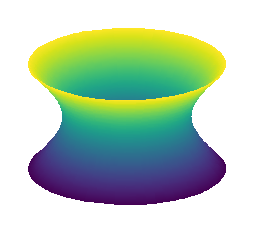
\begin{tikzpicture}[scale=0.5]
            \begin{axis}[
                    view={30}{30},
                    axis lines=none,
                    colormap/viridis,
                    samples=60,
                    domain=-1:1,
                    y domain=-2*pi:2*pi
            ]
            \addplot3[
                    surf,
                    shader=interp,
                    z buffer=sort
            ] ({0.2+cosh(x)*cos(deg(y))},
            {0.2+cosh(x)*sin(deg(y))},
            {sinh(x)});     
            \end{axis}
        \end{tikzpicture}
        \caption{Negative curvature}
     \end{subfigure}
     \hfill
     \begin{subfigure}{0.2\textwidth}
        \centering
        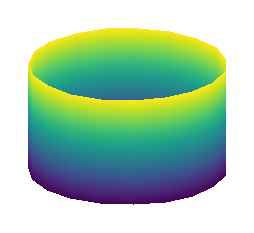
\begin{tikzpicture}[scale=0.5]
            \begin{axis}[
                    view={30}{30},
                    axis lines=none,
                    colormap/viridis,
                    samples=20,
                    domain=0:2*pi,
                    y domain=-1.5:1.5
            ]
            \addplot3[
                    surf,
                    shader=interp,
                    z buffer=sort
            ] ({cos(deg(x))},
            {sin(deg(x))},
            {y});
            \end{axis}
        \end{tikzpicture}
        \caption{Zero curvature.}
     \end{subfigure}
     \hfill
     \begin{subfigure}{0.2\textwidth}
        \centering
        
\begin{tikzpicture}[scale=0.5]
            \begin{axis}[
                    view={30}{0},
                    axis lines=none,
                    colormap/viridis,
                    samples=20,
                    domain=-90:90,
                    y domain=0:360
            ]
            \addplot3[
                    surf,
                    shader=interp,
                    z buffer=sort
            ]
            ({cos(x)*cos(y)},
            {cos(x)*sin(y)},
            {sin(x)});
            \end{axis}
        \end{tikzpicture}
        \caption{Positive curvature}     
    \end{subfigure}
    \label{fig:spaceCurvatures}\
    \caption{Surfaces with various curvatures.}
\end{figure}
Spaces in non-Euclidean geometries can be classified according to their curvature, which measures the deviation from flat Euclidean spaces. Specifically, spaces in elliptic geometry have positive curvature, whilst those in hyperbolic geometry possess negative curvature, as depicted in \Cref{fig:spaceCurvatures}. 

\subsection{Reimannian manifolds}
A Riemannian manifold is a mathematical space that generalizes the concept of curved surfaces and higher-dimensional spaces, allowing us to define distances, angles, and curvature in a smooth way. 

\begin{definition} (Reimannian manifold)
Given a smooth manifold $\Mcal$, a Riemannian metric is a smooth function that assigns to each $p \in \Mcal$ an inner product on the tangent space $\mathcal{T}_p\Mcal$:
\begin{equation*}
    g_p: \mathcal{T}_p\Mcal \times \mathcal{T}_p\Mcal \to \R.
\end{equation*}
    A Reimannian manifold is a pair $(\Mcal,g)$ where $\Mcal$ is a smooth manifold and $g$ is a Riemannian metric.
\end{definition}

Simply put, a \term{manifold} is a topological space\footnote{A \term{topological space} is a set of points, along with a topology, an additional structure which can be defined as a set of neighbourhoods for each point that satisfy some axioms formalizing the concept of closeness.} that locally resembles Euclidean space near each point. More precisely, a $d$-manifold  is a topological space with the property that each point has a neighborhood that resembles an open subset of $d$-dimensional Euclidean space. 

A \term{smooth manifold} is such when functions and coordinate changes along the manifold are infinitely differentiable. The associated metric entails that at each point $p$ lengths and angles are measured differently. 

\paragraph{Distance function and geodesics} An important concept in Euclidean geometry, arising from Euclid's first postulate (\Cref{sec:parallelPostulate}), is that of straight lines, which are shortest paths between points. We can generalize this concept to manifolds by seeking curves with minimal length, called \term{geodesics}. A geodesic is a curve $\gamma(t)=(\gamma(t)^1, \dots, \gamma(t)^d)$ in a manifold $\Mcal$ connecting points $p,q\in \Mcal$ with minimum length. 

In Euclidean space geodesics are straight lines in $\R^d$ and for given parameters $a,b\in \R^d$ they have the form 
\begin{equation}
    \gamma(t) = t\cdot a + b.
\end{equation}

\paragraph{Exponential and logarithmic maps} We would like to associate the points in a manifold to those on a tangent Euclidean space. The tangent space maps to the manifold via an exponential map, and conversely, a logarithmic map translates a point on the manifold to the tangent space. We will see an example of these maps in the following section.

For more details on foundations of manifolds refer to the Appendix in~\cite{Chami2021representationLearningAlgorithmsHyperbolicSpaces}, or~\cite{doCarmo1992riemannianGeometry}\cite{Lee2003smooth}.


\section{Hyperbolic spaces}
Building on the concept of manifolds we analyze how distances and straight lines morph in hyperbolic spaces. In fact, in negative curvature spaces, the space bends like a saddle and triangle angles sum to less than $\pi$. As an example we show a section of a hyperbolic paraboloid (described by function $z=x^2-y^2$) in \Cref{fig:hyperbolicSpace}. In practice it would not be possible to work directly on hyperbolic spaces. Hence, we introduce some ways to operate on hyperbolic spaces and help in their representation. Hyperbolic spaces of constant curvature are difficult to envisage because they cannot be isometrically embedded into any Euclidean space. The reason is, informally, that the former are ``larger'' and have more ``space'' than the latter.  

Because of the fundamental difficulties in representing spaces of constant negative curvature as subsets of Euclidean spaces, there are many equivalent models of hyperbolic spaces\footnote{The possible models of hyperbolic spaces are the following: the Poincaré ball, the Poincaré half-ball, the Klein ball, the hyperboloid model and the upper half-space model.}. Each model emphasizes different aspects of hyperbolic geometry, but no model simultaneously represents all of its properties. In \Cref{sec:hyperboloidModel} we introduce the hyperboloid model as it is useful for computation due to relatively simple formulas for geodesics a. We then focus on Poincaré ball model in \Cref{sec:poincareBall}, that represents the infinite hyperbolic space in a finite ball, and is therefore very useful for visualizations. We then show the relation between these two models (\Cref{sec:isometry}).

For both the models we show how distances are measured and how minimum-length lines are defined. We also put in evidence the respective exponential and logarithmic maps that relate the points on the models to to tangent spaces which are vector spaces that are isomorphic to $\R^d$. In \Cref{hrl} we will use these maps to leverage some of the tools of Euclidean geometry in which standard operations like addition and multiplication are defined for hyperbolic methods, such as optimization or neural network operations.

More in depth discussion on hyperbolic geometry can be found in~\cite{Anderson2006hyperbolicGeometry}\cite{Ramsay2013introductionHyperbolicGeometry}.

\begin{figure}
    \centering
    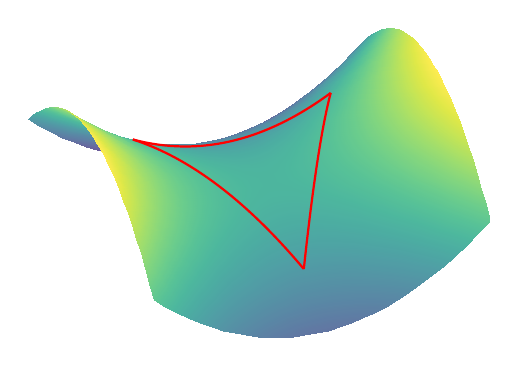
\begin{tikzpicture}
        \begin{axis}[
            view={160}{70},
            colormap/viridis,
            shader=interp,
            axis lines=none,
            xmin=-2, xmax=2,
            ymin=-2, ymax=2,
            zmin=-2, zmax=2,
        ]
        
        % Plot the hyperbolic paraboloid
        \addplot3[
            surf,
            domain=-1.7:1.7,
            domain y=-2:1.5,
            samples=30,
            opacity=0.8,
        ] {x^2 - y^2};
        
        % Define vertices of the triangle (lying on the surface)
        \newcommand{\vertexA}{(-1, -1, 0)}    % z = (-1)^2 - (-1)^2 = 0
        \newcommand{\vertexB}{(1, -1, 0)}     % z = 1^2 - (-1)^2 = 0
        \newcommand{\vertexC}{(0, 1, -1)}     % z = 0^2 - 1^2 = -1
        
        % Edge from A to B (along y = -1, z = x^2 - 1)
        \addplot3[
            thick,
            red,
            smooth,
            samples=50,
            samples y=0,
            domain=-1:1,
        ] ( 
            {x},                % x(x) = -1 → 1
            {-1},               % y(x) = -1 (consxanx)
            {x^2 - 1}         % z(x) = x(t)^2 - y(t)^2 = t^2 - 1
        );
        
        % Edge from A to C (parametric curve)
        \addplot3[
            thick,
            red,
            smooth,
            samples=50,
            samples y=0,
            domain=0:1,
        ] ( 
            {-1 + x},           % x(x) = -1 → 0
           { -1 + 2*x},         % y(x) = -1 → 1
            {(-1 + x)^2 - (-1 + 2*x)^2}  % z(x) = x(t)^2 - y(t)^2
        );
        
        % Edge from B to C (parametric curve)
        \addplot3[
            thick,
            red,
            smooth,
            samples=50,
            samples y=0,
            domain=0:1,
        ] ( 
            {1 - x},            % x(x) = 1 → 0
            {-1 + 2*x},         % y(x) = -1 → 1
            {(1 - x)^2 - (-1 + 2*x)^2}  % z(x) = x(t)^2 - y(t)^2
        );
        \end{axis}
        \end{tikzpicture}

    % 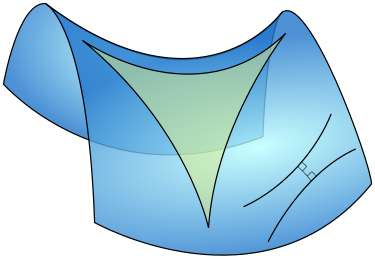
\includegraphics[width=0.3\textwidth]{figs/Hyperbolic_triangle.png}    
    \caption{Section of a hyperbolic space.}
    \label{fig:hyperbolicSpace}
\end{figure}




\subsection{Hyperboloid model}\label{sec:hyperboloidModel}
We first introduce some useful quantities for our discussion.

\begin{definition}(Minkowski inner product) \label{def:minkowskiInnerProduct}
    Given two vectors $x,y \in \R^d$, their Minkowski inner product is defined as:
    \begin{equation*}
        \langle x, y \rangle_\Lcal = -x_0y_0+\sum_{i=1}^d x_iy_i
    \end{equation*}    
\end{definition}

\begin{definition}(Minkowski norm) \label{def:minkowskiNorm}
    Given a vector $x \in \R^d$, its Minkowski norm is defined as:
    \begin{equation*}
        \|x\|_\Lcal = \sqrt{\langle x, x \rangle_\Lcal}.
    \end{equation*}
\end{definition}

We can now define the hyperboloid model of hyperbolic space.
\begin{definition}[Hyperbolic model]
    We denote $\Hy^{d,\kappa}$ as the hyperboloid manifold in $d$ dimension with constant negative curvature $\frac{1}{\kappa}$ with $\kappa>0$ as
    \begin{equation*}
        \Hy^{d,\kappa} = \left\{x \in \R^{d+1} : \langle x, x \rangle_\Lcal = -\kappa, x_0 > 0\right\}
    \end{equation*}
\end{definition}

\begin{figure}
    \begin{subfigure}{0.48\textwidth}
        \centering
        \begin{tikzpicture}[scale=1.7]
            \draw (0,0) circle (1);
            \clip (0,0) circle (1);
            \hgline{30}{-30}{black!70}
            \hgline{180}{270}{blue!20}
            \hgline{30}{120}{black!70}
            \hgline{0}{180}{red!50}
        \end{tikzpicture}
        \caption{Poincaré ball model.}
        \label{fig:poincareBall}
    \end{subfigure}%
    \hfill
    \begin{subfigure}{0.48\textwidth}
        \centering
        \begin{tikzpicture}
        \begin{axis}[
            view={30}{10},
            colormap name=custom,
            shader=interp,
            axis lines=none,
            xmin=-3, xmax=3,
            ymin=-3, ymax=3,
            zmin=0, zmax=5,
        ]
        \addplot3[
            surf,
            domain=-2.8:2.8,
            y domain=-2.8:2.8,
            samples=20,
            z buffer=sort,
            opacity=0.7
        ] {sqrt(x^2 + y^2 + 1)};
        \end{axis}
        \end{tikzpicture}   
        \caption{Hyperboloid model.}
        \label{fig:hyperboloid}
    \end{subfigure}
    \caption{Models of hyperbolic space.}
    \label{fig:hyperbolicmodels}
\end{figure}


For each point $p$ in a hyperboloid $\Hy^{d,\kappa}$ the tangent space at $p$---$\mathcal{T}_p\Hy$---is a $d$-dimensional vector space containing all possible directions of paths leaving from $p$. 
Formally the tangent space to point $p$ is defined as:
\begin{align}\label{eq:tangentSpace}
    \mathcal{T}_p\Hy^{d,\kappa} 
    &= \left\{u\in \R^{d+1} : \langle u, p \rangle_\Lcal = 0\right\} \\
    &= \left\{(v_0,v) \in \R^{d+1} : v_0 = \frac{v \cdot p}{\sqrt{\kappa(1 + \|p\|^2_2)}}\right\}
\end{align}

From hereon we refer to a hyperboloid model with negative curvature $1$ ($\Hy^{d,1}$), that we simply indicate with $\Hy^d$. In two dimensions the hyperboloid can be visualized as a surface in $\R^3$ which corresponds to the upper sheet of a two sheet hyperboloid of revolution (\Cref{fig:hyperboloid}).

\paragraph{Distance function and geodesics}
Let $p\in\Hy^d$ and $v\in \mathcal{T}_p\Hy^d$, assuming $\langle v,v\rangle_\Lcal $ = 1. In the hyperboloid model the unique geodesic $\gamma_{p,v}(\cdot)$ such that $\gamma_{p,v}(0)=p$ and $\dot{\gamma}_{p,v}(0)=v$ is given by:

\begin{equation*}
    \gamma_{p,v}(t) = \cosh(t)p + \sinh(t)v.
\end{equation*}

The corresponding intrinsic distance\footnote{An \term{intrinsic distance} refers to the shortest path between two points measured \emph{within} a given space or surface, rather than through an external surrounding space.} between two points $p,q\in\Hy^d$ can be computed as:

\begin{equation}\label{eq:distance_hyperboloid}
    d_{\Hy^d}(p, q) = \text{arcosh}(-\langle p, q \rangle_\Lcal).
\end{equation}

\paragraph{Exponential and logarithmic maps}
When dealing with the hyperboloid model, given $p \in \Hy^d$ and a tangent vector $v \in \mathcal{T}_p\Hy^d$, the exponential map $\exp_p: \mathcal{T}_p\Hy^d \to \Hy^d$ assigns to $v$ the point $\exp_p(v) := \gamma(1)$, where $\gamma$ is the unique geodesic satisfying $\gamma(0) = p$ and $\dot{\gamma}(0) = v$. The logarithmic map $\log_p: \Hy^d \to \mathcal{T}_pHy^d$ reverses back to the tangent space at $p$ such that $\log_p(\exp_p(v)) = v$. In hyperbolic spaces these operations form a bijection between the entire hyperbolic space and the tangent space at a point. The analytic expressions for the exponential and logarithmic maps are given below, under the assumption that $v\neq 0$.

\begin{align}
    \exp_p(v) &= \cosh(\|v\|_\Lcal)p + \sinh(\|v\|_\Lcal) \frac{v}{\|v\|_\Lcal} \label{eq:log_hyperboloid}\\
    \log_p(y) &= d_{\Lcal}(p,y)\frac{y + \langle p,y \rangle_{\Lcal}p}{\|y + \langle p,y \rangle_{\Lcal}p\|_{\Lcal}} \label{eq:exp_hyperboloid}
\end{align}

\subsection{Poincaré ball model}\label{sec:poincareBall}
Poincaré's representation of hyperbolic geometry is based on the points in the unit ball in $d$ dimensions, formally described as
\begin{equation*}
    \B^d = \{x \in \R^d: \|x\|^2_2 < 1\}.
\end{equation*}
The boundary of the ball is not a part of the hyperbolic plane it represents, but represents its infinitely remote points, called \term{boundary at infinity}.

We now use the mathematical framework called \term{gyrovector spaces}~\cite{ungar2022gyrovectorSpaceHyperbolicGeometry}\cite{Ungar1999HyperbolicPythagoreanTheoremPoincareDiscModel} to describe elementary operations such as additions and scalar multiplications in the Poincaré ball model in analogy with Euclidean geometry.

Vector addition is not well-defined in the Poincaré ball, since adding two points might result in a point outside the ball. Instead, Möbius addition provides an analogue to Euclidean addition for hyperbolic space. We define the Möbius addition in the Poincaré ball model.

\begin{definition}[Möbius addition]
    Given two points $p,q\in\B^d$, the Möbius addition is defined as:
    \begin{equation*}
        p \oplus q = \frac{(1 +  2\langle p,q\rangle_2 + \|q\|^2_2)}{(1 + 2\langle p,q\rangle_2 + \|p\|^2_2\|q\|^2_2)}.
    \end{equation*}
    
\end{definition}

In contrast to Euclidean addition, it is neither commutative nor associative. However, it provides an analogue through the lens of the parallel transport concept. Given two points $x,y$ and a tangent vector $v$ in $\mathcal{T}_x$, there is a unique tangent vector in $\mathcal{T}_y$ which creates the same angle as $v$ with the direction of the geodesic connecting $x$ and $y$. This is called the \term{parallel transport} $P_{x\to y} (v)$ of $v$ along the geodesic from $x$ to $y$. In Euclidean geometry parallel transport is the standard Euclidean addition. Analagously, the Möbius addition satisfies the following property:
\begin{equation*}
    p\oplus q=\exp_{x}(P_{o\to x}(\log_o(q))).
\end{equation*}

Similarly, the Möbius scalar multiplication provides a way to scale points on a manifold by a scalar. In the case of the Poincaré ball it is defined as follows.

\begin{definition}[Möbius scalar multiplication]
    Given a point $p\in\B^d$ and a scalar $\alpha\in\R$, the Möbius scalar multiplication is defined as:
    \begin{equation*}
        \alpha \otimes p = \tanh({\alpha \tanh^{-1}(\|p\|_2)})\frac{p}{\|p\|^2_2}.
    \end{equation*}
\end{definition}

\paragraph{Distance function and geodesics}
When the unit ball is endowed with the family of inner products
\begin{equation*}
    g_p = \left(\frac{2}{1-\|p\|^2_2}\right)^2\mathbb{I}_d,
\end{equation*}
the pair $(\B^d,g)$ forms a Riemannian manifold of constant negative curvature. The induced distance between two points $p,q$ in $\B^d$ can be found through
\begin{align}\label{eq:poincareDistance}
    d_\B(p,q) &= \text{arcosh}\left(1 + 2\frac{\|p-q\|^2_2}{(1-\|p\|^2_2)(1-\|q\|^2_2)}\right)\\
              &= 2\text{arctanh}(\|-p\oplus q\|).
\end{align}

This yields geodesics that are either straight lines that go through the origin of the ball, or segments of circles that are perpendicular to the boundary of the ball as shown in \Cref{fig:hyperbolicmodels}. Using Möbius addition and scalar multiplication we can determine the geodesic between two points $p,q\in\B^d$ as follows:
\begin{equation*}
    \gamma_{p,q}(t) = p\oplus (-p \oplus y) \otimes t.
\end{equation*}

\paragraph{Exponential and logarithmic maps}\label{sec:expLogMaps_poincareBall}
Like for the hyperboloid model there exist analytical expressions that define the exponential and logarithmic maps in a given point $p$ lying on $\B^d$ and on the tangent space in that point $\mathcal{T}_p\B^d$. 

\begin{align}
    \exp_p(v) &= p \oplus \left(\tanh\left(\frac{\lambda_p\|v\|_2}{2}\right)\frac{v}{\|v\|_2}\right) \label{eq:exp_poincareBall} \\
    \log_p(y) &= \frac{2}{\lambda_p}\text{arctan}(\|-p \oplus y\|_2)\frac{-p \oplus y}{\|-p \oplus y\|_2} \label{eq:log_poincareBall}
\end{align}

where $\lambda_p$ is a curvature-dependent conformal factor at $p$.

\begin{figure}
  \centering
  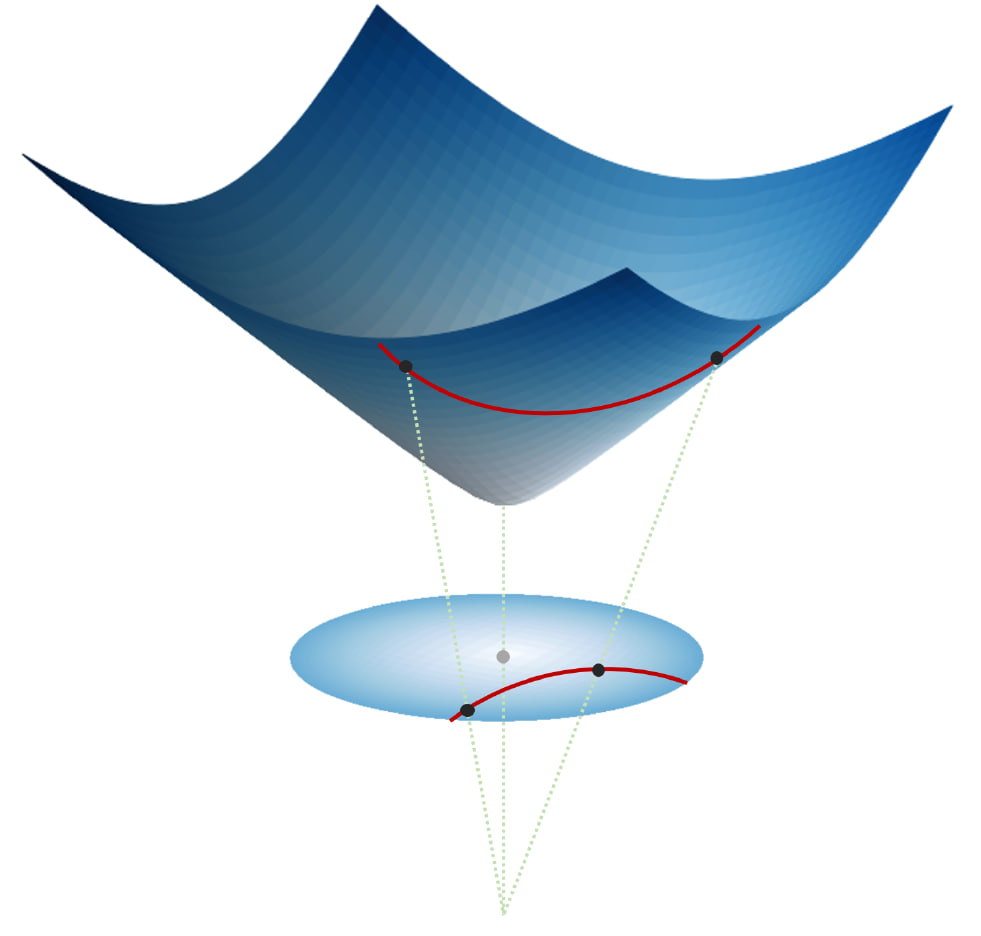
\includegraphics[width=0.5\textwidth]{figs/hyperboloidToPoincare.jpg}

    % \begin{tikzpicture}
    %     \begin{axis}[view={30}{20},axis lines=none]
    %       % Draw the hyperboloid
    %       \addplot3[surf, shader=interp, colormap/blackwhite, domain=-2:2]
    %         {x^2+y^2+1};
        
    %     % Limit geodesic curve to fit within the drawn hyperboloid
    %     \addplot3[domain=-0.9:1.63,samples=50, samples y=0, thick, blue]
    %     {sqrt(sinh(x)^2 + cosh(x)^2 + 1)+1};

        
          
    %     \end{axis}


    %   \end{tikzpicture}
  \caption{Illustration of the hyperboloid (top) and its connection to the Poincaré disk (bottom)\cite{Chami2021representationLearningAlgorithmsHyperbolicSpaces}.}
  \label{fig:hyperboloidToPoincareBall}
\end{figure}

\subsection{Isometry between hyperboloid and Poincaré ball}\label{sec:isometry}
The Poincaré ball model of hyperbolic space is isomorphic\footnote{An \term{isomorphism} is a bijective mapping between two structures that preserves their operations, relationships and properties.} to the hyperboloid model, as show in \Cref{fig:hyperboloidToPoincareBall}. The stereographic projection\footnote{The \term{stereographic projection} is a mapping that projects a sphere (space) onto a plane, preserving shapes locally.}
\begin{equation}\label{eq:stereographicProjection}
    (x_0, x_1, \ldots, x_d) \mapsto \left(\frac{x_1, \ldots, {x_d}}{1+x_0}\right)
\end{equation}
is an isometry between $\Hy^{d}$ and the Poincaré ball $\B^{d+1}$. Its inverse map is given by
\begin{equation}\label{eq:inverseStereographicProjection}
    (y_1, \ldots, y_d) \mapsto \left(\frac{1 + \|y\|^2, 2y_1, \ldots, 2y_d}{1 - \|y\|^2}\right).
\end{equation}

\section{Connections between hyperbolic spaces and trees}\label{sec:hyperbolicAndTrees}
We now discuss the connections between hyperbolic spaces and tree-like structures, that explain the use of hyperbolic spaces to represent hierarchical data, as we will discuss in \Cref{hrl}. Various studies have shown that many real-world networks exhibit hierarchical structures with underlying hyperbolic geometry~\cite{Krioukov2010HyperbolicGeometryComplexNetworks}\cite{Papadopoulos2012popularityVSSimilarityGrowingNetworks}. We explore this relation theoretically by correlating hyperbolic metrics and tree metrics (\Cref{sec:hyperbolicTreeMetrics}), and more intuitively looking at the structure of trees (\Cref{sec:expGrowth}).

\subsection{Hyperbolic and tree metrics}\label{sec:hyperbolicTreeMetrics}
To identify tree-like structures we turn to notion of Gromov $\delta$-hyperbolicity~\cite{gromov1987hyperbolic}\cite{adcock2013tree}\cite{chen2013hyperbolicity}. To define $\delta$-hyperbolic spaces we introduce the Gromov product~\cite{gromov1987hyperbolic}. This quantity measures how close two points are to each other relative to a third point.  

\begin{definition}[Gromov product]
    In any metric space $(X,d)$, the Gromov product of two points $x,y\in X$ with respect to a third point $z\in X$ is defined as:
    \begin{equation*}
        \langle x,y \rangle_z = \frac{1}{2}\left(d(x,z) + d(y,z) - d(x,y)\right).
    \end{equation*}
\end{definition}

\begin{definition}[$\delta$-hyperbolicity, four-point condition]
    A metric space $(X,d)$ is $\delta$-hyperbolic if there exists $\delta\geq0$ such that for all $x,y,z,w\in X$
    \begin{equation*}
        \langle x,y\rangle_z \geq \min\{\langle x,w\rangle_z, \langle y, w\rangle_z\} - \delta.
    \end{equation*}
\end{definition}

We use a metric describing distances in trees as a baseline to compare metric spaces' $\delta$-hyperbolicities.

\begin{definition}[Metric tree]
    A metric space $(X,d)$ is a metric tree if there exists a tree $T=(X,E_T)$ with edges in $E_T$ such that for $u,v\in X$ it holds that $d(u,v)=d_T(u,v)$
\end{definition}
where $d_T(u,v)$ is the length of the shortest path between $u$ and $v$ in the tree $T$. 
 
\begin{figure}
    \centering
    \begin{tikzpicture}
        \node at (0,-1) [circle, draw, fill=black, inner sep=1pt] (z) {};
        \node at (0,-1.7) [circle, draw, fill=black, inner sep=1pt] (a) {};
        \node at (0,-2.4) [circle, draw, fill=black, inner sep=1pt] (b) {};
        \node at (-0.7,-3) [circle, draw, fill=black, inner sep=1pt]  (x) {};
        \node at (0.7,-3) [circle, draw, fill=black, inner sep=1pt] (c) {};
        \node at (1.4,-3.6) [circle, draw, fill=black, inner sep=1pt] (y) {};

        \draw[thick] (z) -- (a);
        \draw[thick] (a) -- (b);
        \draw[thick] (b) -- (x);
        \draw[thick] (b) -- (c);
        \draw[thick] (c) -- (y);

        \draw [decorate,decoration={brace,amplitude=8pt,mirror}] (b) -- (z) node[midway,xshift=10pt,right]{\footnotesize $\langle x,y\rangle_z$};


        \node[left=0.1cm of z] {$z$};
        \node[left=0.1cm of x] {$x$};
        \node[right=0.1cm of y] {$y$};
        

    \end{tikzpicture}
    \caption{Interpretation of the Gromov product in a simple tree.}
    \label{fig:slimTriangle}
\end{figure}


\begin{figure}
    \begin{subfigure}{0.25\textwidth}
        \centering
        \begin{tikzpicture}
            \node at (0,1) [circle, draw, fill=black, inner sep=0.5pt] (z) {};
            \node at (-0.866,-0.5) [circle, draw, fill=black, inner sep=0.5pt]  (x) {};
            \node at (0.866,-0.5) [circle, draw, fill=black, inner sep=0.5pt] (y){};

            
            \draw (z) -- (x);
            \draw (y) -- (x);
            \draw (z) -- (y);

            \clip (0,0) circle (1);
        \end{tikzpicture}
        \caption{In a Euclidean space.}
    \end{subfigure}
    \hfill
    \begin{subfigure}{0.25\textwidth}
        \centering
        \begin{tikzpicture}
            \node at (0,1) [circle, draw, fill=black, inner sep=0.5pt] (z) {};
            \node at (-0.866,-0.5) [circle, draw, fill=black, inner sep=0.5pt] (x) {};
            \node at (0.866,-0.5) [circle, draw, fill=black, inner sep=0.5pt] (y) {};
                        
            \clip (0,0) circle (1);
            \hgline{90}{-30}{black};
            \hgline{-150}{-30}{black};
            \hgline{210}{90}{black};

        \end{tikzpicture}
        \caption{In a hyperbolic space.}
    \end{subfigure}
    \hfill
    \begin{subfigure}{0.25\textwidth}
        \centering
        \begin{tikzpicture}
            \node at (0,1) [circle, draw, fill=black, inner sep=0.5pt] (z) {};
            \node at (0,0.2) [circle, draw, fill=black, inner sep=0.01pt] (b) {};           
            \node at (-0.866,-0.5) [circle, draw, fill=black, inner sep=0.5pt]  (x) {};
            \node at (0.866,-0.5) [circle, draw, fill=black, inner sep=0.5pt] (y){};
            
            \draw (z) -- (b);
            \draw (b) -- (x);
            \draw (b) -- (y);

            \clip (0,0) circle (1);
        \end{tikzpicture}
        \caption{In a tree space.}
    \end{subfigure}
    \caption{Triangles in various metric spaces.}
    \label{fig:triangles}
\end{figure}
One can show that metric trees are $0$-hyperbolic. Let $(X,d)$ be a metric tree, then $\langle x, y\rangle_z$ is the maximum number of edges in $T=(X,E_T)$ between the node $z$ and a common parent for $x$ and $y$ (\Cref{fig:slimTriangle}). It follows that for $x,y,w\in X$ it holds that $\langle x,y\rangle_z \geq \min\{\langle x,w\rangle_z, \langle y, w\rangle_z\}$. Therefore, metric spaces with smaller $\delta$ will be closer to a tree metric. One can show that the Euclidean space is not $\delta$-hyperbolic, whilst hyperbolic spaces are $\log 3$-hyperbolic in the sense of Gromov. This can be noticed by observing triangles in a Euclidean, a hyperbolic and a tree metric (\Cref{fig:triangles}). Indeed we see that with lower $\delta$-hyperbolicity of the metric space, the distance between two vertices increasingly approaches the distance to the ``centre'' of the triangle.

There are important properties such as quasi-isometries between $\delta$-hyperbolic spaces and tree metric spaces. We formalize that any finite set of points in a $\delta$-hyperbolic space can be embedded in a tree metric with bounded distortion~\cite{gromov1987hyperbolic}.

\begin{proposition}[Tree-likeliness of hyperbolic space]
    There is a constant $C_n =\delta \cdot O(n)$ such that for any set of points $x_1, x_2, \dots,x_n$ in a $\delta$-hyperbolic space $(\Mcal,d_\Mcal)$ can be embedded via $f:\Mcal \to T$ into a tree metric $(T,d_T)$ such that:
    \begin{equation*}
        d_\Mcal(x_i, x_j)\leq d_T(f(x_i), f(x_j)) \leq d_\Mcal(x_i, x_j) + C_n.
    \end{equation*}
\end{proposition}

More specifically, Sarkar~\cite{sarkar2011lowDIstortionDelaunayEmbedding} derived a construction to embed trees in hyperbolic spaces with arbitrarily low-distortion in two dimensions.

\begin{proposition}[Sarkar]
    Any tree $T=(X,E_T)$ can be embedded into $(\mathbb{B}^2, d_\mathbb{B})$ with scale $\zeta = O(1/\varepsilon)$ and worst-case distortion at most $1 + \varepsilon$.
\end{proposition}

These nice quasi-isometries between hyperbolic spaces and tree metric spaces justify the use of hyperbolic geometry to embed tree-like graphs with low distortion. Since we have these quasi-isometric mappings, hyperbolic spaces can be thought of as some continuous version of trees. We will leverage these properties in the next chapter. 

\subsection{Exponential volume growth}\label{sec:expGrowth}
As we have concluded in the previous section, trees can be thought of as the discrete approximation of some underlying hyperbolic space, where geodesics resemble shortest paths in discrete trees. One can define a notion of volume in trees as the number of nodes contained within some bounded distance (the radius) to the root of the tree. This volume grows exponentially as we increase the radius, as shown in \Cref{fig:radialTree}.

\tikzset{level 1/.style={sibling angle=60,level distance=32mm}}
\tikzset{level 2/.style={sibling angle=35,level distance=16mm}}
\tikzset{level 3/.style={sibling angle=20,level distance=8mm}}
\tikzset{every node/.style={circle, fill=black, inner sep=0pt, color=black}}
\tikzset{edge from parent/.style={segment angle=10,draw}}


\begin{figure}
    \centering
    \begin{tikzpicture}
    [grow cyclic, scale=0.35]
    \node {} 
    child  foreach \A in {1,1,1,1,1,1}{  
    node{} 
        child foreach \B in {2,2,2}{ 
        node {} 
            child foreach \C in {3,3,3}{
            node {} }
        }
    };
    \end{tikzpicture}
    \caption{Volume growth in trees.}
    \label{fig:radialTree}
\end{figure}


In Euclidean space the volume of balls grows polynomially with the radius, making it less suitable to represent exponentially growing graphs like trees. More concretely, because the growth is not as fast as that of the graph, the Euclidean space quickly becomes too crowded, resulting in geodesics intersecting each other.

In contrast, $\delta$-hyperbolic spaces, and in particular hyperbolic spaces, have exponential growth. For instance, in a two dimensional hyperbolic space with constant curvature $\kappa = -1$, the length of a circle is given as $2\pi \sinh r$ while the area of a ball is given as $2\pi(\cosh r - 1)$. Since $\sinh r = \frac{1}{2} (e^r - e^{-r})$ and $\cosh r = \frac{1}{2} (e^r + e^{-r})$, both disc area and circle length grow exponentially with $r$. 

This feature yields more room to fit complex hierarchies and makes these spaces ideal candidates to embed trees while accommodating for their exponential volume growth. 
\part*{Our contribution}
\chapter{Experiments}
We now engage in our contribution to tackling the issue of automatic differential diagnosis of Mendelian diseases. In this context, we have developed a customized knowledge graph (KG) integrated with patient data, which we detail in \Cref{sec:patientKG}. Furthermore, we outline the methodology by which we have reformulated our problem as a link prediction task, demonstrating the validity of our selection of hyperbolic graph representation learning techniques (\Cref{sec:linkPredictionDiffDiagnosis}).

\section{Patient KG}\label{sec:patientKG}
In this section, we delineate the data selected for the purpose of differential diagnosis of Mendelian diseases. We proceed with an exploration of the underlying biomedical knowledge graph utilized and the patient data chosen. Additionally, we describe how these data sources have been integrated into a singular knowledge graph.

\subsection{Underlying biomedical KG}\label{sec:underlyingKG}
Initially, we considered PrimeKG \cite{chandak2023PrimeKG}, a knowledge graph aimed at precision medicine analyses that aggregates 20 high-quality resources. Unfortunately, at the time of use, we encountered significant shortcomings regarding the representation of Mendelian diseases. Drawing inspiration from the entities represented in PrimeKG, we constructed a customized knowledge graph. We have resorted to \emph{PheKnowLator} (\emph{Phenotype Knowledge Translator})~\cite{callahan2020PheKnowlator}\footnote{The Python library is accessible at \url{https://github.com/callahantiff/PheKnowLator}}, a KG framework designed for optimized construction of semantically rich, large-scale biomedical KGs that accommodates various standardized terminologies or vocabularies. To build our heterogeneous graph, we selected various ontologies, taking into account our final objectives and memory constraints. The chosen ontologies, categorized by resulting node types, are outlined below.

\begin{multicols}{2}

\paragraph{Gene Ontology}
\begin{itemize}
\item Gene Ontology Chemical Entities (GOCHE)
\item Gene Ontology (GO)
\end{itemize}

\paragraph{Genomic Features}
\begin{itemize}
\item Ontology of Genes and Genomes (OGG)
\item Sequence Ontology (SO)
\end{itemize}

\paragraph{Proteins}
\begin{itemize}
\item Protein Ontology (PR)
\item Cell Ontology (CL)
\item Human Phenotype Ontology (HP)
\item Molecular Function (MF)
\end{itemize}
\bigskip

\paragraph{Diseases}
\begin{itemize}
\item Disease Ontology (DOID)
\item Mondo Disease Ontology (MONDO)
\end{itemize}
\bigskip

\paragraph{Phenotypes}
\begin{itemize}
\item Human Phenotype Ontology (HP)
\item Phenotype And Trait Ontology (PATO)
\item uPheno Ontology (UPHENO)
\end{itemize}
\end{multicols}
\begin{table}
    \centering
    \begin{tabular}{rr}
        \toprule
        \textbf{Node Type} & \textbf{\#} \\
        \midrule
        Protein & 122,740 \\
        GO & 40,803 \\
        Disease & 26,899 \\
        Genomic feature & 24,031 \\
        Phenotype & 19,645 \\
        \bottomrule
    \end{tabular}
    \caption{Distribution of node types in the knowledge graph}
    
    \label{tab:nodetypes}
\end{table}
\begin{table}
    \centering
    \begin{tabular}{lllr}
        \toprule
        \textbf{Edge Predicate} & \textbf{Subject} & \textbf{Object} & \textbf{\#} \\      
        \midrule
        Molecularly interacts with & Protein & Protein & 618,856 \\
        Phenotype of & Disease & Phenotype & 453,260 \\
        Has phenotype & Phenotype & Disease & 453,260 \\
        Subclassof & Protein & Protein & 164,224 \\
        Has participant & Protein & GO & 125,233 \\
        Participates in & GO & Protein & 125,230 \\
        Located in & GO & Protein & 81,468 \\
        Subclassof & GO & GO & 81,608 \\
        Location of & Protein & GO & 81,466 \\
        Has function & GO & Protein & 68,742 \\
        Function of & Protein & GO & 68,742 \\
        Subclassof & Disease & Disease & 45,251 \\
        Subclassof & Genomic feature & Genomic feature & 28,130 \\
        Subclassof & Phenotype & Phenotype & 25,852 \\
        Causes/contributes to condition & Phenotype & Genomic feature & 24,519 \\
        Has gene template & Genomic feature & Protein & 20,089 \\
        Gene product of & Genomic feature & Protein & 19,607 \\
        Has gene product & Protein & Genomic feature & 19,607 \\
        Causes/contributes to condition & Disease & Genomic feature & 14,418 \\
        Part of & GO & GO & 6,772 \\
        \bottomrule
    \end{tabular} 
    \caption{Distribution of (frequent) edge predicates per node type in the knowledge graph}   
    \label{tab:edgedistrib}
\end{table}
\begin{figure}
    \centering
    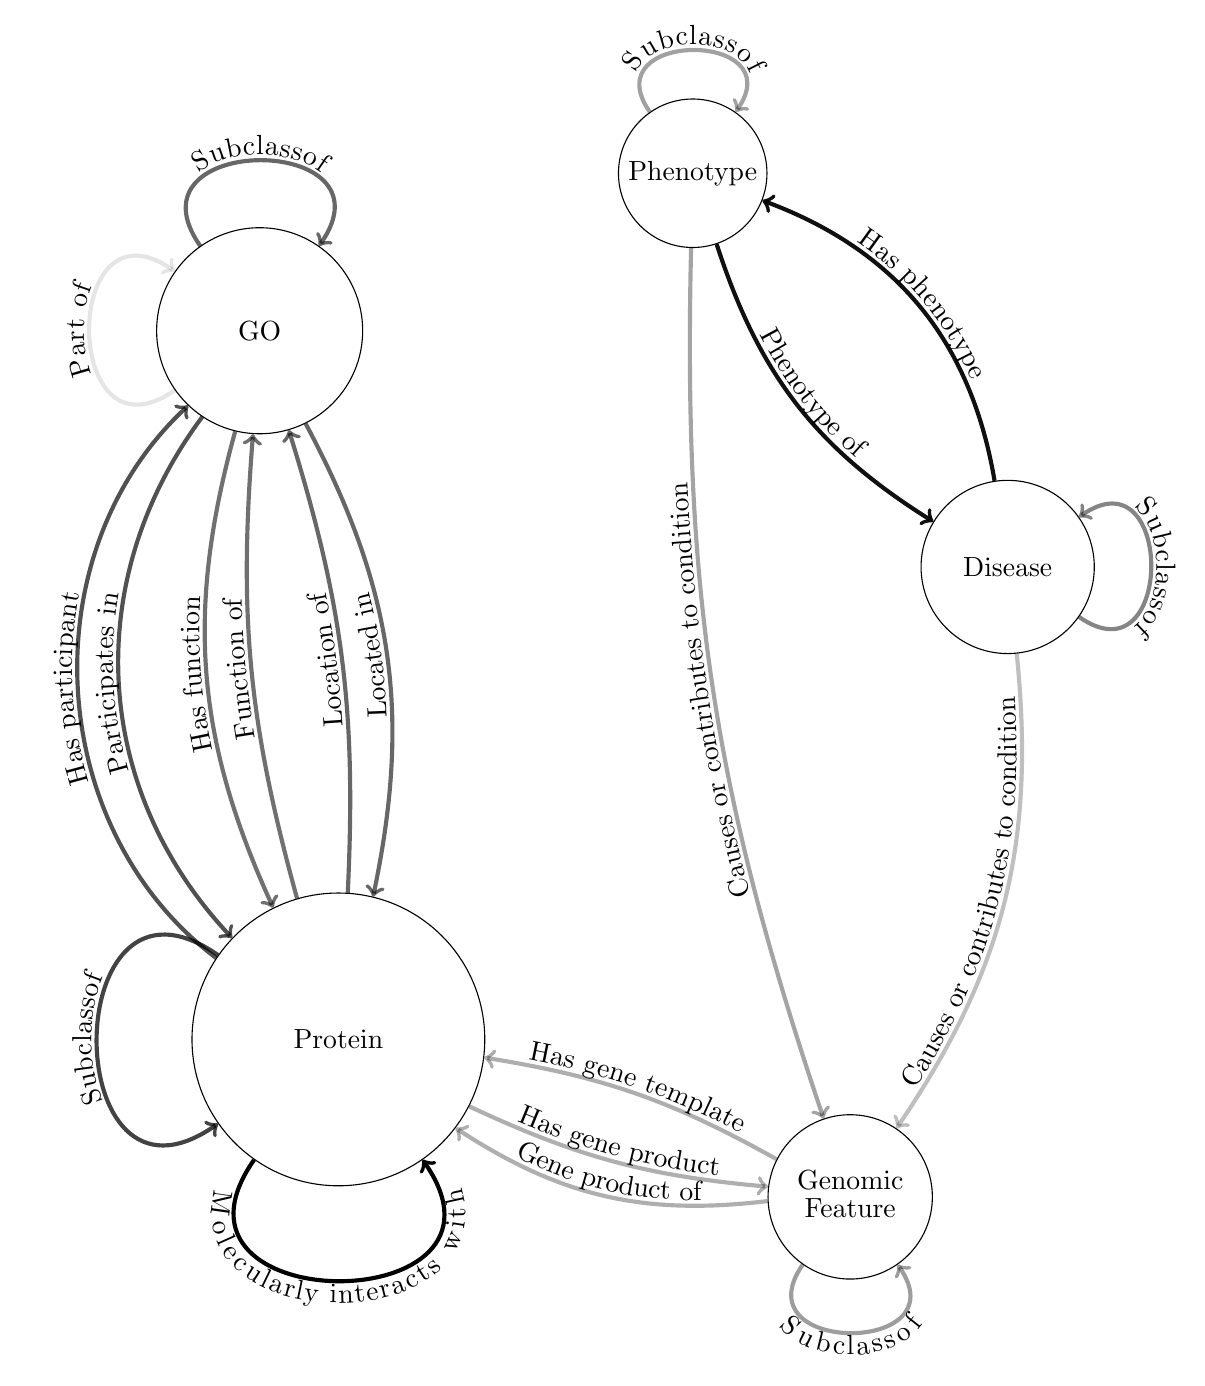
\begin{tikzpicture}
    \usetikzlibrary{decorations.text}

    \begin{scope}[xshift=1cm]
        % Nodes
        \node[circle, draw, fill=none, minimum size=3.718cm, inner sep=0pt] (Protein) at (-4,-3) {Protein};
        \node[circle, draw, fill=none, minimum size=2.617cm, inner sep=0pt] (GO) at (-5,6) {GO};
        \node[circle, draw, fill=none, minimum size=2.200cm, inner sep=0pt] (Disease) at (4.5,3) {Disease};
        \node[circle, draw, fill=none, minimum size=2.087cm, inner sep=0pt] (GenomicFeature) at (2.5,-5) {\begin{tabular}{c}Genomic\\[-0.5ex]Feature\end{tabular}};
        \node[circle, draw, fill=none, minimum size=1.886cm, inner sep=0pt] (Phenotype) at (0.5,8) {Phenotype};

        % Edges with curved labels
            \draw[->, line width=1.5pt, opacity=0.937927] (Disease) to[bend right=30] (Phenotype);
            \path[decorate, decoration={text along path, text align=center, raise=2pt, text={Has phenotype}}] (Phenotype) to[bend left=30] (Disease);

            \draw[->, line width=1.5pt, opacity=1.000000] (Protein) to[out=235, in=305, looseness=3] (Protein);
            \path[decorate, decoration={text along path, text align=center, raise=-8pt, text={Molecularly interacts with}}] (Protein) to[out=235, in=305, looseness=3](Protein);

            \draw[->, line width=1.5pt, opacity=0.478617] (Disease) to[out=-35, in=35, looseness=3] (Disease);
            \path[decorate, decoration={text along path, text align=center, raise=2pt, text={Subclassof}}] (Disease) to[out=35, in=-35, looseness=3] (Disease);

            \draw[->, line width=1.5pt, opacity=0.596164] (GO) to[out=125, in=55, looseness=3] (GO);
            \path[decorate, decoration={text along path, text align=center, raise=2pt, text={Subclassof}}] (GO) to[out=125, in=55, looseness=3] (GO);

            \draw[->, line width=1.5pt, opacity=0.383857] (GenomicFeature) to[out=235, in=305, looseness=3] (GenomicFeature);
            \path[decorate, decoration={text along path, text align=center, raise=-8pt, text={Subclassof}}] (GenomicFeature) to[out=235, in=305, looseness=3] (GenomicFeature);

            \draw[->, line width=1.5pt, opacity=0.367024] (Phenotype) to[out=125, in=55, looseness=3] (Phenotype);
            \path[decorate, decoration={text along path, text align=center, raise=2pt, text={Subclassof}}] (Phenotype) to[out=125, in=55, looseness=3] (Phenotype);

            \draw[->, line width=1.5pt, opacity=0.735558] (Protein) to[out=145, in=215, looseness=3] (Protein);
            \path[decorate, decoration={text along path, text align=center, raise=2pt, text={Subclassof}}] (Protein) to[out=215, in=145, looseness=3] (Protein);

            \draw[->, line width=1.5pt, opacity=0.561965] (Protein) to[bend left=10] (GO);
            \path[decorate, decoration={text along path, text align=center, raise=2pt, text={Function of}}] (Protein) to[bend left=10] (GO);


            \draw[->, line width=1.5pt, opacity=0.937927] (Phenotype) to[bend right=20] (Disease);
            \path[decorate, decoration={text along path, text align=center, raise=2pt, text={Phenotype of}}] (Phenotype) to[bend right=20] (Disease);

            \draw[->, line width=1.5pt, opacity=0.316749] (GenomicFeature) to[bend right=10] (Protein);
            \path[decorate, decoration={text along path, text align=center, raise=2pt, text={Has gene template}}] (Protein) to[bend left=10] (GenomicFeature);

            \draw[->, line width=1.5pt, opacity=0.561965] (GO) to[bend right=20] (Protein);
            \path[decorate, decoration={text along path, text align=center, raise=2pt, text={Has function}}] (Protein) to[bend left=20] (GO);

            \draw[->, line width=1.5pt, opacity=0.681528] (Protein) to[bend left=50] (GO);
            \path[decorate, decoration={text along path, text align=center, raise=2pt, text={Has participant}}] (Protein) to[bend left=50] (GO);

            \draw[->, line width=1.5pt, opacity=0.311908] (Protein) to[bend right=10] (GenomicFeature);
            \path[decorate, decoration={text along path, text align=center, raise=2pt, text={Has gene product}}] (Protein) to[bend right=10] (GenomicFeature);

           

            \draw[->, line width=1.5pt, opacity=0.595817] (Protein) to[bend right=10] (GO);
            \path[decorate, decoration={text along path, text align=center, raise=2pt, text={Location of}}] (Protein) to[bend right=10] (GO);

            \draw[->, line width=1.5pt, opacity=0.595822] (GO) to[bend left=20] (Protein);
            \path[decorate, decoration={text along path, text align=center, raise=2pt, text={Located in}}] (Protein) to[bend right=20] (GO);

            \draw[->, line width=1.5pt, opacity=0.681523] (GO) to[bend right=40] (Protein);
            \path[decorate, decoration={text along path, text align=center, raise=2pt, text={Participates in}}] (Protein) to[bend left=40] (GO);

            \draw[->, line width=1.5pt, opacity=0.250632] (Disease) to[bend left=20] (GenomicFeature);
            \path[decorate, decoration={text along path, text align=center, raise=2pt, text={Causes or contributes to condition}}] (GenomicFeature) to[bend right=20] (Disease);

            \draw[->, line width=1.5pt, opacity=0.356471] (Phenotype) to[bend right=10] (GenomicFeature);
            \path[decorate, decoration={text along path, text align=center, raise=2pt, text={Causes or contributes to condition}}] (GenomicFeature) to[bend left=10] (Phenotype);

            \draw[->, line width=1.5pt, opacity=0.311908] (GenomicFeature) to[bend left=20] (Protein);
            \path[decorate, decoration={text along path, text align=center, raise=2pt, text={Gene product of}}] (Protein) to[bend right=20] (GenomicFeature);

            \draw[->, line width=1.5pt, opacity=0.100000] (GO) to[out=215, in=145, looseness=3] (GO);
            \path[decorate, decoration={text along path, text align=center, raise=2pt, text={Part of}}] (GO) to[out=215, in=145, looseness=3] (GO);   \end{scope}
    \end{tikzpicture}

    \caption{A hypergraph representation of the underlying knowledge graph, having hypernodes representing the possibile node types and hyperedges for the most frequent edge predicates. The hypernodes' size and the hyperedges' opacity are logarithmic in the amount of node types and edge predicates respectively.}
    \label{fig:kg_hypergraph}
\end{figure}
The relations between the entities and their predicates derive from the annotations specified in the ontologies.

In terms of magnitude, the knowledge graph comprises a total of $2.34\cdot10^5$ heterogeneous nodes and $2.71\cdot10^7$ heterogeneous edges. The graph contains a total of six node types and 117 edge predicates. In \Cref{fig:kg_hypergraph}, we show the hypergraph representation of the knowledge graph obtained by aggregating the ontological data sources. To simplify the representation, we specified edge predicates with a minimum of $10^5$ occurrences across the entire knowledge graph. The number of nodes of each type is provided in \Cref{tab:nodetypes}, alongside the distribution of (the most frequent) edge predicates among the node types, as shown in \Cref{tab:edgedistrib}.
\begin{figure}
    \centering
        \begin{tikzpicture}
        [edge from parent fork down,
        sibling distance=40mm,
        every node/.style={anchor=west, align=center}]
        \small
        \node {disease } 
        [sibling distance=30mm]
        child {node {human disease}
            [sibling distance=35mm] 
            child {node {digestive system disorder}
                [sibling distance=32mm]
                child {node {intestinal disorder}
                    [sibling distance=37mm]
                    child {node {intestinal obstruction}
                        [sibling distance=15mm]
                        child {node {ileus}
                            [sibling distance=27mm]
                            child {node {meconium ileus}    
                                [sibling distance=65mm]                 
                                    child {node {\small \textbf{cystic fibrosis associated meconium ileus}}}                                        
                                    child {node {\dots}}                    }
                            child {node {\dots}}
                       }
                        child {node {\dots}}
                   }
                    child {node {\dots}}
               }
                child {node {\dots}}
           }
            child {node {\dots}}
       }
        child {node {perinatal disease}
            [sibling distance=0mm]
            child {node {\small \textbf{cystic fibrosis associated meconium ileus}}}
       }
        child {node {\dots}};
    \end{tikzpicture}
    \caption{A subtree composed of disease type nodes linked by \emph{subclassof} edges centered on the leaf disease \emph{cystic fibrosis associated meconium ileus} .}
    \label{fig:SubclassofTree}
\end{figure}
\paragraph{Abstract Graph Structure}\label{sec:abstractGraphStructure}
It is evident that the graph is connected, with certain edge predicates being mutually symmetric, e.g., \emph{has phenotype} and \emph{phenotype of}. For each of the node types, edges of the predicate \emph{Subclassof} denote hierarchical relationships between the entities. In \Cref{fig:SubclassofTree}, we illustrate a subtree representing one of these hierarchical components in the knowledge graph. For further examples, we suggest exploring the tree representations provided by the EMBL-EBI Ontology Lookup Service\footnote{Visit the EMBL-EBI Ontology Lookup Service at the link \url{https://www.ebi.ac.uk/ols4/}.}. One may visualize the knowledge graph as comprising ``vertical'' components, with one for each node type, akin to the example presented. In our discourse, we will refer to these subtrees as \term{hierarchical components}. These hierarchies are interconnected by ``horizontal'' links, which are indifferent to the hierarchical level of the nodes to which they pertain. This characteristic has led us to consider approaches based on hyperbolic geometry, as will be explored in \Cref{sec:hypPatientKG}.

\subsection{Patient data}
We have selected the patient data from the Phenopacket Store compiled by~\cite{Danis2025Phenopackets}, which is accessible at the dedicated repository~\cite{Robinson2024PhenopacketStore}. Our analyses are based on the most recent release to date, dated 19 January 2025 (version 0.1.24)\footnote{The phenopackets can be downloaded at \url{https://github.com/monarch-initiative/phenopacket-store/releases/download/0.1.24/all_phenopackets.zip}}, comprising 7799 cohorts.

The cohorts that represent individuals with Mendelian diseases adhere to the GA4GH Phenopacket Schema~\cite{jacobsen2022ga4ghPhenopacketSchema}\footnote{Comprehensive documentation can be found at \url{https://phenopacket-schema.readthedocs.io/en/latest/}}. The Phenopacket Schema represents an open standard for sharing disease and phenotype information, beneficial for both rare and common disease research. A Phenopacket integrates detailed phenotype descriptors with disease, patient, and genetic information, enabling the understanding of human diseases and biological phenomena.

For the patients collected in the Phenopacket Store, the following attributes are available:
\begin{itemize}
  \item patient code
  \item sex
  \item age at last encounter
  \item phenotypes, with optional specification of the year of onset
  \item diagnosed disease, with optional specification of the year of onset and genomic interpretations
  \item reference to the research article
\end{itemize}

We opted to focus on features that are consistently present in all cohorts or described with a similar level of detail. Consequently, we excluded the year of onset for individual phenotypes and the onset of the disease. Furthermore, noting that genomic interpretations are not always included, this aspect will be addressed through the links in the underlying knowledge graph described in the preceding section. We also removed the age of last encounter of the patient, as it is frequently unrelated to the diagnosed disease.

Given the inherent limitations of patient data regarding Mendelian diseases, we acknowledge that the dataset comprises a considerable number of diseases for which the number of cohorts is markedly low. To characterize the distribution of the Mendelian diseases available to us, we present in \Cref{fig:disease-histogram} a plot of occurrences for each disease in the Phenopacket Store, arranged in descending order.
\begin{figure}        
\centering
\begin{adjustbox}{margin=-1cm 0cm 0cm 0cm} % Left, Bottom, Right, Top margins

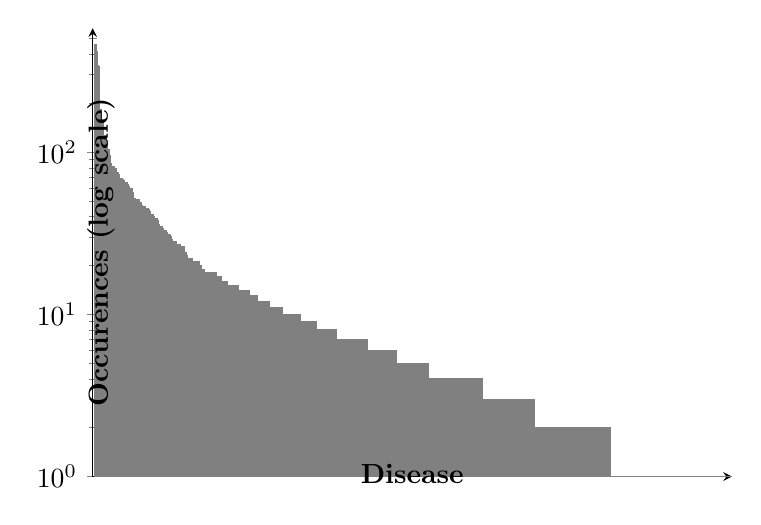
\begin{tikzpicture}
\begin{axis}[
    ybar,
    xmin=-2,
    ymin=-10,
    ymax=580,
    ymode=log, % Using logarithmic scale for y-axis
    log basis y=10,
    bar width=0.5pt,
    axis lines=left,
    width=0.8\textwidth,  % Scale to full text width
    height=0.6\textwidth, % Optional, for aspect ratio
    xlabel= {Disease},
    ylabel= {Occurences (log scale)},
    ylabel shift=-35pt, % Moves the y-label closer to the axis
    xlabel shift=-10pt, % Moves the x-label closer to the axis
    label style={font=\bfseries, fill=none},
    xtick=\empty,
    xticklabels=\empty,
    yticklabel style={fill=none}
    ]
\addplot+[
    fill=gray,
    draw=gray,
] coordinates {
    (0, 463)
 (1, 419)
 (2, 342)
 (3, 337)
 (4, 183)
 (5, 158)
 (6, 156)
 (7, 127)
 (8, 125)
 (9, 117)
 (10, 104)
 (11, 95)
 (12, 85)
 (13, 82)
 (14, 81)
 (15, 79)
 (16, 79)
 (17, 75)
 (18, 73)
 (19, 69)
 (20, 69)
 (21, 68)
 (22, 67)
 (23, 65)
 (24, 65)
 (25, 63)
 (26, 61)
 (27, 60)
 (28, 60)
 (29, 56)
 (30, 52)
 (31, 51)
 (32, 51)
 (33, 51)
 (34, 49)
 (35, 49)
 (36, 47)
 (37, 46)
 (38, 46)
 (39, 45)
 (40, 45)
 (41, 44)
 (42, 43)
 (43, 41)
 (44, 41)
 (45, 40)
 (46, 39)
 (47, 39)
 (48, 38)
 (49, 36)
 (50, 35)
 (51, 35)
 (52, 34)
 (53, 33)
 (54, 33)
 (55, 32)
 (56, 31)
 (57, 31)
 (58, 30)
 (59, 29)
 (60, 28)
 (61, 28)
 (62, 28)
 (63, 27)
 (64, 27)
 (65, 27)
 (66, 26)
 (67, 26)
 (68, 26)
 (69, 24)
 (70, 23)
 (71, 22)
 (72, 22)
 (73, 22)
 (74, 22)
 (75, 21)
 (76, 21)
 (77, 21)
 (78, 21)
 (79, 21)
 (80, 20)
 (81, 20)
 (82, 19)
 (83, 19)
 (84, 18)
 (85, 18)
 (86, 18)
 (87, 18)
 (88, 18)
 (89, 18)
 (90, 18)
 (91, 18)
 (92, 18)
 (93, 17)
 (94, 17)
 (95, 17)
 (96, 17)
 (97, 16)
 (98, 16)
 (99, 16)
 (100, 16)
 (101, 16)
 (102, 15)
 (103, 15)
 (104, 15)
 (105, 15)
 (106, 15)
 (107, 15)
 (108, 15)
 (109, 15)
 (110, 14)
 (111, 14)
 (112, 14)
 (113, 14)
 (114, 14)
 (115, 14)
 (116, 14)
 (117, 14)
 (118, 14)
 (119, 13)
 (120, 13)
 (121, 13)
 (122, 13)
 (123, 13)
 (124, 13)
 (125, 12)
 (126, 12)
 (127, 12)
 (128, 12)
 (129, 12)
 (130, 12)
 (131, 12)
 (132, 12)
 (133, 12)
 (134, 11)
 (135, 11)
 (136, 11)
 (137, 11)
 (138, 11)
 (139, 11)
 (140, 11)
 (141, 11)
 (142, 11)
 (143, 11)
 (144, 10)
 (145, 10)
 (146, 10)
 (147, 10)
 (148, 10)
 (149, 10)
 (150, 10)
 (151, 10)
 (152, 10)
 (153, 10)
 (154, 10)
 (155, 10)
 (156, 10)
 (157, 10)
 (158, 9)
 (159, 9)
 (160, 9)
 (161, 9)
 (162, 9)
 (163, 9)
 (164, 9)
 (165, 9)
 (166, 9)
 (167, 9)
 (168, 9)
 (169, 9)
 (170, 8)
 (171, 8)
 (172, 8)
 (173, 8)
 (174, 8)
 (175, 8)
 (176, 8)
 (177, 8)
 (178, 8)
 (179, 8)
 (180, 8)
 (181, 8)
 (182, 8)
 (183, 8)
 (184, 8)
 (185, 7)
 (186, 7)
 (187, 7)
 (188, 7)
 (189, 7)
 (190, 7)
 (191, 7)
 (192, 7)
 (193, 7)
 (194, 7)
 (195, 7)
 (196, 7)
 (197, 7)
 (198, 7)
 (199, 7)
 (200, 7)
 (201, 7)
 (202, 7)
 (203, 7)
 (204, 7)
 (205, 7)
 (206, 7)
 (207, 7)
 (208, 7)
 (209, 6)
 (210, 6)
 (211, 6)
 (212, 6)
 (213, 6)
 (214, 6)
 (215, 6)
 (216, 6)
 (217, 6)
 (218, 6)
 (219, 6)
 (220, 6)
 (221, 6)
 (222, 6)
 (223, 6)
 (224, 6)
 (225, 6)
 (226, 6)
 (227, 6)
 (228, 6)
 (229, 6)
 (230, 6)
 (231, 5)
 (232, 5)
 (233, 5)
 (234, 5)
 (235, 5)
 (236, 5)
 (237, 5)
 (238, 5)
 (239, 5)
 (240, 5)
 (241, 5)
 (242, 5)
 (243, 5)
 (244, 5)
 (245, 5)
 (246, 5)
 (247, 5)
 (248, 5)
 (249, 5)
 (250, 5)
 (251, 5)
 (252, 5)
 (253, 5)
 (254, 5)
 (255, 5)
 (256, 4)
 (257, 4)
 (258, 4)
 (259, 4)
 (260, 4)
 (261, 4)
 (262, 4)
 (263, 4)
 (264, 4)
 (265, 4)
 (266, 4)
 (267, 4)
 (268, 4)
 (269, 4)
 (270, 4)
 (271, 4)
 (272, 4)
 (273, 4)
 (274, 4)
 (275, 4)
 (276, 4)
 (277, 4)
 (278, 4)
 (279, 4)
 (280, 4)
 (281, 4)
 (282, 4)
 (283, 4)
 (284, 4)
 (285, 4)
 (286, 4)
 (287, 4)
 (288, 4)
 (289, 4)
 (290, 4)
 (291, 4)
 (292, 4)
 (293, 4)
 (294, 4)
 (295, 4)
 (296, 4)
 (297, 3)
 (298, 3)
 (299, 3)
 (300, 3)
 (301, 3)
 (302, 3)
 (303, 3)
 (304, 3)
 (305, 3)
 (306, 3)
 (307, 3)
 (308, 3)
 (309, 3)
 (310, 3)
 (311, 3)
 (312, 3)
 (313, 3)
 (314, 3)
 (315, 3)
 (316, 3)
 (317, 3)
 (318, 3)
 (319, 3)
 (320, 3)
 (321, 3)
 (322, 3)
 (323, 3)
 (324, 3)
 (325, 3)
 (326, 3)
 (327, 3)
 (328, 3)
 (329, 3)
 (330, 3)
 (331, 3)
 (332, 3)
 (333, 3)
 (334, 3)
 (335, 3)
 (336, 3)
 (337, 2)
 (338, 2)
 (339, 2)
 (340, 2)
 (341, 2)
 (342, 2)
 (343, 2)
 (344, 2)
 (345, 2)
 (346, 2)
 (347, 2)
 (348, 2)
 (349, 2)
 (350, 2)
 (351, 2)
 (352, 2)
 (353, 2)
 (354, 2)
 (355, 2)
 (356, 2)
 (357, 2)
 (358, 2)
 (359, 2)
 (360, 2)
 (361, 2)
 (362, 2)
 (363, 2)
 (364, 2)
 (365, 2)
 (366, 2)
 (367, 2)
 (368, 2)
 (369, 2)
 (370, 2)
 (371, 2)
 (372, 2)
 (373, 2)
 (374, 2)
 (375, 2)
 (376, 2)
 (377, 2)
 (378, 2)
 (379, 2)
 (380, 2)
 (381, 2)
 (382, 2)
 (383, 2)
 (384, 2)
 (385, 2)
 (386, 2)
 (387, 2)
 (388, 2)
 (389, 2)
 (390, 2)
 (391, 2)
 (392, 2)
 (393, 2)
 (394, 2)
 (395, 1)
 (396, 1)
 (397, 1)
 (398, 1)
 (399, 1)
 (400, 1)
 (401, 1)
 (402, 1)
 (403, 1)
 (404, 1)
 (405, 1)
 (406, 1)
 (407, 1)
 (408, 1)
 (409, 1)
 (410, 1)
 (411, 1)
 (412, 1)
 (413, 1)
 (414, 1)
 (415, 1)
 (416, 1)
 (417, 1)
 (418, 1)
 (419, 1)
 (420, 1)
 (421, 1)
 (422, 1)
 (423, 1)
 (424, 1)
 (425, 1)
 (426, 1)
 (427, 1)
 (428, 1)
 (429, 1)
 (430, 1)
 (431, 1)
 (432, 1)
 (433, 1)
 (434, 1)
 (435, 1)
 (436, 1)
 (437, 1)
 (438, 1)
 (439, 1)
 (440, 1)
 (441, 1)
 (442, 1)
 (443, 1)
 (444, 1)
 (445, 1)
 (446, 1)
 (447, 1)
 (448, 1)
 (449, 1)
 (450, 1)
 (451, 1)
 (452, 1)
 (453, 1)
 (454, 1)
 (455, 1)
 (456, 1)
 (457, 1)
 (458, 1)
 (459, 1)
 (460, 1)
 (461, 1)
 (462, 1)
 (463, 1)
 (464, 1)
 (465, 1)
 (466, 1)
 (467, 1)
 (468, 1)
 (469, 1)
 (470, 1)
 (471, 1)
 (472, 1)
 (473, 1)
 (474, 1)
 (475, 1)
 (476, 1)
 (477, 1)
 (478, 1)
 (479, 1)
 (480, 1)
 (481, 1)
 (482, 1)
 (483, 1)
 (484, 1)
 (485, 1)
 (486, 1)
 (487, 1)
 (488, 1)



};
\end{axis}
\end{tikzpicture}
\end{adjustbox}
\caption{Bar plot of Mendelian disease occurrence distribution in the Phenopacket Store.}
\label{fig:disease-histogram}
\end{figure}


\subsection{Data integration}
The patient data has been integrated with the underlying knowledge graph by adding nodes of type \emph{Person} and \emph{Article}. Specifically, the \emph{Person} nodes encompass the actual patients, alongside two nodes representing male and female sexes, respectively. For standardization purposes, the \emph{Male} and \emph{Female} nodes are identified using the following IRIs: \texttt{$\langle$http://purl.obolibrary.org/obo/NCIT\_C16576$\rangle$} and \texttt{$\langle$http://purl.obolibrary.org/obo/NCIT\_C20197$\rangle$}. Each article is refered to by \\ \texttt{$\langle$https://pubmed.ncbi.nlm.nih.gov/{article\_id}$\rangle$}. The nodes pertaining to patients extend the \emph{Article} identifiers by appending the patient code, resulting in a string of the form \\ \texttt{$\langle$https://pubmed.ncbi.nlm.nih.gov/{article\_id}?{patient\_code}$\rangle$}. 

We clarify the integration of the Phenopacket data with the underlying knowledge graph in \Cref{fig:patient_kg_hypergraph}, which specifies how the additional nodes have been interconnected with one another and with the existing \emph{Phenotype} and \emph{Disease} nodes. Henceforth, we will refer to the integrated knowledge graph as \emph{PatientKG}.
\begin{figure}
    \centering
    \begin{tikzpicture}
        % Nodes
        \node[circle, draw, fill=none, minimum size=2cm, inner sep=0pt] (Disease) at (1,4) {Disease};
        \node[circle, draw, fill=none, minimum size=2cm, inner sep=0pt] (Phenotype) at (-4,3) {Phenotype};
        \node[circle, draw, fill=none, minimum size=2cm, inner sep=0pt] (Article) at (2,9) {Article};
        \node[circle, draw, fill=none, minimum size=5cm, inner sep=0pt] (Person) at (-4,9) {Person};
        \node[circle, draw, dashed,  fill=none, minimum size=1.5cm, inner sep=0pt] (Male) at (-5,10.3) {\textit{Male}};
        \node[circle, draw, dashed, fill=none, minimum size=1.5cm, inner sep=0pt] (Female) at (-3,10.3) {\textit{Female}};
        \node[circle, draw, dashed, fill=none, minimum size=1.5cm, inner sep=0pt] (Patient) at (-4,7.4) {Patient};

        % Edges with curved labels
            \draw[->] (Person) to[bend right=10] (Article);
            \path[decorate, decoration={text along path, text align=center, raise=2pt, text={Part of}}] (Person) to[bend right=10] (Article);

            \draw[->] (Article) to[bend right=10] (Person);
            \path[decorate, decoration={text along path, text align=center, raise=2pt, text={Has part}}] (Person) to[bend left=10] (Article);

            \draw[dashed, ->] (Patient) to[bend left=30] (Male);
            \path[decorate, decoration={text along path, text align=center, raise=2pt, text={Subclassof}}] (Patient) to[bend left=30] (Male);
            \draw[dashed, ->] (Patient) to[bend right=30] (Female);
            \path[decorate, decoration={text along path, text align=center, raise=-8pt, text={Subclassof}}] (Patient) to[bend right=30] (Female);

            \draw[->] (Person) to[bend left=10] (Disease);
            \path[decorate, decoration={text along path, text align=center, raise=2pt, text={Has disease}}] (Person) to[bend left=10] (Disease);

            \draw[->] (Person) to[bend right=15] (Phenotype);
            \path[decorate, decoration={text along path, text align=center, raise=2pt, text={Has phenotype}}] (Phenotype) to[bend left=15] (Person);
            \draw[->] (Phenotype) to[bend right=10] (Person);
            \path[decorate, decoration={text along path, text align=center, raise=2pt, text={Phenotype of}}] (Phenotype) to[bend right=10] (Person);
    \end{tikzpicture}

    \caption{The hypergraph representing the node types and edge predicates added during the integration of the underlying knowledge graph and patient data. The nodes contained in the Person hypernode and the relative hyperedges are merely a semantic schematization of the data. In particular Male and Female correspond to single nodes in the knowledge graph.}
    \label{fig:patient_kg_hypergraph}
\end{figure}

\section{Link prediction for differential diagnosis}\label{sec:linkPredictionDiffDiagnosis}
In this section, we describe how we have employed PatientKG to address the challenge of differential diagnosis. We first adapt the problem to the PatientKG at our disposal.

\subsection{Experimental setup}
Utilizing PatientKG, the problem of differential diagnosis is reframed as the link prediction task involving edges of type \emph{Has disease} connecting the \emph{Person} nodes representing patients to the corresponding \emph{Disease} node. Considering the techniques evaluated in \Cref{grl}, we have chosen an inductive approach, specifically Graph Neural Networks (GNNs), to enable the model to generalize to previously unseen patients. In particular, we have selected the HGCN model, according to the reasoning discussed in \Cref{sec:hypPatientKG}.

To train the model for link prediction and evaluate its performance, the edges in PatientKG were partitioned into two sets: a test set composed of randomly selected \emph{Has disease} edges and a training set comprising the remaining \emph{Has disease} edges and all other edges in PatientKG. To regulate the learning process through early stopping, we also have extracted a validation set.

The distribution of cohorts by disease, illustrated in \Cref{fig:disease-histogram}, indicates that approximately half of the diseases represented in the Phenopacket Store have fewer than 10 cohorts, and roughly one-third have at most 5 occurrences. Given the limited availability of annotated disease diagnoses we have including in the test set only diseases with at least 5 cohorts. In addition we opted not to include \emph{Has disease} edges within the validation set utilized to monitor the learning process.

Since the test edges are derived from the relations provided by the Phenopacket Store, the model trained on the training set was evaluated on differential diagnoses exclusively among Mendelian diseases. This approach is logical as Mendelian diseases are often explored after all alternative common diagnoses have been ruled out. Preliminary experiments conducted using this data split revealed indications of potential overfitting. Since the articles typically pertain to specific diseases, the edges connecting patients to their corresponding articles of origin create a shortcut for inferring the patients' diseases. To prevent data leakage, we excluded all \emph{Has part} and \emph{Part of} edges linking the \emph{Person} nodes to the \emph{Article} nodes.

\medskip

In \cref{tab:hyperparams} we list how the main hyperparameters have been set across all experiments. The first three are related to the HGCN model, :
\begin{itemize}
  \item the number of layers $L$
  \item the number of attention heads $R$
  \item the activation function $\sigma$ 
\end{itemize}



% negative sampling

\subsection{Why hyperbolic graph representation learning?}\label{sec:hypPatientKG}
Prior to delving into the run experiments, we would like to account for the selection of hyperbolic graph representation learning techniques, specifically HGCN. As discussed in \Cref{sec:hyperbolicAndTrees}, hyperbolic geometry is particularly suited to represent hierarchical structures, such as those nested within PatientKG (refer to \Cref{sec:abstractGraphStructure}). To empirically verify this, we embedded each hierarchical component into hyperbolic space. To emphasize the positioning of each node within the hierarchy, we have considered the transitive closure of each subtree. The transitive closure of a directed graph is derived by adding an edge between every pair of nodes that are connected by a directed path. For instance, \Cref{fig:diseasePoincare} depicts the embedded \emph{Disease} nodes arranged within a Poincaré ball. One notices that nodes with a more extensive neighbourhood, i.e. nodes situated higher in the ontological hierarchy, are positioned closer to the centre of the ball. This representation can be interpreted as a real-world instance of the structure schematized in \Cref{fig:radialTree}, in accordance with the considerations articulated in \Cref{sec:expGrowth}. 
\begin{figure}
    \centering
    \begin{subfigure}[b]{0.6\textwidth}
        \centering
        \includegraphics[width=\textwidth]{figs/figDiseasePoincare.png}
    \end{subfigure}
    \begin{subfigure}[b]{0.1\textwidth}
        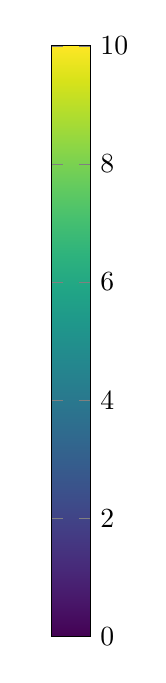
\begin{tikzpicture}
            \begin{axis}[
                hide axis,
                scale only axis,
                height=7.5cm,
                colorbar,
                colormap name=viridis,
                point meta min=0,
                point meta max=10,
                colorbar style={
                    height=7.5cm,
                    width=0.5cm,
                    ytick={0,2,...,10},
                    ticklabel style={fill=none, draw=none},
                    }      
                ]
                \addplot [draw=none, fill=none] coordinates {(0,0)};
            \end{axis}
        \end{tikzpicture}
    \end{subfigure}
    \label{fig:diseasePoincare}
    \caption{Shallow hyperbolic embeddings in the Poincaré disk of the \emph{Disease} hierarchical component. The color scale refers to the size of the neighbourhood of each node, in logarithmic scale.}

\end{figure}

Although the shallow embedding has yielded favorable results, we opted for an inductive graph representation technique, as touched on in the previous section. To ensure that the HGCN model would capture the hierarchical components within PatientKG, we assessed the model's performance exclusively on these subgraphs. In comparison, we conducted the same experiments using two representatives of advanced Euclidean GNN models, namely GCN (\Cref{sec:GCN}) and GAT (\Cref{sec:neighbourhoodAttention}). The hyperparameters employed in our experiments are detailed in Table~\ref{tab:hyperparams}; the number of attention heads is overlooked by the GCN model. For HGCN learning, the parameters for the Fermi-Dirac decoder are set to \texttt{r}=2 and \texttt{t}=1 (refer to \Cref{sec:linkPredictionHGCN}). These values were established based on hyperparameters recommended in the code repository provided by Hazy Research, which encompasses implementations of HGCN and other Euclidean and hyperbolic GNN models\footnote{We have utilized the implementations offered by the Hazy Research group at \url{https://github.com/HazyResearch/hgcn}. In particular, we have relied on their code for the shallow Poincaré ball embeddings, GCN, GAT models, and, of course, HGCN.}. 
\begin{table}
    \centering
    \caption{Hyperparameters used for training GCN, GAT and HGCN.}
    \label{tab:hyperparams}
    \begin{tabular}{rl}
        \toprule
        \textbf{Hyperparameter} & \textbf{Value} \\
        \midrule
        \texttt{Number of layers} & 2 \\
        \texttt{Number of heads} &  4 \\
        \texttt{Activation function} & ReLU \\
        \texttt{Weight decay} & 0.001 \\
        \texttt{Learning rate} & 0.001 \\
        \texttt{LR reduce frequency} & 5000 \\
        \texttt{Dropout} & 0.1 \\
        \texttt{Optimizer} & Adam \\
        \texttt{Momentum} & 0.999 \\
        \texttt{Gamma} & 0.5 \\        
        \texttt{Early stopping patience} & 100 \\
        \bottomrule
    \end{tabular}
\end{table}


In \Cref{tab:tabSubclassofPerf}, we display the performance of the three models resulting from a random split of the edges into training, validation, and test sets, with validation and test sets containing 10\% of the edges each. For evaluation for each edge we have produced a negative sample. We conducted a series of experiments while varying the desired embedding size. The evaluation of the predictions is expressed the cross-entropy loss for negative sampling\Cref{sec:crossEntropyLossNegSampling}, as well as the ROC\_AUC and average precision scores. As anticipated, performance improves upon increasing length of the hidden representation of the nodes. The results distinctly illustrate that HGCN surpasses Euclidean GNN models. The sole exception is observed within the \emph{Genomic feature} hierarchical component, where GCN and GAT yield slightly superior performance compared to HGCN at larger embedding sizes. In such instances, the loss remains elevated, suggesting that the models may be making incorrect predictions confidently. These tests confirm our confidence in employing HGCN for the link prediction task within PatientKG.
\begin{table} 
    \centering
    \caption{Performance of models HCGN, GAT and GCN on hierarchical components in PatientKG across different node types}
    \label{tab:tabSubclassofPerf}  
    \begin{subtable}[t]{\textwidth}
        \centering
        \begin{tabular}{r|ccc|ccc|ccc}        
            \toprule
            \multirow{2}{*}{\textbf{size}} & \multicolumn{3}{c|}{\textit{Loss}} & \multicolumn{3}{c|}{\textit{ROC\_AUC}} & \multicolumn{3}{c}{\textit{AP score}} \\
            & \textbf{GCN} & \textbf{GAT} & \textbf{HGCN} & \textbf{GCN} & \textbf{GAT} & \textbf{HGCN} & \textbf{GCN} & \textbf{GAT} & \textbf{HGCN} \\
            \midrule
                4 & 2.2522 & 2.2536 & \underline{1.2305} & 0.6289 & 0.5488 & \underline{0.9118} & 0.5913 & 0.5102 & \underline{0.9106} \\  
                8 & 2.2538 & 2.2523 & \underline{0.9730} & 0.6764 & 0.5836 & \underline{0.9442} & 0.6440 & 0.5744 & \underline{0.9584} \\
                16 & 2.2538 & 2.2532 & \underline{0.8388} & 0.7117 & 0.5963 & \underline{0.9479} & 0.7067 & 0.6977 & \underline{0.9615} \\
                32 & 2.2538 & 2.2532 & \underline{0.8666} & 0.7646 & 0.6984 & \underline{0.9527} & 0.7444 & 0.7077 & \underline{0.9647} \\
                64 & 2.2538 & 2.2514 & \underline{0.8539} & 0.7901 & 0.7020 & \underline{0.9484} & 0.7612 & 0.7430 & \underline{0.9637} \\
                100 & 2.2537 & 2.2451 & \underline{0.6406} & 0.8012 & 0.7107 & \underline{0.9573} & 0.7973 & 0.7415 & \underline{0.9604} \\
            \bottomrule
        \end{tabular}
        \caption{Node type \textit{Disease}}
    \end{subtable}
    
    \vspace{1em}
    
    \begin{subtable}[t]{\textwidth}
        \centering
        \begin{tabular}{r|ccc|ccc|ccc}      
            \toprule
            \multirow{2}{*}{\textbf{size}} & \multicolumn{3}{c|}{\textit{Loss}} & \multicolumn{3}{c|}{\textit{ROC\_AUC}} & \multicolumn{3}{c}{\textit{AP score}} \\
            & \textbf{GCN} & \textbf{GAT} & \textbf{HGCN} & \textbf{GCN} & \textbf{GAT} & \textbf{HGCN} & \textbf{GCN} & \textbf{GAT} & \textbf{HGCN} \\
            \midrule
            4 & 2.2539 & 2.2532 & \underline{2.3959} & \underline{0.7094} & 0.5958 & 0.7459 & \underline{0.6371} & 0.5268 & 0.6906 \\
            8 & 2.2538 & 2.2521 & \underline{1.3602} & 0.7353 & 0.5918 & \underline{0.8838} & 0.6796 & 0.5350 & \underline{0.8751} \\
            16 & 2.2538 & 2.2517 & \underline{1.0282} & 0.7770 & 0.6673 & \underline{0.9193} & 0.7415 & 0.6436 & \underline{0.9119} \\
            32 & 2.2538 & 2.2507 & \underline{1.0209} & 0.8628 & 0.7112 & \underline{0.9317} & 0.8249 & 0.7301 & \underline{0.9307} \\
            64 & 2.2533 & 2.2492 & \underline{1.3956} & \underline{0.9333} & 0.7374 & 0.8922 & \underline{0.9256} & 0.7765 & 0.9109 \\
            100 & 2.2538 & 2.2433 & \underline{1.0364} & \underline{0.9683} & 0.7604 & 0.9232 & \underline{0.9539} & 0.8028 & 0.9159 \\
            \bottomrule
        \end{tabular}
        \caption{Node type \textit{Genomic feature}}
    \end{subtable}
    
    \vspace{1em}
    
    \begin{subtable}[t]{\textwidth}
        \centering
        \begin{tabular}{r|ccc|ccc|ccc}   
             \toprule
                \multirow{2}{*}{\textbf{size}} & \multicolumn{3}{c|}{\textit{Loss}} & \multicolumn{3}{c|}{\textit{ROC\_AUC}} & \multicolumn{3}{c}{\textit{AP score}} \\
                & \textbf{GCN} & \textbf{GAT} & \textbf{HGCN} & \textbf{GCN} & \textbf{GAT} & \textbf{HGCN} & \textbf{GCN} & \textbf{GAT} & \textbf{HGCN} \\
                \midrule
                4 & 2.2538 & 2.2538 & \underline{0.8984} & 0.6441 & 0.6087 & \underline{0.7923} & 0.6152 & 0.5869 & \underline{0.8179} \\
                8 & 2.2538 & 2.2537 & \underline{0.7069} & 0.6627 & 0.6207 & \underline{0.8354} & 0.6513 & 0.6160 & \underline{0.8791} \\
                16 & 2.2538 & 2.2532 & \underline{0.6602} & 0.6992 & 0.6697 & \underline{0.8609} & 0.7059 & 0.6861 & \underline{0.8883} \\
                32 & 2.2538 & 2.2521 & \underline{0.6035} & 0.7403 & 0.6832 & \underline{0.8773} & 0.7265 & 0.7106 & \underline{0.9001} \\
                64 & 2.2535 & 2.2517 & \underline{0.5554} & 0.7569 & 0.7123 & \underline{0.9479} & 0.7598 & 0.7392 & \underline{0.9153} \\
                100 & 2.2534 & 2.2492 & \underline{0.5618} & 0.7742 & 0.7044 & \underline{0.9692} & 0.7749 & 0.7373 & \underline{0.9140} \\
                \bottomrule
        \end{tabular}
        \caption{Node type \textit{GO}}
    \end{subtable}
    
    \vspace{1em}
    
    \begin{subtable}[t]{\textwidth}
        \centering
        \begin{tabular}{r|ccc|ccc|ccc}   
        \toprule
            \multirow{2}{*}{\textbf{size}} & \multicolumn{3}{c|}{\textit{Loss}} & \multicolumn{3}{c|}{\textit{ROC\_AUC}} & \multicolumn{3}{c}{\textit{AP score}} \\
                & \textbf{GCN} & \textbf{GAT} & \textbf{HGCN} & \textbf{GCN} & \textbf{GAT} & \textbf{HGCN} & \textbf{GCN} & \textbf{GAT} & \textbf{HGCN} \\
            \midrule
            4 & 2.2539 & 2.2537 & \underline{1.4855} & 0.6289 & 0.6223 & \underline{0.9240} & 0.5947 & 0.6195 & \underline{0.9460} \\
            8 & 2.2538 & 2.2537 & \underline{1.3125} & 0.6501 & 0.6512 & \underline{0.9334} & 0.6284 & 0.6626 & \underline{0.9572} \\
            16 & 2.2538 & 2.2533 & \underline{1.1390} & 0.6848 & 0.6645 & \underline{0.9359} & 0.6728 & 0.7039 & \underline{0.9594} \\
            32 & 2.2538 & 2.2529 & \underline{0.9025} & 0.7036 & 0.6773 & \underline{0.9382} & 0.7017 & 0.7409 & \underline{0.9610} \\
            64 & 2.2538 & 2.2510 & \underline{0.6700} & 0.7276 & 0.6842 & \underline{0.9452} & 0.7119 & 0.7617 & \underline{0.9633} \\
            100 & 2.2538 & 2.2389 & \underline{0.6079} & 0.7567 & 0.6555 & \underline{0.9573} & 0.7318 & 0.7713 & \underline{0.9688} \\
            \bottomrule
        \end{tabular}
        \caption{Node type \textit{Phenotype}}
    \end{subtable}
\end{table}


We are aware of more advanced techniques than HGCN that are tailored to knowledge graph applications. In particular, we highlight the \textsc{Att\_H} model~\cite{chami2020lowDimensionalHyperbolicKnowledgeGraphEmbeddings}, proposed by the authors of HGCN. Their rationale is that existing hyperbolic embedding methods do not adequately account for the logical patterns present in knowledge graphs, which we have referred to as "horizontal" links. Consequently, they introduce a class of hyperbolic KG embedding models that simultaneously capture hierarchical and logical patterns by combining hyperbolic reflections and rotations with attention. We have chosen to stick with a model like HGCN that emphasizes the hierarchical components, as we were interested in evaluating whether this approach would be sufficient to address the challenges of differential diagnosis. We leave the exploration of more advanced hyperbolic models for future work.

\subsection{Managing a large graph}
As seen in the description of the HGCN architecture, the aggregation step (\Cref{sec:hgcnAggregation}) requires the model to access the neighbourhoods of each node. In the code implemented in the Hazy Research repository this information is provided in the form of an adjacency matrix of the whole input graph. However for large graphs like PatientKG, this approach is not feasible due to memory constraints, especially considering that the model is trained and evaluated on GPU.
Seen these limitations it was necessary to settle for the more general global version of the aggregation step. 
To further overcome this issue we have initially attempted to reimplement the model using sparse matrices, keeping in mind the properties of PatientKG's adjacency matrix. Unfortunately we encountered various technical issues since the \texttt{PyTorch} library used to implement HGCN is ill equipped to handle sparse tensors. The attempted solution entailed specifying methods, among others, for sparse-sparse and sparse-dense matrix division, row-wise normalization, and various hyperbolic functions, such as the hyperbolic tangent. However, accounting for forward and backward passes, we were unable to achieve a working implementation considering the time constraints and scope of this thesis.

We then opted for a more straightforward solution, that is to use mini-batching of the graph. We now discuss the validity of this choice and how we have implemented this approach in our experiments.

\subsubsection{Mini-batching}

Training deep neural networks (DNNs) typically involves processing independent and identically distributed (i.i.d.) examples, whereas graph neural networks (GNNs) operate on interconnected vertices within a graph structure, introducing dependencies that complicate training. GNNs can be trained using either full-graph (full-batch) or mini-batch approaches~\cite{bajaj2024graph}.

In full-graph training, message-passing is performed across the entire graph in each epoch, ensuring that all vertex dependencies are considered. However, this method becomes computationally expensive and memory-intensive for large graphs, requiring multi-GPU model parallelism where the graph is partitioned and hidden features are exchanged across GPUs. While full-graph training avoids information loss by processing the complete graph, its high per-epoch cost and communication overhead make scaling difficult.

Mini-batch training, in contrast, splits the graph into smaller subgraphs (batches) and processes them iteratively, updating model parameters multiple times per epoch. However, preparing these mini-batches is non-trivial because GNNs require $k$-hop neighbourhood aggregation—meaning that for a GNN with $L$ layers, each batch must include vertices up to $L$ hops away to ensure correct message-passing. This leads to the neighbourhood explosion problem, where the required subgraph grows exponentially with depth, making full neighbourhood aggregation impractical. To mitigate this, mini-batch systems use sampling techniques (e.g., Neighbourhood Sampling, ClusterGCN, GraphSAINT) to load only a subset of the k-hop neighbours, trading off some accuracy for efficiency. 

Despite these challenges, mini-batch training often converges faster in practice because it performs multiple parameter updates per epoch, whereas full-graph training updates only once per epoch. Also the simple Neighbourhood Sampling method empirically shows a more stable behaviour.

To implement the batching of PatientKG into subgraphs we have relied on the \texttt{torch-geometric} library~\cite{fey2019pytorchGeometric}. More specifically we have chosen to sample the subgraphs using the \texttt{NeighborSampler} class. This class is designed to sample a fixed-size batch of so called seed nodes, and for each of these it samples their neighbourhood. For each seed node one can specify a list of integers $[n_1, n_2, \dots, n_k]$, such that $n_1$ of its neighbours are sampled, then from each of those 1-hop neighbours $n_2$ neighbours are sampled, and so on, until $n_k$ neighbours are sampled from the $k$-th hop neighbours. The sampling is performed in a breadth-first manner, meaning that all nodes at the first hop are sampled before moving to the second hop, and so on. This approach allows us to control the size and the of the subgraphs sampled, letting us determine the size of the input adjacency matrix a priori. This sampling strategy implies that all the nodes are seen at least once by the model when they are seed nodes of a given batch, and can be re-extracted if they are selected among the sampled neighbours of other nodes. 

Like when batching in classical machine learning settings, on each local sample the forward and backward passes are performed independently, and the weights of the model are updated after each batch. The weights are updated according to the loss value computed on only the seed nodes in each batch. Empirically, we have found that computing the loss over all batch nodes to guide backpropagation causes overfitting. Focusing on seed nodes prevents the backpropagation signal from being diluted across thousands of neighbours. This choice allows the model to learn more effectively from the most relevant nodes in each batch, while still benefiting from the rich information provided by their neighbors.


To assure the compatibility among batches it was necessary to set the curvature of the hyperbolic space to a fixed value, which we have set to $c=1$. This derives from the definition of the Poincaré ball model (\Cref{sec:poincareBall}).

\medskip 

In addition to the hyperparameters listed in \Cref{tab:hyperparams}, we also hae set the batch size and neighbourhood sample sizes. Using the parameters in GraphSAGE~\cite{Hamilton2017inductiveRepresentationLearning}, we set the neighbourhood sample sizes to $n_1=25$ and $n_2=10$ since we were working with a 2 layer model. To respect memory constraints we have set the batch size to $172$. In addition we have tested the model on batches formed by fewer extracted nodes, but with additional hops from the seed nodes. Concretely the list describing the neighbourhood sample sizes was set to $[5,3,3,3]$. In this case we were able to increase the batch size to $235$ nodes.

\subsubsection{Final inference step}
Recall from \Cref{sec:hgcnArchitecture} that the link prediction task requires the encoded embeddings to be decoded to compute the probability scores among the edges. Note that when encoding a subgraph the resulting embeddings refer only to that subset of nodes. This does not pose a problem during training seen that the embeddings local to the batch are sufficient to compute the local loss for the backward pass. In the case of validation and testing, however, one needs the embeddings of all the nodes to compute the link prediction scores. To address this, one adds a final inference step after training. This involves running a forward pass on (ideally) the entire graph. As discussed before, for PatientKG this is not feasible due to memory constraints, therefore one can load the full graph in manageable chunks, made up of some seed nodes and their whole neighbourhoods. In this way the forward pass is as similar as possible to the full-graph inference. 

In \Cref{fig:neighDistr} we plot the distribution of the neighbourhood sizes among nodes in PatientKG. The distribution is highly skewed, as put in evidence by the knee point in the plot\footnote{The knee point has been located using the kneedle algorithm~\cite{satopaa2011KneePointDetection}}. This has allowed us to reduce the memory footprint during inference by creating batches mad up of few large neighbourhood nodes and a lot of small neighbourhood nodes. 
\begin{figure}
    \centering
\begin{adjustbox}{margin=-2cm 0cm 0cm 0cm} % Left, Bottom, Right, Top margins

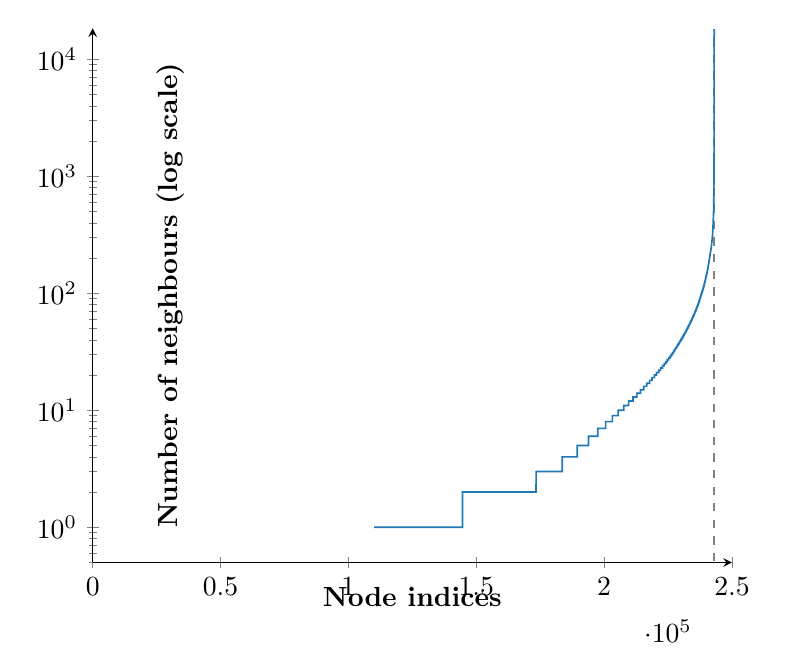
\begin{tikzpicture}
\definecolor{darkgray176}{RGB}{176,176,176}
\definecolor{steelblue31119180}{RGB}{31,119,180}

\begin{axis}[
    width=0.8\textwidth,
    tick align=outside,
    ymode=log,
    log basis y=10,
    xmin=0, xmax=250000,
    ymin=0.5, ymax=18425,
    axis lines=left,
    label style={font=\bfseries, fill=none},
    xticklabel style={fill=none},
    yticklabel style={fill=none},
    xlabel=Node indices,
    ylabel=Number of neighbours (log scale),
    xlabel shift=-10pt,
    ylabel shift=-60pt
]
\addplot [gray, dashed, thick] coordinates {(242898,0.1) (242898,18000)};
    
\addplot [semithick, steelblue31119180]
table {%
0 0
10 0
20 0
30 0
40 0
50 0
60 0
70 0
80 0
90 0
100 0
110 0
120 0
130 0
140 0
150 0
160 0
170 0
180 0
190 0
200 0
210 0
220 0
230 0
240 0
250 0
260 0
270 0
280 0
290 0
300 0
310 0
320 0
330 0
340 0
350 0
360 0
370 0
380 0
390 0
400 0
410 0
420 0
430 0
440 0
450 0
460 0
470 0
480 0
490 0
500 0
510 0
520 0
530 0
540 0
550 0
560 0
570 0
580 0
590 0
600 0
610 0
620 0
630 0
640 0
650 0
660 0
670 0
680 0
690 0
700 0
710 0
720 0
730 0
740 0
750 0
760 0
770 0
780 0
790 0
800 0
810 0
820 0
830 0
840 0
850 0
860 0
870 0
880 0
890 0
900 0
910 0
920 0
930 0
940 0
950 0
960 0
970 0
980 0
990 0
1000 0
1010 0
1020 0
1030 0
1040 0
1050 0
1060 0
1070 0
1080 0
1090 0
1100 0
1110 0
1120 0
1130 0
1140 0
1150 0
1160 0
1170 0
1180 0
1190 0
1200 0
1210 0
1220 0
1230 0
1240 0
1250 0
1260 0
1270 0
1280 0
1290 0
1300 0
1310 0
1320 0
1330 0
1340 0
1350 0
1360 0
1370 0
1380 0
1390 0
1400 0
1410 0
1420 0
1430 0
1440 0
1450 0
1460 0
1470 0
1480 0
1490 0
1500 0
1510 0
1520 0
1530 0
1540 0
1550 0
1560 0
1570 0
1580 0
1590 0
1600 0
1610 0
1620 0
1630 0
1640 0
1650 0
1660 0
1670 0
1680 0
1690 0
1700 0
1710 0
1720 0
1730 0
1740 0
1750 0
1760 0
1770 0
1780 0
1790 0
1800 0
1810 0
1820 0
1830 0
1840 0
1850 0
1860 0
1870 0
1880 0
1890 0
1900 0
1910 0
1920 0
1930 0
1940 0
1950 0
1960 0
1970 0
1980 0
1990 0
2000 0
2010 0
2020 0
2030 0
2040 0
2050 0
2060 0
2070 0
2080 0
2090 0
2100 0
2110 0
2120 0
2130 0
2140 0
2150 0
2160 0
2170 0
2180 0
2190 0
2200 0
2210 0
2220 0
2230 0
2240 0
2250 0
2260 0
2270 0
2280 0
2290 0
2300 0
2310 0
2320 0
2330 0
2340 0
2350 0
2360 0
2370 0
2380 0
2390 0
2400 0
2410 0
2420 0
2430 0
2440 0
2450 0
2460 0
2470 0
2480 0
2490 0
2500 0
2510 0
2520 0
2530 0
2540 0
2550 0
2560 0
2570 0
2580 0
2590 0
2600 0
2610 0
2620 0
2630 0
2640 0
2650 0
2660 0
2670 0
2680 0
2690 0
2700 0
2710 0
2720 0
2730 0
2740 0
2750 0
2760 0
2770 0
2780 0
2790 0
2800 0
2810 0
2820 0
2830 0
2840 0
2850 0
2860 0
2870 0
2880 0
2890 0
2900 0
2910 0
2920 0
2930 0
2940 0
2950 0
2960 0
2970 0
2980 0
2990 0
3000 0
3010 0
3020 0
3030 0
3040 0
3050 0
3060 0
3070 0
3080 0
3090 0
3100 0
3110 0
3120 0
3130 0
3140 0
3150 0
3160 0
3170 0
3180 0
3190 0
3200 0
3210 0
3220 0
3230 0
3240 0
3250 0
3260 0
3270 0
3280 0
3290 0
3300 0
3310 0
3320 0
3330 0
3340 0
3350 0
3360 0
3370 0
3380 0
3390 0
3400 0
3410 0
3420 0
3430 0
3440 0
3450 0
3460 0
3470 0
3480 0
3490 0
3500 0
3510 0
3520 0
3530 0
3540 0
3550 0
3560 0
3570 0
3580 0
3590 0
3600 0
3610 0
3620 0
3630 0
3640 0
3650 0
3660 0
3670 0
3680 0
3690 0
3700 0
3710 0
3720 0
3730 0
3740 0
3750 0
3760 0
3770 0
3780 0
3790 0
3800 0
3810 0
3820 0
3830 0
3840 0
3850 0
3860 0
3870 0
3880 0
3890 0
3900 0
3910 0
3920 0
3930 0
3940 0
3950 0
3960 0
3970 0
3980 0
3990 0
4000 0
4010 0
4020 0
4030 0
4040 0
4050 0
4060 0
4070 0
4080 0
4090 0
4100 0
4110 0
4120 0
4130 0
4140 0
4150 0
4160 0
4170 0
4180 0
4190 0
4200 0
4210 0
4220 0
4230 0
4240 0
4250 0
4260 0
4270 0
4280 0
4290 0
4300 0
4310 0
4320 0
4330 0
4340 0
4350 0
4360 0
4370 0
4380 0
4390 0
4400 0
4410 0
4420 0
4430 0
4440 0
4450 0
4460 0
4470 0
4480 0
4490 0
4500 0
4510 0
4520 0
4530 0
4540 0
4550 0
4560 0
4570 0
4580 0
4590 0
4600 0
4610 0
4620 0
4630 0
4640 0
4650 0
4660 0
4670 0
4680 0
4690 0
4700 0
4710 0
4720 0
4730 0
4740 0
4750 0
4760 0
4770 0
4780 0
4790 0
4800 0
4810 0
4820 0
4830 0
4840 0
4850 0
4860 0
4870 0
4880 0
4890 0
4900 0
4910 0
4920 0
4930 0
4940 0
4950 0
4960 0
4970 0
4980 0
4990 0
5000 0
5010 0
5020 0
5030 0
5040 0
5050 0
5060 0
5070 0
5080 0
5090 0
5100 0
5110 0
5120 0
5130 0
5140 0
5150 0
5160 0
5170 0
5180 0
5190 0
5200 0
5210 0
5220 0
5230 0
5240 0
5250 0
5260 0
5270 0
5280 0
5290 0
5300 0
5310 0
5320 0
5330 0
5340 0
5350 0
5360 0
5370 0
5380 0
5390 0
5400 0
5410 0
5420 0
5430 0
5440 0
5450 0
5460 0
5470 0
5480 0
5490 0
5500 0
5510 0
5520 0
5530 0
5540 0
5550 0
5560 0
5570 0
5580 0
5590 0
5600 0
5610 0
5620 0
5630 0
5640 0
5650 0
5660 0
5670 0
5680 0
5690 0
5700 0
5710 0
5720 0
5730 0
5740 0
5750 0
5760 0
5770 0
5780 0
5790 0
5800 0
5810 0
5820 0
5830 0
5840 0
5850 0
5860 0
5870 0
5880 0
5890 0
5900 0
5910 0
5920 0
5930 0
5940 0
5950 0
5960 0
5970 0
5980 0
5990 0
6000 0
6010 0
6020 0
6030 0
6040 0
6050 0
6060 0
6070 0
6080 0
6090 0
6100 0
6110 0
6120 0
6130 0
6140 0
6150 0
6160 0
6170 0
6180 0
6190 0
6200 0
6210 0
6220 0
6230 0
6240 0
6250 0
6260 0
6270 0
6280 0
6290 0
6300 0
6310 0
6320 0
6330 0
6340 0
6350 0
6360 0
6370 0
6380 0
6390 0
6400 0
6410 0
6420 0
6430 0
6440 0
6450 0
6460 0
6470 0
6480 0
6490 0
6500 0
6510 0
6520 0
6530 0
6540 0
6550 0
6560 0
6570 0
6580 0
6590 0
6600 0
6610 0
6620 0
6630 0
6640 0
6650 0
6660 0
6670 0
6680 0
6690 0
6700 0
6710 0
6720 0
6730 0
6740 0
6750 0
6760 0
6770 0
6780 0
6790 0
6800 0
6810 0
6820 0
6830 0
6840 0
6850 0
6860 0
6870 0
6880 0
6890 0
6900 0
6910 0
6920 0
6930 0
6940 0
6950 0
6960 0
6970 0
6980 0
6990 0
7000 0
7010 0
7020 0
7030 0
7040 0
7050 0
7060 0
7070 0
7080 0
7090 0
7100 0
7110 0
7120 0
7130 0
7140 0
7150 0
7160 0
7170 0
7180 0
7190 0
7200 0
7210 0
7220 0
7230 0
7240 0
7250 0
7260 0
7270 0
7280 0
7290 0
7300 0
7310 0
7320 0
7330 0
7340 0
7350 0
7360 0
7370 0
7380 0
7390 0
7400 0
7410 0
7420 0
7430 0
7440 0
7450 0
7460 0
7470 0
7480 0
7490 0
7500 0
7510 0
7520 0
7530 0
7540 0
7550 0
7560 0
7570 0
7580 0
7590 0
7600 0
7610 0
7620 0
7630 0
7640 0
7650 0
7660 0
7670 0
7680 0
7690 0
7700 0
7710 0
7720 0
7730 0
7740 0
7750 0
7760 0
7770 0
7780 0
7790 0
7800 0
7810 0
7820 0
7830 0
7840 0
7850 0
7860 0
7870 0
7880 0
7890 0
7900 0
7910 0
7920 0
7930 0
7940 0
7950 0
7960 0
7970 0
7980 0
7990 0
8000 0
8010 0
8020 0
8030 0
8040 0
8050 0
8060 0
8070 0
8080 0
8090 0
8100 0
8110 0
8120 0
8130 0
8140 0
8150 0
8160 0
8170 0
8180 0
8190 0
8200 0
8210 0
8220 0
8230 0
8240 0
8250 0
8260 0
8270 0
8280 0
8290 0
8300 0
8310 0
8320 0
8330 0
8340 0
8350 0
8360 0
8370 0
8380 0
8390 0
8400 0
8410 0
8420 0
8430 0
8440 0
8450 0
8460 0
8470 0
8480 0
8490 0
8500 0
8510 0
8520 0
8530 0
8540 0
8550 0
8560 0
8570 0
8580 0
8590 0
8600 0
8610 0
8620 0
8630 0
8640 0
8650 0
8660 0
8670 0
8680 0
8690 0
8700 0
8710 0
8720 0
8730 0
8740 0
8750 0
8760 0
8770 0
8780 0
8790 0
8800 0
8810 0
8820 0
8830 0
8840 0
8850 0
8860 0
8870 0
8880 0
8890 0
8900 0
8910 0
8920 0
8930 0
8940 0
8950 0
8960 0
8970 0
8980 0
8990 0
9000 0
9010 0
9020 0
9030 0
9040 0
9050 0
9060 0
9070 0
9080 0
9090 0
9100 0
9110 0
9120 0
9130 0
9140 0
9150 0
9160 0
9170 0
9180 0
9190 0
9200 0
9210 0
9220 0
9230 0
9240 0
9250 0
9260 0
9270 0
9280 0
9290 0
9300 0
9310 0
9320 0
9330 0
9340 0
9350 0
9360 0
9370 0
9380 0
9390 0
9400 0
9410 0
9420 0
9430 0
9440 0
9450 0
9460 0
9470 0
9480 0
9490 0
9500 0
9510 0
9520 0
9530 0
9540 0
9550 0
9560 0
9570 0
9580 0
9590 0
9600 0
9610 0
9620 0
9630 0
9640 0
9650 0
9660 0
9670 0
9680 0
9690 0
9700 0
9710 0
9720 0
9730 0
9740 0
9750 0
9760 0
9770 0
9780 0
9790 0
9800 0
9810 0
9820 0
9830 0
9840 0
9850 0
9860 0
9870 0
9880 0
9890 0
9900 0
9910 0
9920 0
9930 0
9940 0
9950 0
9960 0
9970 0
9980 0
9990 0
10000 0
10010 0
10020 0
10030 0
10040 0
10050 0
10060 0
10070 0
10080 0
10090 0
10100 0
10110 0
10120 0
10130 0
10140 0
10150 0
10160 0
10170 0
10180 0
10190 0
10200 0
10210 0
10220 0
10230 0
10240 0
10250 0
10260 0
10270 0
10280 0
10290 0
10300 0
10310 0
10320 0
10330 0
10340 0
10350 0
10360 0
10370 0
10380 0
10390 0
10400 0
10410 0
10420 0
10430 0
10440 0
10450 0
10460 0
10470 0
10480 0
10490 0
10500 0
10510 0
10520 0
10530 0
10540 0
10550 0
10560 0
10570 0
10580 0
10590 0
10600 0
10610 0
10620 0
10630 0
10640 0
10650 0
10660 0
10670 0
10680 0
10690 0
10700 0
10710 0
10720 0
10730 0
10740 0
10750 0
10760 0
10770 0
10780 0
10790 0
10800 0
10810 0
10820 0
10830 0
10840 0
10850 0
10860 0
10870 0
10880 0
10890 0
10900 0
10910 0
10920 0
10930 0
10940 0
10950 0
10960 0
10970 0
10980 0
10990 0
11000 0
11010 0
11020 0
11030 0
11040 0
11050 0
11060 0
11070 0
11080 0
11090 0
11100 0
11110 0
11120 0
11130 0
11140 0
11150 0
11160 0
11170 0
11180 0
11190 0
11200 0
11210 0
11220 0
11230 0
11240 0
11250 0
11260 0
11270 0
11280 0
11290 0
11300 0
11310 0
11320 0
11330 0
11340 0
11350 0
11360 0
11370 0
11380 0
11390 0
11400 0
11410 0
11420 0
11430 0
11440 0
11450 0
11460 0
11470 0
11480 0
11490 0
11500 0
11510 0
11520 0
11530 0
11540 0
11550 0
11560 0
11570 0
11580 0
11590 0
11600 0
11610 0
11620 0
11630 0
11640 0
11650 0
11660 0
11670 0
11680 0
11690 0
11700 0
11710 0
11720 0
11730 0
11740 0
11750 0
11760 0
11770 0
11780 0
11790 0
11800 0
11810 0
11820 0
11830 0
11840 0
11850 0
11860 0
11870 0
11880 0
11890 0
11900 0
11910 0
11920 0
11930 0
11940 0
11950 0
11960 0
11970 0
11980 0
11990 0
12000 0
12010 0
12020 0
12030 0
12040 0
12050 0
12060 0
12070 0
12080 0
12090 0
12100 0
12110 0
12120 0
12130 0
12140 0
12150 0
12160 0
12170 0
12180 0
12190 0
12200 0
12210 0
12220 0
12230 0
12240 0
12250 0
12260 0
12270 0
12280 0
12290 0
12300 0
12310 0
12320 0
12330 0
12340 0
12350 0
12360 0
12370 0
12380 0
12390 0
12400 0
12410 0
12420 0
12430 0
12440 0
12450 0
12460 0
12470 0
12480 0
12490 0
12500 0
12510 0
12520 0
12530 0
12540 0
12550 0
12560 0
12570 0
12580 0
12590 0
12600 0
12610 0
12620 0
12630 0
12640 0
12650 0
12660 0
12670 0
12680 0
12690 0
12700 0
12710 0
12720 0
12730 0
12740 0
12750 0
12760 0
12770 0
12780 0
12790 0
12800 0
12810 0
12820 0
12830 0
12840 0
12850 0
12860 0
12870 0
12880 0
12890 0
12900 0
12910 0
12920 0
12930 0
12940 0
12950 0
12960 0
12970 0
12980 0
12990 0
13000 0
13010 0
13020 0
13030 0
13040 0
13050 0
13060 0
13070 0
13080 0
13090 0
13100 0
13110 0
13120 0
13130 0
13140 0
13150 0
13160 0
13170 0
13180 0
13190 0
13200 0
13210 0
13220 0
13230 0
13240 0
13250 0
13260 0
13270 0
13280 0
13290 0
13300 0
13310 0
13320 0
13330 0
13340 0
13350 0
13360 0
13370 0
13380 0
13390 0
13400 0
13410 0
13420 0
13430 0
13440 0
13450 0
13460 0
13470 0
13480 0
13490 0
13500 0
13510 0
13520 0
13530 0
13540 0
13550 0
13560 0
13570 0
13580 0
13590 0
13600 0
13610 0
13620 0
13630 0
13640 0
13650 0
13660 0
13670 0
13680 0
13690 0
13700 0
13710 0
13720 0
13730 0
13740 0
13750 0
13760 0
13770 0
13780 0
13790 0
13800 0
13810 0
13820 0
13830 0
13840 0
13850 0
13860 0
13870 0
13880 0
13890 0
13900 0
13910 0
13920 0
13930 0
13940 0
13950 0
13960 0
13970 0
13980 0
13990 0
14000 0
14010 0
14020 0
14030 0
14040 0
14050 0
14060 0
14070 0
14080 0
14090 0
14100 0
14110 0
14120 0
14130 0
14140 0
14150 0
14160 0
14170 0
14180 0
14190 0
14200 0
14210 0
14220 0
14230 0
14240 0
14250 0
14260 0
14270 0
14280 0
14290 0
14300 0
14310 0
14320 0
14330 0
14340 0
14350 0
14360 0
14370 0
14380 0
14390 0
14400 0
14410 0
14420 0
14430 0
14440 0
14450 0
14460 0
14470 0
14480 0
14490 0
14500 0
14510 0
14520 0
14530 0
14540 0
14550 0
14560 0
14570 0
14580 0
14590 0
14600 0
14610 0
14620 0
14630 0
14640 0
14650 0
14660 0
14670 0
14680 0
14690 0
14700 0
14710 0
14720 0
14730 0
14740 0
14750 0
14760 0
14770 0
14780 0
14790 0
14800 0
14810 0
14820 0
14830 0
14840 0
14850 0
14860 0
14870 0
14880 0
14890 0
14900 0
14910 0
14920 0
14930 0
14940 0
14950 0
14960 0
14970 0
14980 0
14990 0
15000 0
15010 0
15020 0
15030 0
15040 0
15050 0
15060 0
15070 0
15080 0
15090 0
15100 0
15110 0
15120 0
15130 0
15140 0
15150 0
15160 0
15170 0
15180 0
15190 0
15200 0
15210 0
15220 0
15230 0
15240 0
15250 0
15260 0
15270 0
15280 0
15290 0
15300 0
15310 0
15320 0
15330 0
15340 0
15350 0
15360 0
15370 0
15380 0
15390 0
15400 0
15410 0
15420 0
15430 0
15440 0
15450 0
15460 0
15470 0
15480 0
15490 0
15500 0
15510 0
15520 0
15530 0
15540 0
15550 0
15560 0
15570 0
15580 0
15590 0
15600 0
15610 0
15620 0
15630 0
15640 0
15650 0
15660 0
15670 0
15680 0
15690 0
15700 0
15710 0
15720 0
15730 0
15740 0
15750 0
15760 0
15770 0
15780 0
15790 0
15800 0
15810 0
15820 0
15830 0
15840 0
15850 0
15860 0
15870 0
15880 0
15890 0
15900 0
15910 0
15920 0
15930 0
15940 0
15950 0
15960 0
15970 0
15980 0
15990 0
16000 0
16010 0
16020 0
16030 0
16040 0
16050 0
16060 0
16070 0
16080 0
16090 0
16100 0
16110 0
16120 0
16130 0
16140 0
16150 0
16160 0
16170 0
16180 0
16190 0
16200 0
16210 0
16220 0
16230 0
16240 0
16250 0
16260 0
16270 0
16280 0
16290 0
16300 0
16310 0
16320 0
16330 0
16340 0
16350 0
16360 0
16370 0
16380 0
16390 0
16400 0
16410 0
16420 0
16430 0
16440 0
16450 0
16460 0
16470 0
16480 0
16490 0
16500 0
16510 0
16520 0
16530 0
16540 0
16550 0
16560 0
16570 0
16580 0
16590 0
16600 0
16610 0
16620 0
16630 0
16640 0
16650 0
16660 0
16670 0
16680 0
16690 0
16700 0
16710 0
16720 0
16730 0
16740 0
16750 0
16760 0
16770 0
16780 0
16790 0
16800 0
16810 0
16820 0
16830 0
16840 0
16850 0
16860 0
16870 0
16880 0
16890 0
16900 0
16910 0
16920 0
16930 0
16940 0
16950 0
16960 0
16970 0
16980 0
16990 0
17000 0
17010 0
17020 0
17030 0
17040 0
17050 0
17060 0
17070 0
17080 0
17090 0
17100 0
17110 0
17120 0
17130 0
17140 0
17150 0
17160 0
17170 0
17180 0
17190 0
17200 0
17210 0
17220 0
17230 0
17240 0
17250 0
17260 0
17270 0
17280 0
17290 0
17300 0
17310 0
17320 0
17330 0
17340 0
17350 0
17360 0
17370 0
17380 0
17390 0
17400 0
17410 0
17420 0
17430 0
17440 0
17450 0
17460 0
17470 0
17480 0
17490 0
17500 0
17510 0
17520 0
17530 0
17540 0
17550 0
17560 0
17570 0
17580 0
17590 0
17600 0
17610 0
17620 0
17630 0
17640 0
17650 0
17660 0
17670 0
17680 0
17690 0
17700 0
17710 0
17720 0
17730 0
17740 0
17750 0
17760 0
17770 0
17780 0
17790 0
17800 0
17810 0
17820 0
17830 0
17840 0
17850 0
17860 0
17870 0
17880 0
17890 0
17900 0
17910 0
17920 0
17930 0
17940 0
17950 0
17960 0
17970 0
17980 0
17990 0
18000 0
18010 0
18020 0
18030 0
18040 0
18050 0
18060 0
18070 0
18080 0
18090 0
18100 0
18110 0
18120 0
18130 0
18140 0
18150 0
18160 0
18170 0
18180 0
18190 0
18200 0
18210 0
18220 0
18230 0
18240 0
18250 0
18260 0
18270 0
18280 0
18290 0
18300 0
18310 0
18320 0
18330 0
18340 0
18350 0
18360 0
18370 0
18380 0
18390 0
18400 0
18410 0
18420 0
18430 0
18440 0
18450 0
18460 0
18470 0
18480 0
18490 0
18500 0
18510 0
18520 0
18530 0
18540 0
18550 0
18560 0
18570 0
18580 0
18590 0
18600 0
18610 0
18620 0
18630 0
18640 0
18650 0
18660 0
18670 0
18680 0
18690 0
18700 0
18710 0
18720 0
18730 0
18740 0
18750 0
18760 0
18770 0
18780 0
18790 0
18800 0
18810 0
18820 0
18830 0
18840 0
18850 0
18860 0
18870 0
18880 0
18890 0
18900 0
18910 0
18920 0
18930 0
18940 0
18950 0
18960 0
18970 0
18980 0
18990 0
19000 0
19010 0
19020 0
19030 0
19040 0
19050 0
19060 0
19070 0
19080 0
19090 0
19100 0
19110 0
19120 0
19130 0
19140 0
19150 0
19160 0
19170 0
19180 0
19190 0
19200 0
19210 0
19220 0
19230 0
19240 0
19250 0
19260 0
19270 0
19280 0
19290 0
19300 0
19310 0
19320 0
19330 0
19340 0
19350 0
19360 0
19370 0
19380 0
19390 0
19400 0
19410 0
19420 0
19430 0
19440 0
19450 0
19460 0
19470 0
19480 0
19490 0
19500 0
19510 0
19520 0
19530 0
19540 0
19550 0
19560 0
19570 0
19580 0
19590 0
19600 0
19610 0
19620 0
19630 0
19640 0
19650 0
19660 0
19670 0
19680 0
19690 0
19700 0
19710 0
19720 0
19730 0
19740 0
19750 0
19760 0
19770 0
19780 0
19790 0
19800 0
19810 0
19820 0
19830 0
19840 0
19850 0
19860 0
19870 0
19880 0
19890 0
19900 0
19910 0
19920 0
19930 0
19940 0
19950 0
19960 0
19970 0
19980 0
19990 0
20000 0
20010 0
20020 0
20030 0
20040 0
20050 0
20060 0
20070 0
20080 0
20090 0
20100 0
20110 0
20120 0
20130 0
20140 0
20150 0
20160 0
20170 0
20180 0
20190 0
20200 0
20210 0
20220 0
20230 0
20240 0
20250 0
20260 0
20270 0
20280 0
20290 0
20300 0
20310 0
20320 0
20330 0
20340 0
20350 0
20360 0
20370 0
20380 0
20390 0
20400 0
20410 0
20420 0
20430 0
20440 0
20450 0
20460 0
20470 0
20480 0
20490 0
20500 0
20510 0
20520 0
20530 0
20540 0
20550 0
20560 0
20570 0
20580 0
20590 0
20600 0
20610 0
20620 0
20630 0
20640 0
20650 0
20660 0
20670 0
20680 0
20690 0
20700 0
20710 0
20720 0
20730 0
20740 0
20750 0
20760 0
20770 0
20780 0
20790 0
20800 0
20810 0
20820 0
20830 0
20840 0
20850 0
20860 0
20870 0
20880 0
20890 0
20900 0
20910 0
20920 0
20930 0
20940 0
20950 0
20960 0
20970 0
20980 0
20990 0
21000 0
21010 0
21020 0
21030 0
21040 0
21050 0
21060 0
21070 0
21080 0
21090 0
21100 0
21110 0
21120 0
21130 0
21140 0
21150 0
21160 0
21170 0
21180 0
21190 0
21200 0
21210 0
21220 0
21230 0
21240 0
21250 0
21260 0
21270 0
21280 0
21290 0
21300 0
21310 0
21320 0
21330 0
21340 0
21350 0
21360 0
21370 0
21380 0
21390 0
21400 0
21410 0
21420 0
21430 0
21440 0
21450 0
21460 0
21470 0
21480 0
21490 0
21500 0
21510 0
21520 0
21530 0
21540 0
21550 0
21560 0
21570 0
21580 0
21590 0
21600 0
21610 0
21620 0
21630 0
21640 0
21650 0
21660 0
21670 0
21680 0
21690 0
21700 0
21710 0
21720 0
21730 0
21740 0
21750 0
21760 0
21770 0
21780 0
21790 0
21800 0
21810 0
21820 0
21830 0
21840 0
21850 0
21860 0
21870 0
21880 0
21890 0
21900 0
21910 0
21920 0
21930 0
21940 0
21950 0
21960 0
21970 0
21980 0
21990 0
22000 0
22010 0
22020 0
22030 0
22040 0
22050 0
22060 0
22070 0
22080 0
22090 0
22100 0
22110 0
22120 0
22130 0
22140 0
22150 0
22160 0
22170 0
22180 0
22190 0
22200 0
22210 0
22220 0
22230 0
22240 0
22250 0
22260 0
22270 0
22280 0
22290 0
22300 0
22310 0
22320 0
22330 0
22340 0
22350 0
22360 0
22370 0
22380 0
22390 0
22400 0
22410 0
22420 0
22430 0
22440 0
22450 0
22460 0
22470 0
22480 0
22490 0
22500 0
22510 0
22520 0
22530 0
22540 0
22550 0
22560 0
22570 0
22580 0
22590 0
22600 0
22610 0
22620 0
22630 0
22640 0
22650 0
22660 0
22670 0
22680 0
22690 0
22700 0
22710 0
22720 0
22730 0
22740 0
22750 0
22760 0
22770 0
22780 0
22790 0
22800 0
22810 0
22820 0
22830 0
22840 0
22850 0
22860 0
22870 0
22880 0
22890 0
22900 0
22910 0
22920 0
22930 0
22940 0
22950 0
22960 0
22970 0
22980 0
22990 0
23000 0
23010 0
23020 0
23030 0
23040 0
23050 0
23060 0
23070 0
23080 0
23090 0
23100 0
23110 0
23120 0
23130 0
23140 0
23150 0
23160 0
23170 0
23180 0
23190 0
23200 0
23210 0
23220 0
23230 0
23240 0
23250 0
23260 0
23270 0
23280 0
23290 0
23300 0
23310 0
23320 0
23330 0
23340 0
23350 0
23360 0
23370 0
23380 0
23390 0
23400 0
23410 0
23420 0
23430 0
23440 0
23450 0
23460 0
23470 0
23480 0
23490 0
23500 0
23510 0
23520 0
23530 0
23540 0
23550 0
23560 0
23570 0
23580 0
23590 0
23600 0
23610 0
23620 0
23630 0
23640 0
23650 0
23660 0
23670 0
23680 0
23690 0
23700 0
23710 0
23720 0
23730 0
23740 0
23750 0
23760 0
23770 0
23780 0
23790 0
23800 0
23810 0
23820 0
23830 0
23840 0
23850 0
23860 0
23870 0
23880 0
23890 0
23900 0
23910 0
23920 0
23930 0
23940 0
23950 0
23960 0
23970 0
23980 0
23990 0
24000 0
24010 0
24020 0
24030 0
24040 0
24050 0
24060 0
24070 0
24080 0
24090 0
24100 0
24110 0
24120 0
24130 0
24140 0
24150 0
24160 0
24170 0
24180 0
24190 0
24200 0
24210 0
24220 0
24230 0
24240 0
24250 0
24260 0
24270 0
24280 0
24290 0
24300 0
24310 0
24320 0
24330 0
24340 0
24350 0
24360 0
24370 0
24380 0
24390 0
24400 0
24410 0
24420 0
24430 0
24440 0
24450 0
24460 0
24470 0
24480 0
24490 0
24500 0
24510 0
24520 0
24530 0
24540 0
24550 0
24560 0
24570 0
24580 0
24590 0
24600 0
24610 0
24620 0
24630 0
24640 0
24650 0
24660 0
24670 0
24680 0
24690 0
24700 0
24710 0
24720 0
24730 0
24740 0
24750 0
24760 0
24770 0
24780 0
24790 0
24800 0
24810 0
24820 0
24830 0
24840 0
24850 0
24860 0
24870 0
24880 0
24890 0
24900 0
24910 0
24920 0
24930 0
24940 0
24950 0
24960 0
24970 0
24980 0
24990 0
25000 0
25010 0
25020 0
25030 0
25040 0
25050 0
25060 0
25070 0
25080 0
25090 0
25100 0
25110 0
25120 0
25130 0
25140 0
25150 0
25160 0
25170 0
25180 0
25190 0
25200 0
25210 0
25220 0
25230 0
25240 0
25250 0
25260 0
25270 0
25280 0
25290 0
25300 0
25310 0
25320 0
25330 0
25340 0
25350 0
25360 0
25370 0
25380 0
25390 0
25400 0
25410 0
25420 0
25430 0
25440 0
25450 0
25460 0
25470 0
25480 0
25490 0
25500 0
25510 0
25520 0
25530 0
25540 0
25550 0
25560 0
25570 0
25580 0
25590 0
25600 0
25610 0
25620 0
25630 0
25640 0
25650 0
25660 0
25670 0
25680 0
25690 0
25700 0
25710 0
25720 0
25730 0
25740 0
25750 0
25760 0
25770 0
25780 0
25790 0
25800 0
25810 0
25820 0
25830 0
25840 0
25850 0
25860 0
25870 0
25880 0
25890 0
25900 0
25910 0
25920 0
25930 0
25940 0
25950 0
25960 0
25970 0
25980 0
25990 0
26000 0
26010 0
26020 0
26030 0
26040 0
26050 0
26060 0
26070 0
26080 0
26090 0
26100 0
26110 0
26120 0
26130 0
26140 0
26150 0
26160 0
26170 0
26180 0
26190 0
26200 0
26210 0
26220 0
26230 0
26240 0
26250 0
26260 0
26270 0
26280 0
26290 0
26300 0
26310 0
26320 0
26330 0
26340 0
26350 0
26360 0
26370 0
26380 0
26390 0
26400 0
26410 0
26420 0
26430 0
26440 0
26450 0
26460 0
26470 0
26480 0
26490 0
26500 0
26510 0
26520 0
26530 0
26540 0
26550 0
26560 0
26570 0
26580 0
26590 0
26600 0
26610 0
26620 0
26630 0
26640 0
26650 0
26660 0
26670 0
26680 0
26690 0
26700 0
26710 0
26720 0
26730 0
26740 0
26750 0
26760 0
26770 0
26780 0
26790 0
26800 0
26810 0
26820 0
26830 0
26840 0
26850 0
26860 0
26870 0
26880 0
26890 0
26900 0
26910 0
26920 0
26930 0
26940 0
26950 0
26960 0
26970 0
26980 0
26990 0
27000 0
27010 0
27020 0
27030 0
27040 0
27050 0
27060 0
27070 0
27080 0
27090 0
27100 0
27110 0
27120 0
27130 0
27140 0
27150 0
27160 0
27170 0
27180 0
27190 0
27200 0
27210 0
27220 0
27230 0
27240 0
27250 0
27260 0
27270 0
27280 0
27290 0
27300 0
27310 0
27320 0
27330 0
27340 0
27350 0
27360 0
27370 0
27380 0
27390 0
27400 0
27410 0
27420 0
27430 0
27440 0
27450 0
27460 0
27470 0
27480 0
27490 0
27500 0
27510 0
27520 0
27530 0
27540 0
27550 0
27560 0
27570 0
27580 0
27590 0
27600 0
27610 0
27620 0
27630 0
27640 0
27650 0
27660 0
27670 0
27680 0
27690 0
27700 0
27710 0
27720 0
27730 0
27740 0
27750 0
27760 0
27770 0
27780 0
27790 0
27800 0
27810 0
27820 0
27830 0
27840 0
27850 0
27860 0
27870 0
27880 0
27890 0
27900 0
27910 0
27920 0
27930 0
27940 0
27950 0
27960 0
27970 0
27980 0
27990 0
28000 0
28010 0
28020 0
28030 0
28040 0
28050 0
28060 0
28070 0
28080 0
28090 0
28100 0
28110 0
28120 0
28130 0
28140 0
28150 0
28160 0
28170 0
28180 0
28190 0
28200 0
28210 0
28220 0
28230 0
28240 0
28250 0
28260 0
28270 0
28280 0
28290 0
28300 0
28310 0
28320 0
28330 0
28340 0
28350 0
28360 0
28370 0
28380 0
28390 0
28400 0
28410 0
28420 0
28430 0
28440 0
28450 0
28460 0
28470 0
28480 0
28490 0
28500 0
28510 0
28520 0
28530 0
28540 0
28550 0
28560 0
28570 0
28580 0
28590 0
28600 0
28610 0
28620 0
28630 0
28640 0
28650 0
28660 0
28670 0
28680 0
28690 0
28700 0
28710 0
28720 0
28730 0
28740 0
28750 0
28760 0
28770 0
28780 0
28790 0
28800 0
28810 0
28820 0
28830 0
28840 0
28850 0
28860 0
28870 0
28880 0
28890 0
28900 0
28910 0
28920 0
28930 0
28940 0
28950 0
28960 0
28970 0
28980 0
28990 0
29000 0
29010 0
29020 0
29030 0
29040 0
29050 0
29060 0
29070 0
29080 0
29090 0
29100 0
29110 0
29120 0
29130 0
29140 0
29150 0
29160 0
29170 0
29180 0
29190 0
29200 0
29210 0
29220 0
29230 0
29240 0
29250 0
29260 0
29270 0
29280 0
29290 0
29300 0
29310 0
29320 0
29330 0
29340 0
29350 0
29360 0
29370 0
29380 0
29390 0
29400 0
29410 0
29420 0
29430 0
29440 0
29450 0
29460 0
29470 0
29480 0
29490 0
29500 0
29510 0
29520 0
29530 0
29540 0
29550 0
29560 0
29570 0
29580 0
29590 0
29600 0
29610 0
29620 0
29630 0
29640 0
29650 0
29660 0
29670 0
29680 0
29690 0
29700 0
29710 0
29720 0
29730 0
29740 0
29750 0
29760 0
29770 0
29780 0
29790 0
29800 0
29810 0
29820 0
29830 0
29840 0
29850 0
29860 0
29870 0
29880 0
29890 0
29900 0
29910 0
29920 0
29930 0
29940 0
29950 0
29960 0
29970 0
29980 0
29990 0
30000 0
30010 0
30020 0
30030 0
30040 0
30050 0
30060 0
30070 0
30080 0
30090 0
30100 0
30110 0
30120 0
30130 0
30140 0
30150 0
30160 0
30170 0
30180 0
30190 0
30200 0
30210 0
30220 0
30230 0
30240 0
30250 0
30260 0
30270 0
30280 0
30290 0
30300 0
30310 0
30320 0
30330 0
30340 0
30350 0
30360 0
30370 0
30380 0
30390 0
30400 0
30410 0
30420 0
30430 0
30440 0
30450 0
30460 0
30470 0
30480 0
30490 0
30500 0
30510 0
30520 0
30530 0
30540 0
30550 0
30560 0
30570 0
30580 0
30590 0
30600 0
30610 0
30620 0
30630 0
30640 0
30650 0
30660 0
30670 0
30680 0
30690 0
30700 0
30710 0
30720 0
30730 0
30740 0
30750 0
30760 0
30770 0
30780 0
30790 0
30800 0
30810 0
30820 0
30830 0
30840 0
30850 0
30860 0
30870 0
30880 0
30890 0
30900 0
30910 0
30920 0
30930 0
30940 0
30950 0
30960 0
30970 0
30980 0
30990 0
31000 0
31010 0
31020 0
31030 0
31040 0
31050 0
31060 0
31070 0
31080 0
31090 0
31100 0
31110 0
31120 0
31130 0
31140 0
31150 0
31160 0
31170 0
31180 0
31190 0
31200 0
31210 0
31220 0
31230 0
31240 0
31250 0
31260 0
31270 0
31280 0
31290 0
31300 0
31310 0
31320 0
31330 0
31340 0
31350 0
31360 0
31370 0
31380 0
31390 0
31400 0
31410 0
31420 0
31430 0
31440 0
31450 0
31460 0
31470 0
31480 0
31490 0
31500 0
31510 0
31520 0
31530 0
31540 0
31550 0
31560 0
31570 0
31580 0
31590 0
31600 0
31610 0
31620 0
31630 0
31640 0
31650 0
31660 0
31670 0
31680 0
31690 0
31700 0
31710 0
31720 0
31730 0
31740 0
31750 0
31760 0
31770 0
31780 0
31790 0
31800 0
31810 0
31820 0
31830 0
31840 0
31850 0
31860 0
31870 0
31880 0
31890 0
31900 0
31910 0
31920 0
31930 0
31940 0
31950 0
31960 0
31970 0
31980 0
31990 0
32000 0
32010 0
32020 0
32030 0
32040 0
32050 0
32060 0
32070 0
32080 0
32090 0
32100 0
32110 0
32120 0
32130 0
32140 0
32150 0
32160 0
32170 0
32180 0
32190 0
32200 0
32210 0
32220 0
32230 0
32240 0
32250 0
32260 0
32270 0
32280 0
32290 0
32300 0
32310 0
32320 0
32330 0
32340 0
32350 0
32360 0
32370 0
32380 0
32390 0
32400 0
32410 0
32420 0
32430 0
32440 0
32450 0
32460 0
32470 0
32480 0
32490 0
32500 0
32510 0
32520 0
32530 0
32540 0
32550 0
32560 0
32570 0
32580 0
32590 0
32600 0
32610 0
32620 0
32630 0
32640 0
32650 0
32660 0
32670 0
32680 0
32690 0
32700 0
32710 0
32720 0
32730 0
32740 0
32750 0
32760 0
32770 0
32780 0
32790 0
32800 0
32810 0
32820 0
32830 0
32840 0
32850 0
32860 0
32870 0
32880 0
32890 0
32900 0
32910 0
32920 0
32930 0
32940 0
32950 0
32960 0
32970 0
32980 0
32990 0
33000 0
33010 0
33020 0
33030 0
33040 0
33050 0
33060 0
33070 0
33080 0
33090 0
33100 0
33110 0
33120 0
33130 0
33140 0
33150 0
33160 0
33170 0
33180 0
33190 0
33200 0
33210 0
33220 0
33230 0
33240 0
33250 0
33260 0
33270 0
33280 0
33290 0
33300 0
33310 0
33320 0
33330 0
33340 0
33350 0
33360 0
33370 0
33380 0
33390 0
33400 0
33410 0
33420 0
33430 0
33440 0
33450 0
33460 0
33470 0
33480 0
33490 0
33500 0
33510 0
33520 0
33530 0
33540 0
33550 0
33560 0
33570 0
33580 0
33590 0
33600 0
33610 0
33620 0
33630 0
33640 0
33650 0
33660 0
33670 0
33680 0
33690 0
33700 0
33710 0
33720 0
33730 0
33740 0
33750 0
33760 0
33770 0
33780 0
33790 0
33800 0
33810 0
33820 0
33830 0
33840 0
33850 0
33860 0
33870 0
33880 0
33890 0
33900 0
33910 0
33920 0
33930 0
33940 0
33950 0
33960 0
33970 0
33980 0
33990 0
34000 0
34010 0
34020 0
34030 0
34040 0
34050 0
34060 0
34070 0
34080 0
34090 0
34100 0
34110 0
34120 0
34130 0
34140 0
34150 0
34160 0
34170 0
34180 0
34190 0
34200 0
34210 0
34220 0
34230 0
34240 0
34250 0
34260 0
34270 0
34280 0
34290 0
34300 0
34310 0
34320 0
34330 0
34340 0
34350 0
34360 0
34370 0
34380 0
34390 0
34400 0
34410 0
34420 0
34430 0
34440 0
34450 0
34460 0
34470 0
34480 0
34490 0
34500 0
34510 0
34520 0
34530 0
34540 0
34550 0
34560 0
34570 0
34580 0
34590 0
34600 0
34610 0
34620 0
34630 0
34640 0
34650 0
34660 0
34670 0
34680 0
34690 0
34700 0
34710 0
34720 0
34730 0
34740 0
34750 0
34760 0
34770 0
34780 0
34790 0
34800 0
34810 0
34820 0
34830 0
34840 0
34850 0
34860 0
34870 0
34880 0
34890 0
34900 0
34910 0
34920 0
34930 0
34940 0
34950 0
34960 0
34970 0
34980 0
34990 0
35000 0
35010 0
35020 0
35030 0
35040 0
35050 0
35060 0
35070 0
35080 0
35090 0
35100 0
35110 0
35120 0
35130 0
35140 0
35150 0
35160 0
35170 0
35180 0
35190 0
35200 0
35210 0
35220 0
35230 0
35240 0
35250 0
35260 0
35270 0
35280 0
35290 0
35300 0
35310 0
35320 0
35330 0
35340 0
35350 0
35360 0
35370 0
35380 0
35390 0
35400 0
35410 0
35420 0
35430 0
35440 0
35450 0
35460 0
35470 0
35480 0
35490 0
35500 0
35510 0
35520 0
35530 0
35540 0
35550 0
35560 0
35570 0
35580 0
35590 0
35600 0
35610 0
35620 0
35630 0
35640 0
35650 0
35660 0
35670 0
35680 0
35690 0
35700 0
35710 0
35720 0
35730 0
35740 0
35750 0
35760 0
35770 0
35780 0
35790 0
35800 0
35810 0
35820 0
35830 0
35840 0
35850 0
35860 0
35870 0
35880 0
35890 0
35900 0
35910 0
35920 0
35930 0
35940 0
35950 0
35960 0
35970 0
35980 0
35990 0
36000 0
36010 0
36020 0
36030 0
36040 0
36050 0
36060 0
36070 0
36080 0
36090 0
36100 0
36110 0
36120 0
36130 0
36140 0
36150 0
36160 0
36170 0
36180 0
36190 0
36200 0
36210 0
36220 0
36230 0
36240 0
36250 0
36260 0
36270 0
36280 0
36290 0
36300 0
36310 0
36320 0
36330 0
36340 0
36350 0
36360 0
36370 0
36380 0
36390 0
36400 0
36410 0
36420 0
36430 0
36440 0
36450 0
36460 0
36470 0
36480 0
36490 0
36500 0
36510 0
36520 0
36530 0
36540 0
36550 0
36560 0
36570 0
36580 0
36590 0
36600 0
36610 0
36620 0
36630 0
36640 0
36650 0
36660 0
36670 0
36680 0
36690 0
36700 0
36710 0
36720 0
36730 0
36740 0
36750 0
36760 0
36770 0
36780 0
36790 0
36800 0
36810 0
36820 0
36830 0
36840 0
36850 0
36860 0
36870 0
36880 0
36890 0
36900 0
36910 0
36920 0
36930 0
36940 0
36950 0
36960 0
36970 0
36980 0
36990 0
37000 0
37010 0
37020 0
37030 0
37040 0
37050 0
37060 0
37070 0
37080 0
37090 0
37100 0
37110 0
37120 0
37130 0
37140 0
37150 0
37160 0
37170 0
37180 0
37190 0
37200 0
37210 0
37220 0
37230 0
37240 0
37250 0
37260 0
37270 0
37280 0
37290 0
37300 0
37310 0
37320 0
37330 0
37340 0
37350 0
37360 0
37370 0
37380 0
37390 0
37400 0
37410 0
37420 0
37430 0
37440 0
37450 0
37460 0
37470 0
37480 0
37490 0
37500 0
37510 0
37520 0
37530 0
37540 0
37550 0
37560 0
37570 0
37580 0
37590 0
37600 0
37610 0
37620 0
37630 0
37640 0
37650 0
37660 0
37670 0
37680 0
37690 0
37700 0
37710 0
37720 0
37730 0
37740 0
37750 0
37760 0
37770 0
37780 0
37790 0
37800 0
37810 0
37820 0
37830 0
37840 0
37850 0
37860 0
37870 0
37880 0
37890 0
37900 0
37910 0
37920 0
37930 0
37940 0
37950 0
37960 0
37970 0
37980 0
37990 0
38000 0
38010 0
38020 0
38030 0
38040 0
38050 0
38060 0
38070 0
38080 0
38090 0
38100 0
38110 0
38120 0
38130 0
38140 0
38150 0
38160 0
38170 0
38180 0
38190 0
38200 0
38210 0
38220 0
38230 0
38240 0
38250 0
38260 0
38270 0
38280 0
38290 0
38300 0
38310 0
38320 0
38330 0
38340 0
38350 0
38360 0
38370 0
38380 0
38390 0
38400 0
38410 0
38420 0
38430 0
38440 0
38450 0
38460 0
38470 0
38480 0
38490 0
38500 0
38510 0
38520 0
38530 0
38540 0
38550 0
38560 0
38570 0
38580 0
38590 0
38600 0
38610 0
38620 0
38630 0
38640 0
38650 0
38660 0
38670 0
38680 0
38690 0
38700 0
38710 0
38720 0
38730 0
38740 0
38750 0
38760 0
38770 0
38780 0
38790 0
38800 0
38810 0
38820 0
38830 0
38840 0
38850 0
38860 0
38870 0
38880 0
38890 0
38900 0
38910 0
38920 0
38930 0
38940 0
38950 0
38960 0
38970 0
38980 0
38990 0
39000 0
39010 0
39020 0
39030 0
39040 0
39050 0
39060 0
39070 0
39080 0
39090 0
39100 0
39110 0
39120 0
39130 0
39140 0
39150 0
39160 0
39170 0
39180 0
39190 0
39200 0
39210 0
39220 0
39230 0
39240 0
39250 0
39260 0
39270 0
39280 0
39290 0
39300 0
39310 0
39320 0
39330 0
39340 0
39350 0
39360 0
39370 0
39380 0
39390 0
39400 0
39410 0
39420 0
39430 0
39440 0
39450 0
39460 0
39470 0
39480 0
39490 0
39500 0
39510 0
39520 0
39530 0
39540 0
39550 0
39560 0
39570 0
39580 0
39590 0
39600 0
39610 0
39620 0
39630 0
39640 0
39650 0
39660 0
39670 0
39680 0
39690 0
39700 0
39710 0
39720 0
39730 0
39740 0
39750 0
39760 0
39770 0
39780 0
39790 0
39800 0
39810 0
39820 0
39830 0
39840 0
39850 0
39860 0
39870 0
39880 0
39890 0
39900 0
39910 0
39920 0
39930 0
39940 0
39950 0
39960 0
39970 0
39980 0
39990 0
40000 0
40010 0
40020 0
40030 0
40040 0
40050 0
40060 0
40070 0
40080 0
40090 0
40100 0
40110 0
40120 0
40130 0
40140 0
40150 0
40160 0
40170 0
40180 0
40190 0
40200 0
40210 0
40220 0
40230 0
40240 0
40250 0
40260 0
40270 0
40280 0
40290 0
40300 0
40310 0
40320 0
40330 0
40340 0
40350 0
40360 0
40370 0
40380 0
40390 0
40400 0
40410 0
40420 0
40430 0
40440 0
40450 0
40460 0
40470 0
40480 0
40490 0
40500 0
40510 0
40520 0
40530 0
40540 0
40550 0
40560 0
40570 0
40580 0
40590 0
40600 0
40610 0
40620 0
40630 0
40640 0
40650 0
40660 0
40670 0
40680 0
40690 0
40700 0
40710 0
40720 0
40730 0
40740 0
40750 0
40760 0
40770 0
40780 0
40790 0
40800 0
40810 0
40820 0
40830 0
40840 0
40850 0
40860 0
40870 0
40880 0
40890 0
40900 0
40910 0
40920 0
40930 0
40940 0
40950 0
40960 0
40970 0
40980 0
40990 0
41000 0
41010 0
41020 0
41030 0
41040 0
41050 0
41060 0
41070 0
41080 0
41090 0
41100 0
41110 0
41120 0
41130 0
41140 0
41150 0
41160 0
41170 0
41180 0
41190 0
41200 0
41210 0
41220 0
41230 0
41240 0
41250 0
41260 0
41270 0
41280 0
41290 0
41300 0
41310 0
41320 0
41330 0
41340 0
41350 0
41360 0
41370 0
41380 0
41390 0
41400 0
41410 0
41420 0
41430 0
41440 0
41450 0
41460 0
41470 0
41480 0
41490 0
41500 0
41510 0
41520 0
41530 0
41540 0
41550 0
41560 0
41570 0
41580 0
41590 0
41600 0
41610 0
41620 0
41630 0
41640 0
41650 0
41660 0
41670 0
41680 0
41690 0
41700 0
41710 0
41720 0
41730 0
41740 0
41750 0
41760 0
41770 0
41780 0
41790 0
41800 0
41810 0
41820 0
41830 0
41840 0
41850 0
41860 0
41870 0
41880 0
41890 0
41900 0
41910 0
41920 0
41930 0
41940 0
41950 0
41960 0
41970 0
41980 0
41990 0
42000 0
42010 0
42020 0
42030 0
42040 0
42050 0
42060 0
42070 0
42080 0
42090 0
42100 0
42110 0
42120 0
42130 0
42140 0
42150 0
42160 0
42170 0
42180 0
42190 0
42200 0
42210 0
42220 0
42230 0
42240 0
42250 0
42260 0
42270 0
42280 0
42290 0
42300 0
42310 0
42320 0
42330 0
42340 0
42350 0
42360 0
42370 0
42380 0
42390 0
42400 0
42410 0
42420 0
42430 0
42440 0
42450 0
42460 0
42470 0
42480 0
42490 0
42500 0
42510 0
42520 0
42530 0
42540 0
42550 0
42560 0
42570 0
42580 0
42590 0
42600 0
42610 0
42620 0
42630 0
42640 0
42650 0
42660 0
42670 0
42680 0
42690 0
42700 0
42710 0
42720 0
42730 0
42740 0
42750 0
42760 0
42770 0
42780 0
42790 0
42800 0
42810 0
42820 0
42830 0
42840 0
42850 0
42860 0
42870 0
42880 0
42890 0
42900 0
42910 0
42920 0
42930 0
42940 0
42950 0
42960 0
42970 0
42980 0
42990 0
43000 0
43010 0
43020 0
43030 0
43040 0
43050 0
43060 0
43070 0
43080 0
43090 0
43100 0
43110 0
43120 0
43130 0
43140 0
43150 0
43160 0
43170 0
43180 0
43190 0
43200 0
43210 0
43220 0
43230 0
43240 0
43250 0
43260 0
43270 0
43280 0
43290 0
43300 0
43310 0
43320 0
43330 0
43340 0
43350 0
43360 0
43370 0
43380 0
43390 0
43400 0
43410 0
43420 0
43430 0
43440 0
43450 0
43460 0
43470 0
43480 0
43490 0
43500 0
43510 0
43520 0
43530 0
43540 0
43550 0
43560 0
43570 0
43580 0
43590 0
43600 0
43610 0
43620 0
43630 0
43640 0
43650 0
43660 0
43670 0
43680 0
43690 0
43700 0
43710 0
43720 0
43730 0
43740 0
43750 0
43760 0
43770 0
43780 0
43790 0
43800 0
43810 0
43820 0
43830 0
43840 0
43850 0
43860 0
43870 0
43880 0
43890 0
43900 0
43910 0
43920 0
43930 0
43940 0
43950 0
43960 0
43970 0
43980 0
43990 0
44000 0
44010 0
44020 0
44030 0
44040 0
44050 0
44060 0
44070 0
44080 0
44090 0
44100 0
44110 0
44120 0
44130 0
44140 0
44150 0
44160 0
44170 0
44180 0
44190 0
44200 0
44210 0
44220 0
44230 0
44240 0
44250 0
44260 0
44270 0
44280 0
44290 0
44300 0
44310 0
44320 0
44330 0
44340 0
44350 0
44360 0
44370 0
44380 0
44390 0
44400 0
44410 0
44420 0
44430 0
44440 0
44450 0
44460 0
44470 0
44480 0
44490 0
44500 0
44510 0
44520 0
44530 0
44540 0
44550 0
44560 0
44570 0
44580 0
44590 0
44600 0
44610 0
44620 0
44630 0
44640 0
44650 0
44660 0
44670 0
44680 0
44690 0
44700 0
44710 0
44720 0
44730 0
44740 0
44750 0
44760 0
44770 0
44780 0
44790 0
44800 0
44810 0
44820 0
44830 0
44840 0
44850 0
44860 0
44870 0
44880 0
44890 0
44900 0
44910 0
44920 0
44930 0
44940 0
44950 0
44960 0
44970 0
44980 0
44990 0
45000 0
45010 0
45020 0
45030 0
45040 0
45050 0
45060 0
45070 0
45080 0
45090 0
45100 0
45110 0
45120 0
45130 0
45140 0
45150 0
45160 0
45170 0
45180 0
45190 0
45200 0
45210 0
45220 0
45230 0
45240 0
45250 0
45260 0
45270 0
45280 0
45290 0
45300 0
45310 0
45320 0
45330 0
45340 0
45350 0
45360 0
45370 0
45380 0
45390 0
45400 0
45410 0
45420 0
45430 0
45440 0
45450 0
45460 0
45470 0
45480 0
45490 0
45500 0
45510 0
45520 0
45530 0
45540 0
45550 0
45560 0
45570 0
45580 0
45590 0
45600 0
45610 0
45620 0
45630 0
45640 0
45650 0
45660 0
45670 0
45680 0
45690 0
45700 0
45710 0
45720 0
45730 0
45740 0
45750 0
45760 0
45770 0
45780 0
45790 0
45800 0
45810 0
45820 0
45830 0
45840 0
45850 0
45860 0
45870 0
45880 0
45890 0
45900 0
45910 0
45920 0
45930 0
45940 0
45950 0
45960 0
45970 0
45980 0
45990 0
46000 0
46010 0
46020 0
46030 0
46040 0
46050 0
46060 0
46070 0
46080 0
46090 0
46100 0
46110 0
46120 0
46130 0
46140 0
46150 0
46160 0
46170 0
46180 0
46190 0
46200 0
46210 0
46220 0
46230 0
46240 0
46250 0
46260 0
46270 0
46280 0
46290 0
46300 0
46310 0
46320 0
46330 0
46340 0
46350 0
46360 0
46370 0
46380 0
46390 0
46400 0
46410 0
46420 0
46430 0
46440 0
46450 0
46460 0
46470 0
46480 0
46490 0
46500 0
46510 0
46520 0
46530 0
46540 0
46550 0
46560 0
46570 0
46580 0
46590 0
46600 0
46610 0
46620 0
46630 0
46640 0
46650 0
46660 0
46670 0
46680 0
46690 0
46700 0
46710 0
46720 0
46730 0
46740 0
46750 0
46760 0
46770 0
46780 0
46790 0
46800 0
46810 0
46820 0
46830 0
46840 0
46850 0
46860 0
46870 0
46880 0
46890 0
46900 0
46910 0
46920 0
46930 0
46940 0
46950 0
46960 0
46970 0
46980 0
46990 0
47000 0
47010 0
47020 0
47030 0
47040 0
47050 0
47060 0
47070 0
47080 0
47090 0
47100 0
47110 0
47120 0
47130 0
47140 0
47150 0
47160 0
47170 0
47180 0
47190 0
47200 0
47210 0
47220 0
47230 0
47240 0
47250 0
47260 0
47270 0
47280 0
47290 0
47300 0
47310 0
47320 0
47330 0
47340 0
47350 0
47360 0
47370 0
47380 0
47390 0
47400 0
47410 0
47420 0
47430 0
47440 0
47450 0
47460 0
47470 0
47480 0
47490 0
47500 0
47510 0
47520 0
47530 0
47540 0
47550 0
47560 0
47570 0
47580 0
47590 0
47600 0
47610 0
47620 0
47630 0
47640 0
47650 0
47660 0
47670 0
47680 0
47690 0
47700 0
47710 0
47720 0
47730 0
47740 0
47750 0
47760 0
47770 0
47780 0
47790 0
47800 0
47810 0
47820 0
47830 0
47840 0
47850 0
47860 0
47870 0
47880 0
47890 0
47900 0
47910 0
47920 0
47930 0
47940 0
47950 0
47960 0
47970 0
47980 0
47990 0
48000 0
48010 0
48020 0
48030 0
48040 0
48050 0
48060 0
48070 0
48080 0
48090 0
48100 0
48110 0
48120 0
48130 0
48140 0
48150 0
48160 0
48170 0
48180 0
48190 0
48200 0
48210 0
48220 0
48230 0
48240 0
48250 0
48260 0
48270 0
48280 0
48290 0
48300 0
48310 0
48320 0
48330 0
48340 0
48350 0
48360 0
48370 0
48380 0
48390 0
48400 0
48410 0
48420 0
48430 0
48440 0
48450 0
48460 0
48470 0
48480 0
48490 0
48500 0
48510 0
48520 0
48530 0
48540 0
48550 0
48560 0
48570 0
48580 0
48590 0
48600 0
48610 0
48620 0
48630 0
48640 0
48650 0
48660 0
48670 0
48680 0
48690 0
48700 0
48710 0
48720 0
48730 0
48740 0
48750 0
48760 0
48770 0
48780 0
48790 0
48800 0
48810 0
48820 0
48830 0
48840 0
48850 0
48860 0
48870 0
48880 0
48890 0
48900 0
48910 0
48920 0
48930 0
48940 0
48950 0
48960 0
48970 0
48980 0
48990 0
49000 0
49010 0
49020 0
49030 0
49040 0
49050 0
49060 0
49070 0
49080 0
49090 0
49100 0
49110 0
49120 0
49130 0
49140 0
49150 0
49160 0
49170 0
49180 0
49190 0
49200 0
49210 0
49220 0
49230 0
49240 0
49250 0
49260 0
49270 0
49280 0
49290 0
49300 0
49310 0
49320 0
49330 0
49340 0
49350 0
49360 0
49370 0
49380 0
49390 0
49400 0
49410 0
49420 0
49430 0
49440 0
49450 0
49460 0
49470 0
49480 0
49490 0
49500 0
49510 0
49520 0
49530 0
49540 0
49550 0
49560 0
49570 0
49580 0
49590 0
49600 0
49610 0
49620 0
49630 0
49640 0
49650 0
49660 0
49670 0
49680 0
49690 0
49700 0
49710 0
49720 0
49730 0
49740 0
49750 0
49760 0
49770 0
49780 0
49790 0
49800 0
49810 0
49820 0
49830 0
49840 0
49850 0
49860 0
49870 0
49880 0
49890 0
49900 0
49910 0
49920 0
49930 0
49940 0
49950 0
49960 0
49970 0
49980 0
49990 0
50000 0
50010 0
50020 0
50030 0
50040 0
50050 0
50060 0
50070 0
50080 0
50090 0
50100 0
50110 0
50120 0
50130 0
50140 0
50150 0
50160 0
50170 0
50180 0
50190 0
50200 0
50210 0
50220 0
50230 0
50240 0
50250 0
50260 0
50270 0
50280 0
50290 0
50300 0
50310 0
50320 0
50330 0
50340 0
50350 0
50360 0
50370 0
50380 0
50390 0
50400 0
50410 0
50420 0
50430 0
50440 0
50450 0
50460 0
50470 0
50480 0
50490 0
50500 0
50510 0
50520 0
50530 0
50540 0
50550 0
50560 0
50570 0
50580 0
50590 0
50600 0
50610 0
50620 0
50630 0
50640 0
50650 0
50660 0
50670 0
50680 0
50690 0
50700 0
50710 0
50720 0
50730 0
50740 0
50750 0
50760 0
50770 0
50780 0
50790 0
50800 0
50810 0
50820 0
50830 0
50840 0
50850 0
50860 0
50870 0
50880 0
50890 0
50900 0
50910 0
50920 0
50930 0
50940 0
50950 0
50960 0
50970 0
50980 0
50990 0
51000 0
51010 0
51020 0
51030 0
51040 0
51050 0
51060 0
51070 0
51080 0
51090 0
51100 0
51110 0
51120 0
51130 0
51140 0
51150 0
51160 0
51170 0
51180 0
51190 0
51200 0
51210 0
51220 0
51230 0
51240 0
51250 0
51260 0
51270 0
51280 0
51290 0
51300 0
51310 0
51320 0
51330 0
51340 0
51350 0
51360 0
51370 0
51380 0
51390 0
51400 0
51410 0
51420 0
51430 0
51440 0
51450 0
51460 0
51470 0
51480 0
51490 0
51500 0
51510 0
51520 0
51530 0
51540 0
51550 0
51560 0
51570 0
51580 0
51590 0
51600 0
51610 0
51620 0
51630 0
51640 0
51650 0
51660 0
51670 0
51680 0
51690 0
51700 0
51710 0
51720 0
51730 0
51740 0
51750 0
51760 0
51770 0
51780 0
51790 0
51800 0
51810 0
51820 0
51830 0
51840 0
51850 0
51860 0
51870 0
51880 0
51890 0
51900 0
51910 0
51920 0
51930 0
51940 0
51950 0
51960 0
51970 0
51980 0
51990 0
52000 0
52010 0
52020 0
52030 0
52040 0
52050 0
52060 0
52070 0
52080 0
52090 0
52100 0
52110 0
52120 0
52130 0
52140 0
52150 0
52160 0
52170 0
52180 0
52190 0
52200 0
52210 0
52220 0
52230 0
52240 0
52250 0
52260 0
52270 0
52280 0
52290 0
52300 0
52310 0
52320 0
52330 0
52340 0
52350 0
52360 0
52370 0
52380 0
52390 0
52400 0
52410 0
52420 0
52430 0
52440 0
52450 0
52460 0
52470 0
52480 0
52490 0
52500 0
52510 0
52520 0
52530 0
52540 0
52550 0
52560 0
52570 0
52580 0
52590 0
52600 0
52610 0
52620 0
52630 0
52640 0
52650 0
52660 0
52670 0
52680 0
52690 0
52700 0
52710 0
52720 0
52730 0
52740 0
52750 0
52760 0
52770 0
52780 0
52790 0
52800 0
52810 0
52820 0
52830 0
52840 0
52850 0
52860 0
52870 0
52880 0
52890 0
52900 0
52910 0
52920 0
52930 0
52940 0
52950 0
52960 0
52970 0
52980 0
52990 0
53000 0
53010 0
53020 0
53030 0
53040 0
53050 0
53060 0
53070 0
53080 0
53090 0
53100 0
53110 0
53120 0
53130 0
53140 0
53150 0
53160 0
53170 0
53180 0
53190 0
53200 0
53210 0
53220 0
53230 0
53240 0
53250 0
53260 0
53270 0
53280 0
53290 0
53300 0
53310 0
53320 0
53330 0
53340 0
53350 0
53360 0
53370 0
53380 0
53390 0
53400 0
53410 0
53420 0
53430 0
53440 0
53450 0
53460 0
53470 0
53480 0
53490 0
53500 0
53510 0
53520 0
53530 0
53540 0
53550 0
53560 0
53570 0
53580 0
53590 0
53600 0
53610 0
53620 0
53630 0
53640 0
53650 0
53660 0
53670 0
53680 0
53690 0
53700 0
53710 0
53720 0
53730 0
53740 0
53750 0
53760 0
53770 0
53780 0
53790 0
53800 0
53810 0
53820 0
53830 0
53840 0
53850 0
53860 0
53870 0
53880 0
53890 0
53900 0
53910 0
53920 0
53930 0
53940 0
53950 0
53960 0
53970 0
53980 0
53990 0
54000 0
54010 0
54020 0
54030 0
54040 0
54050 0
54060 0
54070 0
54080 0
54090 0
54100 0
54110 0
54120 0
54130 0
54140 0
54150 0
54160 0
54170 0
54180 0
54190 0
54200 0
54210 0
54220 0
54230 0
54240 0
54250 0
54260 0
54270 0
54280 0
54290 0
54300 0
54310 0
54320 0
54330 0
54340 0
54350 0
54360 0
54370 0
54380 0
54390 0
54400 0
54410 0
54420 0
54430 0
54440 0
54450 0
54460 0
54470 0
54480 0
54490 0
54500 0
54510 0
54520 0
54530 0
54540 0
54550 0
54560 0
54570 0
54580 0
54590 0
54600 0
54610 0
54620 0
54630 0
54640 0
54650 0
54660 0
54670 0
54680 0
54690 0
54700 0
54710 0
54720 0
54730 0
54740 0
54750 0
54760 0
54770 0
54780 0
54790 0
54800 0
54810 0
54820 0
54830 0
54840 0
54850 0
54860 0
54870 0
54880 0
54890 0
54900 0
54910 0
54920 0
54930 0
54940 0
54950 0
54960 0
54970 0
54980 0
54990 0
55000 0
55010 0
55020 0
55030 0
55040 0
55050 0
55060 0
55070 0
55080 0
55090 0
55100 0
55110 0
55120 0
55130 0
55140 0
55150 0
55160 0
55170 0
55180 0
55190 0
55200 0
55210 0
55220 0
55230 0
55240 0
55250 0
55260 0
55270 0
55280 0
55290 0
55300 0
55310 0
55320 0
55330 0
55340 0
55350 0
55360 0
55370 0
55380 0
55390 0
55400 0
55410 0
55420 0
55430 0
55440 0
55450 0
55460 0
55470 0
55480 0
55490 0
55500 0
55510 0
55520 0
55530 0
55540 0
55550 0
55560 0
55570 0
55580 0
55590 0
55600 0
55610 0
55620 0
55630 0
55640 0
55650 0
55660 0
55670 0
55680 0
55690 0
55700 0
55710 0
55720 0
55730 0
55740 0
55750 0
55760 0
55770 0
55780 0
55790 0
55800 0
55810 0
55820 0
55830 0
55840 0
55850 0
55860 0
55870 0
55880 0
55890 0
55900 0
55910 0
55920 0
55930 0
55940 0
55950 0
55960 0
55970 0
55980 0
55990 0
56000 0
56010 0
56020 0
56030 0
56040 0
56050 0
56060 0
56070 0
56080 0
56090 0
56100 0
56110 0
56120 0
56130 0
56140 0
56150 0
56160 0
56170 0
56180 0
56190 0
56200 0
56210 0
56220 0
56230 0
56240 0
56250 0
56260 0
56270 0
56280 0
56290 0
56300 0
56310 0
56320 0
56330 0
56340 0
56350 0
56360 0
56370 0
56380 0
56390 0
56400 0
56410 0
56420 0
56430 0
56440 0
56450 0
56460 0
56470 0
56480 0
56490 0
56500 0
56510 0
56520 0
56530 0
56540 0
56550 0
56560 0
56570 0
56580 0
56590 0
56600 0
56610 0
56620 0
56630 0
56640 0
56650 0
56660 0
56670 0
56680 0
56690 0
56700 0
56710 0
56720 0
56730 0
56740 0
56750 0
56760 0
56770 0
56780 0
56790 0
56800 0
56810 0
56820 0
56830 0
56840 0
56850 0
56860 0
56870 0
56880 0
56890 0
56900 0
56910 0
56920 0
56930 0
56940 0
56950 0
56960 0
56970 0
56980 0
56990 0
57000 0
57010 0
57020 0
57030 0
57040 0
57050 0
57060 0
57070 0
57080 0
57090 0
57100 0
57110 0
57120 0
57130 0
57140 0
57150 0
57160 0
57170 0
57180 0
57190 0
57200 0
57210 0
57220 0
57230 0
57240 0
57250 0
57260 0
57270 0
57280 0
57290 0
57300 0
57310 0
57320 0
57330 0
57340 0
57350 0
57360 0
57370 0
57380 0
57390 0
57400 0
57410 0
57420 0
57430 0
57440 0
57450 0
57460 0
57470 0
57480 0
57490 0
57500 0
57510 0
57520 0
57530 0
57540 0
57550 0
57560 0
57570 0
57580 0
57590 0
57600 0
57610 0
57620 0
57630 0
57640 0
57650 0
57660 0
57670 0
57680 0
57690 0
57700 0
57710 0
57720 0
57730 0
57740 0
57750 0
57760 0
57770 0
57780 0
57790 0
57800 0
57810 0
57820 0
57830 0
57840 0
57850 0
57860 0
57870 0
57880 0
57890 0
57900 0
57910 0
57920 0
57930 0
57940 0
57950 0
57960 0
57970 0
57980 0
57990 0
58000 0
58010 0
58020 0
58030 0
58040 0
58050 0
58060 0
58070 0
58080 0
58090 0
58100 0
58110 0
58120 0
58130 0
58140 0
58150 0
58160 0
58170 0
58180 0
58190 0
58200 0
58210 0
58220 0
58230 0
58240 0
58250 0
58260 0
58270 0
58280 0
58290 0
58300 0
58310 0
58320 0
58330 0
58340 0
58350 0
58360 0
58370 0
58380 0
58390 0
58400 0
58410 0
58420 0
58430 0
58440 0
58450 0
58460 0
58470 0
58480 0
58490 0
58500 0
58510 0
58520 0
58530 0
58540 0
58550 0
58560 0
58570 0
58580 0
58590 0
58600 0
58610 0
58620 0
58630 0
58640 0
58650 0
58660 0
58670 0
58680 0
58690 0
58700 0
58710 0
58720 0
58730 0
58740 0
58750 0
58760 0
58770 0
58780 0
58790 0
58800 0
58810 0
58820 0
58830 0
58840 0
58850 0
58860 0
58870 0
58880 0
58890 0
58900 0
58910 0
58920 0
58930 0
58940 0
58950 0
58960 0
58970 0
58980 0
58990 0
59000 0
59010 0
59020 0
59030 0
59040 0
59050 0
59060 0
59070 0
59080 0
59090 0
59100 0
59110 0
59120 0
59130 0
59140 0
59150 0
59160 0
59170 0
59180 0
59190 0
59200 0
59210 0
59220 0
59230 0
59240 0
59250 0
59260 0
59270 0
59280 0
59290 0
59300 0
59310 0
59320 0
59330 0
59340 0
59350 0
59360 0
59370 0
59380 0
59390 0
59400 0
59410 0
59420 0
59430 0
59440 0
59450 0
59460 0
59470 0
59480 0
59490 0
59500 0
59510 0
59520 0
59530 0
59540 0
59550 0
59560 0
59570 0
59580 0
59590 0
59600 0
59610 0
59620 0
59630 0
59640 0
59650 0
59660 0
59670 0
59680 0
59690 0
59700 0
59710 0
59720 0
59730 0
59740 0
59750 0
59760 0
59770 0
59780 0
59790 0
59800 0
59810 0
59820 0
59830 0
59840 0
59850 0
59860 0
59870 0
59880 0
59890 0
59900 0
59910 0
59920 0
59930 0
59940 0
59950 0
59960 0
59970 0
59980 0
59990 0
60000 0
60010 0
60020 0
60030 0
60040 0
60050 0
60060 0
60070 0
60080 0
60090 0
60100 0
60110 0
60120 0
60130 0
60140 0
60150 0
60160 0
60170 0
60180 0
60190 0
60200 0
60210 0
60220 0
60230 0
60240 0
60250 0
60260 0
60270 0
60280 0
60290 0
60300 0
60310 0
60320 0
60330 0
60340 0
60350 0
60360 0
60370 0
60380 0
60390 0
60400 0
60410 0
60420 0
60430 0
60440 0
60450 0
60460 0
60470 0
60480 0
60490 0
60500 0
60510 0
60520 0
60530 0
60540 0
60550 0
60560 0
60570 0
60580 0
60590 0
60600 0
60610 0
60620 0
60630 0
60640 0
60650 0
60660 0
60670 0
60680 0
60690 0
60700 0
60710 0
60720 0
60730 0
60740 0
60750 0
60760 0
60770 0
60780 0
60790 0
60800 0
60810 0
60820 0
60830 0
60840 0
60850 0
60860 0
60870 0
60880 0
60890 0
60900 0
60910 0
60920 0
60930 0
60940 0
60950 0
60960 0
60970 0
60980 0
60990 0
61000 0
61010 0
61020 0
61030 0
61040 0
61050 0
61060 0
61070 0
61080 0
61090 0
61100 0
61110 0
61120 0
61130 0
61140 0
61150 0
61160 0
61170 0
61180 0
61190 0
61200 0
61210 0
61220 0
61230 0
61240 0
61250 0
61260 0
61270 0
61280 0
61290 0
61300 0
61310 0
61320 0
61330 0
61340 0
61350 0
61360 0
61370 0
61380 0
61390 0
61400 0
61410 0
61420 0
61430 0
61440 0
61450 0
61460 0
61470 0
61480 0
61490 0
61500 0
61510 0
61520 0
61530 0
61540 0
61550 0
61560 0
61570 0
61580 0
61590 0
61600 0
61610 0
61620 0
61630 0
61640 0
61650 0
61660 0
61670 0
61680 0
61690 0
61700 0
61710 0
61720 0
61730 0
61740 0
61750 0
61760 0
61770 0
61780 0
61790 0
61800 0
61810 0
61820 0
61830 0
61840 0
61850 0
61860 0
61870 0
61880 0
61890 0
61900 0
61910 0
61920 0
61930 0
61940 0
61950 0
61960 0
61970 0
61980 0
61990 0
62000 0
62010 0
62020 0
62030 0
62040 0
62050 0
62060 0
62070 0
62080 0
62090 0
62100 0
62110 0
62120 0
62130 0
62140 0
62150 0
62160 0
62170 0
62180 0
62190 0
62200 0
62210 0
62220 0
62230 0
62240 0
62250 0
62260 0
62270 0
62280 0
62290 0
62300 0
62310 0
62320 0
62330 0
62340 0
62350 0
62360 0
62370 0
62380 0
62390 0
62400 0
62410 0
62420 0
62430 0
62440 0
62450 0
62460 0
62470 0
62480 0
62490 0
62500 0
62510 0
62520 0
62530 0
62540 0
62550 0
62560 0
62570 0
62580 0
62590 0
62600 0
62610 0
62620 0
62630 0
62640 0
62650 0
62660 0
62670 0
62680 0
62690 0
62700 0
62710 0
62720 0
62730 0
62740 0
62750 0
62760 0
62770 0
62780 0
62790 0
62800 0
62810 0
62820 0
62830 0
62840 0
62850 0
62860 0
62870 0
62880 0
62890 0
62900 0
62910 0
62920 0
62930 0
62940 0
62950 0
62960 0
62970 0
62980 0
62990 0
63000 0
63010 0
63020 0
63030 0
63040 0
63050 0
63060 0
63070 0
63080 0
63090 0
63100 0
63110 0
63120 0
63130 0
63140 0
63150 0
63160 0
63170 0
63180 0
63190 0
63200 0
63210 0
63220 0
63230 0
63240 0
63250 0
63260 0
63270 0
63280 0
63290 0
63300 0
63310 0
63320 0
63330 0
63340 0
63350 0
63360 0
63370 0
63380 0
63390 0
63400 0
63410 0
63420 0
63430 0
63440 0
63450 0
63460 0
63470 0
63480 0
63490 0
63500 0
63510 0
63520 0
63530 0
63540 0
63550 0
63560 0
63570 0
63580 0
63590 0
63600 0
63610 0
63620 0
63630 0
63640 0
63650 0
63660 0
63670 0
63680 0
63690 0
63700 0
63710 0
63720 0
63730 0
63740 0
63750 0
63760 0
63770 0
63780 0
63790 0
63800 0
63810 0
63820 0
63830 0
63840 0
63850 0
63860 0
63870 0
63880 0
63890 0
63900 0
63910 0
63920 0
63930 0
63940 0
63950 0
63960 0
63970 0
63980 0
63990 0
64000 0
64010 0
64020 0
64030 0
64040 0
64050 0
64060 0
64070 0
64080 0
64090 0
64100 0
64110 0
64120 0
64130 0
64140 0
64150 0
64160 0
64170 0
64180 0
64190 0
64200 0
64210 0
64220 0
64230 0
64240 0
64250 0
64260 0
64270 0
64280 0
64290 0
64300 0
64310 0
64320 0
64330 0
64340 0
64350 0
64360 0
64370 0
64380 0
64390 0
64400 0
64410 0
64420 0
64430 0
64440 0
64450 0
64460 0
64470 0
64480 0
64490 0
64500 0
64510 0
64520 0
64530 0
64540 0
64550 0
64560 0
64570 0
64580 0
64590 0
64600 0
64610 0
64620 0
64630 0
64640 0
64650 0
64660 0
64670 0
64680 0
64690 0
64700 0
64710 0
64720 0
64730 0
64740 0
64750 0
64760 0
64770 0
64780 0
64790 0
64800 0
64810 0
64820 0
64830 0
64840 0
64850 0
64860 0
64870 0
64880 0
64890 0
64900 0
64910 0
64920 0
64930 0
64940 0
64950 0
64960 0
64970 0
64980 0
64990 0
65000 0
65010 0
65020 0
65030 0
65040 0
65050 0
65060 0
65070 0
65080 0
65090 0
65100 0
65110 0
65120 0
65130 0
65140 0
65150 0
65160 0
65170 0
65180 0
65190 0
65200 0
65210 0
65220 0
65230 0
65240 0
65250 0
65260 0
65270 0
65280 0
65290 0
65300 0
65310 0
65320 0
65330 0
65340 0
65350 0
65360 0
65370 0
65380 0
65390 0
65400 0
65410 0
65420 0
65430 0
65440 0
65450 0
65460 0
65470 0
65480 0
65490 0
65500 0
65510 0
65520 0
65530 0
65540 0
65550 0
65560 0
65570 0
65580 0
65590 0
65600 0
65610 0
65620 0
65630 0
65640 0
65650 0
65660 0
65670 0
65680 0
65690 0
65700 0
65710 0
65720 0
65730 0
65740 0
65750 0
65760 0
65770 0
65780 0
65790 0
65800 0
65810 0
65820 0
65830 0
65840 0
65850 0
65860 0
65870 0
65880 0
65890 0
65900 0
65910 0
65920 0
65930 0
65940 0
65950 0
65960 0
65970 0
65980 0
65990 0
66000 0
66010 0
66020 0
66030 0
66040 0
66050 0
66060 0
66070 0
66080 0
66090 0
66100 0
66110 0
66120 0
66130 0
66140 0
66150 0
66160 0
66170 0
66180 0
66190 0
66200 0
66210 0
66220 0
66230 0
66240 0
66250 0
66260 0
66270 0
66280 0
66290 0
66300 0
66310 0
66320 0
66330 0
66340 0
66350 0
66360 0
66370 0
66380 0
66390 0
66400 0
66410 0
66420 0
66430 0
66440 0
66450 0
66460 0
66470 0
66480 0
66490 0
66500 0
66510 0
66520 0
66530 0
66540 0
66550 0
66560 0
66570 0
66580 0
66590 0
66600 0
66610 0
66620 0
66630 0
66640 0
66650 0
66660 0
66670 0
66680 0
66690 0
66700 0
66710 0
66720 0
66730 0
66740 0
66750 0
66760 0
66770 0
66780 0
66790 0
66800 0
66810 0
66820 0
66830 0
66840 0
66850 0
66860 0
66870 0
66880 0
66890 0
66900 0
66910 0
66920 0
66930 0
66940 0
66950 0
66960 0
66970 0
66980 0
66990 0
67000 0
67010 0
67020 0
67030 0
67040 0
67050 0
67060 0
67070 0
67080 0
67090 0
67100 0
67110 0
67120 0
67130 0
67140 0
67150 0
67160 0
67170 0
67180 0
67190 0
67200 0
67210 0
67220 0
67230 0
67240 0
67250 0
67260 0
67270 0
67280 0
67290 0
67300 0
67310 0
67320 0
67330 0
67340 0
67350 0
67360 0
67370 0
67380 0
67390 0
67400 0
67410 0
67420 0
67430 0
67440 0
67450 0
67460 0
67470 0
67480 0
67490 0
67500 0
67510 0
67520 0
67530 0
67540 0
67550 0
67560 0
67570 0
67580 0
67590 0
67600 0
67610 0
67620 0
67630 0
67640 0
67650 0
67660 0
67670 0
67680 0
67690 0
67700 0
67710 0
67720 0
67730 0
67740 0
67750 0
67760 0
67770 0
67780 0
67790 0
67800 0
67810 0
67820 0
67830 0
67840 0
67850 0
67860 0
67870 0
67880 0
67890 0
67900 0
67910 0
67920 0
67930 0
67940 0
67950 0
67960 0
67970 0
67980 0
67990 0
68000 0
68010 0
68020 0
68030 0
68040 0
68050 0
68060 0
68070 0
68080 0
68090 0
68100 0
68110 0
68120 0
68130 0
68140 0
68150 0
68160 0
68170 0
68180 0
68190 0
68200 0
68210 0
68220 0
68230 0
68240 0
68250 0
68260 0
68270 0
68280 0
68290 0
68300 0
68310 0
68320 0
68330 0
68340 0
68350 0
68360 0
68370 0
68380 0
68390 0
68400 0
68410 0
68420 0
68430 0
68440 0
68450 0
68460 0
68470 0
68480 0
68490 0
68500 0
68510 0
68520 0
68530 0
68540 0
68550 0
68560 0
68570 0
68580 0
68590 0
68600 0
68610 0
68620 0
68630 0
68640 0
68650 0
68660 0
68670 0
68680 0
68690 0
68700 0
68710 0
68720 0
68730 0
68740 0
68750 0
68760 0
68770 0
68780 0
68790 0
68800 0
68810 0
68820 0
68830 0
68840 0
68850 0
68860 0
68870 0
68880 0
68890 0
68900 0
68910 0
68920 0
68930 0
68940 0
68950 0
68960 0
68970 0
68980 0
68990 0
69000 0
69010 0
69020 0
69030 0
69040 0
69050 0
69060 0
69070 0
69080 0
69090 0
69100 0
69110 0
69120 0
69130 0
69140 0
69150 0
69160 0
69170 0
69180 0
69190 0
69200 0
69210 0
69220 0
69230 0
69240 0
69250 0
69260 0
69270 0
69280 0
69290 0
69300 0
69310 0
69320 0
69330 0
69340 0
69350 0
69360 0
69370 0
69380 0
69390 0
69400 0
69410 0
69420 0
69430 0
69440 0
69450 0
69460 0
69470 0
69480 0
69490 0
69500 0
69510 0
69520 0
69530 0
69540 0
69550 0
69560 0
69570 0
69580 0
69590 0
69600 0
69610 0
69620 0
69630 0
69640 0
69650 0
69660 0
69670 0
69680 0
69690 0
69700 0
69710 0
69720 0
69730 0
69740 0
69750 0
69760 0
69770 0
69780 0
69790 0
69800 0
69810 0
69820 0
69830 0
69840 0
69850 0
69860 0
69870 0
69880 0
69890 0
69900 0
69910 0
69920 0
69930 0
69940 0
69950 0
69960 0
69970 0
69980 0
69990 0
70000 0
70010 0
70020 0
70030 0
70040 0
70050 0
70060 0
70070 0
70080 0
70090 0
70100 0
70110 0
70120 0
70130 0
70140 0
70150 0
70160 0
70170 0
70180 0
70190 0
70200 0
70210 0
70220 0
70230 0
70240 0
70250 0
70260 0
70270 0
70280 0
70290 0
70300 0
70310 0
70320 0
70330 0
70340 0
70350 0
70360 0
70370 0
70380 0
70390 0
70400 0
70410 0
70420 0
70430 0
70440 0
70450 0
70460 0
70470 0
70480 0
70490 0
70500 0
70510 0
70520 0
70530 0
70540 0
70550 0
70560 0
70570 0
70580 0
70590 0
70600 0
70610 0
70620 0
70630 0
70640 0
70650 0
70660 0
70670 0
70680 0
70690 0
70700 0
70710 0
70720 0
70730 0
70740 0
70750 0
70760 0
70770 0
70780 0
70790 0
70800 0
70810 0
70820 0
70830 0
70840 0
70850 0
70860 0
70870 0
70880 0
70890 0
70900 0
70910 0
70920 0
70930 0
70940 0
70950 0
70960 0
70970 0
70980 0
70990 0
71000 0
71010 0
71020 0
71030 0
71040 0
71050 0
71060 0
71070 0
71080 0
71090 0
71100 0
71110 0
71120 0
71130 0
71140 0
71150 0
71160 0
71170 0
71180 0
71190 0
71200 0
71210 0
71220 0
71230 0
71240 0
71250 0
71260 0
71270 0
71280 0
71290 0
71300 0
71310 0
71320 0
71330 0
71340 0
71350 0
71360 0
71370 0
71380 0
71390 0
71400 0
71410 0
71420 0
71430 0
71440 0
71450 0
71460 0
71470 0
71480 0
71490 0
71500 0
71510 0
71520 0
71530 0
71540 0
71550 0
71560 0
71570 0
71580 0
71590 0
71600 0
71610 0
71620 0
71630 0
71640 0
71650 0
71660 0
71670 0
71680 0
71690 0
71700 0
71710 0
71720 0
71730 0
71740 0
71750 0
71760 0
71770 0
71780 0
71790 0
71800 0
71810 0
71820 0
71830 0
71840 0
71850 0
71860 0
71870 0
71880 0
71890 0
71900 0
71910 0
71920 0
71930 0
71940 0
71950 0
71960 0
71970 0
71980 0
71990 0
72000 0
72010 0
72020 0
72030 0
72040 0
72050 0
72060 0
72070 0
72080 0
72090 0
72100 0
72110 0
72120 0
72130 0
72140 0
72150 0
72160 0
72170 0
72180 0
72190 0
72200 0
72210 0
72220 0
72230 0
72240 0
72250 0
72260 0
72270 0
72280 0
72290 0
72300 0
72310 0
72320 0
72330 0
72340 0
72350 0
72360 0
72370 0
72380 0
72390 0
72400 0
72410 0
72420 0
72430 0
72440 0
72450 0
72460 0
72470 0
72480 0
72490 0
72500 0
72510 0
72520 0
72530 0
72540 0
72550 0
72560 0
72570 0
72580 0
72590 0
72600 0
72610 0
72620 0
72630 0
72640 0
72650 0
72660 0
72670 0
72680 0
72690 0
72700 0
72710 0
72720 0
72730 0
72740 0
72750 0
72760 0
72770 0
72780 0
72790 0
72800 0
72810 0
72820 0
72830 0
72840 0
72850 0
72860 0
72870 0
72880 0
72890 0
72900 0
72910 0
72920 0
72930 0
72940 0
72950 0
72960 0
72970 0
72980 0
72990 0
73000 0
73010 0
73020 0
73030 0
73040 0
73050 0
73060 0
73070 0
73080 0
73090 0
73100 0
73110 0
73120 0
73130 0
73140 0
73150 0
73160 0
73170 0
73180 0
73190 0
73200 0
73210 0
73220 0
73230 0
73240 0
73250 0
73260 0
73270 0
73280 0
73290 0
73300 0
73310 0
73320 0
73330 0
73340 0
73350 0
73360 0
73370 0
73380 0
73390 0
73400 0
73410 0
73420 0
73430 0
73440 0
73450 0
73460 0
73470 0
73480 0
73490 0
73500 0
73510 0
73520 0
73530 0
73540 0
73550 0
73560 0
73570 0
73580 0
73590 0
73600 0
73610 0
73620 0
73630 0
73640 0
73650 0
73660 0
73670 0
73680 0
73690 0
73700 0
73710 0
73720 0
73730 0
73740 0
73750 0
73760 0
73770 0
73780 0
73790 0
73800 0
73810 0
73820 0
73830 0
73840 0
73850 0
73860 0
73870 0
73880 0
73890 0
73900 0
73910 0
73920 0
73930 0
73940 0
73950 0
73960 0
73970 0
73980 0
73990 0
74000 0
74010 0
74020 0
74030 0
74040 0
74050 0
74060 0
74070 0
74080 0
74090 0
74100 0
74110 0
74120 0
74130 0
74140 0
74150 0
74160 0
74170 0
74180 0
74190 0
74200 0
74210 0
74220 0
74230 0
74240 0
74250 0
74260 0
74270 0
74280 0
74290 0
74300 0
74310 0
74320 0
74330 0
74340 0
74350 0
74360 0
74370 0
74380 0
74390 0
74400 0
74410 0
74420 0
74430 0
74440 0
74450 0
74460 0
74470 0
74480 0
74490 0
74500 0
74510 0
74520 0
74530 0
74540 0
74550 0
74560 0
74570 0
74580 0
74590 0
74600 0
74610 0
74620 0
74630 0
74640 0
74650 0
74660 0
74670 0
74680 0
74690 0
74700 0
74710 0
74720 0
74730 0
74740 0
74750 0
74760 0
74770 0
74780 0
74790 0
74800 0
74810 0
74820 0
74830 0
74840 0
74850 0
74860 0
74870 0
74880 0
74890 0
74900 0
74910 0
74920 0
74930 0
74940 0
74950 0
74960 0
74970 0
74980 0
74990 0
75000 0
75010 0
75020 0
75030 0
75040 0
75050 0
75060 0
75070 0
75080 0
75090 0
75100 0
75110 0
75120 0
75130 0
75140 0
75150 0
75160 0
75170 0
75180 0
75190 0
75200 0
75210 0
75220 0
75230 0
75240 0
75250 0
75260 0
75270 0
75280 0
75290 0
75300 0
75310 0
75320 0
75330 0
75340 0
75350 0
75360 0
75370 0
75380 0
75390 0
75400 0
75410 0
75420 0
75430 0
75440 0
75450 0
75460 0
75470 0
75480 0
75490 0
75500 0
75510 0
75520 0
75530 0
75540 0
75550 0
75560 0
75570 0
75580 0
75590 0
75600 0
75610 0
75620 0
75630 0
75640 0
75650 0
75660 0
75670 0
75680 0
75690 0
75700 0
75710 0
75720 0
75730 0
75740 0
75750 0
75760 0
75770 0
75780 0
75790 0
75800 0
75810 0
75820 0
75830 0
75840 0
75850 0
75860 0
75870 0
75880 0
75890 0
75900 0
75910 0
75920 0
75930 0
75940 0
75950 0
75960 0
75970 0
75980 0
75990 0
76000 0
76010 0
76020 0
76030 0
76040 0
76050 0
76060 0
76070 0
76080 0
76090 0
76100 0
76110 0
76120 0
76130 0
76140 0
76150 0
76160 0
76170 0
76180 0
76190 0
76200 0
76210 0
76220 0
76230 0
76240 0
76250 0
76260 0
76270 0
76280 0
76290 0
76300 0
76310 0
76320 0
76330 0
76340 0
76350 0
76360 0
76370 0
76380 0
76390 0
76400 0
76410 0
76420 0
76430 0
76440 0
76450 0
76460 0
76470 0
76480 0
76490 0
76500 0
76510 0
76520 0
76530 0
76540 0
76550 0
76560 0
76570 0
76580 0
76590 0
76600 0
76610 0
76620 0
76630 0
76640 0
76650 0
76660 0
76670 0
76680 0
76690 0
76700 0
76710 0
76720 0
76730 0
76740 0
76750 0
76760 0
76770 0
76780 0
76790 0
76800 0
76810 0
76820 0
76830 0
76840 0
76850 0
76860 0
76870 0
76880 0
76890 0
76900 0
76910 0
76920 0
76930 0
76940 0
76950 0
76960 0
76970 0
76980 0
76990 0
77000 0
77010 0
77020 0
77030 0
77040 0
77050 0
77060 0
77070 0
77080 0
77090 0
77100 0
77110 0
77120 0
77130 0
77140 0
77150 0
77160 0
77170 0
77180 0
77190 0
77200 0
77210 0
77220 0
77230 0
77240 0
77250 0
77260 0
77270 0
77280 0
77290 0
77300 0
77310 0
77320 0
77330 0
77340 0
77350 0
77360 0
77370 0
77380 0
77390 0
77400 0
77410 0
77420 0
77430 0
77440 0
77450 0
77460 0
77470 0
77480 0
77490 0
77500 0
77510 0
77520 0
77530 0
77540 0
77550 0
77560 0
77570 0
77580 0
77590 0
77600 0
77610 0
77620 0
77630 0
77640 0
77650 0
77660 0
77670 0
77680 0
77690 0
77700 0
77710 0
77720 0
77730 0
77740 0
77750 0
77760 0
77770 0
77780 0
77790 0
77800 0
77810 0
77820 0
77830 0
77840 0
77850 0
77860 0
77870 0
77880 0
77890 0
77900 0
77910 0
77920 0
77930 0
77940 0
77950 0
77960 0
77970 0
77980 0
77990 0
78000 0
78010 0
78020 0
78030 0
78040 0
78050 0
78060 0
78070 0
78080 0
78090 0
78100 0
78110 0
78120 0
78130 0
78140 0
78150 0
78160 0
78170 0
78180 0
78190 0
78200 0
78210 0
78220 0
78230 0
78240 0
78250 0
78260 0
78270 0
78280 0
78290 0
78300 0
78310 0
78320 0
78330 0
78340 0
78350 0
78360 0
78370 0
78380 0
78390 0
78400 0
78410 0
78420 0
78430 0
78440 0
78450 0
78460 0
78470 0
78480 0
78490 0
78500 0
78510 0
78520 0
78530 0
78540 0
78550 0
78560 0
78570 0
78580 0
78590 0
78600 0
78610 0
78620 0
78630 0
78640 0
78650 0
78660 0
78670 0
78680 0
78690 0
78700 0
78710 0
78720 0
78730 0
78740 0
78750 0
78760 0
78770 0
78780 0
78790 0
78800 0
78810 0
78820 0
78830 0
78840 0
78850 0
78860 0
78870 0
78880 0
78890 0
78900 0
78910 0
78920 0
78930 0
78940 0
78950 0
78960 0
78970 0
78980 0
78990 0
79000 0
79010 0
79020 0
79030 0
79040 0
79050 0
79060 0
79070 0
79080 0
79090 0
79100 0
79110 0
79120 0
79130 0
79140 0
79150 0
79160 0
79170 0
79180 0
79190 0
79200 0
79210 0
79220 0
79230 0
79240 0
79250 0
79260 0
79270 0
79280 0
79290 0
79300 0
79310 0
79320 0
79330 0
79340 0
79350 0
79360 0
79370 0
79380 0
79390 0
79400 0
79410 0
79420 0
79430 0
79440 0
79450 0
79460 0
79470 0
79480 0
79490 0
79500 0
79510 0
79520 0
79530 0
79540 0
79550 0
79560 0
79570 0
79580 0
79590 0
79600 0
79610 0
79620 0
79630 0
79640 0
79650 0
79660 0
79670 0
79680 0
79690 0
79700 0
79710 0
79720 0
79730 0
79740 0
79750 0
79760 0
79770 0
79780 0
79790 0
79800 0
79810 0
79820 0
79830 0
79840 0
79850 0
79860 0
79870 0
79880 0
79890 0
79900 0
79910 0
79920 0
79930 0
79940 0
79950 0
79960 0
79970 0
79980 0
79990 0
80000 0
80010 0
80020 0
80030 0
80040 0
80050 0
80060 0
80070 0
80080 0
80090 0
80100 0
80110 0
80120 0
80130 0
80140 0
80150 0
80160 0
80170 0
80180 0
80190 0
80200 0
80210 0
80220 0
80230 0
80240 0
80250 0
80260 0
80270 0
80280 0
80290 0
80300 0
80310 0
80320 0
80330 0
80340 0
80350 0
80360 0
80370 0
80380 0
80390 0
80400 0
80410 0
80420 0
80430 0
80440 0
80450 0
80460 0
80470 0
80480 0
80490 0
80500 0
80510 0
80520 0
80530 0
80540 0
80550 0
80560 0
80570 0
80580 0
80590 0
80600 0
80610 0
80620 0
80630 0
80640 0
80650 0
80660 0
80670 0
80680 0
80690 0
80700 0
80710 0
80720 0
80730 0
80740 0
80750 0
80760 0
80770 0
80780 0
80790 0
80800 0
80810 0
80820 0
80830 0
80840 0
80850 0
80860 0
80870 0
80880 0
80890 0
80900 0
80910 0
80920 0
80930 0
80940 0
80950 0
80960 0
80970 0
80980 0
80990 0
81000 0
81010 0
81020 0
81030 0
81040 0
81050 0
81060 0
81070 0
81080 0
81090 0
81100 0
81110 0
81120 0
81130 0
81140 0
81150 0
81160 0
81170 0
81180 0
81190 0
81200 0
81210 0
81220 0
81230 0
81240 0
81250 0
81260 0
81270 0
81280 0
81290 0
81300 0
81310 0
81320 0
81330 0
81340 0
81350 0
81360 0
81370 0
81380 0
81390 0
81400 0
81410 0
81420 0
81430 0
81440 0
81450 0
81460 0
81470 0
81480 0
81490 0
81500 0
81510 0
81520 0
81530 0
81540 0
81550 0
81560 0
81570 0
81580 0
81590 0
81600 0
81610 0
81620 0
81630 0
81640 0
81650 0
81660 0
81670 0
81680 0
81690 0
81700 0
81710 0
81720 0
81730 0
81740 0
81750 0
81760 0
81770 0
81780 0
81790 0
81800 0
81810 0
81820 0
81830 0
81840 0
81850 0
81860 0
81870 0
81880 0
81890 0
81900 0
81910 0
81920 0
81930 0
81940 0
81950 0
81960 0
81970 0
81980 0
81990 0
82000 0
82010 0
82020 0
82030 0
82040 0
82050 0
82060 0
82070 0
82080 0
82090 0
82100 0
82110 0
82120 0
82130 0
82140 0
82150 0
82160 0
82170 0
82180 0
82190 0
82200 0
82210 0
82220 0
82230 0
82240 0
82250 0
82260 0
82270 0
82280 0
82290 0
82300 0
82310 0
82320 0
82330 0
82340 0
82350 0
82360 0
82370 0
82380 0
82390 0
82400 0
82410 0
82420 0
82430 0
82440 0
82450 0
82460 0
82470 0
82480 0
82490 0
82500 0
82510 0
82520 0
82530 0
82540 0
82550 0
82560 0
82570 0
82580 0
82590 0
82600 0
82610 0
82620 0
82630 0
82640 0
82650 0
82660 0
82670 0
82680 0
82690 0
82700 0
82710 0
82720 0
82730 0
82740 0
82750 0
82760 0
82770 0
82780 0
82790 0
82800 0
82810 0
82820 0
82830 0
82840 0
82850 0
82860 0
82870 0
82880 0
82890 0
82900 0
82910 0
82920 0
82930 0
82940 0
82950 0
82960 0
82970 0
82980 0
82990 0
83000 0
83010 0
83020 0
83030 0
83040 0
83050 0
83060 0
83070 0
83080 0
83090 0
83100 0
83110 0
83120 0
83130 0
83140 0
83150 0
83160 0
83170 0
83180 0
83190 0
83200 0
83210 0
83220 0
83230 0
83240 0
83250 0
83260 0
83270 0
83280 0
83290 0
83300 0
83310 0
83320 0
83330 0
83340 0
83350 0
83360 0
83370 0
83380 0
83390 0
83400 0
83410 0
83420 0
83430 0
83440 0
83450 0
83460 0
83470 0
83480 0
83490 0
83500 0
83510 0
83520 0
83530 0
83540 0
83550 0
83560 0
83570 0
83580 0
83590 0
83600 0
83610 0
83620 0
83630 0
83640 0
83650 0
83660 0
83670 0
83680 0
83690 0
83700 0
83710 0
83720 0
83730 0
83740 0
83750 0
83760 0
83770 0
83780 0
83790 0
83800 0
83810 0
83820 0
83830 0
83840 0
83850 0
83860 0
83870 0
83880 0
83890 0
83900 0
83910 0
83920 0
83930 0
83940 0
83950 0
83960 0
83970 0
83980 0
83990 0
84000 0
84010 0
84020 0
84030 0
84040 0
84050 0
84060 0
84070 0
84080 0
84090 0
84100 0
84110 0
84120 0
84130 0
84140 0
84150 0
84160 0
84170 0
84180 0
84190 0
84200 0
84210 0
84220 0
84230 0
84240 0
84250 0
84260 0
84270 0
84280 0
84290 0
84300 0
84310 0
84320 0
84330 0
84340 0
84350 0
84360 0
84370 0
84380 0
84390 0
84400 0
84410 0
84420 0
84430 0
84440 0
84450 0
84460 0
84470 0
84480 0
84490 0
84500 0
84510 0
84520 0
84530 0
84540 0
84550 0
84560 0
84570 0
84580 0
84590 0
84600 0
84610 0
84620 0
84630 0
84640 0
84650 0
84660 0
84670 0
84680 0
84690 0
84700 0
84710 0
84720 0
84730 0
84740 0
84750 0
84760 0
84770 0
84780 0
84790 0
84800 0
84810 0
84820 0
84830 0
84840 0
84850 0
84860 0
84870 0
84880 0
84890 0
84900 0
84910 0
84920 0
84930 0
84940 0
84950 0
84960 0
84970 0
84980 0
84990 0
85000 0
85010 0
85020 0
85030 0
85040 0
85050 0
85060 0
85070 0
85080 0
85090 0
85100 0
85110 0
85120 0
85130 0
85140 0
85150 0
85160 0
85170 0
85180 0
85190 0
85200 0
85210 0
85220 0
85230 0
85240 0
85250 0
85260 0
85270 0
85280 0
85290 0
85300 0
85310 0
85320 0
85330 0
85340 0
85350 0
85360 0
85370 0
85380 0
85390 0
85400 0
85410 0
85420 0
85430 0
85440 0
85450 0
85460 0
85470 0
85480 0
85490 0
85500 0
85510 0
85520 0
85530 0
85540 0
85550 0
85560 0
85570 0
85580 0
85590 0
85600 0
85610 0
85620 0
85630 0
85640 0
85650 0
85660 0
85670 0
85680 0
85690 0
85700 0
85710 0
85720 0
85730 0
85740 0
85750 0
85760 0
85770 0
85780 0
85790 0
85800 0
85810 0
85820 0
85830 0
85840 0
85850 0
85860 0
85870 0
85880 0
85890 0
85900 0
85910 0
85920 0
85930 0
85940 0
85950 0
85960 0
85970 0
85980 0
85990 0
86000 0
86010 0
86020 0
86030 0
86040 0
86050 0
86060 0
86070 0
86080 0
86090 0
86100 0
86110 0
86120 0
86130 0
86140 0
86150 0
86160 0
86170 0
86180 0
86190 0
86200 0
86210 0
86220 0
86230 0
86240 0
86250 0
86260 0
86270 0
86280 0
86290 0
86300 0
86310 0
86320 0
86330 0
86340 0
86350 0
86360 0
86370 0
86380 0
86390 0
86400 0
86410 0
86420 0
86430 0
86440 0
86450 0
86460 0
86470 0
86480 0
86490 0
86500 0
86510 0
86520 0
86530 0
86540 0
86550 0
86560 0
86570 0
86580 0
86590 0
86600 0
86610 0
86620 0
86630 0
86640 0
86650 0
86660 0
86670 0
86680 0
86690 0
86700 0
86710 0
86720 0
86730 0
86740 0
86750 0
86760 0
86770 0
86780 0
86790 0
86800 0
86810 0
86820 0
86830 0
86840 0
86850 0
86860 0
86870 0
86880 0
86890 0
86900 0
86910 0
86920 0
86930 0
86940 0
86950 0
86960 0
86970 0
86980 0
86990 0
87000 0
87010 0
87020 0
87030 0
87040 0
87050 0
87060 0
87070 0
87080 0
87090 0
87100 0
87110 0
87120 0
87130 0
87140 0
87150 0
87160 0
87170 0
87180 0
87190 0
87200 0
87210 0
87220 0
87230 0
87240 0
87250 0
87260 0
87270 0
87280 0
87290 0
87300 0
87310 0
87320 0
87330 0
87340 0
87350 0
87360 0
87370 0
87380 0
87390 0
87400 0
87410 0
87420 0
87430 0
87440 0
87450 0
87460 0
87470 0
87480 0
87490 0
87500 0
87510 0
87520 0
87530 0
87540 0
87550 0
87560 0
87570 0
87580 0
87590 0
87600 0
87610 0
87620 0
87630 0
87640 0
87650 0
87660 0
87670 0
87680 0
87690 0
87700 0
87710 0
87720 0
87730 0
87740 0
87750 0
87760 0
87770 0
87780 0
87790 0
87800 0
87810 0
87820 0
87830 0
87840 0
87850 0
87860 0
87870 0
87880 0
87890 0
87900 0
87910 0
87920 0
87930 0
87940 0
87950 0
87960 0
87970 0
87980 0
87990 0
88000 0
88010 0
88020 0
88030 0
88040 0
88050 0
88060 0
88070 0
88080 0
88090 0
88100 0
88110 0
88120 0
88130 0
88140 0
88150 0
88160 0
88170 0
88180 0
88190 0
88200 0
88210 0
88220 0
88230 0
88240 0
88250 0
88260 0
88270 0
88280 0
88290 0
88300 0
88310 0
88320 0
88330 0
88340 0
88350 0
88360 0
88370 0
88380 0
88390 0
88400 0
88410 0
88420 0
88430 0
88440 0
88450 0
88460 0
88470 0
88480 0
88490 0
88500 0
88510 0
88520 0
88530 0
88540 0
88550 0
88560 0
88570 0
88580 0
88590 0
88600 0
88610 0
88620 0
88630 0
88640 0
88650 0
88660 0
88670 0
88680 0
88690 0
88700 0
88710 0
88720 0
88730 0
88740 0
88750 0
88760 0
88770 0
88780 0
88790 0
88800 0
88810 0
88820 0
88830 0
88840 0
88850 0
88860 0
88870 0
88880 0
88890 0
88900 0
88910 0
88920 0
88930 0
88940 0
88950 0
88960 0
88970 0
88980 0
88990 0
89000 0
89010 0
89020 0
89030 0
89040 0
89050 0
89060 0
89070 0
89080 0
89090 0
89100 0
89110 0
89120 0
89130 0
89140 0
89150 0
89160 0
89170 0
89180 0
89190 0
89200 0
89210 0
89220 0
89230 0
89240 0
89250 0
89260 0
89270 0
89280 0
89290 0
89300 0
89310 0
89320 0
89330 0
89340 0
89350 0
89360 0
89370 0
89380 0
89390 0
89400 0
89410 0
89420 0
89430 0
89440 0
89450 0
89460 0
89470 0
89480 0
89490 0
89500 0
89510 0
89520 0
89530 0
89540 0
89550 0
89560 0
89570 0
89580 0
89590 0
89600 0
89610 0
89620 0
89630 0
89640 0
89650 0
89660 0
89670 0
89680 0
89690 0
89700 0
89710 0
89720 0
89730 0
89740 0
89750 0
89760 0
89770 0
89780 0
89790 0
89800 0
89810 0
89820 0
89830 0
89840 0
89850 0
89860 0
89870 0
89880 0
89890 0
89900 0
89910 0
89920 0
89930 0
89940 0
89950 0
89960 0
89970 0
89980 0
89990 0
90000 0
90010 0
90020 0
90030 0
90040 0
90050 0
90060 0
90070 0
90080 0
90090 0
90100 0
90110 0
90120 0
90130 0
90140 0
90150 0
90160 0
90170 0
90180 0
90190 0
90200 0
90210 0
90220 0
90230 0
90240 0
90250 0
90260 0
90270 0
90280 0
90290 0
90300 0
90310 0
90320 0
90330 0
90340 0
90350 0
90360 0
90370 0
90380 0
90390 0
90400 0
90410 0
90420 0
90430 0
90440 0
90450 0
90460 0
90470 0
90480 0
90490 0
90500 0
90510 0
90520 0
90530 0
90540 0
90550 0
90560 0
90570 0
90580 0
90590 0
90600 0
90610 0
90620 0
90630 0
90640 0
90650 0
90660 0
90670 0
90680 0
90690 0
90700 0
90710 0
90720 0
90730 0
90740 0
90750 0
90760 0
90770 0
90780 0
90790 0
90800 0
90810 0
90820 0
90830 0
90840 0
90850 0
90860 0
90870 0
90880 0
90890 0
90900 0
90910 0
90920 0
90930 0
90940 0
90950 0
90960 0
90970 0
90980 0
90990 0
91000 0
91010 0
91020 0
91030 0
91040 0
91050 0
91060 0
91070 0
91080 0
91090 0
91100 0
91110 0
91120 0
91130 0
91140 0
91150 0
91160 0
91170 0
91180 0
91190 0
91200 0
91210 0
91220 0
91230 0
91240 0
91250 0
91260 0
91270 0
91280 0
91290 0
91300 0
91310 0
91320 0
91330 0
91340 0
91350 0
91360 0
91370 0
91380 0
91390 0
91400 0
91410 0
91420 0
91430 0
91440 0
91450 0
91460 0
91470 0
91480 0
91490 0
91500 0
91510 0
91520 0
91530 0
91540 0
91550 0
91560 0
91570 0
91580 0
91590 0
91600 0
91610 0
91620 0
91630 0
91640 0
91650 0
91660 0
91670 0
91680 0
91690 0
91700 0
91710 0
91720 0
91730 0
91740 0
91750 0
91760 0
91770 0
91780 0
91790 0
91800 0
91810 0
91820 0
91830 0
91840 0
91850 0
91860 0
91870 0
91880 0
91890 0
91900 0
91910 0
91920 0
91930 0
91940 0
91950 0
91960 0
91970 0
91980 0
91990 0
92000 0
92010 0
92020 0
92030 0
92040 0
92050 0
92060 0
92070 0
92080 0
92090 0
92100 0
92110 0
92120 0
92130 0
92140 0
92150 0
92160 0
92170 0
92180 0
92190 0
92200 0
92210 0
92220 0
92230 0
92240 0
92250 0
92260 0
92270 0
92280 0
92290 0
92300 0
92310 0
92320 0
92330 0
92340 0
92350 0
92360 0
92370 0
92380 0
92390 0
92400 0
92410 0
92420 0
92430 0
92440 0
92450 0
92460 0
92470 0
92480 0
92490 0
92500 0
92510 0
92520 0
92530 0
92540 0
92550 0
92560 0
92570 0
92580 0
92590 0
92600 0
92610 0
92620 0
92630 0
92640 0
92650 0
92660 0
92670 0
92680 0
92690 0
92700 0
92710 0
92720 0
92730 0
92740 0
92750 0
92760 0
92770 0
92780 0
92790 0
92800 0
92810 0
92820 0
92830 0
92840 0
92850 0
92860 0
92870 0
92880 0
92890 0
92900 0
92910 0
92920 0
92930 0
92940 0
92950 0
92960 0
92970 0
92980 0
92990 0
93000 0
93010 0
93020 0
93030 0
93040 0
93050 0
93060 0
93070 0
93080 0
93090 0
93100 0
93110 0
93120 0
93130 0
93140 0
93150 0
93160 0
93170 0
93180 0
93190 0
93200 0
93210 0
93220 0
93230 0
93240 0
93250 0
93260 0
93270 0
93280 0
93290 0
93300 0
93310 0
93320 0
93330 0
93340 0
93350 0
93360 0
93370 0
93380 0
93390 0
93400 0
93410 0
93420 0
93430 0
93440 0
93450 0
93460 0
93470 0
93480 0
93490 0
93500 0
93510 0
93520 0
93530 0
93540 0
93550 0
93560 0
93570 0
93580 0
93590 0
93600 0
93610 0
93620 0
93630 0
93640 0
93650 0
93660 0
93670 0
93680 0
93690 0
93700 0
93710 0
93720 0
93730 0
93740 0
93750 0
93760 0
93770 0
93780 0
93790 0
93800 0
93810 0
93820 0
93830 0
93840 0
93850 0
93860 0
93870 0
93880 0
93890 0
93900 0
93910 0
93920 0
93930 0
93940 0
93950 0
93960 0
93970 0
93980 0
93990 0
94000 0
94010 0
94020 0
94030 0
94040 0
94050 0
94060 0
94070 0
94080 0
94090 0
94100 0
94110 0
94120 0
94130 0
94140 0
94150 0
94160 0
94170 0
94180 0
94190 0
94200 0
94210 0
94220 0
94230 0
94240 0
94250 0
94260 0
94270 0
94280 0
94290 0
94300 0
94310 0
94320 0
94330 0
94340 0
94350 0
94360 0
94370 0
94380 0
94390 0
94400 0
94410 0
94420 0
94430 0
94440 0
94450 0
94460 0
94470 0
94480 0
94490 0
94500 0
94510 0
94520 0
94530 0
94540 0
94550 0
94560 0
94570 0
94580 0
94590 0
94600 0
94610 0
94620 0
94630 0
94640 0
94650 0
94660 0
94670 0
94680 0
94690 0
94700 0
94710 0
94720 0
94730 0
94740 0
94750 0
94760 0
94770 0
94780 0
94790 0
94800 0
94810 0
94820 0
94830 0
94840 0
94850 0
94860 0
94870 0
94880 0
94890 0
94900 0
94910 0
94920 0
94930 0
94940 0
94950 0
94960 0
94970 0
94980 0
94990 0
95000 0
95010 0
95020 0
95030 0
95040 0
95050 0
95060 0
95070 0
95080 0
95090 0
95100 0
95110 0
95120 0
95130 0
95140 0
95150 0
95160 0
95170 0
95180 0
95190 0
95200 0
95210 0
95220 0
95230 0
95240 0
95250 0
95260 0
95270 0
95280 0
95290 0
95300 0
95310 0
95320 0
95330 0
95340 0
95350 0
95360 0
95370 0
95380 0
95390 0
95400 0
95410 0
95420 0
95430 0
95440 0
95450 0
95460 0
95470 0
95480 0
95490 0
95500 0
95510 0
95520 0
95530 0
95540 0
95550 0
95560 0
95570 0
95580 0
95590 0
95600 0
95610 0
95620 0
95630 0
95640 0
95650 0
95660 0
95670 0
95680 0
95690 0
95700 0
95710 0
95720 0
95730 0
95740 0
95750 0
95760 0
95770 0
95780 0
95790 0
95800 0
95810 0
95820 0
95830 0
95840 0
95850 0
95860 0
95870 0
95880 0
95890 0
95900 0
95910 0
95920 0
95930 0
95940 0
95950 0
95960 0
95970 0
95980 0
95990 0
96000 0
96010 0
96020 0
96030 0
96040 0
96050 0
96060 0
96070 0
96080 0
96090 0
96100 0
96110 0
96120 0
96130 0
96140 0
96150 0
96160 0
96170 0
96180 0
96190 0
96200 0
96210 0
96220 0
96230 0
96240 0
96250 0
96260 0
96270 0
96280 0
96290 0
96300 0
96310 0
96320 0
96330 0
96340 0
96350 0
96360 0
96370 0
96380 0
96390 0
96400 0
96410 0
96420 0
96430 0
96440 0
96450 0
96460 0
96470 0
96480 0
96490 0
96500 0
96510 0
96520 0
96530 0
96540 0
96550 0
96560 0
96570 0
96580 0
96590 0
96600 0
96610 0
96620 0
96630 0
96640 0
96650 0
96660 0
96670 0
96680 0
96690 0
96700 0
96710 0
96720 0
96730 0
96740 0
96750 0
96760 0
96770 0
96780 0
96790 0
96800 0
96810 0
96820 0
96830 0
96840 0
96850 0
96860 0
96870 0
96880 0
96890 0
96900 0
96910 0
96920 0
96930 0
96940 0
96950 0
96960 0
96970 0
96980 0
96990 0
97000 0
97010 0
97020 0
97030 0
97040 0
97050 0
97060 0
97070 0
97080 0
97090 0
97100 0
97110 0
97120 0
97130 0
97140 0
97150 0
97160 0
97170 0
97180 0
97190 0
97200 0
97210 0
97220 0
97230 0
97240 0
97250 0
97260 0
97270 0
97280 0
97290 0
97300 0
97310 0
97320 0
97330 0
97340 0
97350 0
97360 0
97370 0
97380 0
97390 0
97400 0
97410 0
97420 0
97430 0
97440 0
97450 0
97460 0
97470 0
97480 0
97490 0
97500 0
97510 0
97520 0
97530 0
97540 0
97550 0
97560 0
97570 0
97580 0
97590 0
97600 0
97610 0
97620 0
97630 0
97640 0
97650 0
97660 0
97670 0
97680 0
97690 0
97700 0
97710 0
97720 0
97730 0
97740 0
97750 0
97760 0
97770 0
97780 0
97790 0
97800 0
97810 0
97820 0
97830 0
97840 0
97850 0
97860 0
97870 0
97880 0
97890 0
97900 0
97910 0
97920 0
97930 0
97940 0
97950 0
97960 0
97970 0
97980 0
97990 0
98000 0
98010 0
98020 0
98030 0
98040 0
98050 0
98060 0
98070 0
98080 0
98090 0
98100 0
98110 0
98120 0
98130 0
98140 0
98150 0
98160 0
98170 0
98180 0
98190 0
98200 0
98210 0
98220 0
98230 0
98240 0
98250 0
98260 0
98270 0
98280 0
98290 0
98300 0
98310 0
98320 0
98330 0
98340 0
98350 0
98360 0
98370 0
98380 0
98390 0
98400 0
98410 0
98420 0
98430 0
98440 0
98450 0
98460 0
98470 0
98480 0
98490 0
98500 0
98510 0
98520 0
98530 0
98540 0
98550 0
98560 0
98570 0
98580 0
98590 0
98600 0
98610 0
98620 0
98630 0
98640 0
98650 0
98660 0
98670 0
98680 0
98690 0
98700 0
98710 0
98720 0
98730 0
98740 0
98750 0
98760 0
98770 0
98780 0
98790 0
98800 0
98810 0
98820 0
98830 0
98840 0
98850 0
98860 0
98870 0
98880 0
98890 0
98900 0
98910 0
98920 0
98930 0
98940 0
98950 0
98960 0
98970 0
98980 0
98990 0
99000 0
99010 0
99020 0
99030 0
99040 0
99050 0
99060 0
99070 0
99080 0
99090 0
99100 0
99110 0
99120 0
99130 0
99140 0
99150 0
99160 0
99170 0
99180 0
99190 0
99200 0
99210 0
99220 0
99230 0
99240 0
99250 0
99260 0
99270 0
99280 0
99290 0
99300 0
99310 0
99320 0
99330 0
99340 0
99350 0
99360 0
99370 0
99380 0
99390 0
99400 0
99410 0
99420 0
99430 0
99440 0
99450 0
99460 0
99470 0
99480 0
99490 0
99500 0
99510 0
99520 0
99530 0
99540 0
99550 0
99560 0
99570 0
99580 0
99590 0
99600 0
99610 0
99620 0
99630 0
99640 0
99650 0
99660 0
99670 0
99680 0
99690 0
99700 0
99710 0
99720 0
99730 0
99740 0
99750 0
99760 0
99770 0
99780 0
99790 0
99800 0
99810 0
99820 0
99830 0
99840 0
99850 0
99860 0
99870 0
99880 0
99890 0
99900 0
99910 0
99920 0
99930 0
99940 0
99950 0
99960 0
99970 0
99980 0
99990 0
100000 0
100010 0
100020 0
100030 0
100040 0
100050 0
100060 0
100070 0
100080 0
100090 0
100100 0
100110 0
100120 0
100130 0
100140 0
100150 0
100160 0
100170 0
100180 0
100190 0
100200 0
100210 0
100220 0
100230 0
100240 0
100250 0
100260 0
100270 0
100280 0
100290 0
100300 0
100310 0
100320 0
100330 0
100340 0
100350 0
100360 0
100370 0
100380 0
100390 0
100400 0
100410 0
100420 0
100430 0
100440 0
100450 0
100460 0
100470 0
100480 0
100490 0
100500 0
100510 0
100520 0
100530 0
100540 0
100550 0
100560 0
100570 0
100580 0
100590 0
100600 0
100610 0
100620 0
100630 0
100640 0
100650 0
100660 0
100670 0
100680 0
100690 0
100700 0
100710 0
100720 0
100730 0
100740 0
100750 0
100760 0
100770 0
100780 0
100790 0
100800 0
100810 0
100820 0
100830 0
100840 0
100850 0
100860 0
100870 0
100880 0
100890 0
100900 0
100910 0
100920 0
100930 0
100940 0
100950 0
100960 0
100970 0
100980 0
100990 0
101000 0
101010 0
101020 0
101030 0
101040 0
101050 0
101060 0
101070 0
101080 0
101090 0
101100 0
101110 0
101120 0
101130 0
101140 0
101150 0
101160 0
101170 0
101180 0
101190 0
101200 0
101210 0
101220 0
101230 0
101240 0
101250 0
101260 0
101270 0
101280 0
101290 0
101300 0
101310 0
101320 0
101330 0
101340 0
101350 0
101360 0
101370 0
101380 0
101390 0
101400 0
101410 0
101420 0
101430 0
101440 0
101450 0
101460 0
101470 0
101480 0
101490 0
101500 0
101510 0
101520 0
101530 0
101540 0
101550 0
101560 0
101570 0
101580 0
101590 0
101600 0
101610 0
101620 0
101630 0
101640 0
101650 0
101660 0
101670 0
101680 0
101690 0
101700 0
101710 0
101720 0
101730 0
101740 0
101750 0
101760 0
101770 0
101780 0
101790 0
101800 0
101810 0
101820 0
101830 0
101840 0
101850 0
101860 0
101870 0
101880 0
101890 0
101900 0
101910 0
101920 0
101930 0
101940 0
101950 0
101960 0
101970 0
101980 0
101990 0
102000 0
102010 0
102020 0
102030 0
102040 0
102050 0
102060 0
102070 0
102080 0
102090 0
102100 0
102110 0
102120 0
102130 0
102140 0
102150 0
102160 0
102170 0
102180 0
102190 0
102200 0
102210 0
102220 0
102230 0
102240 0
102250 0
102260 0
102270 0
102280 0
102290 0
102300 0
102310 0
102320 0
102330 0
102340 0
102350 0
102360 0
102370 0
102380 0
102390 0
102400 0
102410 0
102420 0
102430 0
102440 0
102450 0
102460 0
102470 0
102480 0
102490 0
102500 0
102510 0
102520 0
102530 0
102540 0
102550 0
102560 0
102570 0
102580 0
102590 0
102600 0
102610 0
102620 0
102630 0
102640 0
102650 0
102660 0
102670 0
102680 0
102690 0
102700 0
102710 0
102720 0
102730 0
102740 0
102750 0
102760 0
102770 0
102780 0
102790 0
102800 0
102810 0
102820 0
102830 0
102840 0
102850 0
102860 0
102870 0
102880 0
102890 0
102900 0
102910 0
102920 0
102930 0
102940 0
102950 0
102960 0
102970 0
102980 0
102990 0
103000 0
103010 0
103020 0
103030 0
103040 0
103050 0
103060 0
103070 0
103080 0
103090 0
103100 0
103110 0
103120 0
103130 0
103140 0
103150 0
103160 0
103170 0
103180 0
103190 0
103200 0
103210 0
103220 0
103230 0
103240 0
103250 0
103260 0
103270 0
103280 0
103290 0
103300 0
103310 0
103320 0
103330 0
103340 0
103350 0
103360 0
103370 0
103380 0
103390 0
103400 0
103410 0
103420 0
103430 0
103440 0
103450 0
103460 0
103470 0
103480 0
103490 0
103500 0
103510 0
103520 0
103530 0
103540 0
103550 0
103560 0
103570 0
103580 0
103590 0
103600 0
103610 0
103620 0
103630 0
103640 0
103650 0
103660 0
103670 0
103680 0
103690 0
103700 0
103710 0
103720 0
103730 0
103740 0
103750 0
103760 0
103770 0
103780 0
103790 0
103800 0
103810 0
103820 0
103830 0
103840 0
103850 0
103860 0
103870 0
103880 0
103890 0
103900 0
103910 0
103920 0
103930 0
103940 0
103950 0
103960 0
103970 0
103980 0
103990 0
104000 0
104010 0
104020 0
104030 0
104040 0
104050 0
104060 0
104070 0
104080 0
104090 0
104100 0
104110 0
104120 0
104130 0
104140 0
104150 0
104160 0
104170 0
104180 0
104190 0
104200 0
104210 0
104220 0
104230 0
104240 0
104250 0
104260 0
104270 0
104280 0
104290 0
104300 0
104310 0
104320 0
104330 0
104340 0
104350 0
104360 0
104370 0
104380 0
104390 0
104400 0
104410 0
104420 0
104430 0
104440 0
104450 0
104460 0
104470 0
104480 0
104490 0
104500 0
104510 0
104520 0
104530 0
104540 0
104550 0
104560 0
104570 0
104580 0
104590 0
104600 0
104610 0
104620 0
104630 0
104640 0
104650 0
104660 0
104670 0
104680 0
104690 0
104700 0
104710 0
104720 0
104730 0
104740 0
104750 0
104760 0
104770 0
104780 0
104790 0
104800 0
104810 0
104820 0
104830 0
104840 0
104850 0
104860 0
104870 0
104880 0
104890 0
104900 0
104910 0
104920 0
104930 0
104940 0
104950 0
104960 0
104970 0
104980 0
104990 0
105000 0
105010 0
105020 0
105030 0
105040 0
105050 0
105060 0
105070 0
105080 0
105090 0
105100 0
105110 0
105120 0
105130 0
105140 0
105150 0
105160 0
105170 0
105180 0
105190 0
105200 0
105210 0
105220 0
105230 0
105240 0
105250 0
105260 0
105270 0
105280 0
105290 0
105300 0
105310 0
105320 0
105330 0
105340 0
105350 0
105360 0
105370 0
105380 0
105390 0
105400 0
105410 0
105420 0
105430 0
105440 0
105450 0
105460 0
105470 0
105480 0
105490 0
105500 0
105510 0
105520 0
105530 0
105540 0
105550 0
105560 0
105570 0
105580 0
105590 0
105600 0
105610 0
105620 0
105630 0
105640 0
105650 0
105660 0
105670 0
105680 0
105690 0
105700 0
105710 0
105720 0
105730 0
105740 0
105750 0
105760 0
105770 0
105780 0
105790 0
105800 0
105810 0
105820 0
105830 0
105840 0
105850 0
105860 0
105870 0
105880 0
105890 0
105900 0
105910 0
105920 0
105930 0
105940 0
105950 0
105960 0
105970 0
105980 0
105990 0
106000 0
106010 0
106020 0
106030 0
106040 0
106050 0
106060 0
106070 0
106080 0
106090 0
106100 0
106110 0
106120 0
106130 0
106140 0
106150 0
106160 0
106170 0
106180 0
106190 0
106200 0
106210 0
106220 0
106230 0
106240 0
106250 0
106260 0
106270 0
106280 0
106290 0
106300 0
106310 0
106320 0
106330 0
106340 0
106350 0
106360 0
106370 0
106380 0
106390 0
106400 0
106410 0
106420 0
106430 0
106440 0
106450 0
106460 0
106470 0
106480 0
106490 0
106500 0
106510 0
106520 0
106530 0
106540 0
106550 0
106560 0
106570 0
106580 0
106590 0
106600 0
106610 0
106620 0
106630 0
106640 0
106650 0
106660 0
106670 0
106680 0
106690 0
106700 0
106710 0
106720 0
106730 0
106740 0
106750 0
106760 0
106770 0
106780 0
106790 0
106800 0
106810 0
106820 0
106830 0
106840 0
106850 0
106860 0
106870 0
106880 0
106890 0
106900 0
106910 0
106920 0
106930 0
106940 0
106950 0
106960 0
106970 0
106980 0
106990 0
107000 0
107010 0
107020 0
107030 0
107040 0
107050 0
107060 0
107070 0
107080 0
107090 0
107100 0
107110 0
107120 0
107130 0
107140 0
107150 0
107160 0
107170 0
107180 0
107190 0
107200 0
107210 0
107220 0
107230 0
107240 0
107250 0
107260 0
107270 0
107280 0
107290 0
107300 0
107310 0
107320 0
107330 0
107340 0
107350 0
107360 0
107370 0
107380 0
107390 0
107400 0
107410 0
107420 0
107430 0
107440 0
107450 0
107460 0
107470 0
107480 0
107490 0
107500 0
107510 0
107520 0
107530 0
107540 0
107550 0
107560 0
107570 0
107580 0
107590 0
107600 0
107610 0
107620 0
107630 0
107640 0
107650 0
107660 0
107670 0
107680 0
107690 0
107700 0
107710 0
107720 0
107730 0
107740 0
107750 0
107760 0
107770 0
107780 0
107790 0
107800 0
107810 0
107820 0
107830 0
107840 0
107850 0
107860 0
107870 0
107880 0
107890 0
107900 0
107910 0
107920 0
107930 0
107940 0
107950 0
107960 0
107970 0
107980 0
107990 0
108000 0
108010 0
108020 0
108030 0
108040 0
108050 0
108060 0
108070 0
108080 0
108090 0
108100 0
108110 0
108120 0
108130 0
108140 0
108150 0
108160 0
108170 0
108180 0
108190 0
108200 0
108210 0
108220 0
108230 0
108240 0
108250 0
108260 0
108270 0
108280 0
108290 0
108300 0
108310 0
108320 0
108330 0
108340 0
108350 0
108360 0
108370 0
108380 0
108390 0
108400 0
108410 0
108420 0
108430 0
108440 0
108450 0
108460 0
108470 0
108480 0
108490 0
108500 0
108510 0
108520 0
108530 0
108540 0
108550 0
108560 0
108570 0
108580 0
108590 0
108600 0
108610 0
108620 0
108630 0
108640 0
108650 0
108660 0
108670 0
108680 0
108690 0
108700 0
108710 0
108720 0
108730 0
108740 0
108750 0
108760 0
108770 0
108780 0
108790 0
108800 0
108810 0
108820 0
108830 0
108840 0
108850 0
108860 0
108870 0
108880 0
108890 0
108900 0
108910 0
108920 0
108930 0
108940 0
108950 0
108960 0
108970 0
108980 0
108990 0
109000 0
109010 0
109020 0
109030 0
109040 0
109050 0
109060 0
109070 0
109080 0
109090 0
109100 0
109110 0
109120 0
109130 0
109140 0
109150 0
109160 0
109170 0
109180 0
109190 0
109200 0
109210 0
109220 0
109230 0
109240 0
109250 0
109260 0
109270 0
109280 0
109290 0
109300 0
109310 0
109320 0
109330 0
109340 0
109350 0
109360 0
109370 0
109380 0
109390 0
109400 0
109410 0
109420 0
109430 0
109440 0
109450 0
109460 0
109470 0
109480 0
109490 0
109500 0
109510 0
109520 0
109530 0
109540 0
109550 0
109560 0
109570 0
109580 0
109590 0
109600 0
109610 0
109620 0
109630 0
109640 0
109650 0
109660 0
109670 0
109680 0
109690 0
109700 0
109710 0
109720 0
109730 0
109740 0
109750 0
109760 0
109770 0
109780 0
109790 0
109800 0
109810 0
109820 0
109830 0
109840 0
109850 0
109860 0
109870 0
109880 0
109890 0
109900 0
109910 0
109920 0
109930 0
109940 0
109950 0
109960 0
109970 0
109980 0
109990 0
110000 0
110010 0
110020 0
110030 0
110040 0
110050 0
110060 0
110070 0
110080 1
110090 1
110100 1
110110 1
110120 1
110130 1
110140 1
110150 1
110160 1
110170 1
110180 1
110190 1
110200 1
110210 1
110220 1
110230 1
110240 1
110250 1
110260 1
110270 1
110280 1
110290 1
110300 1
110310 1
110320 1
110330 1
110340 1
110350 1
110360 1
110370 1
110380 1
110390 1
110400 1
110410 1
110420 1
110430 1
110440 1
110450 1
110460 1
110470 1
110480 1
110490 1
110500 1
110510 1
110520 1
110530 1
110540 1
110550 1
110560 1
110570 1
110580 1
110590 1
110600 1
110610 1
110620 1
110630 1
110640 1
110650 1
110660 1
110670 1
110680 1
110690 1
110700 1
110710 1
110720 1
110730 1
110740 1
110750 1
110760 1
110770 1
110780 1
110790 1
110800 1
110810 1
110820 1
110830 1
110840 1
110850 1
110860 1
110870 1
110880 1
110890 1
110900 1
110910 1
110920 1
110930 1
110940 1
110950 1
110960 1
110970 1
110980 1
110990 1
111000 1
111010 1
111020 1
111030 1
111040 1
111050 1
111060 1
111070 1
111080 1
111090 1
111100 1
111110 1
111120 1
111130 1
111140 1
111150 1
111160 1
111170 1
111180 1
111190 1
111200 1
111210 1
111220 1
111230 1
111240 1
111250 1
111260 1
111270 1
111280 1
111290 1
111300 1
111310 1
111320 1
111330 1
111340 1
111350 1
111360 1
111370 1
111380 1
111390 1
111400 1
111410 1
111420 1
111430 1
111440 1
111450 1
111460 1
111470 1
111480 1
111490 1
111500 1
111510 1
111520 1
111530 1
111540 1
111550 1
111560 1
111570 1
111580 1
111590 1
111600 1
111610 1
111620 1
111630 1
111640 1
111650 1
111660 1
111670 1
111680 1
111690 1
111700 1
111710 1
111720 1
111730 1
111740 1
111750 1
111760 1
111770 1
111780 1
111790 1
111800 1
111810 1
111820 1
111830 1
111840 1
111850 1
111860 1
111870 1
111880 1
111890 1
111900 1
111910 1
111920 1
111930 1
111940 1
111950 1
111960 1
111970 1
111980 1
111990 1
112000 1
112010 1
112020 1
112030 1
112040 1
112050 1
112060 1
112070 1
112080 1
112090 1
112100 1
112110 1
112120 1
112130 1
112140 1
112150 1
112160 1
112170 1
112180 1
112190 1
112200 1
112210 1
112220 1
112230 1
112240 1
112250 1
112260 1
112270 1
112280 1
112290 1
112300 1
112310 1
112320 1
112330 1
112340 1
112350 1
112360 1
112370 1
112380 1
112390 1
112400 1
112410 1
112420 1
112430 1
112440 1
112450 1
112460 1
112470 1
112480 1
112490 1
112500 1
112510 1
112520 1
112530 1
112540 1
112550 1
112560 1
112570 1
112580 1
112590 1
112600 1
112610 1
112620 1
112630 1
112640 1
112650 1
112660 1
112670 1
112680 1
112690 1
112700 1
112710 1
112720 1
112730 1
112740 1
112750 1
112760 1
112770 1
112780 1
112790 1
112800 1
112810 1
112820 1
112830 1
112840 1
112850 1
112860 1
112870 1
112880 1
112890 1
112900 1
112910 1
112920 1
112930 1
112940 1
112950 1
112960 1
112970 1
112980 1
112990 1
113000 1
113010 1
113020 1
113030 1
113040 1
113050 1
113060 1
113070 1
113080 1
113090 1
113100 1
113110 1
113120 1
113130 1
113140 1
113150 1
113160 1
113170 1
113180 1
113190 1
113200 1
113210 1
113220 1
113230 1
113240 1
113250 1
113260 1
113270 1
113280 1
113290 1
113300 1
113310 1
113320 1
113330 1
113340 1
113350 1
113360 1
113370 1
113380 1
113390 1
113400 1
113410 1
113420 1
113430 1
113440 1
113450 1
113460 1
113470 1
113480 1
113490 1
113500 1
113510 1
113520 1
113530 1
113540 1
113550 1
113560 1
113570 1
113580 1
113590 1
113600 1
113610 1
113620 1
113630 1
113640 1
113650 1
113660 1
113670 1
113680 1
113690 1
113700 1
113710 1
113720 1
113730 1
113740 1
113750 1
113760 1
113770 1
113780 1
113790 1
113800 1
113810 1
113820 1
113830 1
113840 1
113850 1
113860 1
113870 1
113880 1
113890 1
113900 1
113910 1
113920 1
113930 1
113940 1
113950 1
113960 1
113970 1
113980 1
113990 1
114000 1
114010 1
114020 1
114030 1
114040 1
114050 1
114060 1
114070 1
114080 1
114090 1
114100 1
114110 1
114120 1
114130 1
114140 1
114150 1
114160 1
114170 1
114180 1
114190 1
114200 1
114210 1
114220 1
114230 1
114240 1
114250 1
114260 1
114270 1
114280 1
114290 1
114300 1
114310 1
114320 1
114330 1
114340 1
114350 1
114360 1
114370 1
114380 1
114390 1
114400 1
114410 1
114420 1
114430 1
114440 1
114450 1
114460 1
114470 1
114480 1
114490 1
114500 1
114510 1
114520 1
114530 1
114540 1
114550 1
114560 1
114570 1
114580 1
114590 1
114600 1
114610 1
114620 1
114630 1
114640 1
114650 1
114660 1
114670 1
114680 1
114690 1
114700 1
114710 1
114720 1
114730 1
114740 1
114750 1
114760 1
114770 1
114780 1
114790 1
114800 1
114810 1
114820 1
114830 1
114840 1
114850 1
114860 1
114870 1
114880 1
114890 1
114900 1
114910 1
114920 1
114930 1
114940 1
114950 1
114960 1
114970 1
114980 1
114990 1
115000 1
115010 1
115020 1
115030 1
115040 1
115050 1
115060 1
115070 1
115080 1
115090 1
115100 1
115110 1
115120 1
115130 1
115140 1
115150 1
115160 1
115170 1
115180 1
115190 1
115200 1
115210 1
115220 1
115230 1
115240 1
115250 1
115260 1
115270 1
115280 1
115290 1
115300 1
115310 1
115320 1
115330 1
115340 1
115350 1
115360 1
115370 1
115380 1
115390 1
115400 1
115410 1
115420 1
115430 1
115440 1
115450 1
115460 1
115470 1
115480 1
115490 1
115500 1
115510 1
115520 1
115530 1
115540 1
115550 1
115560 1
115570 1
115580 1
115590 1
115600 1
115610 1
115620 1
115630 1
115640 1
115650 1
115660 1
115670 1
115680 1
115690 1
115700 1
115710 1
115720 1
115730 1
115740 1
115750 1
115760 1
115770 1
115780 1
115790 1
115800 1
115810 1
115820 1
115830 1
115840 1
115850 1
115860 1
115870 1
115880 1
115890 1
115900 1
115910 1
115920 1
115930 1
115940 1
115950 1
115960 1
115970 1
115980 1
115990 1
116000 1
116010 1
116020 1
116030 1
116040 1
116050 1
116060 1
116070 1
116080 1
116090 1
116100 1
116110 1
116120 1
116130 1
116140 1
116150 1
116160 1
116170 1
116180 1
116190 1
116200 1
116210 1
116220 1
116230 1
116240 1
116250 1
116260 1
116270 1
116280 1
116290 1
116300 1
116310 1
116320 1
116330 1
116340 1
116350 1
116360 1
116370 1
116380 1
116390 1
116400 1
116410 1
116420 1
116430 1
116440 1
116450 1
116460 1
116470 1
116480 1
116490 1
116500 1
116510 1
116520 1
116530 1
116540 1
116550 1
116560 1
116570 1
116580 1
116590 1
116600 1
116610 1
116620 1
116630 1
116640 1
116650 1
116660 1
116670 1
116680 1
116690 1
116700 1
116710 1
116720 1
116730 1
116740 1
116750 1
116760 1
116770 1
116780 1
116790 1
116800 1
116810 1
116820 1
116830 1
116840 1
116850 1
116860 1
116870 1
116880 1
116890 1
116900 1
116910 1
116920 1
116930 1
116940 1
116950 1
116960 1
116970 1
116980 1
116990 1
117000 1
117010 1
117020 1
117030 1
117040 1
117050 1
117060 1
117070 1
117080 1
117090 1
117100 1
117110 1
117120 1
117130 1
117140 1
117150 1
117160 1
117170 1
117180 1
117190 1
117200 1
117210 1
117220 1
117230 1
117240 1
117250 1
117260 1
117270 1
117280 1
117290 1
117300 1
117310 1
117320 1
117330 1
117340 1
117350 1
117360 1
117370 1
117380 1
117390 1
117400 1
117410 1
117420 1
117430 1
117440 1
117450 1
117460 1
117470 1
117480 1
117490 1
117500 1
117510 1
117520 1
117530 1
117540 1
117550 1
117560 1
117570 1
117580 1
117590 1
117600 1
117610 1
117620 1
117630 1
117640 1
117650 1
117660 1
117670 1
117680 1
117690 1
117700 1
117710 1
117720 1
117730 1
117740 1
117750 1
117760 1
117770 1
117780 1
117790 1
117800 1
117810 1
117820 1
117830 1
117840 1
117850 1
117860 1
117870 1
117880 1
117890 1
117900 1
117910 1
117920 1
117930 1
117940 1
117950 1
117960 1
117970 1
117980 1
117990 1
118000 1
118010 1
118020 1
118030 1
118040 1
118050 1
118060 1
118070 1
118080 1
118090 1
118100 1
118110 1
118120 1
118130 1
118140 1
118150 1
118160 1
118170 1
118180 1
118190 1
118200 1
118210 1
118220 1
118230 1
118240 1
118250 1
118260 1
118270 1
118280 1
118290 1
118300 1
118310 1
118320 1
118330 1
118340 1
118350 1
118360 1
118370 1
118380 1
118390 1
118400 1
118410 1
118420 1
118430 1
118440 1
118450 1
118460 1
118470 1
118480 1
118490 1
118500 1
118510 1
118520 1
118530 1
118540 1
118550 1
118560 1
118570 1
118580 1
118590 1
118600 1
118610 1
118620 1
118630 1
118640 1
118650 1
118660 1
118670 1
118680 1
118690 1
118700 1
118710 1
118720 1
118730 1
118740 1
118750 1
118760 1
118770 1
118780 1
118790 1
118800 1
118810 1
118820 1
118830 1
118840 1
118850 1
118860 1
118870 1
118880 1
118890 1
118900 1
118910 1
118920 1
118930 1
118940 1
118950 1
118960 1
118970 1
118980 1
118990 1
119000 1
119010 1
119020 1
119030 1
119040 1
119050 1
119060 1
119070 1
119080 1
119090 1
119100 1
119110 1
119120 1
119130 1
119140 1
119150 1
119160 1
119170 1
119180 1
119190 1
119200 1
119210 1
119220 1
119230 1
119240 1
119250 1
119260 1
119270 1
119280 1
119290 1
119300 1
119310 1
119320 1
119330 1
119340 1
119350 1
119360 1
119370 1
119380 1
119390 1
119400 1
119410 1
119420 1
119430 1
119440 1
119450 1
119460 1
119470 1
119480 1
119490 1
119500 1
119510 1
119520 1
119530 1
119540 1
119550 1
119560 1
119570 1
119580 1
119590 1
119600 1
119610 1
119620 1
119630 1
119640 1
119650 1
119660 1
119670 1
119680 1
119690 1
119700 1
119710 1
119720 1
119730 1
119740 1
119750 1
119760 1
119770 1
119780 1
119790 1
119800 1
119810 1
119820 1
119830 1
119840 1
119850 1
119860 1
119870 1
119880 1
119890 1
119900 1
119910 1
119920 1
119930 1
119940 1
119950 1
119960 1
119970 1
119980 1
119990 1
120000 1
120010 1
120020 1
120030 1
120040 1
120050 1
120060 1
120070 1
120080 1
120090 1
120100 1
120110 1
120120 1
120130 1
120140 1
120150 1
120160 1
120170 1
120180 1
120190 1
120200 1
120210 1
120220 1
120230 1
120240 1
120250 1
120260 1
120270 1
120280 1
120290 1
120300 1
120310 1
120320 1
120330 1
120340 1
120350 1
120360 1
120370 1
120380 1
120390 1
120400 1
120410 1
120420 1
120430 1
120440 1
120450 1
120460 1
120470 1
120480 1
120490 1
120500 1
120510 1
120520 1
120530 1
120540 1
120550 1
120560 1
120570 1
120580 1
120590 1
120600 1
120610 1
120620 1
120630 1
120640 1
120650 1
120660 1
120670 1
120680 1
120690 1
120700 1
120710 1
120720 1
120730 1
120740 1
120750 1
120760 1
120770 1
120780 1
120790 1
120800 1
120810 1
120820 1
120830 1
120840 1
120850 1
120860 1
120870 1
120880 1
120890 1
120900 1
120910 1
120920 1
120930 1
120940 1
120950 1
120960 1
120970 1
120980 1
120990 1
121000 1
121010 1
121020 1
121030 1
121040 1
121050 1
121060 1
121070 1
121080 1
121090 1
121100 1
121110 1
121120 1
121130 1
121140 1
121150 1
121160 1
121170 1
121180 1
121190 1
121200 1
121210 1
121220 1
121230 1
121240 1
121250 1
121260 1
121270 1
121280 1
121290 1
121300 1
121310 1
121320 1
121330 1
121340 1
121350 1
121360 1
121370 1
121380 1
121390 1
121400 1
121410 1
121420 1
121430 1
121440 1
121450 1
121460 1
121470 1
121480 1
121490 1
121500 1
121510 1
121520 1
121530 1
121540 1
121550 1
121560 1
121570 1
121580 1
121590 1
121600 1
121610 1
121620 1
121630 1
121640 1
121650 1
121660 1
121670 1
121680 1
121690 1
121700 1
121710 1
121720 1
121730 1
121740 1
121750 1
121760 1
121770 1
121780 1
121790 1
121800 1
121810 1
121820 1
121830 1
121840 1
121850 1
121860 1
121870 1
121880 1
121890 1
121900 1
121910 1
121920 1
121930 1
121940 1
121950 1
121960 1
121970 1
121980 1
121990 1
122000 1
122010 1
122020 1
122030 1
122040 1
122050 1
122060 1
122070 1
122080 1
122090 1
122100 1
122110 1
122120 1
122130 1
122140 1
122150 1
122160 1
122170 1
122180 1
122190 1
122200 1
122210 1
122220 1
122230 1
122240 1
122250 1
122260 1
122270 1
122280 1
122290 1
122300 1
122310 1
122320 1
122330 1
122340 1
122350 1
122360 1
122370 1
122380 1
122390 1
122400 1
122410 1
122420 1
122430 1
122440 1
122450 1
122460 1
122470 1
122480 1
122490 1
122500 1
122510 1
122520 1
122530 1
122540 1
122550 1
122560 1
122570 1
122580 1
122590 1
122600 1
122610 1
122620 1
122630 1
122640 1
122650 1
122660 1
122670 1
122680 1
122690 1
122700 1
122710 1
122720 1
122730 1
122740 1
122750 1
122760 1
122770 1
122780 1
122790 1
122800 1
122810 1
122820 1
122830 1
122840 1
122850 1
122860 1
122870 1
122880 1
122890 1
122900 1
122910 1
122920 1
122930 1
122940 1
122950 1
122960 1
122970 1
122980 1
122990 1
123000 1
123010 1
123020 1
123030 1
123040 1
123050 1
123060 1
123070 1
123080 1
123090 1
123100 1
123110 1
123120 1
123130 1
123140 1
123150 1
123160 1
123170 1
123180 1
123190 1
123200 1
123210 1
123220 1
123230 1
123240 1
123250 1
123260 1
123270 1
123280 1
123290 1
123300 1
123310 1
123320 1
123330 1
123340 1
123350 1
123360 1
123370 1
123380 1
123390 1
123400 1
123410 1
123420 1
123430 1
123440 1
123450 1
123460 1
123470 1
123480 1
123490 1
123500 1
123510 1
123520 1
123530 1
123540 1
123550 1
123560 1
123570 1
123580 1
123590 1
123600 1
123610 1
123620 1
123630 1
123640 1
123650 1
123660 1
123670 1
123680 1
123690 1
123700 1
123710 1
123720 1
123730 1
123740 1
123750 1
123760 1
123770 1
123780 1
123790 1
123800 1
123810 1
123820 1
123830 1
123840 1
123850 1
123860 1
123870 1
123880 1
123890 1
123900 1
123910 1
123920 1
123930 1
123940 1
123950 1
123960 1
123970 1
123980 1
123990 1
124000 1
124010 1
124020 1
124030 1
124040 1
124050 1
124060 1
124070 1
124080 1
124090 1
124100 1
124110 1
124120 1
124130 1
124140 1
124150 1
124160 1
124170 1
124180 1
124190 1
124200 1
124210 1
124220 1
124230 1
124240 1
124250 1
124260 1
124270 1
124280 1
124290 1
124300 1
124310 1
124320 1
124330 1
124340 1
124350 1
124360 1
124370 1
124380 1
124390 1
124400 1
124410 1
124420 1
124430 1
124440 1
124450 1
124460 1
124470 1
124480 1
124490 1
124500 1
124510 1
124520 1
124530 1
124540 1
124550 1
124560 1
124570 1
124580 1
124590 1
124600 1
124610 1
124620 1
124630 1
124640 1
124650 1
124660 1
124670 1
124680 1
124690 1
124700 1
124710 1
124720 1
124730 1
124740 1
124750 1
124760 1
124770 1
124780 1
124790 1
124800 1
124810 1
124820 1
124830 1
124840 1
124850 1
124860 1
124870 1
124880 1
124890 1
124900 1
124910 1
124920 1
124930 1
124940 1
124950 1
124960 1
124970 1
124980 1
124990 1
125000 1
125010 1
125020 1
125030 1
125040 1
125050 1
125060 1
125070 1
125080 1
125090 1
125100 1
125110 1
125120 1
125130 1
125140 1
125150 1
125160 1
125170 1
125180 1
125190 1
125200 1
125210 1
125220 1
125230 1
125240 1
125250 1
125260 1
125270 1
125280 1
125290 1
125300 1
125310 1
125320 1
125330 1
125340 1
125350 1
125360 1
125370 1
125380 1
125390 1
125400 1
125410 1
125420 1
125430 1
125440 1
125450 1
125460 1
125470 1
125480 1
125490 1
125500 1
125510 1
125520 1
125530 1
125540 1
125550 1
125560 1
125570 1
125580 1
125590 1
125600 1
125610 1
125620 1
125630 1
125640 1
125650 1
125660 1
125670 1
125680 1
125690 1
125700 1
125710 1
125720 1
125730 1
125740 1
125750 1
125760 1
125770 1
125780 1
125790 1
125800 1
125810 1
125820 1
125830 1
125840 1
125850 1
125860 1
125870 1
125880 1
125890 1
125900 1
125910 1
125920 1
125930 1
125940 1
125950 1
125960 1
125970 1
125980 1
125990 1
126000 1
126010 1
126020 1
126030 1
126040 1
126050 1
126060 1
126070 1
126080 1
126090 1
126100 1
126110 1
126120 1
126130 1
126140 1
126150 1
126160 1
126170 1
126180 1
126190 1
126200 1
126210 1
126220 1
126230 1
126240 1
126250 1
126260 1
126270 1
126280 1
126290 1
126300 1
126310 1
126320 1
126330 1
126340 1
126350 1
126360 1
126370 1
126380 1
126390 1
126400 1
126410 1
126420 1
126430 1
126440 1
126450 1
126460 1
126470 1
126480 1
126490 1
126500 1
126510 1
126520 1
126530 1
126540 1
126550 1
126560 1
126570 1
126580 1
126590 1
126600 1
126610 1
126620 1
126630 1
126640 1
126650 1
126660 1
126670 1
126680 1
126690 1
126700 1
126710 1
126720 1
126730 1
126740 1
126750 1
126760 1
126770 1
126780 1
126790 1
126800 1
126810 1
126820 1
126830 1
126840 1
126850 1
126860 1
126870 1
126880 1
126890 1
126900 1
126910 1
126920 1
126930 1
126940 1
126950 1
126960 1
126970 1
126980 1
126990 1
127000 1
127010 1
127020 1
127030 1
127040 1
127050 1
127060 1
127070 1
127080 1
127090 1
127100 1
127110 1
127120 1
127130 1
127140 1
127150 1
127160 1
127170 1
127180 1
127190 1
127200 1
127210 1
127220 1
127230 1
127240 1
127250 1
127260 1
127270 1
127280 1
127290 1
127300 1
127310 1
127320 1
127330 1
127340 1
127350 1
127360 1
127370 1
127380 1
127390 1
127400 1
127410 1
127420 1
127430 1
127440 1
127450 1
127460 1
127470 1
127480 1
127490 1
127500 1
127510 1
127520 1
127530 1
127540 1
127550 1
127560 1
127570 1
127580 1
127590 1
127600 1
127610 1
127620 1
127630 1
127640 1
127650 1
127660 1
127670 1
127680 1
127690 1
127700 1
127710 1
127720 1
127730 1
127740 1
127750 1
127760 1
127770 1
127780 1
127790 1
127800 1
127810 1
127820 1
127830 1
127840 1
127850 1
127860 1
127870 1
127880 1
127890 1
127900 1
127910 1
127920 1
127930 1
127940 1
127950 1
127960 1
127970 1
127980 1
127990 1
128000 1
128010 1
128020 1
128030 1
128040 1
128050 1
128060 1
128070 1
128080 1
128090 1
128100 1
128110 1
128120 1
128130 1
128140 1
128150 1
128160 1
128170 1
128180 1
128190 1
128200 1
128210 1
128220 1
128230 1
128240 1
128250 1
128260 1
128270 1
128280 1
128290 1
128300 1
128310 1
128320 1
128330 1
128340 1
128350 1
128360 1
128370 1
128380 1
128390 1
128400 1
128410 1
128420 1
128430 1
128440 1
128450 1
128460 1
128470 1
128480 1
128490 1
128500 1
128510 1
128520 1
128530 1
128540 1
128550 1
128560 1
128570 1
128580 1
128590 1
128600 1
128610 1
128620 1
128630 1
128640 1
128650 1
128660 1
128670 1
128680 1
128690 1
128700 1
128710 1
128720 1
128730 1
128740 1
128750 1
128760 1
128770 1
128780 1
128790 1
128800 1
128810 1
128820 1
128830 1
128840 1
128850 1
128860 1
128870 1
128880 1
128890 1
128900 1
128910 1
128920 1
128930 1
128940 1
128950 1
128960 1
128970 1
128980 1
128990 1
129000 1
129010 1
129020 1
129030 1
129040 1
129050 1
129060 1
129070 1
129080 1
129090 1
129100 1
129110 1
129120 1
129130 1
129140 1
129150 1
129160 1
129170 1
129180 1
129190 1
129200 1
129210 1
129220 1
129230 1
129240 1
129250 1
129260 1
129270 1
129280 1
129290 1
129300 1
129310 1
129320 1
129330 1
129340 1
129350 1
129360 1
129370 1
129380 1
129390 1
129400 1
129410 1
129420 1
129430 1
129440 1
129450 1
129460 1
129470 1
129480 1
129490 1
129500 1
129510 1
129520 1
129530 1
129540 1
129550 1
129560 1
129570 1
129580 1
129590 1
129600 1
129610 1
129620 1
129630 1
129640 1
129650 1
129660 1
129670 1
129680 1
129690 1
129700 1
129710 1
129720 1
129730 1
129740 1
129750 1
129760 1
129770 1
129780 1
129790 1
129800 1
129810 1
129820 1
129830 1
129840 1
129850 1
129860 1
129870 1
129880 1
129890 1
129900 1
129910 1
129920 1
129930 1
129940 1
129950 1
129960 1
129970 1
129980 1
129990 1
130000 1
130010 1
130020 1
130030 1
130040 1
130050 1
130060 1
130070 1
130080 1
130090 1
130100 1
130110 1
130120 1
130130 1
130140 1
130150 1
130160 1
130170 1
130180 1
130190 1
130200 1
130210 1
130220 1
130230 1
130240 1
130250 1
130260 1
130270 1
130280 1
130290 1
130300 1
130310 1
130320 1
130330 1
130340 1
130350 1
130360 1
130370 1
130380 1
130390 1
130400 1
130410 1
130420 1
130430 1
130440 1
130450 1
130460 1
130470 1
130480 1
130490 1
130500 1
130510 1
130520 1
130530 1
130540 1
130550 1
130560 1
130570 1
130580 1
130590 1
130600 1
130610 1
130620 1
130630 1
130640 1
130650 1
130660 1
130670 1
130680 1
130690 1
130700 1
130710 1
130720 1
130730 1
130740 1
130750 1
130760 1
130770 1
130780 1
130790 1
130800 1
130810 1
130820 1
130830 1
130840 1
130850 1
130860 1
130870 1
130880 1
130890 1
130900 1
130910 1
130920 1
130930 1
130940 1
130950 1
130960 1
130970 1
130980 1
130990 1
131000 1
131010 1
131020 1
131030 1
131040 1
131050 1
131060 1
131070 1
131080 1
131090 1
131100 1
131110 1
131120 1
131130 1
131140 1
131150 1
131160 1
131170 1
131180 1
131190 1
131200 1
131210 1
131220 1
131230 1
131240 1
131250 1
131260 1
131270 1
131280 1
131290 1
131300 1
131310 1
131320 1
131330 1
131340 1
131350 1
131360 1
131370 1
131380 1
131390 1
131400 1
131410 1
131420 1
131430 1
131440 1
131450 1
131460 1
131470 1
131480 1
131490 1
131500 1
131510 1
131520 1
131530 1
131540 1
131550 1
131560 1
131570 1
131580 1
131590 1
131600 1
131610 1
131620 1
131630 1
131640 1
131650 1
131660 1
131670 1
131680 1
131690 1
131700 1
131710 1
131720 1
131730 1
131740 1
131750 1
131760 1
131770 1
131780 1
131790 1
131800 1
131810 1
131820 1
131830 1
131840 1
131850 1
131860 1
131870 1
131880 1
131890 1
131900 1
131910 1
131920 1
131930 1
131940 1
131950 1
131960 1
131970 1
131980 1
131990 1
132000 1
132010 1
132020 1
132030 1
132040 1
132050 1
132060 1
132070 1
132080 1
132090 1
132100 1
132110 1
132120 1
132130 1
132140 1
132150 1
132160 1
132170 1
132180 1
132190 1
132200 1
132210 1
132220 1
132230 1
132240 1
132250 1
132260 1
132270 1
132280 1
132290 1
132300 1
132310 1
132320 1
132330 1
132340 1
132350 1
132360 1
132370 1
132380 1
132390 1
132400 1
132410 1
132420 1
132430 1
132440 1
132450 1
132460 1
132470 1
132480 1
132490 1
132500 1
132510 1
132520 1
132530 1
132540 1
132550 1
132560 1
132570 1
132580 1
132590 1
132600 1
132610 1
132620 1
132630 1
132640 1
132650 1
132660 1
132670 1
132680 1
132690 1
132700 1
132710 1
132720 1
132730 1
132740 1
132750 1
132760 1
132770 1
132780 1
132790 1
132800 1
132810 1
132820 1
132830 1
132840 1
132850 1
132860 1
132870 1
132880 1
132890 1
132900 1
132910 1
132920 1
132930 1
132940 1
132950 1
132960 1
132970 1
132980 1
132990 1
133000 1
133010 1
133020 1
133030 1
133040 1
133050 1
133060 1
133070 1
133080 1
133090 1
133100 1
133110 1
133120 1
133130 1
133140 1
133150 1
133160 1
133170 1
133180 1
133190 1
133200 1
133210 1
133220 1
133230 1
133240 1
133250 1
133260 1
133270 1
133280 1
133290 1
133300 1
133310 1
133320 1
133330 1
133340 1
133350 1
133360 1
133370 1
133380 1
133390 1
133400 1
133410 1
133420 1
133430 1
133440 1
133450 1
133460 1
133470 1
133480 1
133490 1
133500 1
133510 1
133520 1
133530 1
133540 1
133550 1
133560 1
133570 1
133580 1
133590 1
133600 1
133610 1
133620 1
133630 1
133640 1
133650 1
133660 1
133670 1
133680 1
133690 1
133700 1
133710 1
133720 1
133730 1
133740 1
133750 1
133760 1
133770 1
133780 1
133790 1
133800 1
133810 1
133820 1
133830 1
133840 1
133850 1
133860 1
133870 1
133880 1
133890 1
133900 1
133910 1
133920 1
133930 1
133940 1
133950 1
133960 1
133970 1
133980 1
133990 1
134000 1
134010 1
134020 1
134030 1
134040 1
134050 1
134060 1
134070 1
134080 1
134090 1
134100 1
134110 1
134120 1
134130 1
134140 1
134150 1
134160 1
134170 1
134180 1
134190 1
134200 1
134210 1
134220 1
134230 1
134240 1
134250 1
134260 1
134270 1
134280 1
134290 1
134300 1
134310 1
134320 1
134330 1
134340 1
134350 1
134360 1
134370 1
134380 1
134390 1
134400 1
134410 1
134420 1
134430 1
134440 1
134450 1
134460 1
134470 1
134480 1
134490 1
134500 1
134510 1
134520 1
134530 1
134540 1
134550 1
134560 1
134570 1
134580 1
134590 1
134600 1
134610 1
134620 1
134630 1
134640 1
134650 1
134660 1
134670 1
134680 1
134690 1
134700 1
134710 1
134720 1
134730 1
134740 1
134750 1
134760 1
134770 1
134780 1
134790 1
134800 1
134810 1
134820 1
134830 1
134840 1
134850 1
134860 1
134870 1
134880 1
134890 1
134900 1
134910 1
134920 1
134930 1
134940 1
134950 1
134960 1
134970 1
134980 1
134990 1
135000 1
135010 1
135020 1
135030 1
135040 1
135050 1
135060 1
135070 1
135080 1
135090 1
135100 1
135110 1
135120 1
135130 1
135140 1
135150 1
135160 1
135170 1
135180 1
135190 1
135200 1
135210 1
135220 1
135230 1
135240 1
135250 1
135260 1
135270 1
135280 1
135290 1
135300 1
135310 1
135320 1
135330 1
135340 1
135350 1
135360 1
135370 1
135380 1
135390 1
135400 1
135410 1
135420 1
135430 1
135440 1
135450 1
135460 1
135470 1
135480 1
135490 1
135500 1
135510 1
135520 1
135530 1
135540 1
135550 1
135560 1
135570 1
135580 1
135590 1
135600 1
135610 1
135620 1
135630 1
135640 1
135650 1
135660 1
135670 1
135680 1
135690 1
135700 1
135710 1
135720 1
135730 1
135740 1
135750 1
135760 1
135770 1
135780 1
135790 1
135800 1
135810 1
135820 1
135830 1
135840 1
135850 1
135860 1
135870 1
135880 1
135890 1
135900 1
135910 1
135920 1
135930 1
135940 1
135950 1
135960 1
135970 1
135980 1
135990 1
136000 1
136010 1
136020 1
136030 1
136040 1
136050 1
136060 1
136070 1
136080 1
136090 1
136100 1
136110 1
136120 1
136130 1
136140 1
136150 1
136160 1
136170 1
136180 1
136190 1
136200 1
136210 1
136220 1
136230 1
136240 1
136250 1
136260 1
136270 1
136280 1
136290 1
136300 1
136310 1
136320 1
136330 1
136340 1
136350 1
136360 1
136370 1
136380 1
136390 1
136400 1
136410 1
136420 1
136430 1
136440 1
136450 1
136460 1
136470 1
136480 1
136490 1
136500 1
136510 1
136520 1
136530 1
136540 1
136550 1
136560 1
136570 1
136580 1
136590 1
136600 1
136610 1
136620 1
136630 1
136640 1
136650 1
136660 1
136670 1
136680 1
136690 1
136700 1
136710 1
136720 1
136730 1
136740 1
136750 1
136760 1
136770 1
136780 1
136790 1
136800 1
136810 1
136820 1
136830 1
136840 1
136850 1
136860 1
136870 1
136880 1
136890 1
136900 1
136910 1
136920 1
136930 1
136940 1
136950 1
136960 1
136970 1
136980 1
136990 1
137000 1
137010 1
137020 1
137030 1
137040 1
137050 1
137060 1
137070 1
137080 1
137090 1
137100 1
137110 1
137120 1
137130 1
137140 1
137150 1
137160 1
137170 1
137180 1
137190 1
137200 1
137210 1
137220 1
137230 1
137240 1
137250 1
137260 1
137270 1
137280 1
137290 1
137300 1
137310 1
137320 1
137330 1
137340 1
137350 1
137360 1
137370 1
137380 1
137390 1
137400 1
137410 1
137420 1
137430 1
137440 1
137450 1
137460 1
137470 1
137480 1
137490 1
137500 1
137510 1
137520 1
137530 1
137540 1
137550 1
137560 1
137570 1
137580 1
137590 1
137600 1
137610 1
137620 1
137630 1
137640 1
137650 1
137660 1
137670 1
137680 1
137690 1
137700 1
137710 1
137720 1
137730 1
137740 1
137750 1
137760 1
137770 1
137780 1
137790 1
137800 1
137810 1
137820 1
137830 1
137840 1
137850 1
137860 1
137870 1
137880 1
137890 1
137900 1
137910 1
137920 1
137930 1
137940 1
137950 1
137960 1
137970 1
137980 1
137990 1
138000 1
138010 1
138020 1
138030 1
138040 1
138050 1
138060 1
138070 1
138080 1
138090 1
138100 1
138110 1
138120 1
138130 1
138140 1
138150 1
138160 1
138170 1
138180 1
138190 1
138200 1
138210 1
138220 1
138230 1
138240 1
138250 1
138260 1
138270 1
138280 1
138290 1
138300 1
138310 1
138320 1
138330 1
138340 1
138350 1
138360 1
138370 1
138380 1
138390 1
138400 1
138410 1
138420 1
138430 1
138440 1
138450 1
138460 1
138470 1
138480 1
138490 1
138500 1
138510 1
138520 1
138530 1
138540 1
138550 1
138560 1
138570 1
138580 1
138590 1
138600 1
138610 1
138620 1
138630 1
138640 1
138650 1
138660 1
138670 1
138680 1
138690 1
138700 1
138710 1
138720 1
138730 1
138740 1
138750 1
138760 1
138770 1
138780 1
138790 1
138800 1
138810 1
138820 1
138830 1
138840 1
138850 1
138860 1
138870 1
138880 1
138890 1
138900 1
138910 1
138920 1
138930 1
138940 1
138950 1
138960 1
138970 1
138980 1
138990 1
139000 1
139010 1
139020 1
139030 1
139040 1
139050 1
139060 1
139070 1
139080 1
139090 1
139100 1
139110 1
139120 1
139130 1
139140 1
139150 1
139160 1
139170 1
139180 1
139190 1
139200 1
139210 1
139220 1
139230 1
139240 1
139250 1
139260 1
139270 1
139280 1
139290 1
139300 1
139310 1
139320 1
139330 1
139340 1
139350 1
139360 1
139370 1
139380 1
139390 1
139400 1
139410 1
139420 1
139430 1
139440 1
139450 1
139460 1
139470 1
139480 1
139490 1
139500 1
139510 1
139520 1
139530 1
139540 1
139550 1
139560 1
139570 1
139580 1
139590 1
139600 1
139610 1
139620 1
139630 1
139640 1
139650 1
139660 1
139670 1
139680 1
139690 1
139700 1
139710 1
139720 1
139730 1
139740 1
139750 1
139760 1
139770 1
139780 1
139790 1
139800 1
139810 1
139820 1
139830 1
139840 1
139850 1
139860 1
139870 1
139880 1
139890 1
139900 1
139910 1
139920 1
139930 1
139940 1
139950 1
139960 1
139970 1
139980 1
139990 1
140000 1
140010 1
140020 1
140030 1
140040 1
140050 1
140060 1
140070 1
140080 1
140090 1
140100 1
140110 1
140120 1
140130 1
140140 1
140150 1
140160 1
140170 1
140180 1
140190 1
140200 1
140210 1
140220 1
140230 1
140240 1
140250 1
140260 1
140270 1
140280 1
140290 1
140300 1
140310 1
140320 1
140330 1
140340 1
140350 1
140360 1
140370 1
140380 1
140390 1
140400 1
140410 1
140420 1
140430 1
140440 1
140450 1
140460 1
140470 1
140480 1
140490 1
140500 1
140510 1
140520 1
140530 1
140540 1
140550 1
140560 1
140570 1
140580 1
140590 1
140600 1
140610 1
140620 1
140630 1
140640 1
140650 1
140660 1
140670 1
140680 1
140690 1
140700 1
140710 1
140720 1
140730 1
140740 1
140750 1
140760 1
140770 1
140780 1
140790 1
140800 1
140810 1
140820 1
140830 1
140840 1
140850 1
140860 1
140870 1
140880 1
140890 1
140900 1
140910 1
140920 1
140930 1
140940 1
140950 1
140960 1
140970 1
140980 1
140990 1
141000 1
141010 1
141020 1
141030 1
141040 1
141050 1
141060 1
141070 1
141080 1
141090 1
141100 1
141110 1
141120 1
141130 1
141140 1
141150 1
141160 1
141170 1
141180 1
141190 1
141200 1
141210 1
141220 1
141230 1
141240 1
141250 1
141260 1
141270 1
141280 1
141290 1
141300 1
141310 1
141320 1
141330 1
141340 1
141350 1
141360 1
141370 1
141380 1
141390 1
141400 1
141410 1
141420 1
141430 1
141440 1
141450 1
141460 1
141470 1
141480 1
141490 1
141500 1
141510 1
141520 1
141530 1
141540 1
141550 1
141560 1
141570 1
141580 1
141590 1
141600 1
141610 1
141620 1
141630 1
141640 1
141650 1
141660 1
141670 1
141680 1
141690 1
141700 1
141710 1
141720 1
141730 1
141740 1
141750 1
141760 1
141770 1
141780 1
141790 1
141800 1
141810 1
141820 1
141830 1
141840 1
141850 1
141860 1
141870 1
141880 1
141890 1
141900 1
141910 1
141920 1
141930 1
141940 1
141950 1
141960 1
141970 1
141980 1
141990 1
142000 1
142010 1
142020 1
142030 1
142040 1
142050 1
142060 1
142070 1
142080 1
142090 1
142100 1
142110 1
142120 1
142130 1
142140 1
142150 1
142160 1
142170 1
142180 1
142190 1
142200 1
142210 1
142220 1
142230 1
142240 1
142250 1
142260 1
142270 1
142280 1
142290 1
142300 1
142310 1
142320 1
142330 1
142340 1
142350 1
142360 1
142370 1
142380 1
142390 1
142400 1
142410 1
142420 1
142430 1
142440 1
142450 1
142460 1
142470 1
142480 1
142490 1
142500 1
142510 1
142520 1
142530 1
142540 1
142550 1
142560 1
142570 1
142580 1
142590 1
142600 1
142610 1
142620 1
142630 1
142640 1
142650 1
142660 1
142670 1
142680 1
142690 1
142700 1
142710 1
142720 1
142730 1
142740 1
142750 1
142760 1
142770 1
142780 1
142790 1
142800 1
142810 1
142820 1
142830 1
142840 1
142850 1
142860 1
142870 1
142880 1
142890 1
142900 1
142910 1
142920 1
142930 1
142940 1
142950 1
142960 1
142970 1
142980 1
142990 1
143000 1
143010 1
143020 1
143030 1
143040 1
143050 1
143060 1
143070 1
143080 1
143090 1
143100 1
143110 1
143120 1
143130 1
143140 1
143150 1
143160 1
143170 1
143180 1
143190 1
143200 1
143210 1
143220 1
143230 1
143240 1
143250 1
143260 1
143270 1
143280 1
143290 1
143300 1
143310 1
143320 1
143330 1
143340 1
143350 1
143360 1
143370 1
143380 1
143390 1
143400 1
143410 1
143420 1
143430 1
143440 1
143450 1
143460 1
143470 1
143480 1
143490 1
143500 1
143510 1
143520 1
143530 1
143540 1
143550 1
143560 1
143570 1
143580 1
143590 1
143600 1
143610 1
143620 1
143630 1
143640 1
143650 1
143660 1
143670 1
143680 1
143690 1
143700 1
143710 1
143720 1
143730 1
143740 1
143750 1
143760 1
143770 1
143780 1
143790 1
143800 1
143810 1
143820 1
143830 1
143840 1
143850 1
143860 1
143870 1
143880 1
143890 1
143900 1
143910 1
143920 1
143930 1
143940 1
143950 1
143960 1
143970 1
143980 1
143990 1
144000 1
144010 1
144020 1
144030 1
144040 1
144050 1
144060 1
144070 1
144080 1
144090 1
144100 1
144110 1
144120 1
144130 1
144140 1
144150 1
144160 1
144170 1
144180 1
144190 1
144200 1
144210 1
144220 1
144230 1
144240 1
144250 1
144260 1
144270 1
144280 1
144290 1
144300 1
144310 1
144320 1
144330 1
144340 1
144350 1
144360 1
144370 1
144380 1
144390 1
144400 1
144410 1
144420 1
144430 1
144440 1
144450 1
144460 1
144470 1
144480 1
144490 1
144500 1
144510 1
144520 1
144530 1
144540 1
144550 1
144560 1
144570 1
144580 1
144590 1
144600 1
144610 1
144620 1
144630 1
144640 1
144650 1
144660 2
144670 2
144680 2
144690 2
144700 2
144710 2
144720 2
144730 2
144740 2
144750 2
144760 2
144770 2
144780 2
144790 2
144800 2
144810 2
144820 2
144830 2
144840 2
144850 2
144860 2
144870 2
144880 2
144890 2
144900 2
144910 2
144920 2
144930 2
144940 2
144950 2
144960 2
144970 2
144980 2
144990 2
145000 2
145010 2
145020 2
145030 2
145040 2
145050 2
145060 2
145070 2
145080 2
145090 2
145100 2
145110 2
145120 2
145130 2
145140 2
145150 2
145160 2
145170 2
145180 2
145190 2
145200 2
145210 2
145220 2
145230 2
145240 2
145250 2
145260 2
145270 2
145280 2
145290 2
145300 2
145310 2
145320 2
145330 2
145340 2
145350 2
145360 2
145370 2
145380 2
145390 2
145400 2
145410 2
145420 2
145430 2
145440 2
145450 2
145460 2
145470 2
145480 2
145490 2
145500 2
145510 2
145520 2
145530 2
145540 2
145550 2
145560 2
145570 2
145580 2
145590 2
145600 2
145610 2
145620 2
145630 2
145640 2
145650 2
145660 2
145670 2
145680 2
145690 2
145700 2
145710 2
145720 2
145730 2
145740 2
145750 2
145760 2
145770 2
145780 2
145790 2
145800 2
145810 2
145820 2
145830 2
145840 2
145850 2
145860 2
145870 2
145880 2
145890 2
145900 2
145910 2
145920 2
145930 2
145940 2
145950 2
145960 2
145970 2
145980 2
145990 2
146000 2
146010 2
146020 2
146030 2
146040 2
146050 2
146060 2
146070 2
146080 2
146090 2
146100 2
146110 2
146120 2
146130 2
146140 2
146150 2
146160 2
146170 2
146180 2
146190 2
146200 2
146210 2
146220 2
146230 2
146240 2
146250 2
146260 2
146270 2
146280 2
146290 2
146300 2
146310 2
146320 2
146330 2
146340 2
146350 2
146360 2
146370 2
146380 2
146390 2
146400 2
146410 2
146420 2
146430 2
146440 2
146450 2
146460 2
146470 2
146480 2
146490 2
146500 2
146510 2
146520 2
146530 2
146540 2
146550 2
146560 2
146570 2
146580 2
146590 2
146600 2
146610 2
146620 2
146630 2
146640 2
146650 2
146660 2
146670 2
146680 2
146690 2
146700 2
146710 2
146720 2
146730 2
146740 2
146750 2
146760 2
146770 2
146780 2
146790 2
146800 2
146810 2
146820 2
146830 2
146840 2
146850 2
146860 2
146870 2
146880 2
146890 2
146900 2
146910 2
146920 2
146930 2
146940 2
146950 2
146960 2
146970 2
146980 2
146990 2
147000 2
147010 2
147020 2
147030 2
147040 2
147050 2
147060 2
147070 2
147080 2
147090 2
147100 2
147110 2
147120 2
147130 2
147140 2
147150 2
147160 2
147170 2
147180 2
147190 2
147200 2
147210 2
147220 2
147230 2
147240 2
147250 2
147260 2
147270 2
147280 2
147290 2
147300 2
147310 2
147320 2
147330 2
147340 2
147350 2
147360 2
147370 2
147380 2
147390 2
147400 2
147410 2
147420 2
147430 2
147440 2
147450 2
147460 2
147470 2
147480 2
147490 2
147500 2
147510 2
147520 2
147530 2
147540 2
147550 2
147560 2
147570 2
147580 2
147590 2
147600 2
147610 2
147620 2
147630 2
147640 2
147650 2
147660 2
147670 2
147680 2
147690 2
147700 2
147710 2
147720 2
147730 2
147740 2
147750 2
147760 2
147770 2
147780 2
147790 2
147800 2
147810 2
147820 2
147830 2
147840 2
147850 2
147860 2
147870 2
147880 2
147890 2
147900 2
147910 2
147920 2
147930 2
147940 2
147950 2
147960 2
147970 2
147980 2
147990 2
148000 2
148010 2
148020 2
148030 2
148040 2
148050 2
148060 2
148070 2
148080 2
148090 2
148100 2
148110 2
148120 2
148130 2
148140 2
148150 2
148160 2
148170 2
148180 2
148190 2
148200 2
148210 2
148220 2
148230 2
148240 2
148250 2
148260 2
148270 2
148280 2
148290 2
148300 2
148310 2
148320 2
148330 2
148340 2
148350 2
148360 2
148370 2
148380 2
148390 2
148400 2
148410 2
148420 2
148430 2
148440 2
148450 2
148460 2
148470 2
148480 2
148490 2
148500 2
148510 2
148520 2
148530 2
148540 2
148550 2
148560 2
148570 2
148580 2
148590 2
148600 2
148610 2
148620 2
148630 2
148640 2
148650 2
148660 2
148670 2
148680 2
148690 2
148700 2
148710 2
148720 2
148730 2
148740 2
148750 2
148760 2
148770 2
148780 2
148790 2
148800 2
148810 2
148820 2
148830 2
148840 2
148850 2
148860 2
148870 2
148880 2
148890 2
148900 2
148910 2
148920 2
148930 2
148940 2
148950 2
148960 2
148970 2
148980 2
148990 2
149000 2
149010 2
149020 2
149030 2
149040 2
149050 2
149060 2
149070 2
149080 2
149090 2
149100 2
149110 2
149120 2
149130 2
149140 2
149150 2
149160 2
149170 2
149180 2
149190 2
149200 2
149210 2
149220 2
149230 2
149240 2
149250 2
149260 2
149270 2
149280 2
149290 2
149300 2
149310 2
149320 2
149330 2
149340 2
149350 2
149360 2
149370 2
149380 2
149390 2
149400 2
149410 2
149420 2
149430 2
149440 2
149450 2
149460 2
149470 2
149480 2
149490 2
149500 2
149510 2
149520 2
149530 2
149540 2
149550 2
149560 2
149570 2
149580 2
149590 2
149600 2
149610 2
149620 2
149630 2
149640 2
149650 2
149660 2
149670 2
149680 2
149690 2
149700 2
149710 2
149720 2
149730 2
149740 2
149750 2
149760 2
149770 2
149780 2
149790 2
149800 2
149810 2
149820 2
149830 2
149840 2
149850 2
149860 2
149870 2
149880 2
149890 2
149900 2
149910 2
149920 2
149930 2
149940 2
149950 2
149960 2
149970 2
149980 2
149990 2
150000 2
150010 2
150020 2
150030 2
150040 2
150050 2
150060 2
150070 2
150080 2
150090 2
150100 2
150110 2
150120 2
150130 2
150140 2
150150 2
150160 2
150170 2
150180 2
150190 2
150200 2
150210 2
150220 2
150230 2
150240 2
150250 2
150260 2
150270 2
150280 2
150290 2
150300 2
150310 2
150320 2
150330 2
150340 2
150350 2
150360 2
150370 2
150380 2
150390 2
150400 2
150410 2
150420 2
150430 2
150440 2
150450 2
150460 2
150470 2
150480 2
150490 2
150500 2
150510 2
150520 2
150530 2
150540 2
150550 2
150560 2
150570 2
150580 2
150590 2
150600 2
150610 2
150620 2
150630 2
150640 2
150650 2
150660 2
150670 2
150680 2
150690 2
150700 2
150710 2
150720 2
150730 2
150740 2
150750 2
150760 2
150770 2
150780 2
150790 2
150800 2
150810 2
150820 2
150830 2
150840 2
150850 2
150860 2
150870 2
150880 2
150890 2
150900 2
150910 2
150920 2
150930 2
150940 2
150950 2
150960 2
150970 2
150980 2
150990 2
151000 2
151010 2
151020 2
151030 2
151040 2
151050 2
151060 2
151070 2
151080 2
151090 2
151100 2
151110 2
151120 2
151130 2
151140 2
151150 2
151160 2
151170 2
151180 2
151190 2
151200 2
151210 2
151220 2
151230 2
151240 2
151250 2
151260 2
151270 2
151280 2
151290 2
151300 2
151310 2
151320 2
151330 2
151340 2
151350 2
151360 2
151370 2
151380 2
151390 2
151400 2
151410 2
151420 2
151430 2
151440 2
151450 2
151460 2
151470 2
151480 2
151490 2
151500 2
151510 2
151520 2
151530 2
151540 2
151550 2
151560 2
151570 2
151580 2
151590 2
151600 2
151610 2
151620 2
151630 2
151640 2
151650 2
151660 2
151670 2
151680 2
151690 2
151700 2
151710 2
151720 2
151730 2
151740 2
151750 2
151760 2
151770 2
151780 2
151790 2
151800 2
151810 2
151820 2
151830 2
151840 2
151850 2
151860 2
151870 2
151880 2
151890 2
151900 2
151910 2
151920 2
151930 2
151940 2
151950 2
151960 2
151970 2
151980 2
151990 2
152000 2
152010 2
152020 2
152030 2
152040 2
152050 2
152060 2
152070 2
152080 2
152090 2
152100 2
152110 2
152120 2
152130 2
152140 2
152150 2
152160 2
152170 2
152180 2
152190 2
152200 2
152210 2
152220 2
152230 2
152240 2
152250 2
152260 2
152270 2
152280 2
152290 2
152300 2
152310 2
152320 2
152330 2
152340 2
152350 2
152360 2
152370 2
152380 2
152390 2
152400 2
152410 2
152420 2
152430 2
152440 2
152450 2
152460 2
152470 2
152480 2
152490 2
152500 2
152510 2
152520 2
152530 2
152540 2
152550 2
152560 2
152570 2
152580 2
152590 2
152600 2
152610 2
152620 2
152630 2
152640 2
152650 2
152660 2
152670 2
152680 2
152690 2
152700 2
152710 2
152720 2
152730 2
152740 2
152750 2
152760 2
152770 2
152780 2
152790 2
152800 2
152810 2
152820 2
152830 2
152840 2
152850 2
152860 2
152870 2
152880 2
152890 2
152900 2
152910 2
152920 2
152930 2
152940 2
152950 2
152960 2
152970 2
152980 2
152990 2
153000 2
153010 2
153020 2
153030 2
153040 2
153050 2
153060 2
153070 2
153080 2
153090 2
153100 2
153110 2
153120 2
153130 2
153140 2
153150 2
153160 2
153170 2
153180 2
153190 2
153200 2
153210 2
153220 2
153230 2
153240 2
153250 2
153260 2
153270 2
153280 2
153290 2
153300 2
153310 2
153320 2
153330 2
153340 2
153350 2
153360 2
153370 2
153380 2
153390 2
153400 2
153410 2
153420 2
153430 2
153440 2
153450 2
153460 2
153470 2
153480 2
153490 2
153500 2
153510 2
153520 2
153530 2
153540 2
153550 2
153560 2
153570 2
153580 2
153590 2
153600 2
153610 2
153620 2
153630 2
153640 2
153650 2
153660 2
153670 2
153680 2
153690 2
153700 2
153710 2
153720 2
153730 2
153740 2
153750 2
153760 2
153770 2
153780 2
153790 2
153800 2
153810 2
153820 2
153830 2
153840 2
153850 2
153860 2
153870 2
153880 2
153890 2
153900 2
153910 2
153920 2
153930 2
153940 2
153950 2
153960 2
153970 2
153980 2
153990 2
154000 2
154010 2
154020 2
154030 2
154040 2
154050 2
154060 2
154070 2
154080 2
154090 2
154100 2
154110 2
154120 2
154130 2
154140 2
154150 2
154160 2
154170 2
154180 2
154190 2
154200 2
154210 2
154220 2
154230 2
154240 2
154250 2
154260 2
154270 2
154280 2
154290 2
154300 2
154310 2
154320 2
154330 2
154340 2
154350 2
154360 2
154370 2
154380 2
154390 2
154400 2
154410 2
154420 2
154430 2
154440 2
154450 2
154460 2
154470 2
154480 2
154490 2
154500 2
154510 2
154520 2
154530 2
154540 2
154550 2
154560 2
154570 2
154580 2
154590 2
154600 2
154610 2
154620 2
154630 2
154640 2
154650 2
154660 2
154670 2
154680 2
154690 2
154700 2
154710 2
154720 2
154730 2
154740 2
154750 2
154760 2
154770 2
154780 2
154790 2
154800 2
154810 2
154820 2
154830 2
154840 2
154850 2
154860 2
154870 2
154880 2
154890 2
154900 2
154910 2
154920 2
154930 2
154940 2
154950 2
154960 2
154970 2
154980 2
154990 2
155000 2
155010 2
155020 2
155030 2
155040 2
155050 2
155060 2
155070 2
155080 2
155090 2
155100 2
155110 2
155120 2
155130 2
155140 2
155150 2
155160 2
155170 2
155180 2
155190 2
155200 2
155210 2
155220 2
155230 2
155240 2
155250 2
155260 2
155270 2
155280 2
155290 2
155300 2
155310 2
155320 2
155330 2
155340 2
155350 2
155360 2
155370 2
155380 2
155390 2
155400 2
155410 2
155420 2
155430 2
155440 2
155450 2
155460 2
155470 2
155480 2
155490 2
155500 2
155510 2
155520 2
155530 2
155540 2
155550 2
155560 2
155570 2
155580 2
155590 2
155600 2
155610 2
155620 2
155630 2
155640 2
155650 2
155660 2
155670 2
155680 2
155690 2
155700 2
155710 2
155720 2
155730 2
155740 2
155750 2
155760 2
155770 2
155780 2
155790 2
155800 2
155810 2
155820 2
155830 2
155840 2
155850 2
155860 2
155870 2
155880 2
155890 2
155900 2
155910 2
155920 2
155930 2
155940 2
155950 2
155960 2
155970 2
155980 2
155990 2
156000 2
156010 2
156020 2
156030 2
156040 2
156050 2
156060 2
156070 2
156080 2
156090 2
156100 2
156110 2
156120 2
156130 2
156140 2
156150 2
156160 2
156170 2
156180 2
156190 2
156200 2
156210 2
156220 2
156230 2
156240 2
156250 2
156260 2
156270 2
156280 2
156290 2
156300 2
156310 2
156320 2
156330 2
156340 2
156350 2
156360 2
156370 2
156380 2
156390 2
156400 2
156410 2
156420 2
156430 2
156440 2
156450 2
156460 2
156470 2
156480 2
156490 2
156500 2
156510 2
156520 2
156530 2
156540 2
156550 2
156560 2
156570 2
156580 2
156590 2
156600 2
156610 2
156620 2
156630 2
156640 2
156650 2
156660 2
156670 2
156680 2
156690 2
156700 2
156710 2
156720 2
156730 2
156740 2
156750 2
156760 2
156770 2
156780 2
156790 2
156800 2
156810 2
156820 2
156830 2
156840 2
156850 2
156860 2
156870 2
156880 2
156890 2
156900 2
156910 2
156920 2
156930 2
156940 2
156950 2
156960 2
156970 2
156980 2
156990 2
157000 2
157010 2
157020 2
157030 2
157040 2
157050 2
157060 2
157070 2
157080 2
157090 2
157100 2
157110 2
157120 2
157130 2
157140 2
157150 2
157160 2
157170 2
157180 2
157190 2
157200 2
157210 2
157220 2
157230 2
157240 2
157250 2
157260 2
157270 2
157280 2
157290 2
157300 2
157310 2
157320 2
157330 2
157340 2
157350 2
157360 2
157370 2
157380 2
157390 2
157400 2
157410 2
157420 2
157430 2
157440 2
157450 2
157460 2
157470 2
157480 2
157490 2
157500 2
157510 2
157520 2
157530 2
157540 2
157550 2
157560 2
157570 2
157580 2
157590 2
157600 2
157610 2
157620 2
157630 2
157640 2
157650 2
157660 2
157670 2
157680 2
157690 2
157700 2
157710 2
157720 2
157730 2
157740 2
157750 2
157760 2
157770 2
157780 2
157790 2
157800 2
157810 2
157820 2
157830 2
157840 2
157850 2
157860 2
157870 2
157880 2
157890 2
157900 2
157910 2
157920 2
157930 2
157940 2
157950 2
157960 2
157970 2
157980 2
157990 2
158000 2
158010 2
158020 2
158030 2
158040 2
158050 2
158060 2
158070 2
158080 2
158090 2
158100 2
158110 2
158120 2
158130 2
158140 2
158150 2
158160 2
158170 2
158180 2
158190 2
158200 2
158210 2
158220 2
158230 2
158240 2
158250 2
158260 2
158270 2
158280 2
158290 2
158300 2
158310 2
158320 2
158330 2
158340 2
158350 2
158360 2
158370 2
158380 2
158390 2
158400 2
158410 2
158420 2
158430 2
158440 2
158450 2
158460 2
158470 2
158480 2
158490 2
158500 2
158510 2
158520 2
158530 2
158540 2
158550 2
158560 2
158570 2
158580 2
158590 2
158600 2
158610 2
158620 2
158630 2
158640 2
158650 2
158660 2
158670 2
158680 2
158690 2
158700 2
158710 2
158720 2
158730 2
158740 2
158750 2
158760 2
158770 2
158780 2
158790 2
158800 2
158810 2
158820 2
158830 2
158840 2
158850 2
158860 2
158870 2
158880 2
158890 2
158900 2
158910 2
158920 2
158930 2
158940 2
158950 2
158960 2
158970 2
158980 2
158990 2
159000 2
159010 2
159020 2
159030 2
159040 2
159050 2
159060 2
159070 2
159080 2
159090 2
159100 2
159110 2
159120 2
159130 2
159140 2
159150 2
159160 2
159170 2
159180 2
159190 2
159200 2
159210 2
159220 2
159230 2
159240 2
159250 2
159260 2
159270 2
159280 2
159290 2
159300 2
159310 2
159320 2
159330 2
159340 2
159350 2
159360 2
159370 2
159380 2
159390 2
159400 2
159410 2
159420 2
159430 2
159440 2
159450 2
159460 2
159470 2
159480 2
159490 2
159500 2
159510 2
159520 2
159530 2
159540 2
159550 2
159560 2
159570 2
159580 2
159590 2
159600 2
159610 2
159620 2
159630 2
159640 2
159650 2
159660 2
159670 2
159680 2
159690 2
159700 2
159710 2
159720 2
159730 2
159740 2
159750 2
159760 2
159770 2
159780 2
159790 2
159800 2
159810 2
159820 2
159830 2
159840 2
159850 2
159860 2
159870 2
159880 2
159890 2
159900 2
159910 2
159920 2
159930 2
159940 2
159950 2
159960 2
159970 2
159980 2
159990 2
160000 2
160010 2
160020 2
160030 2
160040 2
160050 2
160060 2
160070 2
160080 2
160090 2
160100 2
160110 2
160120 2
160130 2
160140 2
160150 2
160160 2
160170 2
160180 2
160190 2
160200 2
160210 2
160220 2
160230 2
160240 2
160250 2
160260 2
160270 2
160280 2
160290 2
160300 2
160310 2
160320 2
160330 2
160340 2
160350 2
160360 2
160370 2
160380 2
160390 2
160400 2
160410 2
160420 2
160430 2
160440 2
160450 2
160460 2
160470 2
160480 2
160490 2
160500 2
160510 2
160520 2
160530 2
160540 2
160550 2
160560 2
160570 2
160580 2
160590 2
160600 2
160610 2
160620 2
160630 2
160640 2
160650 2
160660 2
160670 2
160680 2
160690 2
160700 2
160710 2
160720 2
160730 2
160740 2
160750 2
160760 2
160770 2
160780 2
160790 2
160800 2
160810 2
160820 2
160830 2
160840 2
160850 2
160860 2
160870 2
160880 2
160890 2
160900 2
160910 2
160920 2
160930 2
160940 2
160950 2
160960 2
160970 2
160980 2
160990 2
161000 2
161010 2
161020 2
161030 2
161040 2
161050 2
161060 2
161070 2
161080 2
161090 2
161100 2
161110 2
161120 2
161130 2
161140 2
161150 2
161160 2
161170 2
161180 2
161190 2
161200 2
161210 2
161220 2
161230 2
161240 2
161250 2
161260 2
161270 2
161280 2
161290 2
161300 2
161310 2
161320 2
161330 2
161340 2
161350 2
161360 2
161370 2
161380 2
161390 2
161400 2
161410 2
161420 2
161430 2
161440 2
161450 2
161460 2
161470 2
161480 2
161490 2
161500 2
161510 2
161520 2
161530 2
161540 2
161550 2
161560 2
161570 2
161580 2
161590 2
161600 2
161610 2
161620 2
161630 2
161640 2
161650 2
161660 2
161670 2
161680 2
161690 2
161700 2
161710 2
161720 2
161730 2
161740 2
161750 2
161760 2
161770 2
161780 2
161790 2
161800 2
161810 2
161820 2
161830 2
161840 2
161850 2
161860 2
161870 2
161880 2
161890 2
161900 2
161910 2
161920 2
161930 2
161940 2
161950 2
161960 2
161970 2
161980 2
161990 2
162000 2
162010 2
162020 2
162030 2
162040 2
162050 2
162060 2
162070 2
162080 2
162090 2
162100 2
162110 2
162120 2
162130 2
162140 2
162150 2
162160 2
162170 2
162180 2
162190 2
162200 2
162210 2
162220 2
162230 2
162240 2
162250 2
162260 2
162270 2
162280 2
162290 2
162300 2
162310 2
162320 2
162330 2
162340 2
162350 2
162360 2
162370 2
162380 2
162390 2
162400 2
162410 2
162420 2
162430 2
162440 2
162450 2
162460 2
162470 2
162480 2
162490 2
162500 2
162510 2
162520 2
162530 2
162540 2
162550 2
162560 2
162570 2
162580 2
162590 2
162600 2
162610 2
162620 2
162630 2
162640 2
162650 2
162660 2
162670 2
162680 2
162690 2
162700 2
162710 2
162720 2
162730 2
162740 2
162750 2
162760 2
162770 2
162780 2
162790 2
162800 2
162810 2
162820 2
162830 2
162840 2
162850 2
162860 2
162870 2
162880 2
162890 2
162900 2
162910 2
162920 2
162930 2
162940 2
162950 2
162960 2
162970 2
162980 2
162990 2
163000 2
163010 2
163020 2
163030 2
163040 2
163050 2
163060 2
163070 2
163080 2
163090 2
163100 2
163110 2
163120 2
163130 2
163140 2
163150 2
163160 2
163170 2
163180 2
163190 2
163200 2
163210 2
163220 2
163230 2
163240 2
163250 2
163260 2
163270 2
163280 2
163290 2
163300 2
163310 2
163320 2
163330 2
163340 2
163350 2
163360 2
163370 2
163380 2
163390 2
163400 2
163410 2
163420 2
163430 2
163440 2
163450 2
163460 2
163470 2
163480 2
163490 2
163500 2
163510 2
163520 2
163530 2
163540 2
163550 2
163560 2
163570 2
163580 2
163590 2
163600 2
163610 2
163620 2
163630 2
163640 2
163650 2
163660 2
163670 2
163680 2
163690 2
163700 2
163710 2
163720 2
163730 2
163740 2
163750 2
163760 2
163770 2
163780 2
163790 2
163800 2
163810 2
163820 2
163830 2
163840 2
163850 2
163860 2
163870 2
163880 2
163890 2
163900 2
163910 2
163920 2
163930 2
163940 2
163950 2
163960 2
163970 2
163980 2
163990 2
164000 2
164010 2
164020 2
164030 2
164040 2
164050 2
164060 2
164070 2
164080 2
164090 2
164100 2
164110 2
164120 2
164130 2
164140 2
164150 2
164160 2
164170 2
164180 2
164190 2
164200 2
164210 2
164220 2
164230 2
164240 2
164250 2
164260 2
164270 2
164280 2
164290 2
164300 2
164310 2
164320 2
164330 2
164340 2
164350 2
164360 2
164370 2
164380 2
164390 2
164400 2
164410 2
164420 2
164430 2
164440 2
164450 2
164460 2
164470 2
164480 2
164490 2
164500 2
164510 2
164520 2
164530 2
164540 2
164550 2
164560 2
164570 2
164580 2
164590 2
164600 2
164610 2
164620 2
164630 2
164640 2
164650 2
164660 2
164670 2
164680 2
164690 2
164700 2
164710 2
164720 2
164730 2
164740 2
164750 2
164760 2
164770 2
164780 2
164790 2
164800 2
164810 2
164820 2
164830 2
164840 2
164850 2
164860 2
164870 2
164880 2
164890 2
164900 2
164910 2
164920 2
164930 2
164940 2
164950 2
164960 2
164970 2
164980 2
164990 2
165000 2
165010 2
165020 2
165030 2
165040 2
165050 2
165060 2
165070 2
165080 2
165090 2
165100 2
165110 2
165120 2
165130 2
165140 2
165150 2
165160 2
165170 2
165180 2
165190 2
165200 2
165210 2
165220 2
165230 2
165240 2
165250 2
165260 2
165270 2
165280 2
165290 2
165300 2
165310 2
165320 2
165330 2
165340 2
165350 2
165360 2
165370 2
165380 2
165390 2
165400 2
165410 2
165420 2
165430 2
165440 2
165450 2
165460 2
165470 2
165480 2
165490 2
165500 2
165510 2
165520 2
165530 2
165540 2
165550 2
165560 2
165570 2
165580 2
165590 2
165600 2
165610 2
165620 2
165630 2
165640 2
165650 2
165660 2
165670 2
165680 2
165690 2
165700 2
165710 2
165720 2
165730 2
165740 2
165750 2
165760 2
165770 2
165780 2
165790 2
165800 2
165810 2
165820 2
165830 2
165840 2
165850 2
165860 2
165870 2
165880 2
165890 2
165900 2
165910 2
165920 2
165930 2
165940 2
165950 2
165960 2
165970 2
165980 2
165990 2
166000 2
166010 2
166020 2
166030 2
166040 2
166050 2
166060 2
166070 2
166080 2
166090 2
166100 2
166110 2
166120 2
166130 2
166140 2
166150 2
166160 2
166170 2
166180 2
166190 2
166200 2
166210 2
166220 2
166230 2
166240 2
166250 2
166260 2
166270 2
166280 2
166290 2
166300 2
166310 2
166320 2
166330 2
166340 2
166350 2
166360 2
166370 2
166380 2
166390 2
166400 2
166410 2
166420 2
166430 2
166440 2
166450 2
166460 2
166470 2
166480 2
166490 2
166500 2
166510 2
166520 2
166530 2
166540 2
166550 2
166560 2
166570 2
166580 2
166590 2
166600 2
166610 2
166620 2
166630 2
166640 2
166650 2
166660 2
166670 2
166680 2
166690 2
166700 2
166710 2
166720 2
166730 2
166740 2
166750 2
166760 2
166770 2
166780 2
166790 2
166800 2
166810 2
166820 2
166830 2
166840 2
166850 2
166860 2
166870 2
166880 2
166890 2
166900 2
166910 2
166920 2
166930 2
166940 2
166950 2
166960 2
166970 2
166980 2
166990 2
167000 2
167010 2
167020 2
167030 2
167040 2
167050 2
167060 2
167070 2
167080 2
167090 2
167100 2
167110 2
167120 2
167130 2
167140 2
167150 2
167160 2
167170 2
167180 2
167190 2
167200 2
167210 2
167220 2
167230 2
167240 2
167250 2
167260 2
167270 2
167280 2
167290 2
167300 2
167310 2
167320 2
167330 2
167340 2
167350 2
167360 2
167370 2
167380 2
167390 2
167400 2
167410 2
167420 2
167430 2
167440 2
167450 2
167460 2
167470 2
167480 2
167490 2
167500 2
167510 2
167520 2
167530 2
167540 2
167550 2
167560 2
167570 2
167580 2
167590 2
167600 2
167610 2
167620 2
167630 2
167640 2
167650 2
167660 2
167670 2
167680 2
167690 2
167700 2
167710 2
167720 2
167730 2
167740 2
167750 2
167760 2
167770 2
167780 2
167790 2
167800 2
167810 2
167820 2
167830 2
167840 2
167850 2
167860 2
167870 2
167880 2
167890 2
167900 2
167910 2
167920 2
167930 2
167940 2
167950 2
167960 2
167970 2
167980 2
167990 2
168000 2
168010 2
168020 2
168030 2
168040 2
168050 2
168060 2
168070 2
168080 2
168090 2
168100 2
168110 2
168120 2
168130 2
168140 2
168150 2
168160 2
168170 2
168180 2
168190 2
168200 2
168210 2
168220 2
168230 2
168240 2
168250 2
168260 2
168270 2
168280 2
168290 2
168300 2
168310 2
168320 2
168330 2
168340 2
168350 2
168360 2
168370 2
168380 2
168390 2
168400 2
168410 2
168420 2
168430 2
168440 2
168450 2
168460 2
168470 2
168480 2
168490 2
168500 2
168510 2
168520 2
168530 2
168540 2
168550 2
168560 2
168570 2
168580 2
168590 2
168600 2
168610 2
168620 2
168630 2
168640 2
168650 2
168660 2
168670 2
168680 2
168690 2
168700 2
168710 2
168720 2
168730 2
168740 2
168750 2
168760 2
168770 2
168780 2
168790 2
168800 2
168810 2
168820 2
168830 2
168840 2
168850 2
168860 2
168870 2
168880 2
168890 2
168900 2
168910 2
168920 2
168930 2
168940 2
168950 2
168960 2
168970 2
168980 2
168990 2
169000 2
169010 2
169020 2
169030 2
169040 2
169050 2
169060 2
169070 2
169080 2
169090 2
169100 2
169110 2
169120 2
169130 2
169140 2
169150 2
169160 2
169170 2
169180 2
169190 2
169200 2
169210 2
169220 2
169230 2
169240 2
169250 2
169260 2
169270 2
169280 2
169290 2
169300 2
169310 2
169320 2
169330 2
169340 2
169350 2
169360 2
169370 2
169380 2
169390 2
169400 2
169410 2
169420 2
169430 2
169440 2
169450 2
169460 2
169470 2
169480 2
169490 2
169500 2
169510 2
169520 2
169530 2
169540 2
169550 2
169560 2
169570 2
169580 2
169590 2
169600 2
169610 2
169620 2
169630 2
169640 2
169650 2
169660 2
169670 2
169680 2
169690 2
169700 2
169710 2
169720 2
169730 2
169740 2
169750 2
169760 2
169770 2
169780 2
169790 2
169800 2
169810 2
169820 2
169830 2
169840 2
169850 2
169860 2
169870 2
169880 2
169890 2
169900 2
169910 2
169920 2
169930 2
169940 2
169950 2
169960 2
169970 2
169980 2
169990 2
170000 2
170010 2
170020 2
170030 2
170040 2
170050 2
170060 2
170070 2
170080 2
170090 2
170100 2
170110 2
170120 2
170130 2
170140 2
170150 2
170160 2
170170 2
170180 2
170190 2
170200 2
170210 2
170220 2
170230 2
170240 2
170250 2
170260 2
170270 2
170280 2
170290 2
170300 2
170310 2
170320 2
170330 2
170340 2
170350 2
170360 2
170370 2
170380 2
170390 2
170400 2
170410 2
170420 2
170430 2
170440 2
170450 2
170460 2
170470 2
170480 2
170490 2
170500 2
170510 2
170520 2
170530 2
170540 2
170550 2
170560 2
170570 2
170580 2
170590 2
170600 2
170610 2
170620 2
170630 2
170640 2
170650 2
170660 2
170670 2
170680 2
170690 2
170700 2
170710 2
170720 2
170730 2
170740 2
170750 2
170760 2
170770 2
170780 2
170790 2
170800 2
170810 2
170820 2
170830 2
170840 2
170850 2
170860 2
170870 2
170880 2
170890 2
170900 2
170910 2
170920 2
170930 2
170940 2
170950 2
170960 2
170970 2
170980 2
170990 2
171000 2
171010 2
171020 2
171030 2
171040 2
171050 2
171060 2
171070 2
171080 2
171090 2
171100 2
171110 2
171120 2
171130 2
171140 2
171150 2
171160 2
171170 2
171180 2
171190 2
171200 2
171210 2
171220 2
171230 2
171240 2
171250 2
171260 2
171270 2
171280 2
171290 2
171300 2
171310 2
171320 2
171330 2
171340 2
171350 2
171360 2
171370 2
171380 2
171390 2
171400 2
171410 2
171420 2
171430 2
171440 2
171450 2
171460 2
171470 2
171480 2
171490 2
171500 2
171510 2
171520 2
171530 2
171540 2
171550 2
171560 2
171570 2
171580 2
171590 2
171600 2
171610 2
171620 2
171630 2
171640 2
171650 2
171660 2
171670 2
171680 2
171690 2
171700 2
171710 2
171720 2
171730 2
171740 2
171750 2
171760 2
171770 2
171780 2
171790 2
171800 2
171810 2
171820 2
171830 2
171840 2
171850 2
171860 2
171870 2
171880 2
171890 2
171900 2
171910 2
171920 2
171930 2
171940 2
171950 2
171960 2
171970 2
171980 2
171990 2
172000 2
172010 2
172020 2
172030 2
172040 2
172050 2
172060 2
172070 2
172080 2
172090 2
172100 2
172110 2
172120 2
172130 2
172140 2
172150 2
172160 2
172170 2
172180 2
172190 2
172200 2
172210 2
172220 2
172230 2
172240 2
172250 2
172260 2
172270 2
172280 2
172290 2
172300 2
172310 2
172320 2
172330 2
172340 2
172350 2
172360 2
172370 2
172380 2
172390 2
172400 2
172410 2
172420 2
172430 2
172440 2
172450 2
172460 2
172470 2
172480 2
172490 2
172500 2
172510 2
172520 2
172530 2
172540 2
172550 2
172560 2
172570 2
172580 2
172590 2
172600 2
172610 2
172620 2
172630 2
172640 2
172650 2
172660 2
172670 2
172680 2
172690 2
172700 2
172710 2
172720 2
172730 2
172740 2
172750 2
172760 2
172770 2
172780 2
172790 2
172800 2
172810 2
172820 2
172830 2
172840 2
172850 2
172860 2
172870 2
172880 2
172890 2
172900 2
172910 2
172920 2
172930 2
172940 2
172950 2
172960 2
172970 2
172980 2
172990 2
173000 2
173010 2
173020 2
173030 2
173040 2
173050 2
173060 2
173070 2
173080 2
173090 2
173100 2
173110 2
173120 2
173130 2
173140 2
173150 2
173160 2
173170 2
173180 2
173190 2
173200 2
173210 2
173220 2
173230 2
173240 2
173250 2
173260 2
173270 2
173280 2
173290 2
173300 2
173310 2
173320 2
173330 2
173340 2
173350 2
173360 2
173370 2
173380 2
173390 2
173400 2
173410 3
173420 3
173430 3
173440 3
173450 3
173460 3
173470 3
173480 3
173490 3
173500 3
173510 3
173520 3
173530 3
173540 3
173550 3
173560 3
173570 3
173580 3
173590 3
173600 3
173610 3
173620 3
173630 3
173640 3
173650 3
173660 3
173670 3
173680 3
173690 3
173700 3
173710 3
173720 3
173730 3
173740 3
173750 3
173760 3
173770 3
173780 3
173790 3
173800 3
173810 3
173820 3
173830 3
173840 3
173850 3
173860 3
173870 3
173880 3
173890 3
173900 3
173910 3
173920 3
173930 3
173940 3
173950 3
173960 3
173970 3
173980 3
173990 3
174000 3
174010 3
174020 3
174030 3
174040 3
174050 3
174060 3
174070 3
174080 3
174090 3
174100 3
174110 3
174120 3
174130 3
174140 3
174150 3
174160 3
174170 3
174180 3
174190 3
174200 3
174210 3
174220 3
174230 3
174240 3
174250 3
174260 3
174270 3
174280 3
174290 3
174300 3
174310 3
174320 3
174330 3
174340 3
174350 3
174360 3
174370 3
174380 3
174390 3
174400 3
174410 3
174420 3
174430 3
174440 3
174450 3
174460 3
174470 3
174480 3
174490 3
174500 3
174510 3
174520 3
174530 3
174540 3
174550 3
174560 3
174570 3
174580 3
174590 3
174600 3
174610 3
174620 3
174630 3
174640 3
174650 3
174660 3
174670 3
174680 3
174690 3
174700 3
174710 3
174720 3
174730 3
174740 3
174750 3
174760 3
174770 3
174780 3
174790 3
174800 3
174810 3
174820 3
174830 3
174840 3
174850 3
174860 3
174870 3
174880 3
174890 3
174900 3
174910 3
174920 3
174930 3
174940 3
174950 3
174960 3
174970 3
174980 3
174990 3
175000 3
175010 3
175020 3
175030 3
175040 3
175050 3
175060 3
175070 3
175080 3
175090 3
175100 3
175110 3
175120 3
175130 3
175140 3
175150 3
175160 3
175170 3
175180 3
175190 3
175200 3
175210 3
175220 3
175230 3
175240 3
175250 3
175260 3
175270 3
175280 3
175290 3
175300 3
175310 3
175320 3
175330 3
175340 3
175350 3
175360 3
175370 3
175380 3
175390 3
175400 3
175410 3
175420 3
175430 3
175440 3
175450 3
175460 3
175470 3
175480 3
175490 3
175500 3
175510 3
175520 3
175530 3
175540 3
175550 3
175560 3
175570 3
175580 3
175590 3
175600 3
175610 3
175620 3
175630 3
175640 3
175650 3
175660 3
175670 3
175680 3
175690 3
175700 3
175710 3
175720 3
175730 3
175740 3
175750 3
175760 3
175770 3
175780 3
175790 3
175800 3
175810 3
175820 3
175830 3
175840 3
175850 3
175860 3
175870 3
175880 3
175890 3
175900 3
175910 3
175920 3
175930 3
175940 3
175950 3
175960 3
175970 3
175980 3
175990 3
176000 3
176010 3
176020 3
176030 3
176040 3
176050 3
176060 3
176070 3
176080 3
176090 3
176100 3
176110 3
176120 3
176130 3
176140 3
176150 3
176160 3
176170 3
176180 3
176190 3
176200 3
176210 3
176220 3
176230 3
176240 3
176250 3
176260 3
176270 3
176280 3
176290 3
176300 3
176310 3
176320 3
176330 3
176340 3
176350 3
176360 3
176370 3
176380 3
176390 3
176400 3
176410 3
176420 3
176430 3
176440 3
176450 3
176460 3
176470 3
176480 3
176490 3
176500 3
176510 3
176520 3
176530 3
176540 3
176550 3
176560 3
176570 3
176580 3
176590 3
176600 3
176610 3
176620 3
176630 3
176640 3
176650 3
176660 3
176670 3
176680 3
176690 3
176700 3
176710 3
176720 3
176730 3
176740 3
176750 3
176760 3
176770 3
176780 3
176790 3
176800 3
176810 3
176820 3
176830 3
176840 3
176850 3
176860 3
176870 3
176880 3
176890 3
176900 3
176910 3
176920 3
176930 3
176940 3
176950 3
176960 3
176970 3
176980 3
176990 3
177000 3
177010 3
177020 3
177030 3
177040 3
177050 3
177060 3
177070 3
177080 3
177090 3
177100 3
177110 3
177120 3
177130 3
177140 3
177150 3
177160 3
177170 3
177180 3
177190 3
177200 3
177210 3
177220 3
177230 3
177240 3
177250 3
177260 3
177270 3
177280 3
177290 3
177300 3
177310 3
177320 3
177330 3
177340 3
177350 3
177360 3
177370 3
177380 3
177390 3
177400 3
177410 3
177420 3
177430 3
177440 3
177450 3
177460 3
177470 3
177480 3
177490 3
177500 3
177510 3
177520 3
177530 3
177540 3
177550 3
177560 3
177570 3
177580 3
177590 3
177600 3
177610 3
177620 3
177630 3
177640 3
177650 3
177660 3
177670 3
177680 3
177690 3
177700 3
177710 3
177720 3
177730 3
177740 3
177750 3
177760 3
177770 3
177780 3
177790 3
177800 3
177810 3
177820 3
177830 3
177840 3
177850 3
177860 3
177870 3
177880 3
177890 3
177900 3
177910 3
177920 3
177930 3
177940 3
177950 3
177960 3
177970 3
177980 3
177990 3
178000 3
178010 3
178020 3
178030 3
178040 3
178050 3
178060 3
178070 3
178080 3
178090 3
178100 3
178110 3
178120 3
178130 3
178140 3
178150 3
178160 3
178170 3
178180 3
178190 3
178200 3
178210 3
178220 3
178230 3
178240 3
178250 3
178260 3
178270 3
178280 3
178290 3
178300 3
178310 3
178320 3
178330 3
178340 3
178350 3
178360 3
178370 3
178380 3
178390 3
178400 3
178410 3
178420 3
178430 3
178440 3
178450 3
178460 3
178470 3
178480 3
178490 3
178500 3
178510 3
178520 3
178530 3
178540 3
178550 3
178560 3
178570 3
178580 3
178590 3
178600 3
178610 3
178620 3
178630 3
178640 3
178650 3
178660 3
178670 3
178680 3
178690 3
178700 3
178710 3
178720 3
178730 3
178740 3
178750 3
178760 3
178770 3
178780 3
178790 3
178800 3
178810 3
178820 3
178830 3
178840 3
178850 3
178860 3
178870 3
178880 3
178890 3
178900 3
178910 3
178920 3
178930 3
178940 3
178950 3
178960 3
178970 3
178980 3
178990 3
179000 3
179010 3
179020 3
179030 3
179040 3
179050 3
179060 3
179070 3
179080 3
179090 3
179100 3
179110 3
179120 3
179130 3
179140 3
179150 3
179160 3
179170 3
179180 3
179190 3
179200 3
179210 3
179220 3
179230 3
179240 3
179250 3
179260 3
179270 3
179280 3
179290 3
179300 3
179310 3
179320 3
179330 3
179340 3
179350 3
179360 3
179370 3
179380 3
179390 3
179400 3
179410 3
179420 3
179430 3
179440 3
179450 3
179460 3
179470 3
179480 3
179490 3
179500 3
179510 3
179520 3
179530 3
179540 3
179550 3
179560 3
179570 3
179580 3
179590 3
179600 3
179610 3
179620 3
179630 3
179640 3
179650 3
179660 3
179670 3
179680 3
179690 3
179700 3
179710 3
179720 3
179730 3
179740 3
179750 3
179760 3
179770 3
179780 3
179790 3
179800 3
179810 3
179820 3
179830 3
179840 3
179850 3
179860 3
179870 3
179880 3
179890 3
179900 3
179910 3
179920 3
179930 3
179940 3
179950 3
179960 3
179970 3
179980 3
179990 3
180000 3
180010 3
180020 3
180030 3
180040 3
180050 3
180060 3
180070 3
180080 3
180090 3
180100 3
180110 3
180120 3
180130 3
180140 3
180150 3
180160 3
180170 3
180180 3
180190 3
180200 3
180210 3
180220 3
180230 3
180240 3
180250 3
180260 3
180270 3
180280 3
180290 3
180300 3
180310 3
180320 3
180330 3
180340 3
180350 3
180360 3
180370 3
180380 3
180390 3
180400 3
180410 3
180420 3
180430 3
180440 3
180450 3
180460 3
180470 3
180480 3
180490 3
180500 3
180510 3
180520 3
180530 3
180540 3
180550 3
180560 3
180570 3
180580 3
180590 3
180600 3
180610 3
180620 3
180630 3
180640 3
180650 3
180660 3
180670 3
180680 3
180690 3
180700 3
180710 3
180720 3
180730 3
180740 3
180750 3
180760 3
180770 3
180780 3
180790 3
180800 3
180810 3
180820 3
180830 3
180840 3
180850 3
180860 3
180870 3
180880 3
180890 3
180900 3
180910 3
180920 3
180930 3
180940 3
180950 3
180960 3
180970 3
180980 3
180990 3
181000 3
181010 3
181020 3
181030 3
181040 3
181050 3
181060 3
181070 3
181080 3
181090 3
181100 3
181110 3
181120 3
181130 3
181140 3
181150 3
181160 3
181170 3
181180 3
181190 3
181200 3
181210 3
181220 3
181230 3
181240 3
181250 3
181260 3
181270 3
181280 3
181290 3
181300 3
181310 3
181320 3
181330 3
181340 3
181350 3
181360 3
181370 3
181380 3
181390 3
181400 3
181410 3
181420 3
181430 3
181440 3
181450 3
181460 3
181470 3
181480 3
181490 3
181500 3
181510 3
181520 3
181530 3
181540 3
181550 3
181560 3
181570 3
181580 3
181590 3
181600 3
181610 3
181620 3
181630 3
181640 3
181650 3
181660 3
181670 3
181680 3
181690 3
181700 3
181710 3
181720 3
181730 3
181740 3
181750 3
181760 3
181770 3
181780 3
181790 3
181800 3
181810 3
181820 3
181830 3
181840 3
181850 3
181860 3
181870 3
181880 3
181890 3
181900 3
181910 3
181920 3
181930 3
181940 3
181950 3
181960 3
181970 3
181980 3
181990 3
182000 3
182010 3
182020 3
182030 3
182040 3
182050 3
182060 3
182070 3
182080 3
182090 3
182100 3
182110 3
182120 3
182130 3
182140 3
182150 3
182160 3
182170 3
182180 3
182190 3
182200 3
182210 3
182220 3
182230 3
182240 3
182250 3
182260 3
182270 3
182280 3
182290 3
182300 3
182310 3
182320 3
182330 3
182340 3
182350 3
182360 3
182370 3
182380 3
182390 3
182400 3
182410 3
182420 3
182430 3
182440 3
182450 3
182460 3
182470 3
182480 3
182490 3
182500 3
182510 3
182520 3
182530 3
182540 3
182550 3
182560 3
182570 3
182580 3
182590 3
182600 3
182610 3
182620 3
182630 3
182640 3
182650 3
182660 3
182670 3
182680 3
182690 3
182700 3
182710 3
182720 3
182730 3
182740 3
182750 3
182760 3
182770 3
182780 3
182790 3
182800 3
182810 3
182820 3
182830 3
182840 3
182850 3
182860 3
182870 3
182880 3
182890 3
182900 3
182910 3
182920 3
182930 3
182940 3
182950 3
182960 3
182970 3
182980 3
182990 3
183000 3
183010 3
183020 3
183030 3
183040 3
183050 3
183060 3
183070 3
183080 3
183090 3
183100 3
183110 3
183120 3
183130 3
183140 3
183150 3
183160 3
183170 3
183180 3
183190 3
183200 3
183210 3
183220 3
183230 3
183240 3
183250 3
183260 3
183270 3
183280 3
183290 3
183300 3
183310 3
183320 3
183330 3
183340 3
183350 3
183360 3
183370 3
183380 3
183390 3
183400 3
183410 3
183420 3
183430 3
183440 3
183450 3
183460 3
183470 3
183480 3
183490 3
183500 3
183510 3
183520 3
183530 3
183540 3
183550 3
183560 3
183570 3
183580 3
183590 3
183600 3
183610 3
183620 4
183630 4
183640 4
183650 4
183660 4
183670 4
183680 4
183690 4
183700 4
183710 4
183720 4
183730 4
183740 4
183750 4
183760 4
183770 4
183780 4
183790 4
183800 4
183810 4
183820 4
183830 4
183840 4
183850 4
183860 4
183870 4
183880 4
183890 4
183900 4
183910 4
183920 4
183930 4
183940 4
183950 4
183960 4
183970 4
183980 4
183990 4
184000 4
184010 4
184020 4
184030 4
184040 4
184050 4
184060 4
184070 4
184080 4
184090 4
184100 4
184110 4
184120 4
184130 4
184140 4
184150 4
184160 4
184170 4
184180 4
184190 4
184200 4
184210 4
184220 4
184230 4
184240 4
184250 4
184260 4
184270 4
184280 4
184290 4
184300 4
184310 4
184320 4
184330 4
184340 4
184350 4
184360 4
184370 4
184380 4
184390 4
184400 4
184410 4
184420 4
184430 4
184440 4
184450 4
184460 4
184470 4
184480 4
184490 4
184500 4
184510 4
184520 4
184530 4
184540 4
184550 4
184560 4
184570 4
184580 4
184590 4
184600 4
184610 4
184620 4
184630 4
184640 4
184650 4
184660 4
184670 4
184680 4
184690 4
184700 4
184710 4
184720 4
184730 4
184740 4
184750 4
184760 4
184770 4
184780 4
184790 4
184800 4
184810 4
184820 4
184830 4
184840 4
184850 4
184860 4
184870 4
184880 4
184890 4
184900 4
184910 4
184920 4
184930 4
184940 4
184950 4
184960 4
184970 4
184980 4
184990 4
185000 4
185010 4
185020 4
185030 4
185040 4
185050 4
185060 4
185070 4
185080 4
185090 4
185100 4
185110 4
185120 4
185130 4
185140 4
185150 4
185160 4
185170 4
185180 4
185190 4
185200 4
185210 4
185220 4
185230 4
185240 4
185250 4
185260 4
185270 4
185280 4
185290 4
185300 4
185310 4
185320 4
185330 4
185340 4
185350 4
185360 4
185370 4
185380 4
185390 4
185400 4
185410 4
185420 4
185430 4
185440 4
185450 4
185460 4
185470 4
185480 4
185490 4
185500 4
185510 4
185520 4
185530 4
185540 4
185550 4
185560 4
185570 4
185580 4
185590 4
185600 4
185610 4
185620 4
185630 4
185640 4
185650 4
185660 4
185670 4
185680 4
185690 4
185700 4
185710 4
185720 4
185730 4
185740 4
185750 4
185760 4
185770 4
185780 4
185790 4
185800 4
185810 4
185820 4
185830 4
185840 4
185850 4
185860 4
185870 4
185880 4
185890 4
185900 4
185910 4
185920 4
185930 4
185940 4
185950 4
185960 4
185970 4
185980 4
185990 4
186000 4
186010 4
186020 4
186030 4
186040 4
186050 4
186060 4
186070 4
186080 4
186090 4
186100 4
186110 4
186120 4
186130 4
186140 4
186150 4
186160 4
186170 4
186180 4
186190 4
186200 4
186210 4
186220 4
186230 4
186240 4
186250 4
186260 4
186270 4
186280 4
186290 4
186300 4
186310 4
186320 4
186330 4
186340 4
186350 4
186360 4
186370 4
186380 4
186390 4
186400 4
186410 4
186420 4
186430 4
186440 4
186450 4
186460 4
186470 4
186480 4
186490 4
186500 4
186510 4
186520 4
186530 4
186540 4
186550 4
186560 4
186570 4
186580 4
186590 4
186600 4
186610 4
186620 4
186630 4
186640 4
186650 4
186660 4
186670 4
186680 4
186690 4
186700 4
186710 4
186720 4
186730 4
186740 4
186750 4
186760 4
186770 4
186780 4
186790 4
186800 4
186810 4
186820 4
186830 4
186840 4
186850 4
186860 4
186870 4
186880 4
186890 4
186900 4
186910 4
186920 4
186930 4
186940 4
186950 4
186960 4
186970 4
186980 4
186990 4
187000 4
187010 4
187020 4
187030 4
187040 4
187050 4
187060 4
187070 4
187080 4
187090 4
187100 4
187110 4
187120 4
187130 4
187140 4
187150 4
187160 4
187170 4
187180 4
187190 4
187200 4
187210 4
187220 4
187230 4
187240 4
187250 4
187260 4
187270 4
187280 4
187290 4
187300 4
187310 4
187320 4
187330 4
187340 4
187350 4
187360 4
187370 4
187380 4
187390 4
187400 4
187410 4
187420 4
187430 4
187440 4
187450 4
187460 4
187470 4
187480 4
187490 4
187500 4
187510 4
187520 4
187530 4
187540 4
187550 4
187560 4
187570 4
187580 4
187590 4
187600 4
187610 4
187620 4
187630 4
187640 4
187650 4
187660 4
187670 4
187680 4
187690 4
187700 4
187710 4
187720 4
187730 4
187740 4
187750 4
187760 4
187770 4
187780 4
187790 4
187800 4
187810 4
187820 4
187830 4
187840 4
187850 4
187860 4
187870 4
187880 4
187890 4
187900 4
187910 4
187920 4
187930 4
187940 4
187950 4
187960 4
187970 4
187980 4
187990 4
188000 4
188010 4
188020 4
188030 4
188040 4
188050 4
188060 4
188070 4
188080 4
188090 4
188100 4
188110 4
188120 4
188130 4
188140 4
188150 4
188160 4
188170 4
188180 4
188190 4
188200 4
188210 4
188220 4
188230 4
188240 4
188250 4
188260 4
188270 4
188280 4
188290 4
188300 4
188310 4
188320 4
188330 4
188340 4
188350 4
188360 4
188370 4
188380 4
188390 4
188400 4
188410 4
188420 4
188430 4
188440 4
188450 4
188460 4
188470 4
188480 4
188490 4
188500 4
188510 4
188520 4
188530 4
188540 4
188550 4
188560 4
188570 4
188580 4
188590 4
188600 4
188610 4
188620 4
188630 4
188640 4
188650 4
188660 4
188670 4
188680 4
188690 4
188700 4
188710 4
188720 4
188730 4
188740 4
188750 4
188760 4
188770 4
188780 4
188790 4
188800 4
188810 4
188820 4
188830 4
188840 4
188850 4
188860 4
188870 4
188880 4
188890 4
188900 4
188910 4
188920 4
188930 4
188940 4
188950 4
188960 4
188970 4
188980 4
188990 4
189000 4
189010 4
189020 4
189030 4
189040 4
189050 4
189060 4
189070 4
189080 4
189090 4
189100 4
189110 4
189120 4
189130 4
189140 4
189150 4
189160 4
189170 4
189180 4
189190 4
189200 4
189210 4
189220 4
189230 4
189240 4
189250 4
189260 4
189270 4
189280 4
189290 4
189300 4
189310 4
189320 4
189330 4
189340 4
189350 4
189360 4
189370 4
189380 4
189390 4
189400 4
189410 4
189420 4
189430 4
189440 4
189450 4
189460 4
189470 4
189480 4
189490 4
189500 4
189510 4
189520 4
189530 5
189540 5
189550 5
189560 5
189570 5
189580 5
189590 5
189600 5
189610 5
189620 5
189630 5
189640 5
189650 5
189660 5
189670 5
189680 5
189690 5
189700 5
189710 5
189720 5
189730 5
189740 5
189750 5
189760 5
189770 5
189780 5
189790 5
189800 5
189810 5
189820 5
189830 5
189840 5
189850 5
189860 5
189870 5
189880 5
189890 5
189900 5
189910 5
189920 5
189930 5
189940 5
189950 5
189960 5
189970 5
189980 5
189990 5
190000 5
190010 5
190020 5
190030 5
190040 5
190050 5
190060 5
190070 5
190080 5
190090 5
190100 5
190110 5
190120 5
190130 5
190140 5
190150 5
190160 5
190170 5
190180 5
190190 5
190200 5
190210 5
190220 5
190230 5
190240 5
190250 5
190260 5
190270 5
190280 5
190290 5
190300 5
190310 5
190320 5
190330 5
190340 5
190350 5
190360 5
190370 5
190380 5
190390 5
190400 5
190410 5
190420 5
190430 5
190440 5
190450 5
190460 5
190470 5
190480 5
190490 5
190500 5
190510 5
190520 5
190530 5
190540 5
190550 5
190560 5
190570 5
190580 5
190590 5
190600 5
190610 5
190620 5
190630 5
190640 5
190650 5
190660 5
190670 5
190680 5
190690 5
190700 5
190710 5
190720 5
190730 5
190740 5
190750 5
190760 5
190770 5
190780 5
190790 5
190800 5
190810 5
190820 5
190830 5
190840 5
190850 5
190860 5
190870 5
190880 5
190890 5
190900 5
190910 5
190920 5
190930 5
190940 5
190950 5
190960 5
190970 5
190980 5
190990 5
191000 5
191010 5
191020 5
191030 5
191040 5
191050 5
191060 5
191070 5
191080 5
191090 5
191100 5
191110 5
191120 5
191130 5
191140 5
191150 5
191160 5
191170 5
191180 5
191190 5
191200 5
191210 5
191220 5
191230 5
191240 5
191250 5
191260 5
191270 5
191280 5
191290 5
191300 5
191310 5
191320 5
191330 5
191340 5
191350 5
191360 5
191370 5
191380 5
191390 5
191400 5
191410 5
191420 5
191430 5
191440 5
191450 5
191460 5
191470 5
191480 5
191490 5
191500 5
191510 5
191520 5
191530 5
191540 5
191550 5
191560 5
191570 5
191580 5
191590 5
191600 5
191610 5
191620 5
191630 5
191640 5
191650 5
191660 5
191670 5
191680 5
191690 5
191700 5
191710 5
191720 5
191730 5
191740 5
191750 5
191760 5
191770 5
191780 5
191790 5
191800 5
191810 5
191820 5
191830 5
191840 5
191850 5
191860 5
191870 5
191880 5
191890 5
191900 5
191910 5
191920 5
191930 5
191940 5
191950 5
191960 5
191970 5
191980 5
191990 5
192000 5
192010 5
192020 5
192030 5
192040 5
192050 5
192060 5
192070 5
192080 5
192090 5
192100 5
192110 5
192120 5
192130 5
192140 5
192150 5
192160 5
192170 5
192180 5
192190 5
192200 5
192210 5
192220 5
192230 5
192240 5
192250 5
192260 5
192270 5
192280 5
192290 5
192300 5
192310 5
192320 5
192330 5
192340 5
192350 5
192360 5
192370 5
192380 5
192390 5
192400 5
192410 5
192420 5
192430 5
192440 5
192450 5
192460 5
192470 5
192480 5
192490 5
192500 5
192510 5
192520 5
192530 5
192540 5
192550 5
192560 5
192570 5
192580 5
192590 5
192600 5
192610 5
192620 5
192630 5
192640 5
192650 5
192660 5
192670 5
192680 5
192690 5
192700 5
192710 5
192720 5
192730 5
192740 5
192750 5
192760 5
192770 5
192780 5
192790 5
192800 5
192810 5
192820 5
192830 5
192840 5
192850 5
192860 5
192870 5
192880 5
192890 5
192900 5
192910 5
192920 5
192930 5
192940 5
192950 5
192960 5
192970 5
192980 5
192990 5
193000 5
193010 5
193020 5
193030 5
193040 5
193050 5
193060 5
193070 5
193080 5
193090 5
193100 5
193110 5
193120 5
193130 5
193140 5
193150 5
193160 5
193170 5
193180 5
193190 5
193200 5
193210 5
193220 5
193230 5
193240 5
193250 5
193260 5
193270 5
193280 5
193290 5
193300 5
193310 5
193320 5
193330 5
193340 5
193350 5
193360 5
193370 5
193380 5
193390 5
193400 5
193410 5
193420 5
193430 5
193440 5
193450 5
193460 5
193470 5
193480 5
193490 5
193500 5
193510 5
193520 5
193530 5
193540 5
193550 5
193560 5
193570 5
193580 5
193590 5
193600 5
193610 5
193620 5
193630 5
193640 5
193650 5
193660 5
193670 5
193680 5
193690 5
193700 5
193710 5
193720 5
193730 5
193740 5
193750 5
193760 5
193770 5
193780 5
193790 5
193800 5
193810 5
193820 5
193830 5
193840 5
193850 5
193860 5
193870 5
193880 5
193890 5
193900 5
193910 5
193920 6
193930 6
193940 6
193950 6
193960 6
193970 6
193980 6
193990 6
194000 6
194010 6
194020 6
194030 6
194040 6
194050 6
194060 6
194070 6
194080 6
194090 6
194100 6
194110 6
194120 6
194130 6
194140 6
194150 6
194160 6
194170 6
194180 6
194190 6
194200 6
194210 6
194220 6
194230 6
194240 6
194250 6
194260 6
194270 6
194280 6
194290 6
194300 6
194310 6
194320 6
194330 6
194340 6
194350 6
194360 6
194370 6
194380 6
194390 6
194400 6
194410 6
194420 6
194430 6
194440 6
194450 6
194460 6
194470 6
194480 6
194490 6
194500 6
194510 6
194520 6
194530 6
194540 6
194550 6
194560 6
194570 6
194580 6
194590 6
194600 6
194610 6
194620 6
194630 6
194640 6
194650 6
194660 6
194670 6
194680 6
194690 6
194700 6
194710 6
194720 6
194730 6
194740 6
194750 6
194760 6
194770 6
194780 6
194790 6
194800 6
194810 6
194820 6
194830 6
194840 6
194850 6
194860 6
194870 6
194880 6
194890 6
194900 6
194910 6
194920 6
194930 6
194940 6
194950 6
194960 6
194970 6
194980 6
194990 6
195000 6
195010 6
195020 6
195030 6
195040 6
195050 6
195060 6
195070 6
195080 6
195090 6
195100 6
195110 6
195120 6
195130 6
195140 6
195150 6
195160 6
195170 6
195180 6
195190 6
195200 6
195210 6
195220 6
195230 6
195240 6
195250 6
195260 6
195270 6
195280 6
195290 6
195300 6
195310 6
195320 6
195330 6
195340 6
195350 6
195360 6
195370 6
195380 6
195390 6
195400 6
195410 6
195420 6
195430 6
195440 6
195450 6
195460 6
195470 6
195480 6
195490 6
195500 6
195510 6
195520 6
195530 6
195540 6
195550 6
195560 6
195570 6
195580 6
195590 6
195600 6
195610 6
195620 6
195630 6
195640 6
195650 6
195660 6
195670 6
195680 6
195690 6
195700 6
195710 6
195720 6
195730 6
195740 6
195750 6
195760 6
195770 6
195780 6
195790 6
195800 6
195810 6
195820 6
195830 6
195840 6
195850 6
195860 6
195870 6
195880 6
195890 6
195900 6
195910 6
195920 6
195930 6
195940 6
195950 6
195960 6
195970 6
195980 6
195990 6
196000 6
196010 6
196020 6
196030 6
196040 6
196050 6
196060 6
196070 6
196080 6
196090 6
196100 6
196110 6
196120 6
196130 6
196140 6
196150 6
196160 6
196170 6
196180 6
196190 6
196200 6
196210 6
196220 6
196230 6
196240 6
196250 6
196260 6
196270 6
196280 6
196290 6
196300 6
196310 6
196320 6
196330 6
196340 6
196350 6
196360 6
196370 6
196380 6
196390 6
196400 6
196410 6
196420 6
196430 6
196440 6
196450 6
196460 6
196470 6
196480 6
196490 6
196500 6
196510 6
196520 6
196530 6
196540 6
196550 6
196560 6
196570 6
196580 6
196590 6
196600 6
196610 6
196620 6
196630 6
196640 6
196650 6
196660 6
196670 6
196680 6
196690 6
196700 6
196710 6
196720 6
196730 6
196740 6
196750 6
196760 6
196770 6
196780 6
196790 6
196800 6
196810 6
196820 6
196830 6
196840 6
196850 6
196860 6
196870 6
196880 6
196890 6
196900 6
196910 6
196920 6
196930 6
196940 6
196950 6
196960 6
196970 6
196980 6
196990 6
197000 6
197010 6
197020 6
197030 6
197040 6
197050 6
197060 6
197070 6
197080 6
197090 6
197100 6
197110 6
197120 6
197130 6
197140 6
197150 6
197160 6
197170 6
197180 6
197190 6
197200 6
197210 6
197220 6
197230 6
197240 6
197250 6
197260 6
197270 6
197280 6
197290 6
197300 6
197310 6
197320 6
197330 6
197340 6
197350 6
197360 6
197370 6
197380 6
197390 6
197400 6
197410 6
197420 6
197430 6
197440 6
197450 6
197460 6
197470 6
197480 6
197490 6
197500 6
197510 6
197520 6
197530 6
197540 7
197550 7
197560 7
197570 7
197580 7
197590 7
197600 7
197610 7
197620 7
197630 7
197640 7
197650 7
197660 7
197670 7
197680 7
197690 7
197700 7
197710 7
197720 7
197730 7
197740 7
197750 7
197760 7
197770 7
197780 7
197790 7
197800 7
197810 7
197820 7
197830 7
197840 7
197850 7
197860 7
197870 7
197880 7
197890 7
197900 7
197910 7
197920 7
197930 7
197940 7
197950 7
197960 7
197970 7
197980 7
197990 7
198000 7
198010 7
198020 7
198030 7
198040 7
198050 7
198060 7
198070 7
198080 7
198090 7
198100 7
198110 7
198120 7
198130 7
198140 7
198150 7
198160 7
198170 7
198180 7
198190 7
198200 7
198210 7
198220 7
198230 7
198240 7
198250 7
198260 7
198270 7
198280 7
198290 7
198300 7
198310 7
198320 7
198330 7
198340 7
198350 7
198360 7
198370 7
198380 7
198390 7
198400 7
198410 7
198420 7
198430 7
198440 7
198450 7
198460 7
198470 7
198480 7
198490 7
198500 7
198510 7
198520 7
198530 7
198540 7
198550 7
198560 7
198570 7
198580 7
198590 7
198600 7
198610 7
198620 7
198630 7
198640 7
198650 7
198660 7
198670 7
198680 7
198690 7
198700 7
198710 7
198720 7
198730 7
198740 7
198750 7
198760 7
198770 7
198780 7
198790 7
198800 7
198810 7
198820 7
198830 7
198840 7
198850 7
198860 7
198870 7
198880 7
198890 7
198900 7
198910 7
198920 7
198930 7
198940 7
198950 7
198960 7
198970 7
198980 7
198990 7
199000 7
199010 7
199020 7
199030 7
199040 7
199050 7
199060 7
199070 7
199080 7
199090 7
199100 7
199110 7
199120 7
199130 7
199140 7
199150 7
199160 7
199170 7
199180 7
199190 7
199200 7
199210 7
199220 7
199230 7
199240 7
199250 7
199260 7
199270 7
199280 7
199290 7
199300 7
199310 7
199320 7
199330 7
199340 7
199350 7
199360 7
199370 7
199380 7
199390 7
199400 7
199410 7
199420 7
199430 7
199440 7
199450 7
199460 7
199470 7
199480 7
199490 7
199500 7
199510 7
199520 7
199530 7
199540 7
199550 7
199560 7
199570 7
199580 7
199590 7
199600 7
199610 7
199620 7
199630 7
199640 7
199650 7
199660 7
199670 7
199680 7
199690 7
199700 7
199710 7
199720 7
199730 7
199740 7
199750 7
199760 7
199770 7
199780 7
199790 7
199800 7
199810 7
199820 7
199830 7
199840 7
199850 7
199860 7
199870 7
199880 7
199890 7
199900 7
199910 7
199920 7
199930 7
199940 7
199950 7
199960 7
199970 7
199980 7
199990 7
200000 7
200010 7
200020 7
200030 7
200040 7
200050 7
200060 7
200070 7
200080 7
200090 7
200100 7
200110 7
200120 7
200130 7
200140 7
200150 7
200160 7
200170 7
200180 7
200190 7
200200 7
200210 7
200220 7
200230 7
200240 7
200250 7
200260 7
200270 7
200280 7
200290 7
200300 7
200310 7
200320 7
200330 7
200340 7
200350 7
200360 7
200370 7
200380 7
200390 7
200400 7
200410 7
200420 7
200430 7
200440 7
200450 7
200460 7
200470 7
200480 7
200490 7
200500 7
200510 7
200520 7
200530 7
200540 7
200550 7
200560 7
200570 7
200580 7
200590 7
200600 7
200610 8
200620 8
200630 8
200640 8
200650 8
200660 8
200670 8
200680 8
200690 8
200700 8
200710 8
200720 8
200730 8
200740 8
200750 8
200760 8
200770 8
200780 8
200790 8
200800 8
200810 8
200820 8
200830 8
200840 8
200850 8
200860 8
200870 8
200880 8
200890 8
200900 8
200910 8
200920 8
200930 8
200940 8
200950 8
200960 8
200970 8
200980 8
200990 8
201000 8
201010 8
201020 8
201030 8
201040 8
201050 8
201060 8
201070 8
201080 8
201090 8
201100 8
201110 8
201120 8
201130 8
201140 8
201150 8
201160 8
201170 8
201180 8
201190 8
201200 8
201210 8
201220 8
201230 8
201240 8
201250 8
201260 8
201270 8
201280 8
201290 8
201300 8
201310 8
201320 8
201330 8
201340 8
201350 8
201360 8
201370 8
201380 8
201390 8
201400 8
201410 8
201420 8
201430 8
201440 8
201450 8
201460 8
201470 8
201480 8
201490 8
201500 8
201510 8
201520 8
201530 8
201540 8
201550 8
201560 8
201570 8
201580 8
201590 8
201600 8
201610 8
201620 8
201630 8
201640 8
201650 8
201660 8
201670 8
201680 8
201690 8
201700 8
201710 8
201720 8
201730 8
201740 8
201750 8
201760 8
201770 8
201780 8
201790 8
201800 8
201810 8
201820 8
201830 8
201840 8
201850 8
201860 8
201870 8
201880 8
201890 8
201900 8
201910 8
201920 8
201930 8
201940 8
201950 8
201960 8
201970 8
201980 8
201990 8
202000 8
202010 8
202020 8
202030 8
202040 8
202050 8
202060 8
202070 8
202080 8
202090 8
202100 8
202110 8
202120 8
202130 8
202140 8
202150 8
202160 8
202170 8
202180 8
202190 8
202200 8
202210 8
202220 8
202230 8
202240 8
202250 8
202260 8
202270 8
202280 8
202290 8
202300 8
202310 8
202320 8
202330 8
202340 8
202350 8
202360 8
202370 8
202380 8
202390 8
202400 8
202410 8
202420 8
202430 8
202440 8
202450 8
202460 8
202470 8
202480 8
202490 8
202500 8
202510 8
202520 8
202530 8
202540 8
202550 8
202560 8
202570 8
202580 8
202590 8
202600 8
202610 8
202620 8
202630 8
202640 8
202650 8
202660 8
202670 8
202680 8
202690 8
202700 8
202710 8
202720 8
202730 8
202740 8
202750 8
202760 8
202770 8
202780 8
202790 8
202800 8
202810 8
202820 8
202830 8
202840 8
202850 8
202860 8
202870 8
202880 8
202890 8
202900 8
202910 8
202920 8
202930 8
202940 8
202950 8
202960 8
202970 8
202980 8
202990 8
203000 8
203010 8
203020 8
203030 8
203040 8
203050 8
203060 8
203070 8
203080 8
203090 8
203100 8
203110 8
203120 8
203130 8
203140 8
203150 8
203160 8
203170 8
203180 8
203190 8
203200 8
203210 8
203220 8
203230 8
203240 9
203250 9
203260 9
203270 9
203280 9
203290 9
203300 9
203310 9
203320 9
203330 9
203340 9
203350 9
203360 9
203370 9
203380 9
203390 9
203400 9
203410 9
203420 9
203430 9
203440 9
203450 9
203460 9
203470 9
203480 9
203490 9
203500 9
203510 9
203520 9
203530 9
203540 9
203550 9
203560 9
203570 9
203580 9
203590 9
203600 9
203610 9
203620 9
203630 9
203640 9
203650 9
203660 9
203670 9
203680 9
203690 9
203700 9
203710 9
203720 9
203730 9
203740 9
203750 9
203760 9
203770 9
203780 9
203790 9
203800 9
203810 9
203820 9
203830 9
203840 9
203850 9
203860 9
203870 9
203880 9
203890 9
203900 9
203910 9
203920 9
203930 9
203940 9
203950 9
203960 9
203970 9
203980 9
203990 9
204000 9
204010 9
204020 9
204030 9
204040 9
204050 9
204060 9
204070 9
204080 9
204090 9
204100 9
204110 9
204120 9
204130 9
204140 9
204150 9
204160 9
204170 9
204180 9
204190 9
204200 9
204210 9
204220 9
204230 9
204240 9
204250 9
204260 9
204270 9
204280 9
204290 9
204300 9
204310 9
204320 9
204330 9
204340 9
204350 9
204360 9
204370 9
204380 9
204390 9
204400 9
204410 9
204420 9
204430 9
204440 9
204450 9
204460 9
204470 9
204480 9
204490 9
204500 9
204510 9
204520 9
204530 9
204540 9
204550 9
204560 9
204570 9
204580 9
204590 9
204600 9
204610 9
204620 9
204630 9
204640 9
204650 9
204660 9
204670 9
204680 9
204690 9
204700 9
204710 9
204720 9
204730 9
204740 9
204750 9
204760 9
204770 9
204780 9
204790 9
204800 9
204810 9
204820 9
204830 9
204840 9
204850 9
204860 9
204870 9
204880 9
204890 9
204900 9
204910 9
204920 9
204930 9
204940 9
204950 9
204960 9
204970 9
204980 9
204990 9
205000 9
205010 9
205020 9
205030 9
205040 9
205050 9
205060 9
205070 9
205080 9
205090 9
205100 9
205110 9
205120 9
205130 9
205140 9
205150 9
205160 9
205170 9
205180 9
205190 9
205200 9
205210 9
205220 9
205230 9
205240 9
205250 9
205260 9
205270 9
205280 9
205290 9
205300 9
205310 9
205320 9
205330 9
205340 9
205350 9
205360 9
205370 9
205380 9
205390 9
205400 9
205410 9
205420 9
205430 9
205440 9
205450 9
205460 9
205470 9
205480 9
205490 9
205500 9
205510 9
205520 9
205530 9
205540 9
205550 9
205560 10
205570 10
205580 10
205590 10
205600 10
205610 10
205620 10
205630 10
205640 10
205650 10
205660 10
205670 10
205680 10
205690 10
205700 10
205710 10
205720 10
205730 10
205740 10
205750 10
205760 10
205770 10
205780 10
205790 10
205800 10
205810 10
205820 10
205830 10
205840 10
205850 10
205860 10
205870 10
205880 10
205890 10
205900 10
205910 10
205920 10
205930 10
205940 10
205950 10
205960 10
205970 10
205980 10
205990 10
206000 10
206010 10
206020 10
206030 10
206040 10
206050 10
206060 10
206070 10
206080 10
206090 10
206100 10
206110 10
206120 10
206130 10
206140 10
206150 10
206160 10
206170 10
206180 10
206190 10
206200 10
206210 10
206220 10
206230 10
206240 10
206250 10
206260 10
206270 10
206280 10
206290 10
206300 10
206310 10
206320 10
206330 10
206340 10
206350 10
206360 10
206370 10
206380 10
206390 10
206400 10
206410 10
206420 10
206430 10
206440 10
206450 10
206460 10
206470 10
206480 10
206490 10
206500 10
206510 10
206520 10
206530 10
206540 10
206550 10
206560 10
206570 10
206580 10
206590 10
206600 10
206610 10
206620 10
206630 10
206640 10
206650 10
206660 10
206670 10
206680 10
206690 10
206700 10
206710 10
206720 10
206730 10
206740 10
206750 10
206760 10
206770 10
206780 10
206790 10
206800 10
206810 10
206820 10
206830 10
206840 10
206850 10
206860 10
206870 10
206880 10
206890 10
206900 10
206910 10
206920 10
206930 10
206940 10
206950 10
206960 10
206970 10
206980 10
206990 10
207000 10
207010 10
207020 10
207030 10
207040 10
207050 10
207060 10
207070 10
207080 10
207090 10
207100 10
207110 10
207120 10
207130 10
207140 10
207150 10
207160 10
207170 10
207180 10
207190 10
207200 10
207210 10
207220 10
207230 10
207240 10
207250 10
207260 10
207270 10
207280 10
207290 10
207300 10
207310 10
207320 10
207330 10
207340 10
207350 10
207360 10
207370 10
207380 10
207390 10
207400 10
207410 10
207420 10
207430 10
207440 10
207450 10
207460 10
207470 10
207480 10
207490 10
207500 10
207510 10
207520 10
207530 10
207540 10
207550 10
207560 10
207570 10
207580 10
207590 10
207600 10
207610 10
207620 10
207630 10
207640 10
207650 10
207660 10
207670 11
207680 11
207690 11
207700 11
207710 11
207720 11
207730 11
207740 11
207750 11
207760 11
207770 11
207780 11
207790 11
207800 11
207810 11
207820 11
207830 11
207840 11
207850 11
207860 11
207870 11
207880 11
207890 11
207900 11
207910 11
207920 11
207930 11
207940 11
207950 11
207960 11
207970 11
207980 11
207990 11
208000 11
208010 11
208020 11
208030 11
208040 11
208050 11
208060 11
208070 11
208080 11
208090 11
208100 11
208110 11
208120 11
208130 11
208140 11
208150 11
208160 11
208170 11
208180 11
208190 11
208200 11
208210 11
208220 11
208230 11
208240 11
208250 11
208260 11
208270 11
208280 11
208290 11
208300 11
208310 11
208320 11
208330 11
208340 11
208350 11
208360 11
208370 11
208380 11
208390 11
208400 11
208410 11
208420 11
208430 11
208440 11
208450 11
208460 11
208470 11
208480 11
208490 11
208500 11
208510 11
208520 11
208530 11
208540 11
208550 11
208560 11
208570 11
208580 11
208590 11
208600 11
208610 11
208620 11
208630 11
208640 11
208650 11
208660 11
208670 11
208680 11
208690 11
208700 11
208710 11
208720 11
208730 11
208740 11
208750 11
208760 11
208770 11
208780 11
208790 11
208800 11
208810 11
208820 11
208830 11
208840 11
208850 11
208860 11
208870 11
208880 11
208890 11
208900 11
208910 11
208920 11
208930 11
208940 11
208950 11
208960 11
208970 11
208980 11
208990 11
209000 11
209010 11
209020 11
209030 11
209040 11
209050 11
209060 11
209070 11
209080 11
209090 11
209100 11
209110 11
209120 11
209130 11
209140 11
209150 11
209160 11
209170 11
209180 11
209190 11
209200 11
209210 11
209220 11
209230 11
209240 11
209250 11
209260 11
209270 11
209280 11
209290 11
209300 11
209310 11
209320 11
209330 11
209340 11
209350 11
209360 11
209370 11
209380 11
209390 11
209400 11
209410 11
209420 11
209430 11
209440 11
209450 11
209460 11
209470 11
209480 11
209490 11
209500 11
209510 11
209520 11
209530 11
209540 11
209550 11
209560 11
209570 11
209580 11
209590 11
209600 11
209610 12
209620 12
209630 12
209640 12
209650 12
209660 12
209670 12
209680 12
209690 12
209700 12
209710 12
209720 12
209730 12
209740 12
209750 12
209760 12
209770 12
209780 12
209790 12
209800 12
209810 12
209820 12
209830 12
209840 12
209850 12
209860 12
209870 12
209880 12
209890 12
209900 12
209910 12
209920 12
209930 12
209940 12
209950 12
209960 12
209970 12
209980 12
209990 12
210000 12
210010 12
210020 12
210030 12
210040 12
210050 12
210060 12
210070 12
210080 12
210090 12
210100 12
210110 12
210120 12
210130 12
210140 12
210150 12
210160 12
210170 12
210180 12
210190 12
210200 12
210210 12
210220 12
210230 12
210240 12
210250 12
210260 12
210270 12
210280 12
210290 12
210300 12
210310 12
210320 12
210330 12
210340 12
210350 12
210360 12
210370 12
210380 12
210390 12
210400 12
210410 12
210420 12
210430 12
210440 12
210450 12
210460 12
210470 12
210480 12
210490 12
210500 12
210510 12
210520 12
210530 12
210540 12
210550 12
210560 12
210570 12
210580 12
210590 12
210600 12
210610 12
210620 12
210630 12
210640 12
210650 12
210660 12
210670 12
210680 12
210690 12
210700 12
210710 12
210720 12
210730 12
210740 12
210750 12
210760 12
210770 12
210780 12
210790 12
210800 12
210810 12
210820 12
210830 12
210840 12
210850 12
210860 12
210870 12
210880 12
210890 12
210900 12
210910 12
210920 12
210930 12
210940 12
210950 12
210960 12
210970 12
210980 12
210990 12
211000 12
211010 12
211020 12
211030 12
211040 12
211050 12
211060 12
211070 12
211080 12
211090 12
211100 12
211110 12
211120 12
211130 12
211140 12
211150 12
211160 12
211170 12
211180 12
211190 12
211200 12
211210 12
211220 12
211230 12
211240 12
211250 12
211260 12
211270 12
211280 12
211290 12
211300 12
211310 12
211320 12
211330 13
211340 13
211350 13
211360 13
211370 13
211380 13
211390 13
211400 13
211410 13
211420 13
211430 13
211440 13
211450 13
211460 13
211470 13
211480 13
211490 13
211500 13
211510 13
211520 13
211530 13
211540 13
211550 13
211560 13
211570 13
211580 13
211590 13
211600 13
211610 13
211620 13
211630 13
211640 13
211650 13
211660 13
211670 13
211680 13
211690 13
211700 13
211710 13
211720 13
211730 13
211740 13
211750 13
211760 13
211770 13
211780 13
211790 13
211800 13
211810 13
211820 13
211830 13
211840 13
211850 13
211860 13
211870 13
211880 13
211890 13
211900 13
211910 13
211920 13
211930 13
211940 13
211950 13
211960 13
211970 13
211980 13
211990 13
212000 13
212010 13
212020 13
212030 13
212040 13
212050 13
212060 13
212070 13
212080 13
212090 13
212100 13
212110 13
212120 13
212130 13
212140 13
212150 13
212160 13
212170 13
212180 13
212190 13
212200 13
212210 13
212220 13
212230 13
212240 13
212250 13
212260 13
212270 13
212280 13
212290 13
212300 13
212310 13
212320 13
212330 13
212340 13
212350 13
212360 13
212370 13
212380 13
212390 13
212400 13
212410 13
212420 13
212430 13
212440 13
212450 13
212460 13
212470 13
212480 13
212490 13
212500 13
212510 13
212520 13
212530 13
212540 13
212550 13
212560 13
212570 13
212580 13
212590 13
212600 13
212610 13
212620 13
212630 13
212640 13
212650 13
212660 13
212670 13
212680 13
212690 13
212700 13
212710 13
212720 13
212730 13
212740 13
212750 13
212760 13
212770 13
212780 13
212790 13
212800 13
212810 14
212820 14
212830 14
212840 14
212850 14
212860 14
212870 14
212880 14
212890 14
212900 14
212910 14
212920 14
212930 14
212940 14
212950 14
212960 14
212970 14
212980 14
212990 14
213000 14
213010 14
213020 14
213030 14
213040 14
213050 14
213060 14
213070 14
213080 14
213090 14
213100 14
213110 14
213120 14
213130 14
213140 14
213150 14
213160 14
213170 14
213180 14
213190 14
213200 14
213210 14
213220 14
213230 14
213240 14
213250 14
213260 14
213270 14
213280 14
213290 14
213300 14
213310 14
213320 14
213330 14
213340 14
213350 14
213360 14
213370 14
213380 14
213390 14
213400 14
213410 14
213420 14
213430 14
213440 14
213450 14
213460 14
213470 14
213480 14
213490 14
213500 14
213510 14
213520 14
213530 14
213540 14
213550 14
213560 14
213570 14
213580 14
213590 14
213600 14
213610 14
213620 14
213630 14
213640 14
213650 14
213660 14
213670 14
213680 14
213690 14
213700 14
213710 14
213720 14
213730 14
213740 14
213750 14
213760 14
213770 14
213780 14
213790 14
213800 14
213810 14
213820 14
213830 14
213840 14
213850 14
213860 14
213870 14
213880 14
213890 14
213900 14
213910 14
213920 14
213930 14
213940 14
213950 14
213960 14
213970 14
213980 14
213990 14
214000 14
214010 14
214020 14
214030 14
214040 14
214050 14
214060 14
214070 14
214080 14
214090 14
214100 14
214110 14
214120 14
214130 14
214140 14
214150 14
214160 14
214170 14
214180 14
214190 14
214200 14
214210 14
214220 15
214230 15
214240 15
214250 15
214260 15
214270 15
214280 15
214290 15
214300 15
214310 15
214320 15
214330 15
214340 15
214350 15
214360 15
214370 15
214380 15
214390 15
214400 15
214410 15
214420 15
214430 15
214440 15
214450 15
214460 15
214470 15
214480 15
214490 15
214500 15
214510 15
214520 15
214530 15
214540 15
214550 15
214560 15
214570 15
214580 15
214590 15
214600 15
214610 15
214620 15
214630 15
214640 15
214650 15
214660 15
214670 15
214680 15
214690 15
214700 15
214710 15
214720 15
214730 15
214740 15
214750 15
214760 15
214770 15
214780 15
214790 15
214800 15
214810 15
214820 15
214830 15
214840 15
214850 15
214860 15
214870 15
214880 15
214890 15
214900 15
214910 15
214920 15
214930 15
214940 15
214950 15
214960 15
214970 15
214980 15
214990 15
215000 15
215010 15
215020 15
215030 15
215040 15
215050 15
215060 15
215070 15
215080 15
215090 15
215100 15
215110 15
215120 15
215130 15
215140 15
215150 15
215160 15
215170 15
215180 15
215190 15
215200 15
215210 15
215220 15
215230 15
215240 15
215250 15
215260 15
215270 15
215280 15
215290 15
215300 15
215310 15
215320 15
215330 15
215340 15
215350 15
215360 15
215370 15
215380 15
215390 15
215400 15
215410 15
215420 15
215430 15
215440 15
215450 15
215460 15
215470 15
215480 15
215490 15
215500 16
215510 16
215520 16
215530 16
215540 16
215550 16
215560 16
215570 16
215580 16
215590 16
215600 16
215610 16
215620 16
215630 16
215640 16
215650 16
215660 16
215670 16
215680 16
215690 16
215700 16
215710 16
215720 16
215730 16
215740 16
215750 16
215760 16
215770 16
215780 16
215790 16
215800 16
215810 16
215820 16
215830 16
215840 16
215850 16
215860 16
215870 16
215880 16
215890 16
215900 16
215910 16
215920 16
215930 16
215940 16
215950 16
215960 16
215970 16
215980 16
215990 16
216000 16
216010 16
216020 16
216030 16
216040 16
216050 16
216060 16
216070 16
216080 16
216090 16
216100 16
216110 16
216120 16
216130 16
216140 16
216150 16
216160 16
216170 16
216180 16
216190 16
216200 16
216210 16
216220 16
216230 16
216240 16
216250 16
216260 16
216270 16
216280 16
216290 16
216300 16
216310 16
216320 16
216330 16
216340 16
216350 16
216360 16
216370 16
216380 16
216390 16
216400 16
216410 16
216420 16
216430 16
216440 16
216450 16
216460 16
216470 16
216480 16
216490 16
216500 16
216510 16
216520 16
216530 16
216540 16
216550 16
216560 16
216570 16
216580 16
216590 16
216600 16
216610 16
216620 16
216630 16
216640 16
216650 16
216660 17
216670 17
216680 17
216690 17
216700 17
216710 17
216720 17
216730 17
216740 17
216750 17
216760 17
216770 17
216780 17
216790 17
216800 17
216810 17
216820 17
216830 17
216840 17
216850 17
216860 17
216870 17
216880 17
216890 17
216900 17
216910 17
216920 17
216930 17
216940 17
216950 17
216960 17
216970 17
216980 17
216990 17
217000 17
217010 17
217020 17
217030 17
217040 17
217050 17
217060 17
217070 17
217080 17
217090 17
217100 17
217110 17
217120 17
217130 17
217140 17
217150 17
217160 17
217170 17
217180 17
217190 17
217200 17
217210 17
217220 17
217230 17
217240 17
217250 17
217260 17
217270 17
217280 17
217290 17
217300 17
217310 17
217320 17
217330 17
217340 17
217350 17
217360 17
217370 17
217380 17
217390 17
217400 17
217410 17
217420 17
217430 17
217440 17
217450 17
217460 17
217470 17
217480 17
217490 17
217500 17
217510 17
217520 17
217530 17
217540 17
217550 17
217560 17
217570 17
217580 17
217590 17
217600 17
217610 17
217620 17
217630 17
217640 17
217650 17
217660 17
217670 17
217680 17
217690 17
217700 17
217710 17
217720 17
217730 17
217740 17
217750 17
217760 17
217770 17
217780 17
217790 17
217800 18
217810 18
217820 18
217830 18
217840 18
217850 18
217860 18
217870 18
217880 18
217890 18
217900 18
217910 18
217920 18
217930 18
217940 18
217950 18
217960 18
217970 18
217980 18
217990 18
218000 18
218010 18
218020 18
218030 18
218040 18
218050 18
218060 18
218070 18
218080 18
218090 18
218100 18
218110 18
218120 18
218130 18
218140 18
218150 18
218160 18
218170 18
218180 18
218190 18
218200 18
218210 18
218220 18
218230 18
218240 18
218250 18
218260 18
218270 18
218280 18
218290 18
218300 18
218310 18
218320 18
218330 18
218340 18
218350 18
218360 18
218370 18
218380 18
218390 18
218400 18
218410 18
218420 18
218430 18
218440 18
218450 18
218460 18
218470 18
218480 18
218490 18
218500 18
218510 18
218520 18
218530 18
218540 18
218550 18
218560 18
218570 18
218580 18
218590 18
218600 18
218610 18
218620 18
218630 18
218640 18
218650 18
218660 18
218670 18
218680 18
218690 18
218700 18
218710 18
218720 18
218730 18
218740 18
218750 19
218760 19
218770 19
218780 19
218790 19
218800 19
218810 19
218820 19
218830 19
218840 19
218850 19
218860 19
218870 19
218880 19
218890 19
218900 19
218910 19
218920 19
218930 19
218940 19
218950 19
218960 19
218970 19
218980 19
218990 19
219000 19
219010 19
219020 19
219030 19
219040 19
219050 19
219060 19
219070 19
219080 19
219090 19
219100 19
219110 19
219120 19
219130 19
219140 19
219150 19
219160 19
219170 19
219180 19
219190 19
219200 19
219210 19
219220 19
219230 19
219240 19
219250 19
219260 19
219270 19
219280 19
219290 19
219300 19
219310 19
219320 19
219330 19
219340 19
219350 19
219360 19
219370 19
219380 19
219390 19
219400 19
219410 19
219420 19
219430 19
219440 19
219450 19
219460 19
219470 19
219480 19
219490 19
219500 19
219510 19
219520 19
219530 19
219540 19
219550 19
219560 19
219570 19
219580 19
219590 19
219600 19
219610 19
219620 19
219630 19
219640 19
219650 19
219660 19
219670 19
219680 19
219690 20
219700 20
219710 20
219720 20
219730 20
219740 20
219750 20
219760 20
219770 20
219780 20
219790 20
219800 20
219810 20
219820 20
219830 20
219840 20
219850 20
219860 20
219870 20
219880 20
219890 20
219900 20
219910 20
219920 20
219930 20
219940 20
219950 20
219960 20
219970 20
219980 20
219990 20
220000 20
220010 20
220020 20
220030 20
220040 20
220050 20
220060 20
220070 20
220080 20
220090 20
220100 20
220110 20
220120 20
220130 20
220140 20
220150 20
220160 20
220170 20
220180 20
220190 20
220200 20
220210 20
220220 20
220230 20
220240 20
220250 20
220260 20
220270 20
220280 20
220290 20
220300 20
220310 20
220320 20
220330 20
220340 20
220350 20
220360 20
220370 20
220380 20
220390 20
220400 20
220410 20
220420 20
220430 20
220440 20
220450 20
220460 20
220470 20
220480 20
220490 20
220500 20
220510 20
220520 21
220530 21
220540 21
220550 21
220560 21
220570 21
220580 21
220590 21
220600 21
220610 21
220620 21
220630 21
220640 21
220650 21
220660 21
220670 21
220680 21
220690 21
220700 21
220710 21
220720 21
220730 21
220740 21
220750 21
220760 21
220770 21
220780 21
220790 21
220800 21
220810 21
220820 21
220830 21
220840 21
220850 21
220860 21
220870 21
220880 21
220890 21
220900 21
220910 21
220920 21
220930 21
220940 21
220950 21
220960 21
220970 21
220980 21
220990 21
221000 21
221010 21
221020 21
221030 21
221040 21
221050 21
221060 21
221070 21
221080 21
221090 21
221100 21
221110 21
221120 21
221130 21
221140 21
221150 21
221160 21
221170 21
221180 21
221190 21
221200 21
221210 21
221220 21
221230 21
221240 21
221250 21
221260 21
221270 21
221280 21
221290 21
221300 21
221310 21
221320 21
221330 21
221340 21
221350 21
221360 22
221370 22
221380 22
221390 22
221400 22
221410 22
221420 22
221430 22
221440 22
221450 22
221460 22
221470 22
221480 22
221490 22
221500 22
221510 22
221520 22
221530 22
221540 22
221550 22
221560 22
221570 22
221580 22
221590 22
221600 22
221610 22
221620 22
221630 22
221640 22
221650 22
221660 22
221670 22
221680 22
221690 22
221700 22
221710 22
221720 22
221730 22
221740 22
221750 22
221760 22
221770 22
221780 22
221790 22
221800 22
221810 22
221820 22
221830 22
221840 22
221850 22
221860 22
221870 22
221880 22
221890 22
221900 22
221910 22
221920 22
221930 22
221940 22
221950 22
221960 22
221970 22
221980 22
221990 22
222000 22
222010 22
222020 22
222030 22
222040 22
222050 22
222060 22
222070 22
222080 22
222090 22
222100 22
222110 23
222120 23
222130 23
222140 23
222150 23
222160 23
222170 23
222180 23
222190 23
222200 23
222210 23
222220 23
222230 23
222240 23
222250 23
222260 23
222270 23
222280 23
222290 23
222300 23
222310 23
222320 23
222330 23
222340 23
222350 23
222360 23
222370 23
222380 23
222390 23
222400 23
222410 23
222420 23
222430 23
222440 23
222450 23
222460 23
222470 23
222480 23
222490 23
222500 23
222510 23
222520 23
222530 23
222540 23
222550 23
222560 23
222570 23
222580 23
222590 23
222600 23
222610 23
222620 23
222630 23
222640 23
222650 23
222660 23
222670 23
222680 23
222690 23
222700 23
222710 23
222720 23
222730 23
222740 23
222750 23
222760 23
222770 23
222780 23
222790 23
222800 23
222810 23
222820 23
222830 23
222840 23
222850 24
222860 24
222870 24
222880 24
222890 24
222900 24
222910 24
222920 24
222930 24
222940 24
222950 24
222960 24
222970 24
222980 24
222990 24
223000 24
223010 24
223020 24
223030 24
223040 24
223050 24
223060 24
223070 24
223080 24
223090 24
223100 24
223110 24
223120 24
223130 24
223140 24
223150 24
223160 24
223170 24
223180 24
223190 24
223200 24
223210 24
223220 24
223230 24
223240 24
223250 24
223260 24
223270 24
223280 24
223290 24
223300 24
223310 24
223320 24
223330 24
223340 24
223350 24
223360 24
223370 24
223380 24
223390 24
223400 24
223410 24
223420 24
223430 24
223440 24
223450 24
223460 24
223470 24
223480 24
223490 24
223500 25
223510 25
223520 25
223530 25
223540 25
223550 25
223560 25
223570 25
223580 25
223590 25
223600 25
223610 25
223620 25
223630 25
223640 25
223650 25
223660 25
223670 25
223680 25
223690 25
223700 25
223710 25
223720 25
223730 25
223740 25
223750 25
223760 25
223770 25
223780 25
223790 25
223800 25
223810 25
223820 25
223830 25
223840 25
223850 25
223860 25
223870 25
223880 25
223890 25
223900 25
223910 25
223920 25
223930 25
223940 25
223950 25
223960 25
223970 25
223980 25
223990 25
224000 25
224010 25
224020 25
224030 25
224040 25
224050 25
224060 25
224070 25
224080 25
224090 25
224100 25
224110 25
224120 25
224130 26
224140 26
224150 26
224160 26
224170 26
224180 26
224190 26
224200 26
224210 26
224220 26
224230 26
224240 26
224250 26
224260 26
224270 26
224280 26
224290 26
224300 26
224310 26
224320 26
224330 26
224340 26
224350 26
224360 26
224370 26
224380 26
224390 26
224400 26
224410 26
224420 26
224430 26
224440 26
224450 26
224460 26
224470 26
224480 26
224490 26
224500 26
224510 26
224520 26
224530 26
224540 26
224550 26
224560 26
224570 26
224580 26
224590 26
224600 26
224610 26
224620 26
224630 26
224640 26
224650 26
224660 26
224670 26
224680 26
224690 26
224700 26
224710 26
224720 27
224730 27
224740 27
224750 27
224760 27
224770 27
224780 27
224790 27
224800 27
224810 27
224820 27
224830 27
224840 27
224850 27
224860 27
224870 27
224880 27
224890 27
224900 27
224910 27
224920 27
224930 27
224940 27
224950 27
224960 27
224970 27
224980 27
224990 27
225000 27
225010 27
225020 27
225030 27
225040 27
225050 27
225060 27
225070 27
225080 27
225090 27
225100 27
225110 27
225120 27
225130 27
225140 27
225150 27
225160 27
225170 27
225180 27
225190 27
225200 27
225210 27
225220 27
225230 27
225240 27
225250 27
225260 28
225270 28
225280 28
225290 28
225300 28
225310 28
225320 28
225330 28
225340 28
225350 28
225360 28
225370 28
225380 28
225390 28
225400 28
225410 28
225420 28
225430 28
225440 28
225450 28
225460 28
225470 28
225480 28
225490 28
225500 28
225510 28
225520 28
225530 28
225540 28
225550 28
225560 28
225570 28
225580 28
225590 28
225600 28
225610 28
225620 28
225630 28
225640 28
225650 28
225660 28
225670 28
225680 28
225690 28
225700 28
225710 28
225720 28
225730 28
225740 28
225750 28
225760 28
225770 28
225780 28
225790 28
225800 28
225810 29
225820 29
225830 29
225840 29
225850 29
225860 29
225870 29
225880 29
225890 29
225900 29
225910 29
225920 29
225930 29
225940 29
225950 29
225960 29
225970 29
225980 29
225990 29
226000 29
226010 29
226020 29
226030 29
226040 29
226050 29
226060 29
226070 29
226080 29
226090 29
226100 29
226110 29
226120 29
226130 29
226140 29
226150 29
226160 29
226170 29
226180 29
226190 29
226200 29
226210 29
226220 29
226230 29
226240 29
226250 29
226260 29
226270 29
226280 30
226290 30
226300 30
226310 30
226320 30
226330 30
226340 30
226350 30
226360 30
226370 30
226380 30
226390 30
226400 30
226410 30
226420 30
226430 30
226440 30
226450 30
226460 30
226470 30
226480 30
226490 30
226500 30
226510 30
226520 30
226530 30
226540 30
226550 30
226560 30
226570 30
226580 30
226590 30
226600 30
226610 30
226620 30
226630 30
226640 30
226650 30
226660 30
226670 30
226680 30
226690 30
226700 30
226710 30
226720 30
226730 30
226740 30
226750 31
226760 31
226770 31
226780 31
226790 31
226800 31
226810 31
226820 31
226830 31
226840 31
226850 31
226860 31
226870 31
226880 31
226890 31
226900 31
226910 31
226920 31
226930 31
226940 31
226950 31
226960 31
226970 31
226980 31
226990 31
227000 31
227010 31
227020 31
227030 31
227040 31
227050 31
227060 31
227070 31
227080 31
227090 31
227100 31
227110 31
227120 31
227130 31
227140 31
227150 31
227160 31
227170 31
227180 31
227190 32
227200 32
227210 32
227220 32
227230 32
227240 32
227250 32
227260 32
227270 32
227280 32
227290 32
227300 32
227310 32
227320 32
227330 32
227340 32
227350 32
227360 32
227370 32
227380 32
227390 32
227400 32
227410 32
227420 32
227430 32
227440 32
227450 32
227460 32
227470 32
227480 32
227490 32
227500 32
227510 32
227520 32
227530 32
227540 32
227550 32
227560 33
227570 33
227580 33
227590 33
227600 33
227610 33
227620 33
227630 33
227640 33
227650 33
227660 33
227670 33
227680 33
227690 33
227700 33
227710 33
227720 33
227730 33
227740 33
227750 33
227760 33
227770 33
227780 33
227790 33
227800 33
227810 33
227820 33
227830 33
227840 33
227850 33
227860 33
227870 33
227880 33
227890 33
227900 33
227910 33
227920 33
227930 33
227940 33
227950 34
227960 34
227970 34
227980 34
227990 34
228000 34
228010 34
228020 34
228030 34
228040 34
228050 34
228060 34
228070 34
228080 34
228090 34
228100 34
228110 34
228120 34
228130 34
228140 34
228150 34
228160 34
228170 34
228180 34
228190 34
228200 34
228210 34
228220 34
228230 34
228240 34
228250 34
228260 34
228270 34
228280 34
228290 34
228300 34
228310 34
228320 34
228330 35
228340 35
228350 35
228360 35
228370 35
228380 35
228390 35
228400 35
228410 35
228420 35
228430 35
228440 35
228450 35
228460 35
228470 35
228480 35
228490 35
228500 35
228510 35
228520 35
228530 35
228540 35
228550 35
228560 35
228570 35
228580 35
228590 35
228600 35
228610 35
228620 35
228630 35
228640 35
228650 35
228660 35
228670 36
228680 36
228690 36
228700 36
228710 36
228720 36
228730 36
228740 36
228750 36
228760 36
228770 36
228780 36
228790 36
228800 36
228810 36
228820 36
228830 36
228840 36
228850 36
228860 36
228870 36
228880 36
228890 36
228900 36
228910 36
228920 36
228930 36
228940 36
228950 36
228960 36
228970 36
228980 36
228990 36
229000 36
229010 37
229020 37
229030 37
229040 37
229050 37
229060 37
229070 37
229080 37
229090 37
229100 37
229110 37
229120 37
229130 37
229140 37
229150 37
229160 37
229170 37
229180 37
229190 37
229200 37
229210 37
229220 37
229230 37
229240 37
229250 37
229260 37
229270 37
229280 37
229290 37
229300 37
229310 37
229320 37
229330 37
229340 38
229350 38
229360 38
229370 38
229380 38
229390 38
229400 38
229410 38
229420 38
229430 38
229440 38
229450 38
229460 38
229470 38
229480 38
229490 38
229500 38
229510 38
229520 38
229530 38
229540 38
229550 38
229560 38
229570 38
229580 38
229590 38
229600 38
229610 38
229620 38
229630 38
229640 38
229650 38
229660 39
229670 39
229680 39
229690 39
229700 39
229710 39
229720 39
229730 39
229740 39
229750 39
229760 39
229770 39
229780 39
229790 39
229800 39
229810 39
229820 39
229830 39
229840 39
229850 39
229860 39
229870 39
229880 39
229890 39
229900 39
229910 39
229920 39
229930 39
229940 39
229950 39
229960 39
229970 40
229980 40
229990 40
230000 40
230010 40
230020 40
230030 40
230040 40
230050 40
230060 40
230070 40
230080 40
230090 40
230100 40
230110 40
230120 40
230130 40
230140 40
230150 40
230160 40
230170 40
230180 40
230190 40
230200 40
230210 40
230220 40
230230 40
230240 40
230250 40
230260 40
230270 41
230280 41
230290 41
230300 41
230310 41
230320 41
230330 41
230340 41
230350 41
230360 41
230370 41
230380 41
230390 41
230400 41
230410 41
230420 41
230430 41
230440 41
230450 41
230460 41
230470 41
230480 41
230490 41
230500 41
230510 41
230520 41
230530 41
230540 41
230550 42
230560 42
230570 42
230580 42
230590 42
230600 42
230610 42
230620 42
230630 42
230640 42
230650 42
230660 42
230670 42
230680 42
230690 42
230700 42
230710 42
230720 42
230730 42
230740 42
230750 42
230760 42
230770 42
230780 42
230790 42
230800 42
230810 42
230820 42
230830 42
230840 43
230850 43
230860 43
230870 43
230880 43
230890 43
230900 43
230910 43
230920 43
230930 43
230940 43
230950 43
230960 43
230970 43
230980 43
230990 43
231000 43
231010 43
231020 43
231030 43
231040 43
231050 43
231060 43
231070 43
231080 43
231090 43
231100 44
231110 44
231120 44
231130 44
231140 44
231150 44
231160 44
231170 44
231180 44
231190 44
231200 44
231210 44
231220 44
231230 44
231240 44
231250 44
231260 44
231270 44
231280 44
231290 44
231300 44
231310 44
231320 44
231330 45
231340 45
231350 45
231360 45
231370 45
231380 45
231390 45
231400 45
231410 45
231420 45
231430 45
231440 45
231450 45
231460 45
231470 45
231480 45
231490 45
231500 45
231510 45
231520 45
231530 45
231540 45
231550 45
231560 45
231570 45
231580 46
231590 46
231600 46
231610 46
231620 46
231630 46
231640 46
231650 46
231660 46
231670 46
231680 46
231690 46
231700 46
231710 46
231720 46
231730 46
231740 46
231750 46
231760 46
231770 46
231780 46
231790 46
231800 46
231810 46
231820 47
231830 47
231840 47
231850 47
231860 47
231870 47
231880 47
231890 47
231900 47
231910 47
231920 47
231930 47
231940 47
231950 47
231960 47
231970 47
231980 47
231990 47
232000 47
232010 47
232020 47
232030 47
232040 47
232050 47
232060 47
232070 48
232080 48
232090 48
232100 48
232110 48
232120 48
232130 48
232140 48
232150 48
232160 48
232170 48
232180 48
232190 48
232200 48
232210 48
232220 48
232230 48
232240 48
232250 48
232260 48
232270 49
232280 49
232290 49
232300 49
232310 49
232320 49
232330 49
232340 49
232350 49
232360 49
232370 49
232380 49
232390 49
232400 49
232410 49
232420 49
232430 49
232440 49
232450 49
232460 49
232470 49
232480 50
232490 50
232500 50
232510 50
232520 50
232530 50
232540 50
232550 50
232560 50
232570 50
232580 50
232590 50
232600 50
232610 50
232620 50
232630 50
232640 50
232650 50
232660 50
232670 50
232680 50
232690 50
232700 51
232710 51
232720 51
232730 51
232740 51
232750 51
232760 51
232770 51
232780 51
232790 51
232800 51
232810 51
232820 51
232830 51
232840 51
232850 51
232860 51
232870 51
232880 51
232890 51
232900 51
232910 52
232920 52
232930 52
232940 52
232950 52
232960 52
232970 52
232980 52
232990 52
233000 52
233010 52
233020 52
233030 52
233040 52
233050 52
233060 52
233070 52
233080 53
233090 53
233100 53
233110 53
233120 53
233130 53
233140 53
233150 53
233160 53
233170 53
233180 53
233190 53
233200 53
233210 53
233220 53
233230 53
233240 53
233250 53
233260 53
233270 54
233280 54
233290 54
233300 54
233310 54
233320 54
233330 54
233340 54
233350 54
233360 54
233370 54
233380 54
233390 54
233400 54
233410 54
233420 54
233430 54
233440 55
233450 55
233460 55
233470 55
233480 55
233490 55
233500 55
233510 55
233520 55
233530 55
233540 55
233550 55
233560 55
233570 55
233580 55
233590 55
233600 55
233610 55
233620 55
233630 56
233640 56
233650 56
233660 56
233670 56
233680 56
233690 56
233700 56
233710 56
233720 56
233730 56
233740 56
233750 56
233760 56
233770 56
233780 56
233790 57
233800 57
233810 57
233820 57
233830 57
233840 57
233850 57
233860 57
233870 57
233880 57
233890 57
233900 57
233910 57
233920 57
233930 57
233940 57
233950 58
233960 58
233970 58
233980 58
233990 58
234000 58
234010 58
234020 58
234030 58
234040 58
234050 58
234060 58
234070 58
234080 58
234090 58
234100 58
234110 58
234120 59
234130 59
234140 59
234150 59
234160 59
234170 59
234180 59
234190 59
234200 59
234210 59
234220 59
234230 59
234240 59
234250 59
234260 59
234270 59
234280 59
234290 60
234300 60
234310 60
234320 60
234330 60
234340 60
234350 60
234360 60
234370 60
234380 60
234390 60
234400 60
234410 60
234420 60
234430 60
234440 61
234450 61
234460 61
234470 61
234480 61
234490 61
234500 61
234510 61
234520 61
234530 61
234540 61
234550 61
234560 61
234570 61
234580 61
234590 62
234600 62
234610 62
234620 62
234630 62
234640 62
234650 62
234660 62
234670 62
234680 62
234690 62
234700 62
234710 62
234720 62
234730 63
234740 63
234750 63
234760 63
234770 63
234780 63
234790 63
234800 63
234810 63
234820 63
234830 63
234840 63
234850 63
234860 63
234870 63
234880 64
234890 64
234900 64
234910 64
234920 64
234930 64
234940 64
234950 64
234960 64
234970 64
234980 64
234990 64
235000 64
235010 65
235020 65
235030 65
235040 65
235050 65
235060 65
235070 65
235080 65
235090 65
235100 65
235110 65
235120 65
235130 65
235140 65
235150 66
235160 66
235170 66
235180 66
235190 66
235200 66
235210 66
235220 66
235230 66
235240 66
235250 66
235260 66
235270 66
235280 66
235290 66
235300 67
235310 67
235320 67
235330 67
235340 67
235350 67
235360 67
235370 67
235380 67
235390 67
235400 67
235410 67
235420 68
235430 68
235440 68
235450 68
235460 68
235470 68
235480 68
235490 68
235500 68
235510 68
235520 68
235530 69
235540 69
235550 69
235560 69
235570 69
235580 69
235590 69
235600 69
235610 69
235620 69
235630 69
235640 69
235650 70
235660 70
235670 70
235680 70
235690 70
235700 70
235710 70
235720 70
235730 70
235740 70
235750 70
235760 70
235770 71
235780 71
235790 71
235800 71
235810 71
235820 71
235830 71
235840 71
235850 71
235860 71
235870 71
235880 72
235890 72
235900 72
235910 72
235920 72
235930 72
235940 72
235950 72
235960 72
235970 72
235980 72
235990 73
236000 73
236010 73
236020 73
236030 73
236040 73
236050 73
236060 73
236070 73
236080 73
236090 73
236100 73
236110 74
236120 74
236130 74
236140 74
236150 74
236160 74
236170 74
236180 74
236190 74
236200 75
236210 75
236220 75
236230 75
236240 75
236250 75
236260 75
236270 75
236280 75
236290 75
236300 75
236310 76
236320 76
236330 76
236340 76
236350 76
236360 76
236370 76
236380 76
236390 76
236400 76
236410 77
236420 77
236430 77
236440 77
236450 77
236460 77
236470 77
236480 77
236490 77
236500 77
236510 77
236520 78
236530 78
236540 78
236550 78
236560 78
236570 78
236580 78
236590 78
236600 78
236610 79
236620 79
236630 79
236640 79
236650 79
236660 79
236670 79
236680 79
236690 79
236700 79
236710 80
236720 80
236730 80
236740 80
236750 80
236760 80
236770 80
236780 80
236790 80
236800 81
236810 81
236820 81
236830 81
236840 81
236850 81
236860 81
236870 81
236880 81
236890 82
236900 82
236910 82
236920 82
236930 82
236940 82
236950 82
236960 82
236970 82
236980 83
236990 83
237000 83
237010 83
237020 83
237030 83
237040 83
237050 83
237060 84
237070 84
237080 84
237090 84
237100 84
237110 84
237120 84
237130 85
237140 85
237150 85
237160 85
237170 85
237180 85
237190 85
237200 85
237210 86
237220 86
237230 86
237240 86
237250 86
237260 86
237270 86
237280 87
237290 87
237300 87
237310 87
237320 87
237330 87
237340 87
237350 87
237360 88
237370 88
237380 88
237390 88
237400 88
237410 88
237420 89
237430 89
237440 89
237450 89
237460 89
237470 89
237480 89
237490 90
237500 90
237510 90
237520 90
237530 90
237540 90
237550 91
237560 91
237570 91
237580 91
237590 91
237600 91
237610 91
237620 92
237630 92
237640 92
237650 92
237660 92
237670 92
237680 92
237690 92
237700 93
237710 93
237720 93
237730 93
237740 93
237750 93
237760 93
237770 94
237780 94
237790 94
237800 94
237810 94
237820 95
237830 95
237840 95
237850 95
237860 95
237870 95
237880 96
237890 96
237900 96
237910 96
237920 96
237930 96
237940 97
237950 97
237960 97
237970 97
237980 97
237990 97
238000 97
238010 98
238020 98
238030 98
238040 98
238050 98
238060 98
238070 99
238080 99
238090 99
238100 99
238110 99
238120 99
238130 100
238140 100
238150 100
238160 100
238170 100
238180 100
238190 101
238200 101
238210 101
238220 101
238230 101
238240 101
238250 102
238260 102
238270 102
238280 102
238290 102
238300 102
238310 102
238320 103
238330 103
238340 103
238350 103
238360 103
238370 103
238380 103
238390 104
238400 104
238410 104
238420 104
238430 104
238440 104
238450 105
238460 105
238470 105
238480 105
238490 105
238500 105
238510 106
238520 106
238530 106
238540 106
238550 106
238560 106
238570 107
238580 107
238590 107
238600 107
238610 107
238620 107
238630 107
238640 108
238650 108
238660 108
238670 108
238680 108
238690 108
238700 109
238710 109
238720 109
238730 109
238740 109
238750 110
238760 110
238770 110
238780 110
238790 111
238800 111
238810 111
238820 111
238830 111
238840 112
238850 112
238860 112
238870 112
238880 112
238890 113
238900 113
238910 113
238920 113
238930 113
238940 114
238950 114
238960 114
238970 114
238980 114
238990 115
239000 115
239010 115
239020 116
239030 116
239040 116
239050 116
239060 116
239070 116
239080 117
239090 117
239100 117
239110 117
239120 118
239130 118
239140 118
239150 118
239160 119
239170 119
239180 119
239190 119
239200 120
239210 120
239220 120
239230 120
239240 120
239250 121
239260 121
239270 121
239280 122
239290 122
239300 122
239310 122
239320 122
239330 123
239340 123
239350 123
239360 123
239370 124
239380 124
239390 124
239400 124
239410 125
239420 125
239430 125
239440 126
239450 126
239460 126
239470 126
239480 127
239490 127
239500 127
239510 128
239520 128
239530 128
239540 128
239550 128
239560 129
239570 129
239580 129
239590 130
239600 130
239610 130
239620 130
239630 131
239640 131
239650 131
239660 132
239670 132
239680 133
239690 133
239700 133
239710 134
239720 134
239730 134
239740 134
239750 135
239760 135
239770 135
239780 136
239790 136
239800 136
239810 137
239820 137
239830 137
239840 138
239850 138
239860 138
239870 138
239880 139
239890 139
239900 139
239910 139
239920 140
239930 140
239940 140
239950 141
239960 141
239970 141
239980 141
239990 142
240000 142
240010 142
240020 143
240030 143
240040 143
240050 144
240060 144
240070 144
240080 145
240090 145
240100 145
240110 145
240120 146
240130 146
240140 146
240150 147
240160 147
240170 147
240180 148
240190 148
240200 148
240210 149
240220 149
240230 149
240240 150
240250 150
240260 150
240270 151
240280 151
240290 151
240300 152
240310 152
240320 153
240330 153
240340 153
240350 154
240360 154
240370 154
240380 155
240390 155
240400 155
240410 156
240420 156
240430 157
240440 157
240450 157
240460 158
240470 158
240480 159
240490 159
240500 160
240510 160
240520 160
240530 161
240540 161
240550 161
240560 162
240570 162
240580 163
240590 163
240600 164
240610 164
240620 165
240630 165
240640 165
240650 166
240660 167
240670 167
240680 167
240690 168
240700 168
240710 169
240720 169
240730 170
240740 171
240750 171
240760 172
240770 172
240780 173
240790 174
240800 174
240810 175
240820 175
240830 176
240840 176
240850 176
240860 177
240870 178
240880 178
240890 179
240900 179
240910 180
240920 180
240930 181
240940 181
240950 182
240960 182
240970 183
240980 183
240990 184
241000 185
241010 185
241020 186
241030 186
241040 187
241050 188
241060 189
241070 189
241080 190
241090 190
241100 191
241110 192
241120 192
241130 193
241140 193
241150 193
241160 194
241170 195
241180 195
241190 196
241200 196
241210 197
241220 197
241230 198
241240 199
241250 199
241260 200
241270 201
241280 202
241290 203
241300 203
241310 204
241320 205
241330 205
241340 206
241350 207
241360 207
241370 208
241380 209
241390 209
241400 210
241410 211
241420 211
241430 212
241440 213
241450 213
241460 213
241470 214
241480 215
241490 216
241500 216
241510 217
241520 217
241530 218
241540 219
241550 219
241560 220
241570 220
241580 221
241590 221
241600 222
241610 223
241620 224
241630 224
241640 225
241650 226
241660 227
241670 228
241680 228
241690 229
241700 230
241710 231
241720 232
241730 233
241740 233
241750 234
241760 235
241770 236
241780 237
241790 237
241800 238
241810 239
241820 240
241830 241
241840 241
241850 242
241860 242
241870 243
241880 244
241890 244
241900 245
241910 246
241920 248
241930 249
241940 250
241950 251
241960 253
241970 253
241980 255
241990 256
242000 257
242010 258
242020 260
242030 261
242040 263
242050 264
242060 265
242070 267
242080 268
242090 270
242100 271
242110 272
242120 274
242130 275
242140 276
242150 277
242160 278
242170 279
242180 280
242190 281
242200 283
242210 284
242220 285
242230 286
242240 286
242250 288
242260 289
242270 290
242280 291
242290 293
242300 294
242310 296
242320 296
242330 298
242340 301
242350 303
242360 304
242370 306
242380 308
242390 310
242400 312
242410 314
242420 316
242430 318
242440 321
242450 324
242460 327
242470 331
242480 334
242490 338
242500 342
242510 344
242520 346
242530 348
242540 352
242550 356
242560 360
242570 363
242580 368
242590 373
242600 375
242610 379
242620 382
242630 386
242640 388
242650 394
242660 400
242670 404
242680 409
242690 416
242700 419
242710 425
242720 434
242730 441
242740 444
242750 454
242760 458
242770 465
242780 471
242790 479
242800 486
242810 490
242820 498
242830 505
242840 518
242850 534
242860 546
242870 569
242880 607
242890 646
242900 663
242910 702
242920 733
242930 776
242940 805
242950 840
242960 902
242970 952
242980 1018
242990 1111
243000 1244
243010 1436
243020 1799
243030 2782
243040 4342
243050 17548
243051 17669
243052 18046
};

\end{axis}
\end{tikzpicture}
\end{adjustbox}

\caption{Neighbourhood size distribution among nodes in PatientKG in ascending order. The vertical dashed line indicates the knee point.}\
\label{fig:neighDistr}
\end{figure}



\begin{algorithm}
\caption{Graph Neural Network Training}\label{alg:gnn_train}
\SetKwInOut{Input}{Input}
\SetKwInOut{Output}{Output}

\Input{
    $args$: Training arguments (epochs, eval\_freq, patience, etc.) \\
    $train\_data$: Training graph data \\
    $model$: GNN model to train
}
\Output{
    Best validation and test metrics
}

\BlankLine
\SetKwProg{Fn}{Procedure}{}{}
\Fn{Train($args$)}{
    $\text{prepare\_model}(args)$\;
    $counter \gets 0$\;
    $best\_val\_metrics, best\_test\_metrics \gets \text{None},\text{None}$\;
    
    Initialize $train\_loader$ with\;
    \Indp $\text{num\_neighbors} \gets args.num\_neighbours$\;
    $\text{shuffle} \gets \text{True}$\;
    $\text{input\_nodes} \gets \text{torch.arange}(0, train\_data.num\_nodes)[::3]$\;
    \Indm
    
    $model.\text{train}()$\;
    \For{$epoch = 1$ \KwTo $args.epochs$}{
        $total\_loss \gets 0$\;
        \ForEach{$batch \in train\_loader$}{
            $batch\_embeddings \gets model.\text{encode}(features, adj\_train)$\;
            $train\_metrics \gets model.\text{compute\_metrics}(batch\_embeddings, data, \text{'train'})$\;
            $\text{backpropagation}()$\;
        }
        
        Initialize $inference\_loader$ with\;
        \Indp $\text{num\_neighbors} \gets \text{all}$\;
        $\text{shuffle} \gets \text{False}$\;
        $\text{input\_nodes} \gets \text{carefully chosen order}$\;

        \Indm
        
        $embeddings \gets \text{torch.zeros}((train\_data.num\_nodes, args.embedding\_dim))$\;
        $model.\text{eval}()$\;
        \ForEach{$batch \in inference\_loader$}{
            $local\_embeddings \gets model.\text{encode}(features, adj\_train)$\;
            $embeddings[seed\_indices] \gets local\_embeddings$\;
        }
        
        \If{$(epoch + 1) \bmod args.eval\_freq = 0$}{
            $val\_metrics \gets model.\text{compute\_metrics}(embeddings, data, \text{'valid'})$\;
            \If{$model.\text{has\_improved}(best\_val\_metrics, val\_metrics)$}{
                $best\_test\_metrics \gets model.\text{compute\_metrics}(embeddings, data, \text{'test'})$\;
                $best\_val\_metrics \gets val\_metrics$\;
                $counter \gets 0$\;
            }
            \Else{
                $counter \gets counter + 1$\;
                \If{$counter == args.patience$ \textbf{and} $epoch > args.min\_epochs$}{
                    \textbf{break}\;
                }
            }
        }
    }
    \Return{$best\_val\_metrics$, $best\_test\_metrics$}\;
}
\end{algorithm}

\section{Results}

% \input{figs/lossResultsns_20}
\chapter{Results}

\begin{table}
    \centering
    \begin{subtable}[t]{\textwidth}
        \centering
        \begin{tabular}{l|ccc|ccc|ccc}        
            \toprule
            \multirow{2}{*}{\textbf{size}} & \multicolumn{3}{c}{\textit{Loss}} & \multicolumn{3}{c}{\textit{ROC\_AUC}} & \multicolumn{3}{c}{\textit{AP score}} \\
            & \textbf{GCN} & \textbf{GAT} & \textbf{HGCN} & \textbf{GCN} & \textbf{GAT} & \textbf{HGCN} & \textbf{GCN} & \textbf{GAT} & \textbf{HGCN} \\
            \midrule
                4 & 2.2522 & 2.2536 & \underline{1.2305} & 0.6289 & 0.5488 & \underline{0.9118} & 0.5913 & 0.5102 & \underline{0.9106} \\  
                8 & 2.2538 & 2.2523 & \underline{0.9730} & 0.6764 & 0.5836 & \underline{0.9442} & 0.6440 & 0.5744 & \underline{0.9584} \\
                16 & 2.2538 & - & \underline{0.8388} & 0.7117 & - & \underline{0.9479} & 0.7067 & - & \underline{0.9615} \\
                32 & 2.2538 & - & \underline{0.8666} & 0.7646 & - & \underline{0.9527} & 0.7444 & - & \underline{0.9647} \\
                64 & 2.2538 & - & \underline{0.8539} & 0.7901 & - & \underline{0.9484} & 0.7612 & - & \underline{0.9637} \\
                100 & 2.2537 & 2.2451 & \underline{0.6406} & 0.8012 & 0.7107 & \underline{0.9573} & 0.7973 & 0.7415 & \underline{0.9604} \\
            \bottomrule
        \end{tabular}
        \caption{Node type \textit{Disease}}
    \end{subtable}
    
    \vspace{1em}
    
    \begin{subtable}[t]{\textwidth}
        \centering
        \begin{tabular}{l|ccc|ccc|ccc}      
            \toprule
            \multirow{2}{*}{\textbf{size}} & \multicolumn{3}{c}{\textit{Loss}} & \multicolumn{3}{c}{\textit{ROC\_AUC}} & \multicolumn{3}{c}{\textit{AP score}} \\
            & \textbf{GCN} & \textbf{GAT} & \textbf{HGCN} & \textbf{GCN} & \textbf{GAT} & \textbf{HGCN} & \textbf{GCN} & \textbf{GAT} & \textbf{HGCN} \\
            4 & 2.2539 & 2.2532 & \underline{2.3959} & \underline{0.7094} & 0.5958 & 0.7459 & \underline{0.6371} & 0.5268 & 0.6906 \\
            8 & 2.2538 & 2.2521 & \underline{1.3602} & 0.7353 & 0.5918 & \underline{0.8838} & 0.6796 & 0.5350 & \underline{0.8751} \\
            16 & 2.2538 & 2.2517 & \underline{1.0282} & 0.7770 & 0.6673 & \underline{0.9193} & 0.7415 & 0.6436 & \underline{0.9119} \\
            32 & 2.2538 & 2.2507 & \underline{1.0209} & 0.8628 & 0.7112 & \underline{0.9317} & 0.8249 & 0.7301 & \underline{0.9307} \\
            64 & 2.2533 & 2.2492 & \underline{1.3956} & \underline{0.9333} & 0.7374 & 0.8922 & \underline{0.9256} & 0.7765 & 0.9109 \\
            100 & 2.2538 & 2.2433 & \underline{1.0364} & \underline{0.9683} & 0.7604 & 0.9232 & \underline{0.9539} & 0.8028 & 0.9159 \\
            \bottomrule
        \end{tabular}
        \caption{Node type \textit{Genomic feature}}
        \end{subtable}
    
    \vspace{1em}
    
    \begin{subtable}[t]{\textwidth}
        \centering
        \begin{tabular}{l|ccc|ccc|ccc}   
             \toprule
                \multirow{2}{*}{\textbf{size}} & \multicolumn{3}{c}{\textit{Loss}} & \multicolumn{3}{c}{\textit{ROC\_AUC}} & \multicolumn{3}{c}{\textit{AP score}} \\
                & \textbf{GCN} & \textbf{GAT} & \textbf{HGCN} & \textbf{GCN} & \textbf{GAT} & \textbf{HGCN} & \textbf{GCN} & \textbf{GAT} & \textbf{HGCN} \\
                \midrule
                4 & 2.2538 & 2.2538 & \underline{0.8984} & 0.6441 & 0.6087 & \underline{0.7923} & 0.6152 & 0.5869 & \underline{0.8179} \\
                8 & 2.2538 & 2.2537 & \underline{0.7069} & 0.6627 & 0.6207 & \underline{0.8354} & 0.6513 & 0.6160 & \underline{0.8791} \\
                16 & 2.2538 & 2.2532 & \underline{0.6602} & 0.6992 & 0.6697 & \underline{0.8609} & 0.7059 & 0.6861 & \underline{0.8883} \\
                32 & 2.2538 & 2.2521 & \underline{0.6035} & 0.7403 & 0.6832 & \underline{0.8773} & 0.7265 & 0.7106 & \underline{0.9001} \\
                64 & 2.2535 & 2.2517 & \underline{0.5554} & 0.7569 & 0.7123 & \underline{0.9479} & 0.7598 & 0.7392 & \underline{0.9153} \\
                100 & 2.2534 & 2.2492 & \underline{0.5618} & 0.7742 & 0.7044 & \underline{0.9692} & 0.7749 & 0.7373 & \underline{0.9140} \\
                \bottomrule
        \end{tabular}
        \caption{Node type \textit{GO}}
    \end{subtable}
    
    \vspace{1em}
    
    \begin{subtable}[t]{\textwidth}
        \centering
        \begin{tabular}{l|ccc|ccc|ccc}   
        \toprule
            \multirow{2}{*}{\textbf{size}} & \multicolumn{3}{c}{\textit{Loss}} & \multicolumn{3}{c}{\textit{ROC\_AUC}} & \multicolumn{3}{c}{\textit{AP score}} \\
            & \textbf{GCN} & \textbf{GAT} & \textbf{HGCN} & \textbf{GCN} & \textbf{GAT} & \textbf{HGCN} & \textbf{GCN} & \textbf{GAT} & \textbf{HGCN} \\
            \midrule
            4 & 2.2539 & - & \underline{1.4855} & 0.6289 & - & \underline{0.9240} & 0.5947 & - & \underline{0.9460} \\
            8 & 2.2538 & - & \underline{1.3125} & 0.6501 & - & \underline{0.9334} & 0.6284 & - & \underline{0.9572} \\
            16 & 2.2538 & - & \underline{1.1390} & 0.6848 & - & \underline{0.9359} & 0.6728 & - & \underline{0.9594} \\
            32 & 2.2538 & - & \underline{0.9025} & 0.7036 & - & \underline{0.9382} & 0.7017 & - & \underline{0.9610} \\
            64 & 2.2538 & - & \underline{0.6700} & 0.7276 & - & \underline{0.9452} & 0.7119 & - & \underline{0.9633} \\
            100 & 2.2538 & 2.2389 & \underline{0.6079} & 0.7567 & 0.6555 & \underline{0.9573} & 0.7318 & 0.6771 & \underline{0.9688} \\
            \bottomrule
        \end{tabular}
        \caption{Node type \textit{Phenotype}}
    \end{subtable}
    \label{tab:tabHypPerf}
    \caption{Performance of models HCGN, GAT and GCN on hierarchical components in PatientKG across different node types}
\end{table}

\chapter{Conclusions and future work}

\appendix
\cleardoublepage
\part*{Appendix}
\chapter{Formal definitions}\label{app:formal-definitions}
In order to keep the discussion accessible, the body of the paper explains of the main concepts and techniques associated with knowledge graphs. In this section, we complement the discussion of the paper with formal definitions.

\section{Data graphs}\label{app:data-graphs}
We define the graph data models in line with previous conventions (e.g.~\cite {Angles2017FoundationmodernQueryLnguagesforGraphDatabases}). These definitions use a single (countably) infinite set of constants denoted $\textbf{Con}$.


\begin{definition}[Directed edge-labelled graph]\label{def:directed-edge-labelled-graph}
    A directed edge-labelled graph is a tuple $G = (V, E, L)$, where $V \subseteq \textbf{Con}$ is a set of nodes, $L \subseteq \textbf{Con}$ is a set of edge labels, and $E \subseteq V \times L \times V$ is a set of edges.
\end{definition}

This definition does not impose $L$ and $V$ to be disjoint, so technically any label can be used for nodes and edges alike. Also some labels could exist without the presence of an associated edge.


\begin{definition}[Heterogeneous graph]\label{def:heterogeneous-graph}
    A heterogeneous graph is a tuple $G = (V, E, L, l)$, where $V \subseteq \textbf{Con}$ is a set of nodes, $L \subseteq \textbf{Con}$ is a set of edge and node labels, $E \subseteq V \times L \times V$ is a set of edges, and $l : V \to L$ maps each node to a label.
    \end{definition}
This description allow for nodes to be in various relations of different types.

\begin{definition}[Property graph]\label{def:property-graph}
    A property graph is defined as a tuple $G = (V, E, L, P, U, e, l, p)$, where
    \begin{itemize}
        \item $V \subseteq \textbf{Con}$ is a set of node ids,
        \item $E \subseteq \textbf{Con}$ is a set of edge ids,
        \item $L \subseteq \textbf{Con}$ is a set of labels,
        \item $P \subseteq \textbf{Con}$ is a set of properties,
        \item $U \subseteq \textbf{Con}$ is a set of values,
        \item $e : E \to V \times V$ maps an edge id to a pair of node ids,
        \item $l : V \cup E \to 2^L$ maps a node or edge id to a set of labels, and
        \item $p : V \cup E \to 2^{P \times U}$ maps a node or edge id to a set of property–value pairs.
    \end{itemize}
    \end{definition}

\section{Querying}
Here we formalize foundational notions relating to queries over graphs, starting with graph patterns, to which we later add relational-style operators and path expressions.

\subsection{Graph patters}
We formalize the notions of graph patterns for both directed edge-labelled graphs and property graphs. In such definitions, $\textbf{Var}$ refers to a countably infinite set of \term{variables} ranging over the set of constants in $\textbf{Con}$, with $\textbf{Var}\cap\textbf{Con}=\emptyset$. We refer generically to constants and variables as \term{terms}, denoted as $\textbf{Term} = \textbf{Con} \cup \textbf{Var}$. 

\begin{definition}[Directed edge-labelled graph pattern]\label{def:directed-edge-labelled-graph-pattern}
    We define a directed edge-labelled graph pattern as a tuple $Q = (V, E, L)$, where $V \subseteq \textbf{Term}$ is a set of node terms, $L \subseteq \textbf{Term}$ is a set of edge terms, and $E \subseteq V \times L \times V$ is a set of edges (triple patterns).
\end{definition}

The graph patterns for property graphs are defined analogously as in \Cref{def:directed-edge-labelled-graph-pattern}, allowing variables in any position.
    
\begin{definition}[Property graph pattern]\label{def:property-graph-pattern}
    We define a property graph pattern as a tuple $Q = (V, E, L, P, U, e, l, p)$, where
    \begin{itemize}
        \item $V \subseteq \textbf{Term}$ is a set of node id terms,
        \item $E \subseteq \textbf{Term}$ is a set of edge id terms,
        \item $L \subseteq \textbf{Term}$ is a set of label terms,
        \item $P \subseteq \textbf{Term}$ is a set of property terms,
        \item $U \subseteq \textbf{Term}$ is a set of value terms,
        \item $e : E \to V \times V$ maps an edge id term to a pair of node id terms,
        \item $l : V \cup E \to 2^L$ maps a node or edge id term to a set of label terms, and
        \item $p : V \cup E \to 2^{P \times U}$ maps a node or edge id term to a set of pairs of property–value terms.
    \end{itemize}
\end{definition}

\subsection{Evaluation of graph patterns}
Towards defining the evaluation of a graph pattern, we first define a partial mapping $\mu : \textbf{Var} \to \textbf{Con}$ from variables to constants, whose domain (the set of variables for which it is defined) is denoted by $\text{dom}(\mu)$. Given a graph pattern $Q$, let $\textbf{Var}(Q)$ denote the set of all variables appearing in (some recursively nested element of) $Q$. Abusing notation, we denote by $\mu(Q)$ the image of $Q$ under $\mu$, meaning that any variable $v \in \textbf{Var}(Q) \cap \text{dom}(\mu)$ is replaced in $Q$ by $\mu(v)$. Observe that when $\textbf{Var}(Q) \subseteq \text{dom}(\mu)$, then $\mu(Q)$ is a data graph (in the corresponding model of $Q$).

Next, we define the notion of containment between data graphs. For two directed edge-labelled graph patterns $G_1 = (V_1, E_1, L_1)$ and $G_2 = (V_2, E_2, L_2)$, we say that $G_1$ is a sub-graph of $G_2$, denoted $G_1 \subseteq G_2$, if and only if $V_1 \subseteq V_2$, $E_1 \subseteq E_2$, and $L_1 \subseteq L_2$. Conversely, in property graphs, nodes can often be defined without edges. For two property graphs $G_1 = (V_1, E_1, L_1, P_1, U_1, e_1, l_1, p_1)$ and $G_2 = (V_2, E_2, L_2, P_2, U_2, e_2, l_2, p_2)$, we say that $G_1$ is a sub-graph of $G_2$, denoted $G_1 \subseteq G_2$, if and only if $V_1 \subseteq V_2$, $E_1 \subseteq E_2$, $L_1 \subseteq L_2$, $P_1 \subseteq P_2$, $U_1 \subseteq U_2$, for all $x \in E_1$ it holds that $e_1(x) = e_2(x)$, and for all $y \in E_1 \cup V_1$ it holds that $l_1(y) \subseteq l_2(y)$ and $p_1(y) \subseteq p_2(y)$.

We are now ready to define the evaluation of a graph pattern.

\begin{definition}[Evaluation of a graph pattern]\label{def:evaluation-graph-pattern}
    Let $Q$ be a graph pattern and let $G$ be a data graph. We then define the evaluation of graph pattern $Q$ over the data graph $G$ as the set of all mappings $\mu$ such that $\mu(Q) \subseteq G$.
\end{definition}

\begin{definition}[Complex graph pattern]\label{def:complex-graph-pattern}
    Complex graph patterns are defined recursively:
    \begin{itemize}
        \item If $Q$ is a graph pattern, then $Q$ is a complex graph pattern.
        \item If $Q$ is a complex graph pattern, and $V \subseteq \textbf{Var}(Q)$, then $\pi_V(Q)$ is a complex graph pattern.
        \item If $Q$ is a complex graph pattern, and $R$ is a selection condition with boolean and equality connectives ($\land$, $\lor$, $\neg$, $=$), then $\sigma_R(Q)$ is a complex graph pattern.
        \item If $Q_1$ and $Q_2$ are complex graph patterns, then $Q_1 \Join Q_2$, $Q_1 \cup Q_2$, $Q_1 - Q_2$ and $Q_1 \Rightarrow Q_2$ are also complex graph patterns.
    \end{itemize}
\end{definition}

\begin{definition}[Complex graph pattern evaluation]\label{def:complex-graph-pattern-evaluation}
    Given a complex graph pattern $Q$, if $Q$ is a graph pattern, then $Q(G)$ is defined per \Cref{def:evaluation-graph-pattern}. Otherwise:
    \begin{itemize}
        \item $\pi_V(Q)(G) = \{\mu[V] \mid \mu \in Q(G)\}$
        \item $\sigma_R(Q)(G) = \{\mu \mid \mu \in Q(G) \text{ and } \mu \models R\}$
        \item $Q_1 \Join Q_2(G) = \{\mu_1 \cup \mu_2 \mid \mu_1 \in Q_1(G) \text{ and } \mu_2 \in Q_2(G) \text{ and } \mu_1 \sim \mu_2\}$
        \item $Q_1 \cup Q_2(G) = \{\mu \mid \mu \in Q_1(G) \text{ or } \mu \in Q_2(G)\}$
        \item $Q_1 - Q_2(G) = \{\mu \mid \mu \in Q_1(G) \text{ and } \mu \notin Q_2(G)\}$
        \item $Q_1 \Rightarrow Q_2(G) = \{\mu \mid \mu \in Q_1(G) \text{ and } \nexists \mu_2 \in Q_2(G) \text{ such that } \mu \sim \mu_2\}$
    \end{itemize}
\end{definition}

\begin{definition}[Path expression]\label{def:path-expression}
    A constant (edge label) $c$ is a path expression. Furthermore:
    \begin{itemize}
        \item If $r$ is a path expression, then $r^{-1}$ (inverse) and $r^*$ (Kleene star) are path expressions.
        \item If $r_1$ and $r_2$ are path expressions, then $r_1 \cdot r_2$ (concatenation) and $r_1 \mid r_2$ (disjunction) are path expressions.
    \end{itemize}
\end{definition}

\begin{definition}[Path expression evaluation (directed edge-labelled graph)]\label{def:path-expression-evaluation}
    Given a directed edge-labelled graph $G = (V, E, L)$ and a path expression $r$, we define the evaluation of $r$ over $G$, denoted $r[G]$, as follows:
    \begin{itemize}
        \item $r[G] = \{(u, v) \mid (u, r, v) \in E\}$ (for $r \in \textbf{Con}$)
        \item $r^{-1}[G] = \{(u, v) \mid (v, u) \in r[G]\}$
        \item $r_1 \mid r_2[G] = r_1[G] \cup r_2[G]$
        \item $r_1 \cdot r_2[G] = \{(u, v) \mid \exists w \in V : (u, w) \in r_1[G] \text{ and } (w, v) \in r_2[G]\}$
        \item $r^*[G] = V \cup \bigcup_{n \in \mathbb{N}^+} r^n[G]$
    \end{itemize}
    where by $r^n$ we denote the $n$th-concatenation of $r$ (e.g., $r^3 = r \cdot r \cdot r$).
\end{definition}

\begin{definition}[Regular path query]\label{def:regular-path-query}
    A regular path query is a triple $(x, r, y)$ where $x, y \in \textbf{Con} \cup \textbf{Var}$ and $r$ is a path expression.
\end{definition}

\begin{definition}[Regular path query evaluation]\label{def:regular-path-query-evaluation}
    Let $G$ denote a directed edge-labelled graph, $c, c_1, c_2 \in \textbf{Con}$ denote constants and $z, z_1, z_2 \in \textbf{Var}$ denote variables. Then the evaluation of a regular path query is defined as follows:
    \begin{itemize}
        \item $(c_1, r, c_2)(G) = \{\mu_\emptyset \mid (c_1, c_2) \in r[G]\}$
        \item $(c, r, z)(G) = \{\mu \mid \text{dom}(\mu) = \{z\} \text{ and } (c, \mu(z)) \in r[G]\}$
        \item $(z, r, c)(G) = \{\mu \mid \text{dom}(\mu) = \{z\} \text{ and } (\mu(z), c) \in r[G]\}$
        \item $(z_1, r, z_2)(G) = \{\mu \mid \text{dom}(\mu) = \{z_1, z_2\} \text{ and } (\mu(z_1), \mu(z_2)) \in r[G]\}$
    \end{itemize}
    where $\mu_\emptyset$ denotes the empty mapping such that $\text{dom}(\mu) = \emptyset$ (the join identity).
\end{definition}

\begin{definition}[Navigational graph pattern]\label{def:navigational-graph-pattern}
    If $Q$ is a graph pattern, then $Q$ is a navigational graph pattern. Furthermore, if $Q$ is a navigational graph pattern and $(x, r, y)$ is a regular path query, then $Q \Join (x, r, y)$ is a navigational graph pattern.
\end{definition}

\section{Schema}\label{app:schema}
Here we formalise notions relating to schemata for graphs. Though we present definitions for directed edge-labelled graphs, the same concepts can be applied to property graphs and other graph models. We focus only on emergent schemata, since semantic and validation schemata are not solely based on the graph structure.

\subsection{Emergent schema}\label{app:emergent-schema}
\begin{definition}[Quotient graph]\label{def:quotient-graph}
    Given a directed edge-labelled graph $G = (V, E, L)$, a graph $G = (\mathcal{V}, \mathcal{E}, L)$ is a quotient graph of $G$ if and only if:
        \begin{itemize}
                \item $\mathcal{V}\coloneqq \sim/V$ is a partition of $V$ in terms of an equivalence relation $\sim$ without the empty set, i.e., $V \subseteq (2^V \setminus \emptyset)$, $\mathcal{V} = \bigcup_{U \in V} U$, and for all $U \in \mathcal{V}$, $W \in \mathcal{V}$, it holds that $U = W$ or $U \cap W = \emptyset$; and
                \item $\mathcal{E} = \{(U, l, W) \mid U \in \mathcal{V}, W \in \mathcal{V} \text{ and there exist } u \in U, w \in W \text{ such that }\\ (u, l, w) \in E\}$.
        \end{itemize}
\end{definition}

One might define an equivalence relation $\sim$ on nodes, where $\sim/ V$ is then a partition whose parts contain all nodes with the same types. Another way to induce a quotient graph is to define the partition in a way that preserves some of the topology of the input graph. One way to formally define this idea is through simulation and bisimulation.

\begin{definition}[Simulation]
    Given two directed edge-labelled graphs $G = (V, E, L)$ and $G' = (V', E', L')$, let $R \subseteq V \times V'$ be a relation between the nodes of $G$ and $G'$, respectively. We call $R\subset V\times V'$ a simulation on $G$ and $G'$ if, for all $(v, v') \in R$, the following holds:
    \begin{itemize}
        \item if $(v, p, w) \in E$ then there exists $w'$ such that $(v', p, w') \in E'$ and $(w, w') \in R$.
    \end{itemize}
If a simulation exists on $G$ and $G'$, we say that $G'$ simulates $G$, denoted $G \rightsquigarrow G'$.
\end{definition}

\begin{definition}[Bisimulation]
    Given two directed edge-labelled graphs $G = (V, E, L)$ and $G' = (V', E', L')$, if $R$ is a simulation on $G$ and $G'$, we call it a bisimulation if, for all $(v, v') \in R$, the following condition holds:
    \begin{itemize}
        \item if $(v', p, w') \in E'$ then there exists $w$ such that $(v, p, w) \in E$ and $(w, w') \in R$.
    \end{itemize}
    If a bisimulation exists on $G$ and $G'$, we say that they are bisimilar, denoted $G \approx G'$.
\end{definition}
Bisimulation ($\approx$) is then an equivalence relation on graphs. By defining the (bi)simulation relation $R$ in terms of set membership ($\in$), every quotient graph simulates its input graph, but does not necessarily bisimulate its input graph. This gives rise to the notion of \term{bisimilar quotient graphs}.






\bibliography{bibliography}

\chapter*{Acknowledgements}


\end{document}
